%------------------------------%
%% ✎ Dylan (V1) %%%%%%%%% ✅ %%
%% ✎ Alain (V2) %%%%%%%%% ✅ %%
%% ✎ Dylan (V3) %%%%%%%%% ❌ %%
%------------------------------%

%%%%%%%%%%%%%%%%%%%%%%%%%%%%%%%%
% chapitre~4
\chapterheader{Émergence et diversification du groupe social des cyclo-voyageur·se·s}
\chapter
{Émergence et diversification de l’intégration de la mobilité individuelle légère aux systèmes de transport en commun
    \label{chap4:titre}
    }
    \begin{refsegment}

    % Arrière-plan chapitre~4
    \AddToShipoutPictureBG*{%
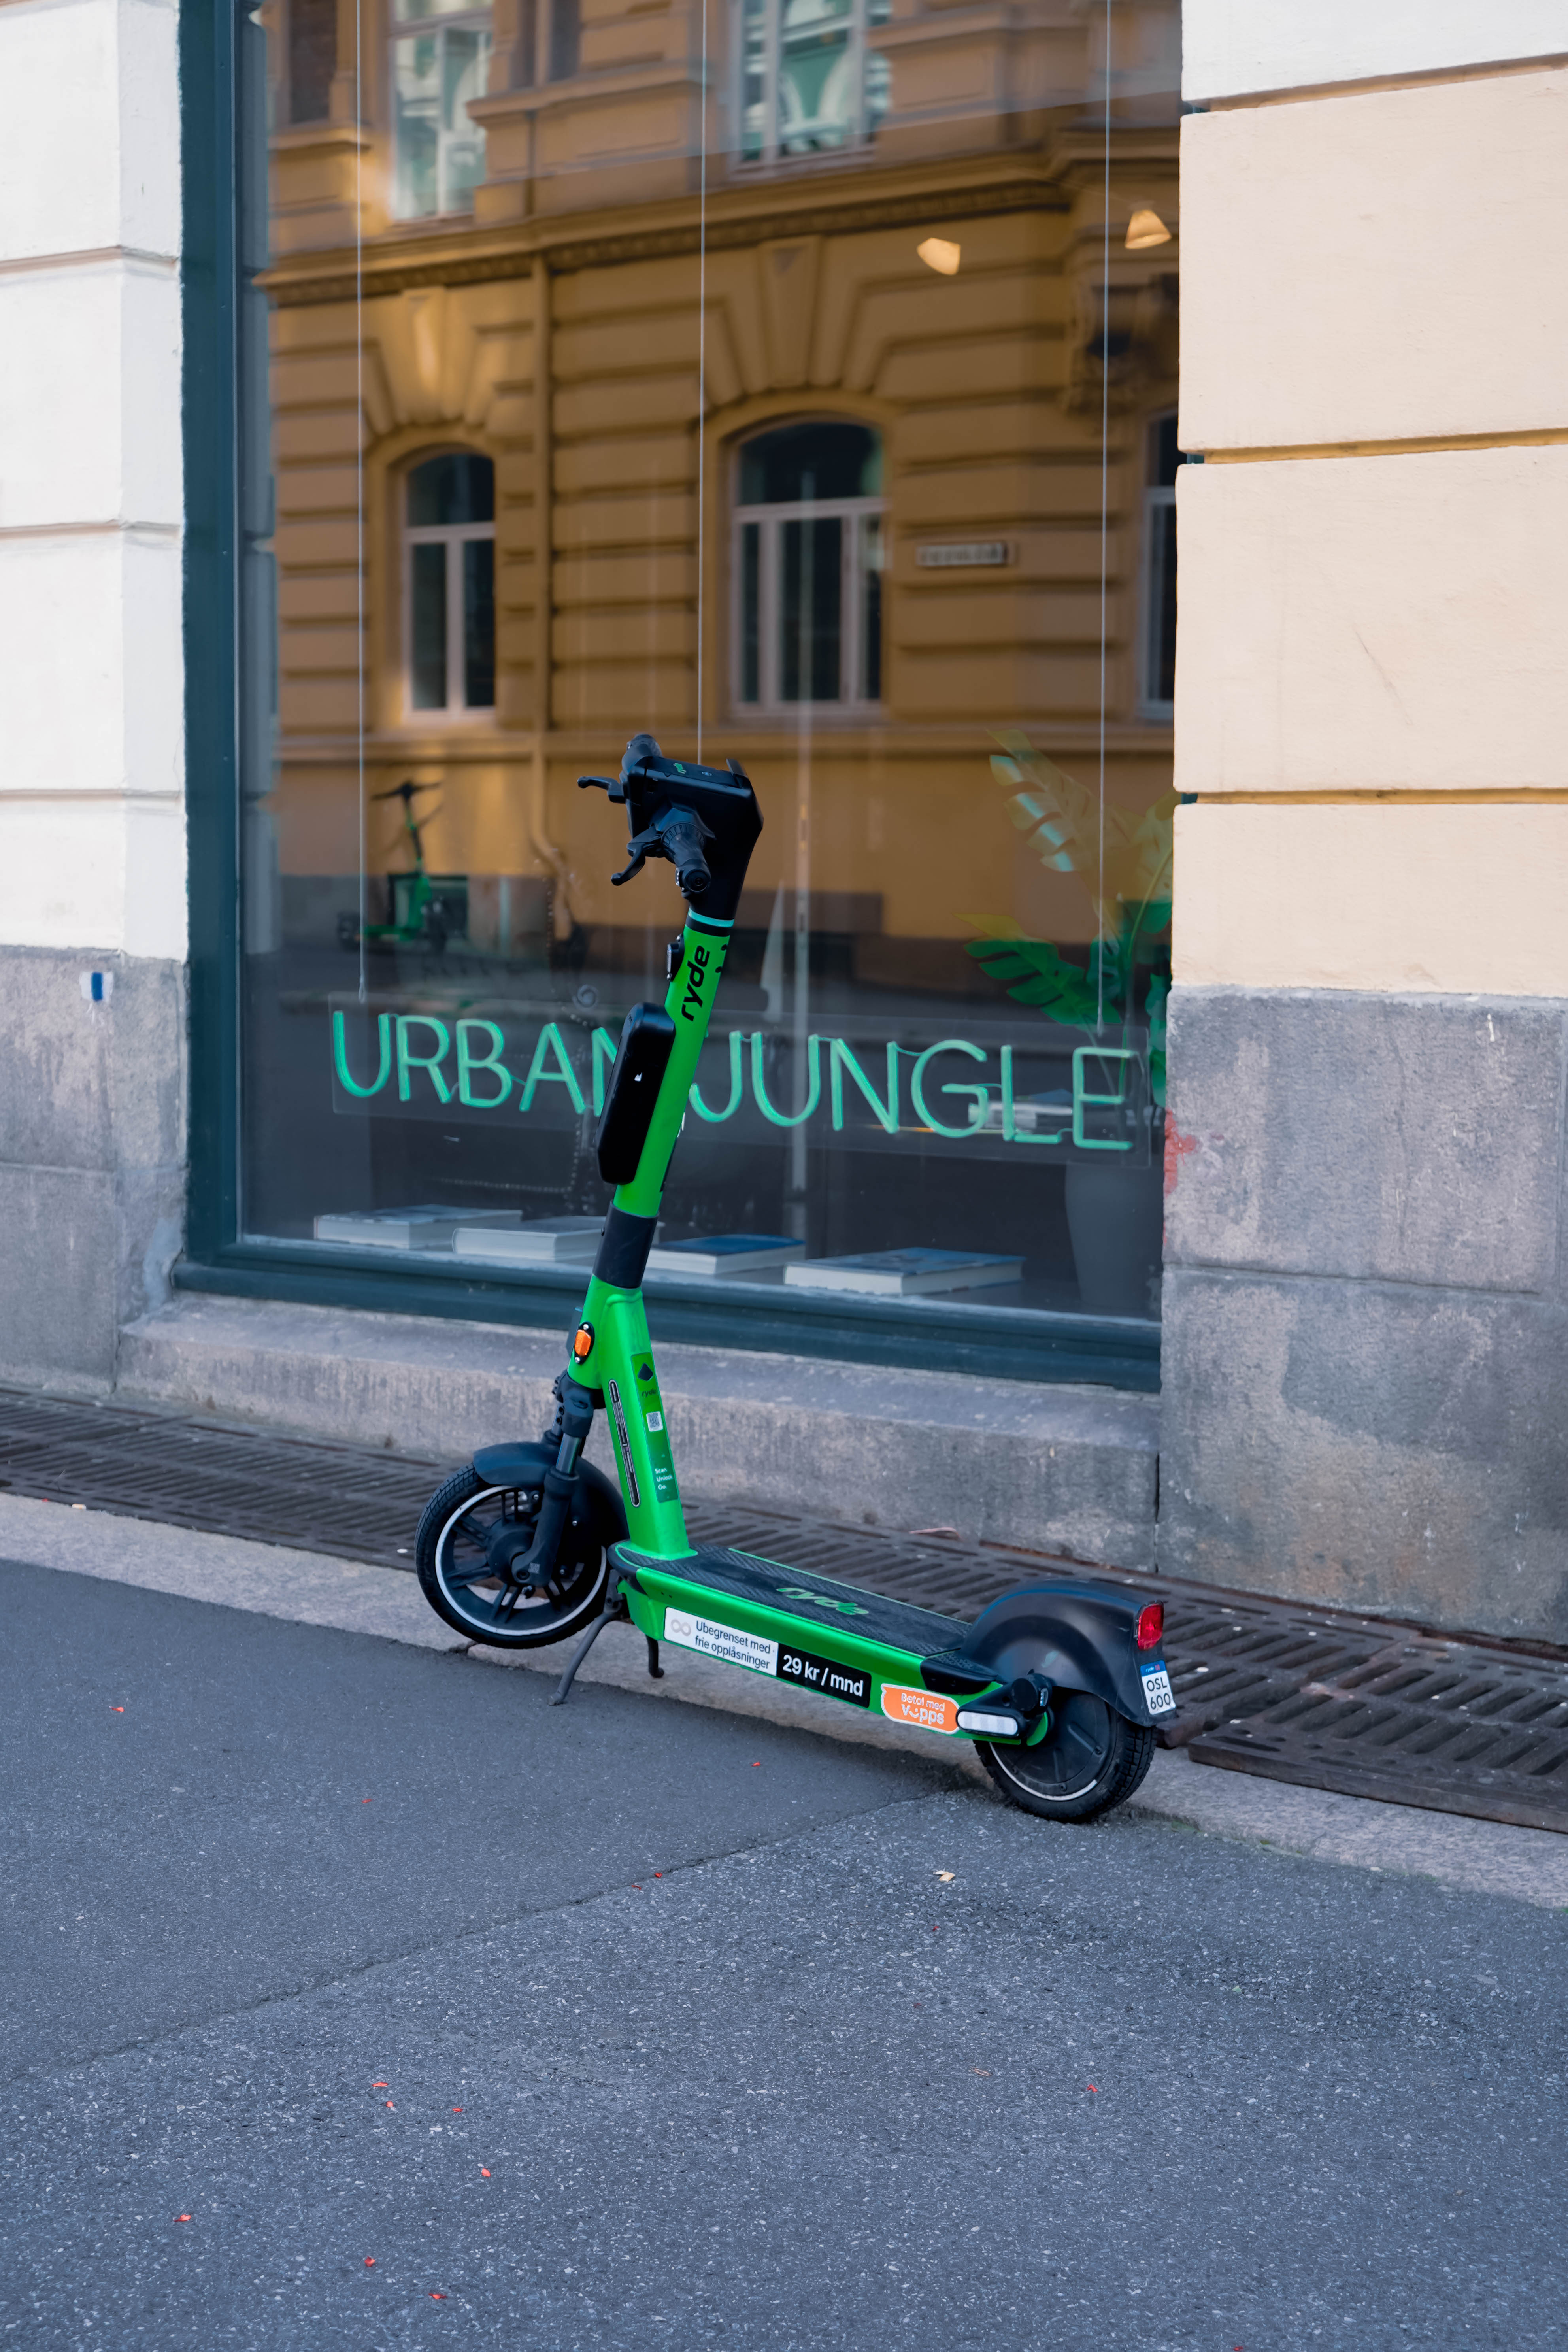
\includegraphics[width=\paperwidth,height=\paperheight]{src/Figures/Arriere_plan/Arriere_plan_Chap_4.jpg}
    }

% Rectangle
\AddToShipoutPictureBG*{
  \begin{tikzpicture}[remember picture,overlay]
    \node[fill=white, opacity=0.75, text width=\paperwidth, minimum height=11cm, anchor=north] 
    at ([yshift=-2cm]current page.north) {};
  \end{tikzpicture}
}

% Source
\AddToShipoutPictureFG*{
  \AtPageLowerRight{
    \raisebox{1cm}{
      \hspace{16cm}
      
\begin{tikzpicture}
        \node[fill=white, rounded corners=5pt, inner sep=5pt, align=center] {
          \tiny{Photographie~: \textcolor{blue}{Dylan Moinse (2023)}}
        };
      \end{tikzpicture}
    }
  }
}

    % ___________________________________________
    % Mini-sommaire
    \cleardoublepage
    \setcounter{tocdepth}{2}
    % Redéfinir le titre de la table des matières locale
    \renewcommand{\localcontentsname}{Table des matières du chapitre~4}
\localtableofcontents

% Réinitialiser numérotation section
\setcounter{section}{0}

    % ___________________________________________
    % Graphical abstract
    \newpage
\section*{Points clés du chapitre~4
    \label{chap4:graphical-abstract}
    }
    \markright{Préambule du chapitre}{}

\begin{figure}[h!]\vspace*{4pt}
        \caption*{}
        \label{graphical-abstract-chap4}
        \centerline{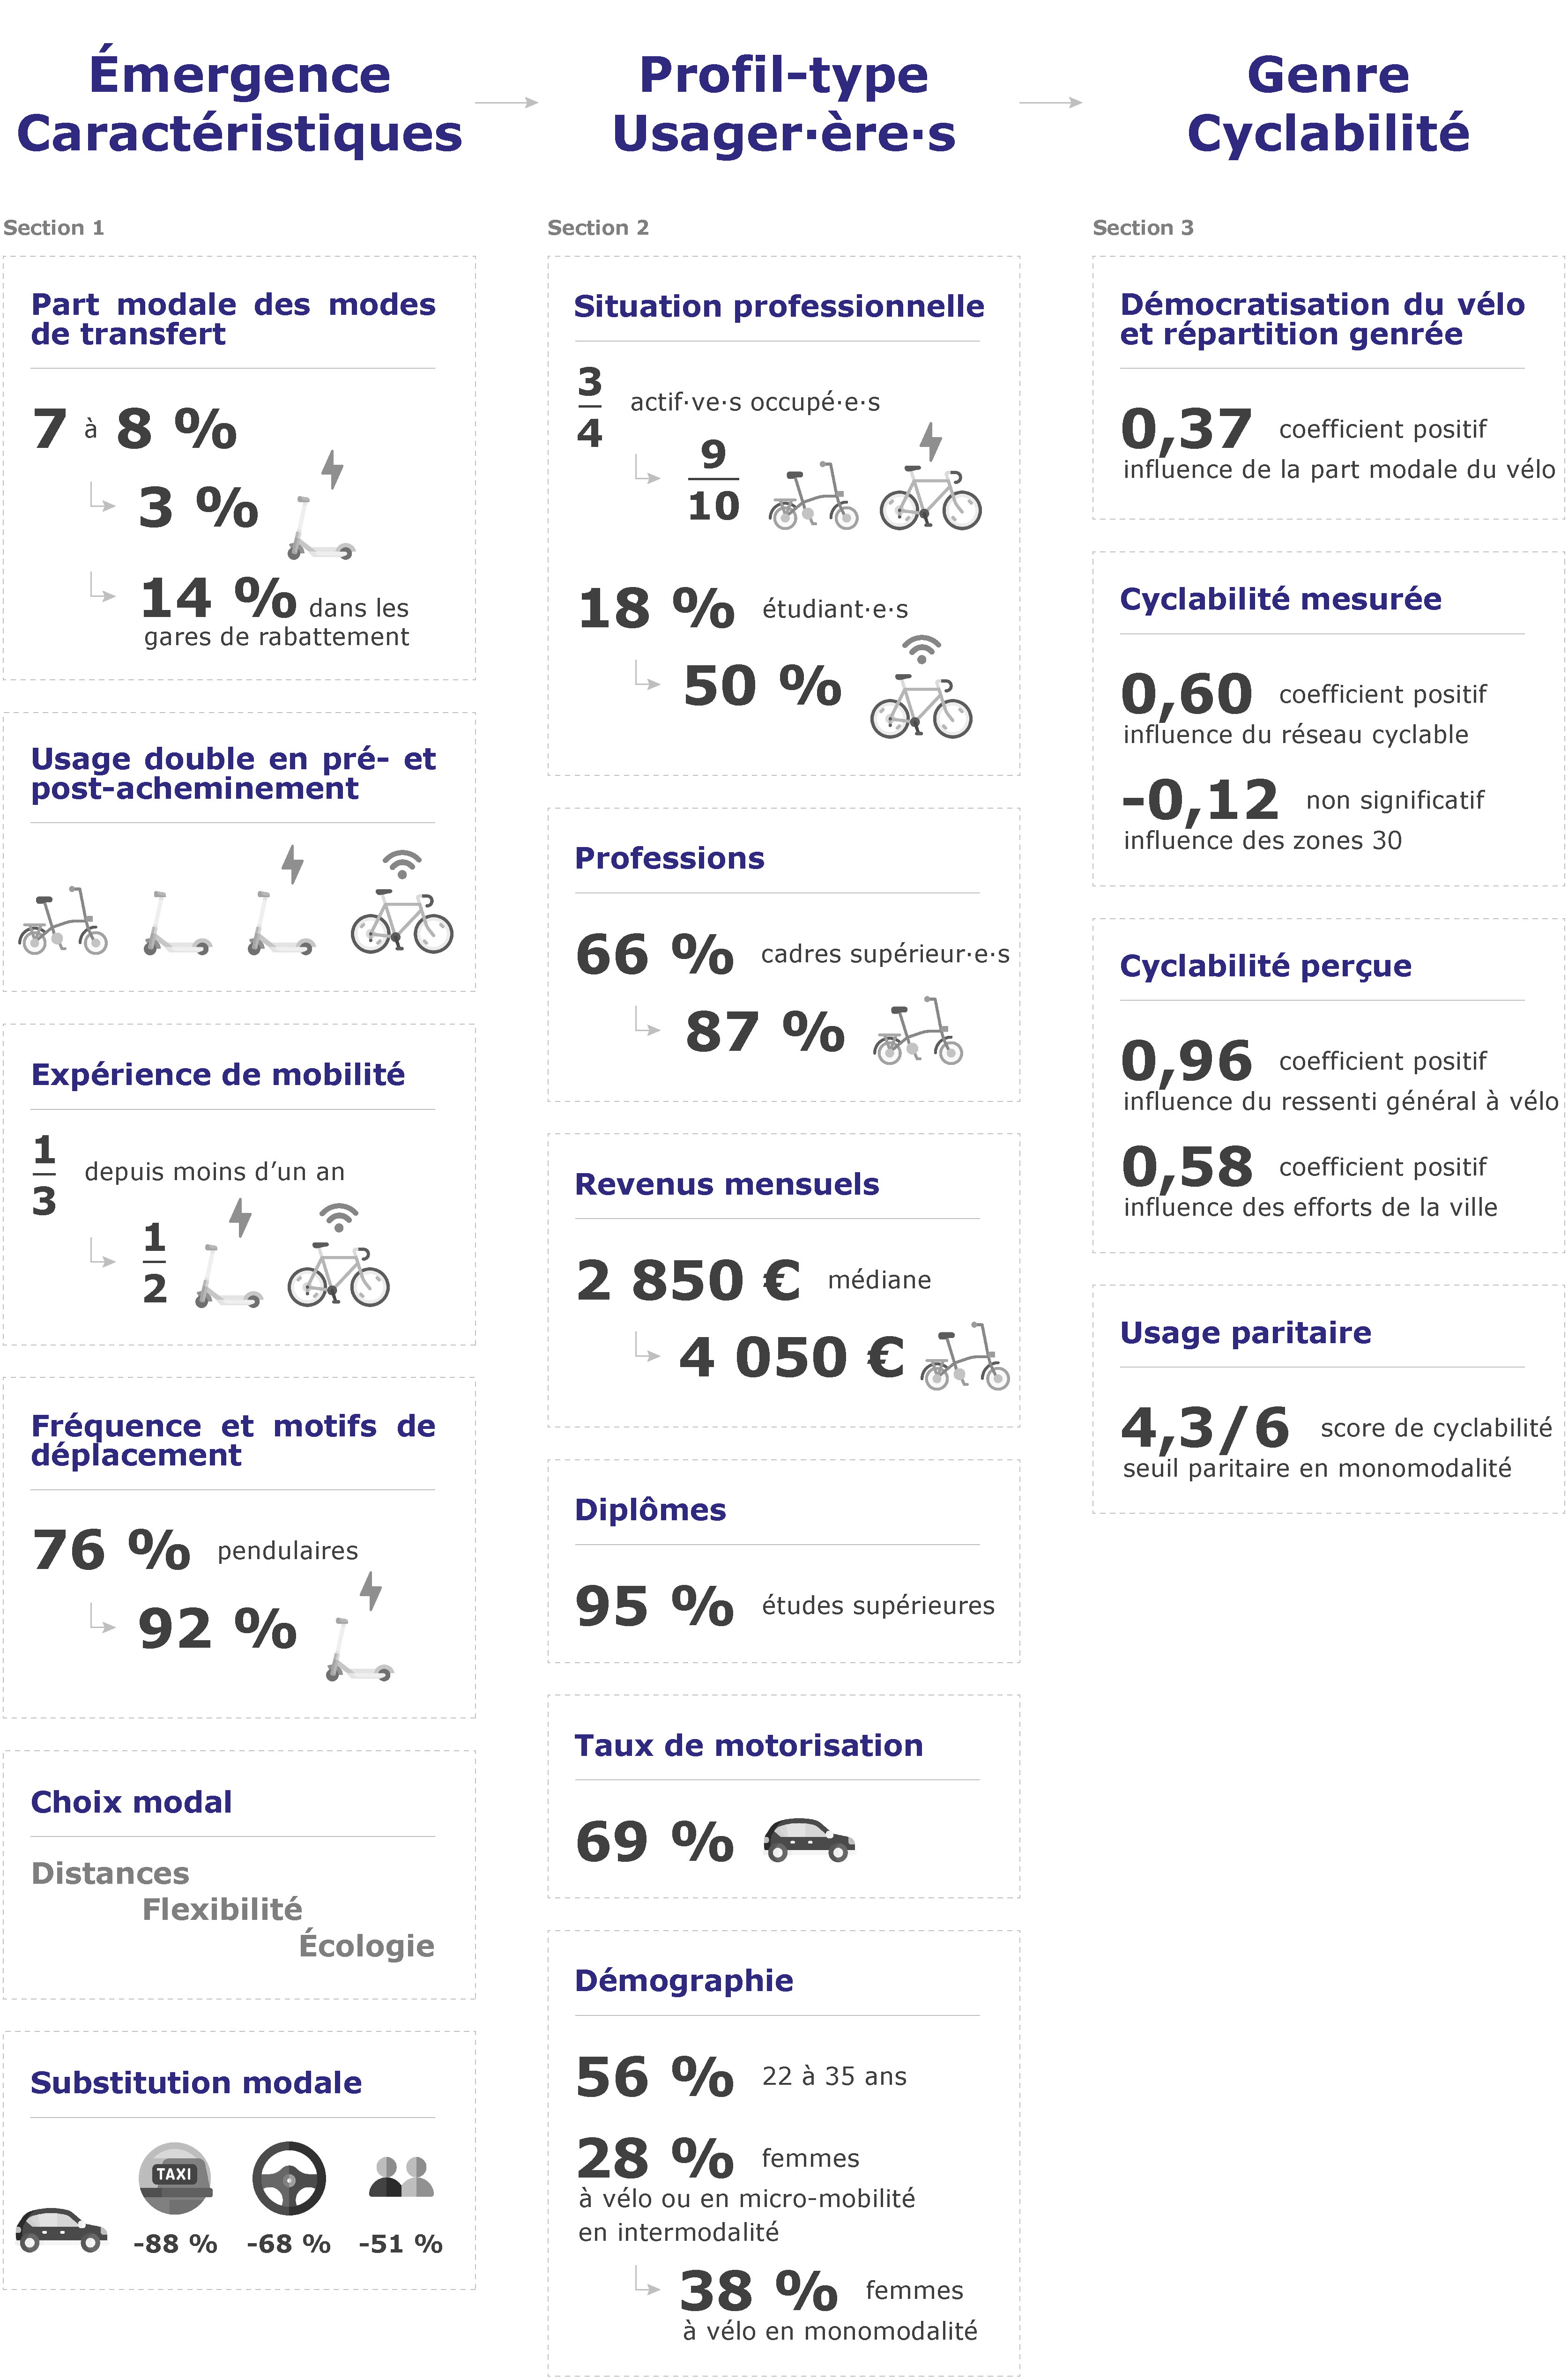
\includegraphics[width=1\columnwidth]{src/Figures/Graphical-abstract/FR_Graphical_abstract_chap4.pdf}}
        \vspace{5pt}
    \end{figure}

    % ___________________________________________
    % Préambule
    \newpage
    \begin{tcolorbox}[colback=white!5!white,
                      colframe=blue!75!blue,
                      title=
                      \bigskip
                      \center{\textbf{Préambule du chapitre~4}}
                      \\
                      \raggedright{\small{Chapitre composé de \pagedifference{chap4:titre}{chap5:titre} pages, dont \pagedifference{chap4:bibliographie}{chap5:titre} pages de bibliographie}}
                      \bigskip]
\Large{\textcolor{blue}{\textbf{Résumé~:}}}
    \\
    \small{
Ce chapitre explore l'émergence et la diversification de l'intégration de la mobilité individuelle légère dans les systèmes de transport en commun. L'accent est mis sur leur synergie modale en examinant les pratiques intermodales des usager·ère·s.%%Rédigé%%
    \\
La \hyperref[section-chap4:progression-velo-micromobilite-aubaine]{première section} (page~\pageref{section-chap4:progression-velo-micromobilite-aubaine}) vise à quantifier la part modale du vélo et de la micro-mobilité en association avec le système ferroviaire, en analysant les taux d'adoption en fonction des contextes géographiques et des segments de transfert, avant ou après le trajet principal. Les résultats montrent non seulement une part modale sous-estimée de ces modes de transfert avec le rail, estimée à 8~\%, mais également une tendance à la croissance de cet usage. Contrairement aux idées reçues, cette part modale est plus élevée dans les territoires périurbains que dans les centres urbains. L'adoption de ces pratiques intermodales est récente pour une proportion importante d'usager·ère·s et tend à remplacer l'utilisation du bus de transfert et de l'automobile, sans pour autant substituer la marche.%%Rédigé%%
    \\
Cependant, ces pratiques de mobilité demeurent inégalitaires, attirant principalement des hommes adultes, hautement qualifiés et à revenus relativement élevés. La \hyperref[section-chap4:profil-sociodemographique]{deuxième section} (page~\pageref{section-chap4:profil-sociodemographique}) repose ainsi sur la problématique de l'inclusivité des pratiques intermodales, en fournissant un profil socio-démographique des cyclistes intermodaux·les et en identifiant les potentiels de report modal vers ces solutions de mobilité.%%Rédigé%%
    \\
Enfin, la \hyperref[section-chap4:cyclabilite-genre]{troisième section} (page~\pageref{section-chap4:cyclabilite-genre}) présente une étude de cas sur les disparités de genre dans l'utilisation monomodale et intermodale de ces véhicules, en mettant en avant l'importance de la conception territoriale, de l'environnement urbain et de leur perception pour favoriser un accès plus équitable à ces modes de déplacement. La modélisation statistique identifie une association positive entre la cyclabilité perçue, la cyclabilité objective, la part modale du vélo et la proportion de femmes cyclistes, suggérant que l'amélioration du \Guillemets{système vélo} et du \Guillemets{perception générale} en matière de \Guillemets{climat vélo} est cruciale afin de promouvoir une utilisation plus inclusive du vélo et de la micro-mobilité.%%Rédigé%%
    }
    \tcblower
\Large{\textcolor{blue}{\textbf{Mots-clés~:}}}
    \\
    \small{
Choix modal~;
Comportements de mobilité~;
Compétitivité modale~;
Cyclabilité perçue~;
Déplacements pendulaires~;
Genre~;
Inégalités socio-économiques~;
Mobilité inclusive~;
Part modale~;
Pratiques émergentes
    }
    \end{tcolorbox}

    % ___________________________________________
    % 4.*.
    \newpage
    \needspace{1\baselineskip} % Réserve de l'espace
    \addcontentsline{toc}{section}{Introduction du chapitre~4}
    \sectionheader{Introduction du chapitre}
\section*{Introduction du chapitre~4
    \label{chap4:introduction}
    }
    \markright{Introduction du chapitre~4}{}

    % Citation
    \begin{displayquote}
\Guillemets{\textsl{Le paradigme de l'accessibilité dans la planification des transports et de l'aménagement du territoire s'est étroitement associé à la multimodalité et à une vision d'équité vis-à-vis de la mobilité.} [\dots] \textsl{L'accessibilité, en tant que ressource, représente le bénéfice recherché et offert par les systèmes de transport~; cette ressource peut être répartie de manière équitable ou non. Bien que toutes les populations profitent d'une amélioration de leur accessibilité, certaines partent d'une situation de déficit plus prononcé. Dans le cadre de cette réorientation vers l'accessibilité, l'analyse de la mobilité se focalise désormais sur la performance du système en fonction des besoins de la population plutôt qu'en se limitant aux infrastructure.}}\footnote{
    \Guillemets{\textsl{The accessibility paradigm in transportation and land-use planning has become closely associated with both multimodalism and an equity-based view of transportation.} [\dots] \textsl{Accessibility is a resource that is the desired benefit provided by transportation; that resource can be distributed equitably or inequitably. All populations benefit when their accessibility increases, though some populations start from a position of greater accessibility deficit. Under the accessibility shift, transportation analysis focuses on system performance with respect to population rather than with respect to pieces of infrastructure.}} \textcolor{blue}{\autocite[16-17]{levine_mobility_2019}}\index{Levine, Jonathan|pagebf}\index{Grengs, Joe|pagebf}\index{Merlin, Louis~A.|pagebf}.} [traduction libre]

\textcolor{blue}{Jonathan} \textcolor{blue}{\textcite[16-17]{levine_mobility_2019}}\index{Levine, Jonathan|pagebf}\index{Grengs, Joe|pagebf}\index{Merlin, Louis~A.|pagebf}. \foreignlanguage{english}{\textsl{From Mobility to Accessibility: Transforming Urban Transportation and Land-Use Planning}}, Cornell University Press, Ithaca, 240~p. ISBN~: \href{https://search.worldcat.org/fr/title/1393973234}{978-1-5017-1608-9}
    \end{displayquote}

    % Introduction
\lettrine[lines=3, findent=8pt, nindent=0pt]{\lettrinefont L}{e} premier chapitre, consacré aux résultats empiriques issus de cette recherche doctorale, engage une investigation des \textsl{pratiques intermodales} en tant qu'objets d'étude, caractérisées par l'intégration de la mobilité individuelle légère aux réseaux de \gls{transport en commun}. Cette rubrique scrute la dimension individuelle de l'\gls{accessibilité}, en explorant les évolutions actuelles des systèmes de mobilité ainsi que les comportements et le profil des usager·ère·s adoptant ces combinaisons modales. L'enjeu de cette étude est de démontrer la pertinence de ce sujet de recherche dans le contexte français, spécifiquement dans la région des Hauts-de-France, en pointant l'essor de ces modes de déplacement et de leurs interactions \textcolor{blue}{\autocites[77]{oostendorp_combining_2018}[56]{ensor_mode_2021}}\index{Oostendorp, Rebekka|pagebf}\index{Gebhardt, Laura|pagebf}\index{Ensor, Matt|pagebf}\index{Maxwell,~O.|pagebf}\index{Bruce, Oliver|pagebf} en pleine \Guillemets{hybridation modale} \textcolor{blue}{\autocite[15]{amar_homo_2016}}\index{Amar, Georges|pagebf}.%%Rédigé%%

    % Objectifs de recherche
Face à une méconnaissance générale de la \gls{micro-mobilité}, alors en pleine \Guillemets{émergence}, notamment en ce qui concerne la possession de véhicules personnels \textcolor{blue}{\autocites{richer_dossier_2021}[19]{pages_nouveaux_2021}}\index{Pages, Thibaud|pagebf}\index{Lammoglia, Adrien|pagebf}\index{Josselin, Didier|pagebf}\index{Richer, Cyprien|pagebf} et leurs connexions avec le transport public (voir les lacunes de la littérature identifiées dans le \hyperref[chap2:titre]{chapitre~2}, page~\pageref{chap2:titre}), ce chapitre vise à clarifier la place et la contribution de ces véhicules par rapport à la définition d'un \acrfull{M-TOD}, tout en offrant une vue d'ensemble des usager·ère·s. Ce travail de recherche repose ainsi sur les gares, lieux où sont observées des pratiques modales qui intègrent le \gls{vélo} et la micro-mobilité, dans le but de mettre en relief ce phénomène de mobilité, de plus en plus visible dans ces lieux d'échange stratégiques. La question centrale de cette recherche empirique est d'explorer et de caractériser les pratiques intermodales qui incluent la mobilité individuelle légère dans divers contextes territoriaux et à une échelle régionale, voire nationale. Trois objectifs viennent structurer le présent chapitre~:
\begin{customitemize}
    \item \textsl{Déterminer la part modale de la mobilité individuelle légère intégrée au système ferroviaire, en fonction des contextes géographiques}. Cette analyse quantifie l'adoption intermodale à partir d'estimations de la part modale du vélo et de la micro-mobilité en tant que modes de transfert, traitant leur émergence dans diverses configurations territoriales tout en distinguant les segments de pré-acheminement et de post-acheminement. L'originalité de cette approche réside dans sa capacité à comparer divers véhicules, une démarche peu fréquente dans la littérature~;
    \item \textsl{Étudier la dimension inclusive des pratiques intermodales}. Cette section établit un portrait des voyageur·se·s intermodaux·les, à partir d'une grille basée sur les capitaux, pour identifier le potentiel de report modal vers ces solutions de mobilité~;
    \item \textsl{Étude de cas sur la répartition genrée de l'usage exclusif et intermodal du vélo et de la micro-mobilité, en lien avec la conception territoriale}. Cette investigation se focalise sur la dimension inclusive de l'accessibilité connectée à la qualité d'aménagement des espaces publics, en définissant un modèle statistique qui capture les leviers pour réduire les inégalités d'accès à ces modes de déplacement. L'approche par l'\Guillemets{hospitalité territoriale} qui s'est enrichie et diversifiée au fil du temps sert de référentiel notionnel pour évaluer la conception territoriale ainsi que les politiques publiques, en matière d'accueil de cyclistes et de fidélisation des usager·ère·s en répondant à leurs besoins \textcolor{blue}{\autocite[3]{talandier_lhospitalite_2023}}\index{Talandier, Magali|pagebf}.
\end{customitemize}%%Rédigé%%

    % Annonce du plan 1
Nous commencerons par quantifier et caractériser les pratiques intermodales émergentes afin de comprendre en quoi elles constituent une opportunité pour les services de transport en commun (\hyperref[section-chap4:progression-velo-micromobilite-aubaine]{section~1}, page~\pageref{section-chap4:progression-velo-micromobilite-aubaine}). La première section évaluera la part modale de chacun des véhicules de la mobilité individuelle légère lorsqu'elle est intégrée au réseau ferroviaire, tout en contextualisant ces mesures en fonction du caractère urbain ou \gls{périurbain} du territoire et selon que le trajet à vélo ou en micro-mobilité s'inscrit dans une logique de \Guillemets{premier} ou de \Guillemets{dernier kilomètre} (\hyperref[chap4:proportion-croissante-voyageurs-intermodaux]{sous-section~1.1}, page~\pageref{chap4:proportion-croissante-voyageurs-intermodaux}). La seconde sous-section explorera les comportements de mobilité des cyclo-voyageur·se·s pour mieux saisir l'impact de l'adoption modale sur les systèmes de mobilité existants, en identifiant les motivations et les effets de substitution qui en découlent (\hyperref[chap4:comportements-mobilite]{sous-section~1.2}, page~\pageref{chap4:comportements-mobilite}).%%Rédigé%%

    % Annonce du plan 2
La seconde section dressera un portrait des cyclistes intermodaux·les, en les comparant aux voyageur·se·s ferroviaires dans leur ensemble et à la population française, afin d'identifier les spécificités de ce groupe social d'individus mobiles (\hyperref[section-chap4:profil-sociodemographique]{section~2}, page~\pageref{section-chap4:profil-sociodemographique}). Nous commencerons par examiner les ressources économiques, le statut professionnel et le niveau de qualification de ces usager·ère·s, en tenant compte des capitaux économiques et culturels à leur disposition (\hyperref[chap4:capital-economique-culturel]{sous-section~2.1}, page~\pageref{chap4:capital-economique-culturel}). Ensuite, nous dépeindrons les capitaux matériels et les pratiques de mobilité quotidienne, dans le but d'établir une photographie de ces individus (\hyperref[chap4:capital-mobilite]{sous-section~2.2}, page~\pageref{chap4:capital-mobilite}). Enfin, nous traiterons des attributs démographiques des cyclo-voyageur·se·s, en considérant les critères liés à l'âge et au \gls{genre}, dans une optique de mobilité inclusive (\hyperref[chap4:demographie]{sous-section~2.3}, page~\pageref{chap4:demographie}). Cette analyse préparera le terrain pour la dernière section de ce chapitre.

    % Annonce du plan 3
La troisième partie sondera les interactions entre l'usage genré de ces solutions de mobilité et le rôle modérateur de l'urbanisme, sous l'angle de l'hospitalité territoriale. Cette section explorera les dynamiques relationnelles entre les enjeux relatifs au genre et les aménagements urbains (\hyperref[section-chap4:cyclabilite-genre]{section~3}, page~\pageref{section-chap4:cyclabilite-genre}). Nous débuterons par la description du cadre d'analyse, élaboré à partir de l'exploitation de bases de données conjointement à celle de notre matériau empirique (\hyperref[chap4:materiau-empirique-genre]{section~3.1}, page~\pageref{chap4:materiau-empirique-genre}), qui prendra la forme d'une modélisation statistique (\hyperref[chap4:methodologie-modele-ols]{section~3.2}, page~\pageref{chap4:methodologie-modele-ols}). À partir de l'approche explicitée, nous présenterons les liens entre la cyclabilité, à la fois objective et perçue, et la pratique genrée de la mobilité individuelle légère (\hyperref[section-chap4:cyclabilite-territoires-genre]{section~3.3}, page~\pageref{section-chap4:cyclabilite-territoires-genre}).%%Rédigé%%

    % Annonce du plan 4
En guise de conclusion, nous restituerons les apports majeurs de cette étude veillant à esquisser un aperçu général des cyclistes et de leurs pratiques de mobilité, dans un contexte intermodal, ainsi qu'à recentrer les enjeux d'inclusivité sociale sous l'angle de l'aménagement des territoires (\hyperref[chap4:conclusion]{conclusion du chapitre~4}, page~\pageref{chap4:conclusion}).%%Rédigé%%


     % ___________________________________________
    % 4.1.
    \newpage
    \needspace{1\baselineskip} % Réserve de l'espace
    \sectionheader{Adoption croissante de la mobilité individuelle légère}
\section{La progression conjointe du vélo et de la micro-mobilité, une aubaine pour les réseaux de transport en commun
    \label{section-chap4:progression-velo-micromobilite-aubaine}
    }

    % Introduction
Les pratiques intermodales, consistant en la synergie modale du transport public et du vélo ainsi que de la micro-mobilité, sont appelées à se développer rapidement \textcolor{blue}{\autocite[4]{kostrzewska_towards_2017}}\index{Kostrzewska, Małgorzata|pagebf}\index{Macikowski, Bartosz|pagebf}, dans la mesure où elles satisfont les besoins de mobilité liés aux \Guillemets{premiers et derniers kilomètres} \textcolor{blue}{\autocite[29]{holm_moller_micromobility_2020}}\index{Holm Møller, Thomas|pagebf}\index{Simlett, John|pagebf}\index{Mugnier, Eric|pagebf}. Sur la base de cette projection, notre recherche vise à confirmer la première hypothèse selon laquelle le vélo connaît une renaissance et un redéploiement concomitant à l'expansion de la micro-mobilité, et à vérifier la seconde hypothèse qui postule que le renouveau du rapport aux proximités offre une opportunité pour les systèmes de transport en commun. En exploitant les données issues de l'observation quantitative et du questionnaire distribué aux usager·ère·s en gare, nous cherchons à dresser un portrait exhaustif de ces comportements de mobilité et à en interroger les implications. Cette démarche vise non seulement à fournir un aperçu détaillé des pratiques intermodales, mais aussi à poser les bases de discussions ultérieures sur leur intégration aux principes du \acrfull{TOD}.%%Rédigé%%

    % Annonce du plan
Cette première section dédiée à l'évolution de l'intégration de la mobilité individuelle légère, perçue comme une aubaine pour les réseaux de transport en commun, se déploie en deux phases distinctes. Dans un premier temps, nous examinerons la pertinence du terme \textsl{émergence} pour qualifier les pratiques intermodales observées (voir la \hyperref[chap4:proportion-croissante-voyageurs-intermodaux]{section consacrée à la proportion croissante de voyageur·se·s intermodaux·les}, page~\pageref{chap4:proportion-croissante-voyageurs-intermodaux}). Cette exploration comprendra une évaluation des parts modales attribuées à ces modes de transfert, en les croisant avec l'expérience intermodale des utilisateur·rice·s, la \gls{cartographie} des flux d'origine et de destination, ainsi que les spécificités de chaque segment des déplacements intermodaux. Par la suite, notre attention se portera sur les comportements de mobilité des cyclo-voyageur·se·s (voir la \hyperref[chap4:comportements-mobilite]{section sur les caractéristiques des navettes}, page~\pageref{chap4:comportements-mobilite}), dans le but de mieux saisir les contours de ces pratiques intermodales et d'en évaluer l'impact sur les systèmes de mobilité coexistants. Cela impliquera une analyse de la fréquence d'usage, en relation avec les motifs de \gls{déplacement}, les motivations derrière l'adoption de ces modes, l'effet de substitution modale et les changements de mobilité qui en découlent.%%Rédigé%%

    % 4.1.1.
    \needspace{1\baselineskip} % Réserve de l'espace
\subsection{Une proportion croissante de cyclo-voyageur·se·s, impulsée par la montée en puissance de la micro-mobilité à usage personnel et partagé
    \label{chap4:proportion-croissante-voyageurs-intermodaux}
    }

    % Introduction
Dans cette sous-section, nous sondons la dimension intermodale de la mobilité individuelle légère au sein du réseau ferroviaire régional, en mettant un accent particulier sur la manière dont des modes de déplacement émergents, tels que la \acrfull{TEP}, contribuent à renforcer l'attractivité et à améliorer l'accessibilité des systèmes de transport en commun \textcolor{blue}{\autocite[45]{corporate_partnership_board_good_2020}}\index{Corporate Partnership Board@\textsl{Corporate Partnership Board}|pagebf}, et ce, aussi bien dans les centres urbains que dans les territoires périurbains \textcolor{blue}{\autocite[38]{stransky_periurbain_2019}}\index{Stransky, Vaclav|pagebf}. Cette analyse est centrée sur les gares des Hauts-de-France où nous nous attachons à quantifier la part modale du vélo et de la micro-mobilité, en connexion avec les nœuds, de manière à illustrer leur importance croissante comme objets d'étude. Notre objectif est également de resituer les parts modales estimées de ces modes de transfert dans divers contextes urbains.%%Rédigé%%

    % 4.1.1.1.
    \needspace{1\baselineskip} % Réserve de l'espace
\subsubsection*{Part modale de la mobilité individuelle légère en association avec le réseau ferroviaire
    \label{chap4:part-modale-velo-micromobilite}
    }

    % Introduction
Au cours de cette recherche doctorale, une investigation sur neuf gares situées dans la région Hauts-de-France a d'abord permis de mettre en œuvre une observation quantitative, comme exposé dans la \hyperref[chap3:observation-quantitative-gares-examinees]{section méthodologique dédiée aux gares examinées} (page~\pageref{chap3:observation-quantitative-gares-examinees}) dans le \hyperref[chap3:titre]{chapitre~3} (page~\pageref{chap3:titre}). Cette analyse statistique a abouti à la constitution d'un échantillon descriptif comprenant 15~435 voyageur·se·s ferroviaires. Parmi ces usager·ère·s, 1~035 individus, représentant 6,71~\% de l'échantillon total, ont été identifiés accompagnés d'un vélo ou d'une option de micro-mobilité sur les quais.%%Rédigé%%

    % Part modale globale de l'embarquement (observation)
Cette observation suggère que, durant les périodes d'affluence généralement associées aux déplacements professionnels et scolaires ainsi que dans les gares sélectionnées considérées représentatives de la diversité des contextes urbains de la région, moins de 7~\% des passager·ère·s du \acrfull{TGV}, du \acrfull{TERGV} et du \acrfull{TER} emportent un moyen de transport relevant de la mobilité individuelle légère\footnote{
    Notons que cette proportion exclut les cyclo-voyageur·se·s ayant stationné leur véhicule avant de monter dans le train ou qui le récupèrent à leur descente du train, ainsi que les services de mobilité partagée.
}.%%Rédigé%%

    % Part modale détails de l'embarquement (observation)
Dans le cadre de cette étude sur les modalités d'embarquement des modes de déplacement légers à bord des trains, les séances d'observation indiquent une prédominance de la trottinette de tous types, représentant 3,65~\% (564 observations) du total. Elle est suivie de près par le vélo, toutes catégories confondues, qui comptabilise 2,93~\% (452 observations) des cas observés. Les autres formes de dispositif d'\acrfull{EDP} constituent 0,12~\% (19 observations). Plus spécifiquement, la répartition des types de mobilité individuelle légère embarquée se présente comme suit (voir l'\hyperref[fig-chap4:part-modale-detaillee-mobilite-individuelle-legere]{illustration \ref{fig-chap4:part-modale-detaillee-mobilite-individuelle-legere}}, page~\pageref{fig-chap4:part-modale-detaillee-mobilite-individuelle-legere}). La \acrshort{TEP} figure en tête avec 2,98~\% (460 observations), démontrant son adoption rapide et massive, surpassant même le vélo classique dans le contexte ferroviaire. Ce dernier détient une part modale qui s'établit à 2,13~\% (329 observations) en transfert. Le vélo pliant et la trottinette mécanique comptent respectivement 0,80~\% et 0,67~\% (122 et 104 observations), tandis que le \textsl{skateboard} et le monoroue sont nettement moins représentés, avec respectivement 0,07~\% et 0,05~\% (11 et 8 observations). Ces résultats statistiques soulignent que la \acrshort{TEP} s'avère être un mode de déplacement reconnu pour être particulièrement adapté pour l'embarquement à bord des trains, compte tenu de sa légèreté et de sa compacité.%%Rédigé%%

    % Figure part modale détaillée
    \begin{figure}[h!]\vspace*{4pt}
        \caption{Estimation de la part modale de la mobilité individuelle légère embarquée et intégrée au train, dans la région Hauts-de-France.}
        \label{fig-chap4:part-modale-detaillee-mobilite-individuelle-legere}
        \centerline{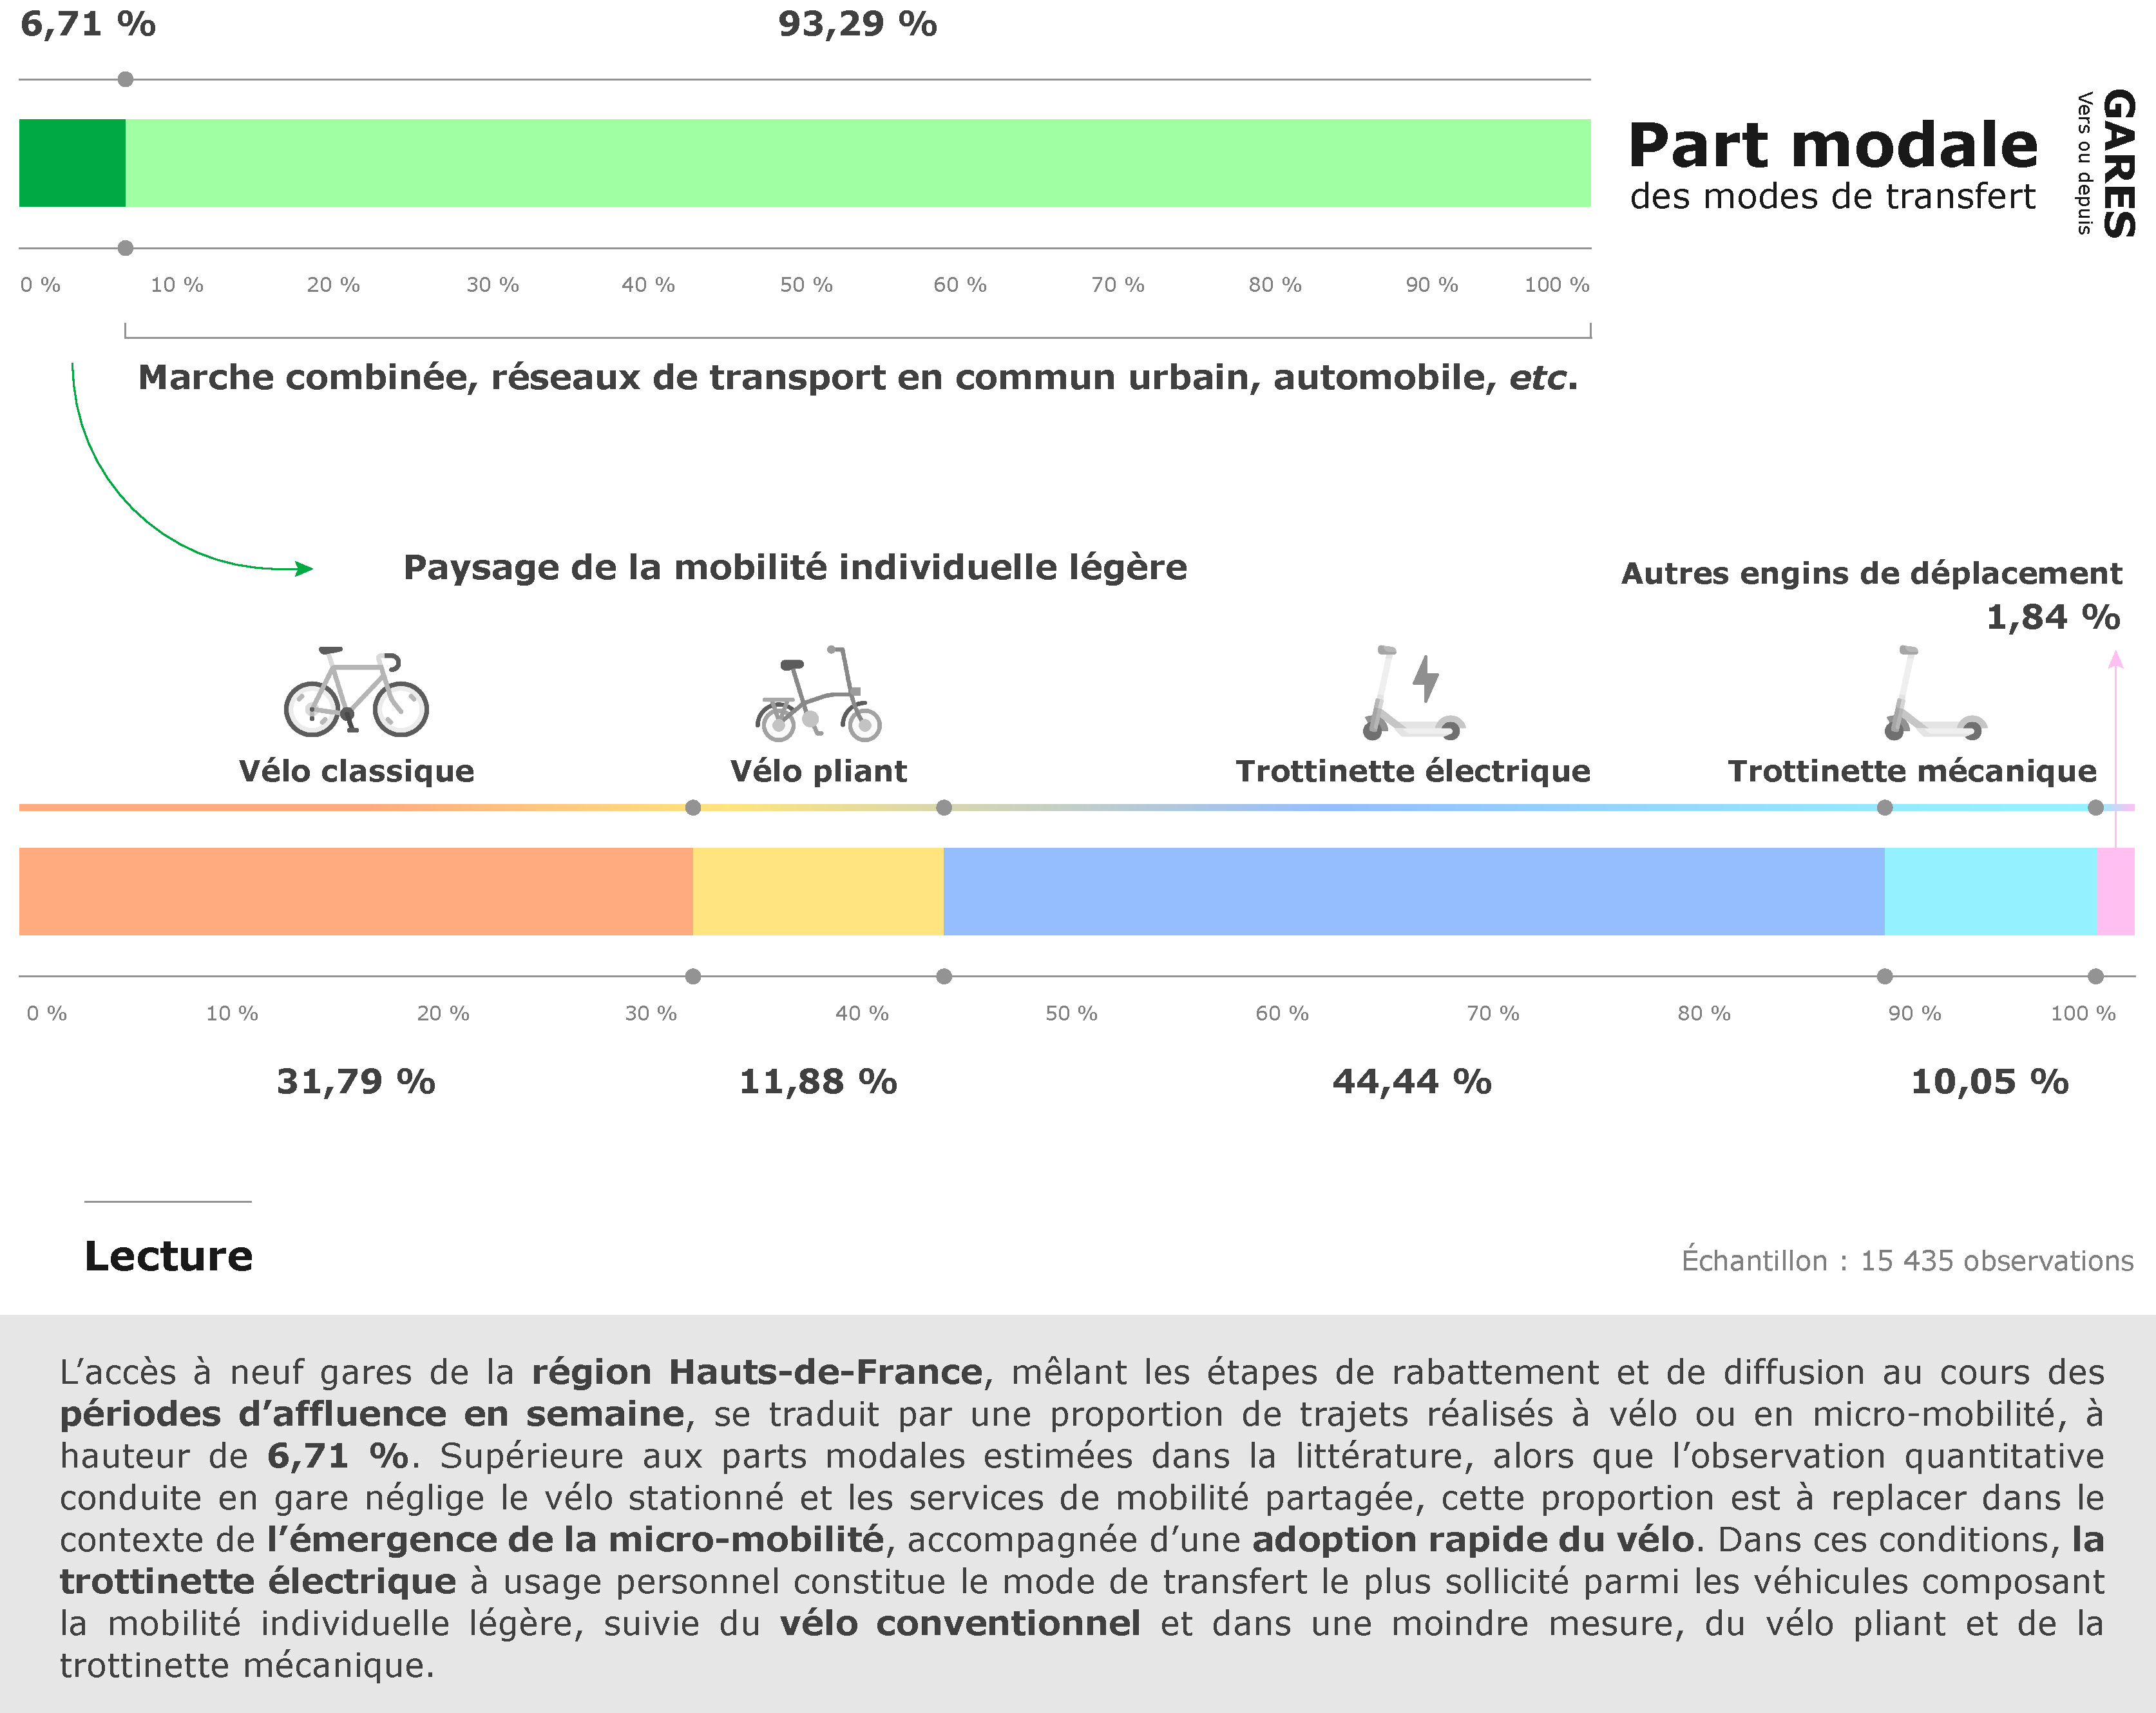
\includegraphics[width=1\columnwidth]{src/Figures/Chap-4/FR_Observation_quantitative_part_modale.pdf}}
        \vspace{5pt}
        \begin{flushright}\scriptsize{
        Auteur~: \textcolor{blue}{Dylan Moinse (2022)}
        }\end{flushright}
    \end{figure}

    % Part modale globale intermodale (questionnaire)
La quantification de l'usage intermodal de la mobilité individuelle légère a été enrichie par les données recueillies à l'aide du questionnaire adressé aux usager·ère·s\footnote{
    Il convient néanmoins de nuancer l'apport du questionnaire, en perspective de l'observation directe, en tenant compte du plus faible échantillon récolté et de l'échelle nationale incluant une diversité plus importante de systèmes de transport en commun, même si le \acrshort{TGV} et le \acrshort{TER} restent prédominants.
}. Comme représenté sur le \hyperref[table-chap4:part-modale-vehicules-intermodalite]{tableau~\ref{table-chap4:part-modale-vehicules-intermodalite}} (page~\pageref{table-chap4:part-modale-vehicules-intermodalite}), sur 100 voyageur·se·s ferroviaires impliqué·e·s dans un parcours intermodal intégrant la mobilité individuelle légère, 68 d'entre elleux ont déclaré utiliser un vélo (147 réponses), tandis que 22 ont opté pour une trottinette (48 réponses), 7 pour un service de vélo ou de micro-mobilité (16 réponses) et 3 pour une autre forme d'\acrshort{EDP} (6 réponses). Parmi ces voyageur·se·s intermodaux·les, 78~\% ont embarqué leur véhicule sur le réseau ferré (169 réponses). 50~\% des usager·ère·s ont opté pour un vélo conventionnel (110 réponses), avec un quart de ces cyclistes ayant choisi de stationner leur vélo. En ce qui concerne l'utilisation de la \acrshort{TEP}, celle-ci a été adoptée par 18~\% des répondant·e·s (39 réponses). 11~\% d'entre elleux se sont déplacé·e·s avec un vélo pliant mécanique (24 réponses). Notons que l'intégralité des répondant·e·s ayant eu recours à ces deux véhicules pliants les ont systématiquement embarqués à bord des services de \textsl{mass transit}.%%Rédigé%%

    % Tableau Part modale intermodale - modes de transfert
% Tableau Part modale intermodale - modes de transfert
%%Rédigé%%
    \begin{table}[h!]
    \centering
    \renewcommand{\arraystretch}{1.5}
    \resizebox{\columnwidth}{!}{
    \begin{tabular}{p{0.50\columnwidth}p{0.15\columnwidth}p{0.17\columnwidth}p{0.18\columnwidth}}
        %\hline
    \rule{0pt}{15pt} \small{\textbf{\textcolor{blue}{Type de véhicule}}} & \small{\textbf{\textcolor{blue}{Observation}}} & \small{\textbf{\textcolor{blue}{Questionnaire}}} & \small{\textbf{\textcolor{blue}{Embarquement}}}\\
        \hline
\small{\textbf{Tous types de mobilité individuelle légère confondus}} & \multirow{1.5}{*}{\small{\textbf{100,00~\%}}} & \multirow{1.5}{*}{\small{\textbf{100,00~\%}}} & \multirow{1.5}{*}{\small{\textbf{77,88~\%}}}\\
        \hdashline
\small{\textbf{Tous types de vélo personnel}} & \small{\textbf{43,67~\%}} & \small{\textbf{67,74~\%}} & \small{\textbf{78,91~\%}}\\
\small{Vélo conventionnel} & \small{31,79~\%} & \small{49,77~\%} & \small{75,93~\%}\\
\small{Vélo pliant} & \small{11,88~\%} & \small{11,06~\%} & \small{100,00~\%}\\
\small{Vélo à assistance électrique (\acrshort{VAE})} & \small{-} & \small{3,69~\%} & \small{50,00~\%}\\
\small{Vélo pliant électrique} & \small{-} & \small{2,76~\%} & \small{100,00~\%}\\
\small{Vélo cargo} & \small{-} & \small{0,46~\%} & \small{0,00~\%}\\
        \hdashline
\small{\textbf{Tous types de trottinette personnelle}} & \small{\textbf{54,49~\%}} & \small{\textbf{22,12~\%}} & \small{\textbf{100,00~\%}}\\
\small{Trottinette électrique personnelle (\acrshort{TEP})} & \small{44,44~\%} & \small{17,97~\%} & \small{100,00~\%}\\
\small{Trottinette mécanique} & \small{10,05~\%} & \small{4,15~\%} & \small{100,00~\%}\\
        \hdashline
\small{\textbf{Autres types d'\acrfull{EDP}}} & \multirow{1.5}{*}{\small{\textbf{1,84~\%}}} & \multirow{1.5}{*}{\small{\textbf{2,76~\%}}} & \multirow{1.5}{*}{\small{\textbf{83,33~\%}}}\\
\small{\textsl{Skateboard}} & \small{1,06~\%} & \small{1,38~\%} & \small{100,00~\%}\\
\small{Monoroue} & \small{0,77~\%} & \small{0,92~\%} & \small{100,00~\%}\\
\small{Gyropode} & \small{-} & \small{0,46~\%} & \small{0,00~\%}\\
        \hdashline
\small{\textbf{Tous types de véhicule partagé}} & \small{\textbf{-}} & \small{\textbf{7,37~\%}} & \small{\textbf{0,00~\%}}\\
\small{Vélo en libre-service (\acrshort{VLS})} & \small{-} & \small{6,45~\%} & \small{0,00~\%}\\
\small{Vélo électrique en \textsl{free-floating} (\acrshort{VFF})} & \small{-} & \small{0,46~\%} & \small{0,00~\%}\\
\small{Trottinette électrique en \textsl{free-floating} (\acrshort{TEFF})} & \multirow{1.5}{*}{\small{-}} & \multirow{1.5}{*}{\small{0,46~\%}} & \multirow{1.5}{*}{\small{0,00~\%}}\\
        \hline
        \end{tabular}}
    \caption{Part de chaque véhicule de transfert composant la mobilité individuelle légère, en France.}
    \label{table-chap4:part-modale-vehicules-intermodalite}
        \vspace{5pt}
        \begin{flushleft}\scriptsize{
        \textcolor{blue}{Note~:} la colonne \textsl{Observation} se réfère au sous-échantillon obtenu à partir de l'observation quantitative des voyageur·se·s (1~035 comptages), tandis que la colonne \textsl{Questionnaire} se rapporte aux déplacements intermodaux déclarés par les participant·e·s (217 réponses) et la modalité \textsl{Embarquement}, liée au questionnaire, quantifie la part de véhicules emportés à bord du transport public.
        \\
        \textcolor{blue}{Lecture~:} la répartition modale des cycles utilisés pour les transferts intermodaux montre que la trottinette électrique et le vélo, notamment pliant, à usage personnel, ont les parts les plus importantes. Le véhicule électrique et le vélo pliant, conventionnel comme électrique, ainsi que les dispositifs de mobilité légère tels que le \textsl{skateboard} et le monoroue, affichent un taux d'embarquement à 100~\%.
        }\end{flushleft}
        \begin{flushright}\scriptsize
        Auteur~: \textcolor{blue}{Dylan Moinse (2022)}
        \end{flushright}
        \end{table}%%Rédigé%%

    % Confrontation questionnaire
Les données extraites du questionnaire fournissent un éclairage complémentaire sur les écarts observés dans l'usage combiné de la mobilité individuelle légère avec le transport public. L'analyse met en relief la différence remarquée des parts modales du vélo, comparativement aux résultats de l'observation quantitative, qui peut s'expliquer par le non-recensement des vélos stationnés au cours des séances d'observation. Par ailleurs, l'écart considérable marquant la \acrshort{TEP} suggère que les réponses au questionnaire pourraient ne pas refléter fidèlement les pratiques intermodales telles qu'elles sont observées en gare. Cette distorsion pourrait découler d'une surreprésentation des cyclistes parmi les répondant·e·s, laissant supposer que les membres de cette communauté ont été particulièrement enclin·e·s à participer au questionnaire. Il apparaît clairement que le vélo, dans ses diverses formes et avec ses différentes modalités de stationnement ou d'embarquement, joue un rôle prépondérant dans l'usage intermodal de la mobilité individuelle légère. À cet effet, la \Guillemets{petite reine} contribue à hauteur de 45~\% à 70~\% de ces pratiques intermodales. D'autre part, la \acrshort{TEP} représente entre 20~\% et 45~\% des comportements observés et déclarés.%%Rédigé%%

    % Part modale déterminée
En intégrant les renseignements issus du questionnaire et en extrapolant les parts modales observées, nous sommes en mesure d'établir une estimation globale de la part modale de la mobilité individuelle légère, en tant que modes de transfert vers et depuis les gares de la région Hauts-de-France. Selon les réponses au questionnaire, environ un quart des navetteur·se·s optent pour le stationnement de leur véhicule léger, notamment du côté des cyclistes. En conséquence, la part modale du vélo en \gls{intermodalité} serait réévaluée à 2,64~\% (408 usager·ère·s) parmi l'ensemble des flux de voyageur·se·s. À cela, nous avons ajouté un sous-groupe d'utilisateur·rice·s des systèmes de \acrfull{VLS}, \acrfull{VFF} et de \acrfull{TEFF}, à hauteur de 7,37~\% (89 usager·ère·s). Ce qui porte le total à 1~202 cyclo-voyageur·se·s, nous permettant de conclure que la part modale estimée atteint 7,79~\%. Cette analyse fournit ainsi une vue plus complète et ajustée de l'utilisation de la mobilité individuelle légère dans le contexte intermodal.%%Rédigé%%

    % Littérature part modale vélo
La littérature scientifique et technique relative à la détermination de la fréquentation des gares par les cyclistes en rabattement est abondante et vient corroborer les résultats obtenus, qui nous ont permis de l'évaluer, pour le vélo classique, à 2,64~\% dans les gares étudiées en France. Concernant les gares des Hauts-de-France, une étude récente de \textcolor{blue}{\textcite[20]{hasiak_estimation_2023}}\index{Hasiak, Fabrice|pagebf}\index{Verdier, Laurent|pagebf} rapporte une part modale du vélo classique de 2~\% en \gls{rabattement} et de 1~\% en \gls{diffusion}, basée sur l'agrégation de diverses données d'enquête. Dans l'étude de cas spécifique de la gare d'Amboise (Centre-Val de Loire), 7~\% des voyageur·se·s accédant à la gare le font à vélo, la moitié emportant leurs véhicules tandis que l'autre moitié les stationnant \textcolor{blue}{\autocite[744]{midenet_modal_2018}}\index{Midenet, Sophie|pagebf}\index{Côme, Etienne|pagebf}\index{Papon, Francis|pagebf}. Au niveau national, la SNCF estime que 6~\% des client·e·s du \acrshort{TER} se déplacent à vélo pour rejoindre une gare \textcolor{blue}{\autocite[9]{coue_embarq_2021}}\index{Coué, Antoine|pagebf}. Cette proportion est à mettre en perspective avec celle observée aux Pays-Bas où 30~\% des accès aux nœuds régionaux se font à vélo, contre 25~\% au Danemark, 16~\% en Allemagne et 3~\% au Royaume-Uni \textcolor{blue}{\autocite[285]{martens_bicycle_2004}}\index{Martens, Karel|pagebf}. Par ailleurs, nous avons été en mesure d'identifier une proportion d'embarquement du vélo classique atteignant 76~\%, soit des comportements de mobilité bien plus marqués que ceux avancés par \textcolor{blue}{Christian} \textcolor{blue}{\textcite[5]{gioria_etude_2016}}\index{Gioria, Christian|pagebf}, qui révèlent que seulement 30~\% à 50~\% des déplacements intermodaux à vélo impliquent une phase d'emport sur certaines lignes \acrshort{TER}.%%Rédigé%%

    % Littérature part modale mobilité individuelle légère
Concernant l'intégration de la micro-mobilité, l'estimation de la répartition des modes de transfert est également consolidée par l'analyse secondaire de l'enquête par questionnaire, que nous avons réalisée dans la région Provence-Alpes-Côte d'Azur, qui met en évidence une part modale de 5~\% pour le vélo et de 2~\% pour la \acrshort{TEP} \textcolor{blue}{\autocite[180]{moinse_intermodal_2022}}\index{Moinse, Dylan|pagebf}\index{Goudeau, Matthieu|pagebf}\index{L'Hostis, Alain|pagebf}\index{Leysens, Thomas|pagebf}. De manière correspondante, 6~\% des flux vers et depuis les gares centrales en France sont réalisés à vélo ou en trottinette, qu'ils soient personnels ou en libre-service, d'après l'étude menée par le cabinet \textcolor{blue}{\textcite[18]{enov_enquete_2021}}\index{Enov@\textsl{Enov}|pagebf}. Par ailleurs, \textcolor{blue}{Christian} \textcolor{blue}{\textcite[5]{gioria_etude_2016}}\index{Gioria, Christian|pagebf} souligne que, bien que la fréquentation des gares à l'échelle nationale soit d'environ 2~\% pour la mobilité individuelle légère, ces chiffres varient significativement selon les régions, avec une part de 6~\% pour les gares en connexion directe avec un mode de transport lourd en milieu urbain.%%Rédigé%%

    % Transition
Les résultats statistiques de cette sous-section mettent en évidence une part modale relativement élevée de la mobilité individuelle légère, estimée à 8~\%, supérieure à celle généralement rapportée dans les études antérieures, à hauteur d'environ 2~\% à 3~\% en transfert. Ce constat peut alors s'expliquer par une meilleure prise en compte de la micro-mobilité, notamment de la \acrshort{TEP}, dans l'analyse des modes de transfert. La mise en lumière de ces pratiques fréquemment ignorées souligne l'intérêt de les intégrer dans les stratégies urbaines de type \acrshort{TOD}. Cependant, cette reconnaissance n'est pas suffisante pour attester de la nouveauté de ces pratiques intermodales, la simple identification de leur prévalence ne démontrant pas nécessairement une \textsl{émergence}. À cet égard, l'analyse qui suit repose sur les réponses au questionnaire distribué aux usager·ère·s intermodaux·les et vise à déterminer si l'adoption modale est récente ou au contraire bien établie, selon les différents modes de déplacement examinés.%%Rédigé%%

    % 4.1.1.2.
    \needspace{1\baselineskip} % Réserve de l'espace
\subsubsection*{Caractère émergent des pratiques intermodales en gare
    \label{chap4:emergence-pratiques-intermodales}
    }

    % Introduction
Face aux écarts observés entre la part modale de ces modes de transfert, déterminée par l'observation quantitative et les réponses au questionnaire, et les chiffres tirés des rares enquêtes traitant de ce sujet, il est légitime de s'interroger sur l'identification d'une tendance ces dernières années. Peut-on qualifier les pratiques de mobilité consistant à associer la mobilité individuelle légère avec les réseaux de transport en commun comme \textsl{émergentes}~? Pour aborder cette réflexion, nous avons examiné une question spécifique de l'enquête conduite, qui interroge les participant·e·s sur leur expérience intermodale~: \Guillemets{Depuis combien de temps avez-vous recours à cette combinaison modale~?} (voir l'\hyperref[annexes:structure-questionnaire-usagers]{annexe~\ref{annexes:structure-questionnaire-usagers}}, page~\pageref{annexes:structure-questionnaire-usagers}). L'objectif est alors de déterminer si les pratiques observées sont un phénomène récent, impulsé notamment par la diversification de la mobilité individuelle légère et par le développement de l'électromobilité.%%Rédigé%%

    % Résultats globaux expérience intermodale
Partant du constat d'une montée en puissance des pratiques intermodales en gare ces dernières années, attribuable principalement à l'irruption de la micro-mobilité, une attention particulière a été portée à l'expérience intermodale de ces voyageur·se·s (voir l'\hyperref[fig-chap4:experience-intermodale]{illustration~\ref{fig-chap4:experience-intermodale}}, page~\pageref{fig-chap4:experience-intermodale}). Les données descriptives tirées des réponses déclarées révèlent que pour 43~\% des participant·e·s, englobant tous les types de mobilité individuelle légère, ces combinaisons modales articulées avec les réseaux ferrés ont été adoptées depuis \Guillemets{plusieurs années} (94 réponses). En outre, respectivement 21~\% et 16~\% des individus interrogés ont une expérience intermodale datant respectivement d'environ \Guillemets{un an} et de \Guillemets{quelques mois} seulement (45 et 35 réponses). Par ailleurs, 13~\% des répondant·e·s se sont essayé.e.s pour la première fois à cette combinaison modale lors de l'administration du questionnaire (29 réponses).%%Rédigé%%

    % Figure expérience intermodale
    \begin{figure}[h!]\vspace*{4pt}
        \caption{Expérience intermodale déclarée des cyclo-voyageur·se·s.}
        \label{fig-chap4:experience-intermodale}
        \centerline{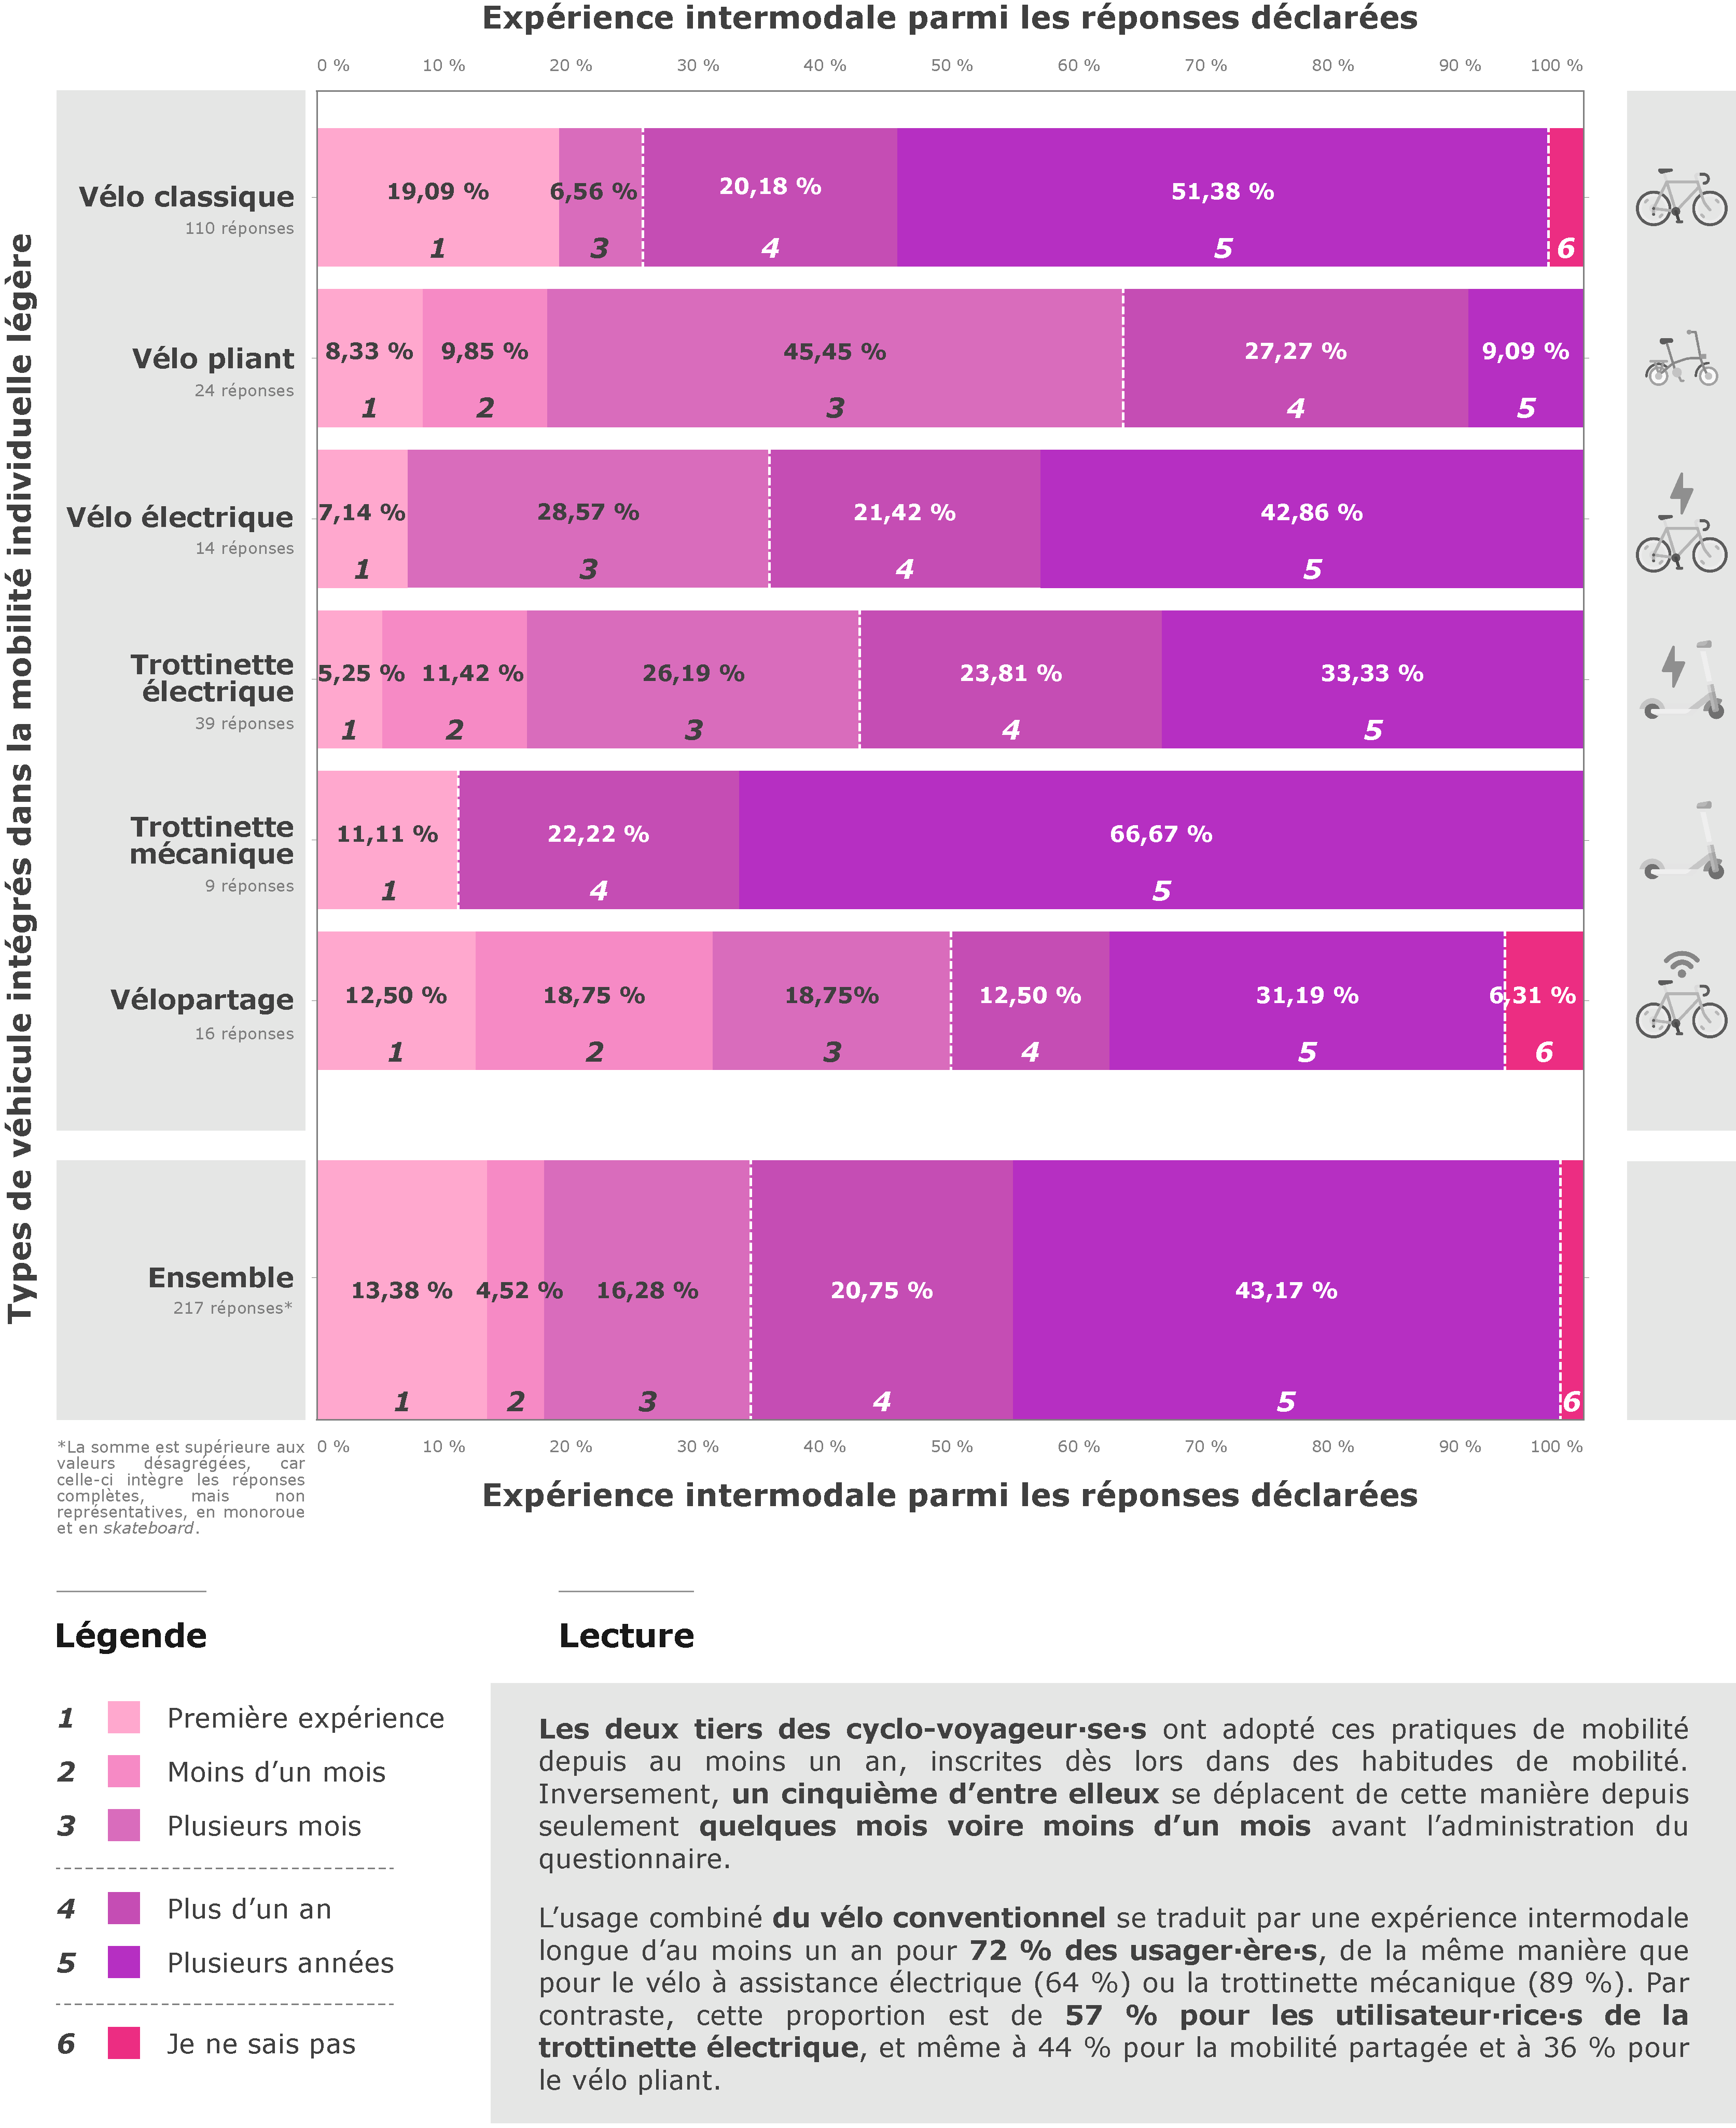
\includegraphics[width=1\columnwidth]{src/Figures/Chap-4/FR_Experience_intermodale.pdf}}
        \vspace{5pt}
        \begin{flushright}\scriptsize{
        Auteur~: \textcolor{blue}{Dylan Moinse (2023)}
        }\end{flushright}
    \end{figure}

    % Résultats par mode expérience intermodale
En affinant l'analyse de l'enquête par questionnaire aux différents véhicules constituant le corpus de la mobilité individuelle légère, il ressort que la trottinette mécanique et le vélo classique sont intégrés dans des configurations intermodales établies, avec plus des trois quarts des usager·ère·s les pratiquant depuis au moins un an. Par contraste, le \acrfull{VAE}, la \acrshort{TEP}, les systèmes de mobilité partagée ainsi que le vélo pliant montrent une adoption plus récente parmi les utilisateur·rice·s~: un tiers, voire la moitié d'entre elleux, ont commencé à les utiliser il y a moins de quelques mois. En conséquence, il est envisageable de déduire que le vélo conventionnel, d'une part, dépeint un mode de déplacement enraciné dans le paysage des pratiques intermodales, en étant traditionnellement associé au binôme vélo et transport public. D'autre part, les déclinaisons du vélo telles que le vélo pliant et, ou bien, électrique témoigne d'une recrudescence récente, en même temps que la \acrshort{TEP}, le \acrshort{VLS}, le \acrshort{VFF} et la \acrshort{TEFF} s'inscrivent dans une phase de croissance.%%Rédigé%%

    % Littérature expérience intermodale - vélo
La confrontation avec l'état des connaissances actuelles révèle que l'association du vélo avec le transport public suscite un intérêt notable, particulièrement entre 2005 et 2015. Ces pratiques intermodales présentent effectivement un potentiel de développement de leur part modale associé à un haut niveau de fidélisation des usager·ère·s dans le temps. Concernant le vélo classique, il est possible de noter une augmentation sensible de son usage en tant que mode de transfert vers ou depuis les gares néerlandaises, passant respectivement de 35~\% (pré-acheminement) et 10~\% (post-acheminement) en 2000 \textcolor{blue}{\autocite[73]{rietveld_accessibility_2000}}\index{Rietveld, Piet|pagebf} à 43~\% (pré-acheminement) et 14~\% (post-acheminement) en 2016 \textcolor{blue}{\autocite[456-457]{jonkeren_bicycle-train_2021}}\index{Jonkeren, Olaf|pagebf}\index{Kager, Roland|pagebf}\index{Harms, Lucas|pagebf}\index{te Brömmelstroet, Marco|pagebf}. Aux États-Unis, l'usage intermodal du vélo a progressé de 0,0~\% à 0,6~\% \textcolor{blue}{\autocite[101]{wang_bicycle-transit_2013}}\index{Wang, Rui|pagebf}\index{Liu, Chen|pagebf}, notamment dans les régions densément peuplées \textcolor{blue}{\autocite[107]{wang_bicycle-transit_2013}}\index{Wang, Rui|pagebf}\index{Liu, Chen|pagebf}. Ces données mettent en lumière la tendance à la hausse de la part modale du vélo, tout en soulignant l'existence d'une communauté de voyageur·se·s fidèles à ces pratiques intermodales. En effet, d'après l'étude de \textcolor{blue}{Christian} \textcolor{blue}{\textcite[18]{gioria_etude_2016}}\index{Gioria, Christian|pagebf}, 68~\% des usager·ère·s des consignes à vélo en gare en France utilisent ce service depuis plus d'un an, et 44~\% depuis plus de deux ans.%%Rédigé%%

    % Littérature expérience intermodale - micro-mobilité
La notion d'émergence, telle que décrite par \textcolor{blue}{\textcite[4]{kostrzewska_towards_2017}}\index{Kostrzewska, Małgorzata|pagebf}\index{Macikowski, Bartosz|pagebf}, suggère que l'intégration de la micro-mobilité est particulièrement prometteuse en matière de croissance d'adoption modale. En France, le rapport de l'\textcolor{blue}{\textcite[10]{ademe_observatoire_2017}}\index{ADEME@\textsl{ADEME}|pagebf} indique que le marché des modes de connexion aux nœuds est marqué par une pénétration importante des objets de \Guillemets{glisse urbaine}, dont la proportion a doublé entre 2014 et 2017, avec une part modale de la micro-mobilité atteignant 6~\%. Le Baromètre de la \acrfull{FP2M} confirme cette tendance, enregistrant une hausse de 34~\% des ventes de \acrshort{TEP} entre 2019 et 2020, représentant 640~000 unités vendues, contre seulement 100~000 en 2017 \textcolor{blue}{\autocite[2]{fp2m_barometre_2021}}\index{FP2M@\textsl{FP2M}|pagebf}\index{SML@\textsl{SML}|pagebf}. L'étude menée par l'agence \textcolor{blue}{\textcite[11]{smart_mobility_lab_usages_2020}}\index{Smart Mobility Lab@\textsl{Smart Mobility Lab}|pagebf} rapporte à son tour que 73~\% des utilisateur·rice·s monomodaux·les de la \acrshort{TEP} ont commencé à les utiliser il y a moins d'un an, dont 43~\% depuis moins de six mois. Cette évolution est d'autant plus notable qu'elle a été catalysée par la crise sanitaire de la COVID-19, qui a poussé 27~\% des personnes mobiles interrogé·e·s à modifier leurs habitudes de déplacement, adoptant pour 29~\% d'entre elleux un vélo ou un \acrshort{VAE} et pour 16~\% une option de micro-mobilité \textcolor{blue}{\autocite[16]{smart_mobility_lab_usages_2020}}\index{Smart Mobility Lab@\textsl{Smart Mobility Lab}|pagebf}.%%Rédigé%%

    % Transition
Il est essentiel, dans l'analyse des parts modales de la mobilité individuelle légère, de reconnaître les contextes urbains variés dans lesquels les gares sont implantées. La section suivante montre comment les caractéristiques spécifiques des zones urbaines et périurbaines influencent les pratiques intermodales, étant donné que les centres urbains, souvent mieux dotés en termes de services de mobilité, peuvent présenter des dynamiques de mobilité distinctes de celles des zones périurbaines, où les infrastructures de transport peuvent être moins diversifiées et les distances à parcourir plus importantes.%%Rédigé%%

    % 4.1.1.3.
    \needspace{1\baselineskip} % Réserve de l'espace
\subsubsection*{Un mode de déplacement pertinent à destination des gares de rabattement vers les pôles urbains
    \label{chap4:part-modale-gares-centre-periurbain}
    }

    % Introduction
Un exercice de mise en perspective des gares étudiées a été entreprise pour examiner les parts modales de la mobilité individuelle légère au sein des chaînes modales. Cette étude met en évidence une distribution spatiale caractéristique de ces pratiques intermodales, marquée par une concentration relative en fonction de la polarité du territoire dans lequel s'inscrit la gare. Cette sous-section vise alors à saisir les variations géographiques de tels déplacements intermodaux en soulignant l'importance des contextes urbains dans l'adoption et l'intégration de la mobilité légère au sein du réseau ferroviaire.%%Rédigé%%

    % Tableau Typologie des gares HdF
% Tableau Typologie des gares HdF
%%Rédigé%%
    \begin{table}[h!]
    \centering
    \renewcommand{\arraystretch}{1.5}
    \resizebox{\columnwidth}{!}{
    \begin{tabular}{p{0.27\columnwidth}p{0.13\columnwidth}p{0.60\columnwidth}}
        %\hline
    \rule{0pt}{15pt} \small{\textbf{\textcolor{blue}{Gare ou halte}}} & \small{\textbf{\textcolor{blue}{\acrshort{DRG}}}} & \small{\textbf{\textcolor{blue}{Contextualisation de la classe}}}\\
        \hline
\small{Creil} & \multirow{2}{*}{\small{Profil~\(a\)}} & \multirow{2}{*}{\small{\textsl{Gares de pôles régionaux}}}\\
    \small{Lille Flandres} & & \\
        \hdashline
\small{Armentières} & \multirow{3}{*}{\small{Profil~\(b\)}} & \multirow{3}{*}{\small{\textsl{Gares de pôles intermédiaires}}}\\
    \small{Béthune} & & \\
    \small{Dunkerque} & & \\
        \hdashline
\small{Le Poirier Université} & \multirow{4}{*}{\small{Profil~\(c\)}} & \multirow{4}{*}{\small{\textsl{Gares de rabattement vers les centralités urbaines}}}\\
\small{Lesquin} & & \\
\small{Lille CHR} & & \\
\small{Vis-à-Marles} & & \\
        \hline
        \end{tabular}}
    \caption{Réutilisation du référentiel \Guillemets{Segment DRG} appliqué aux neuf gares explorées dans la région Hauts-de-France.}
    \label{table-chap4:typologie-gares-hdf}
        \vspace{5pt}
        \begin{flushleft}\scriptsize{
        \textcolor{blue}{Lecture~:} ce tableau applique la typologie des segments aux neuf gares des Hauts-de-France explorées dans notre investigation, en les classant en trois profils distincts~: les profils~\(a\), \(b\) et \(c\).
        }\end{flushleft}
        \begin{flushright}\scriptsize
        Jeux de données~: \textcolor{blue}{\textcite{sncf_gares__connexions_gares_2024}}\index{SNCF Gares \& Connexions@\textsl{SNCF Gares \& Connexions}|pagebf}
        \\
        Auteur~: \textcolor{blue}{Dylan Moinse (2022)}
        \end{flushright}
        \end{table}%%Rédigé%%

    % Méthodologie
Notre démarche analytique, s'appuyant sur la typologie des gares établie par \textcolor{blue}{\textcite{sncf_gares__connexions_gares_2024}}\index{SNCF Gares \& Connexions@\textsl{SNCF Gares \& Connexions}|pagebf}, nous a permis d'affiner la caractérisation des parts modales de la mobilité individuelle légère en accès vers et depuis les différentes gares de la région. Les données recueillies au cours des séances d'observation quantitative ont été systématiquement rapprochées de la nomenclature des gares appelée \Guillemets{Segment \acrfull{DRG}}\footnote{
    Le référentiel \Guillemets{Segment \acrshort{DRG}} produit par la Direction de la Stratégie \textcolor{blue}{\textcite{sncf_gares__connexions_gares_2024}} définit trois catégories distinctes de gare, chacune reflétant une échelle d'intérêt et de fréquentation annuelle. Ce système de classification, qui repose principalement sur les volumes de fréquentation des gares, évalue 3~009 gares en France, dont 265 dans les Hauts-de-France. Ces profils sont répartis comme suit~: 
    \begin{customitemize}
    \item La classe~\(a\), désignant les \Guillemets{gares de voyageur·se·s d'intérêt national}, regroupe des gares à forte affluence, avec une fréquentation annuelle supérieure à 250 000 voyageur·se·s. Au niveau national, 102 gares sont classées dans cette catégorie, dont 8 se trouvent dans la région Hauts-de-France~;
    \item La classe~\(b\), correspondant aux \Guillemets{gares de voyageur·se·s d'intérêt régional}, inclut des gares ayant une fréquentation annuelle comprise entre 100 000 et 250 000 voyageur·se·s. Cette catégorie comprend 928 gares, avec 62 situées dans la région Hauts-de-France~;
    \item La classe~\(c\), regroupant les \Guillemets{gares de voyageur·se·s d'intérêt local}, est constituée de gares moins fréquentées, avec un flux annuel inférieur à 100 000 voyageur·se·s. Sur le plan national, 1~978 gares appartiennent à cette classe, avec 195 dans la région Hauts-de-France.
    \end{customitemize}
} (voir le \hyperref[table-chap4:typologie-gares-hdf]{tableau~\ref{table-chap4:typologie-gares-hdf}}, page~\pageref{table-chap4:typologie-gares-hdf}). L'exploitation de cette grille de lecture nous a conduits à donner un sens aux catégories issues du référentiel \Guillemets{Segment \acrshort{DRG}}, dans le contexte des neuf gares investies~:
    \begin{customitemize}
\item Les gares de pôles régionaux (\(a\)), situées au cœur des centralités urbaines, comprenant deux gares principales~;
\item Les gares de pôles intermédiaires (\(b\)), insérées dans des villes de taille moyenne, regroupant trois gares~;
\item Les gares de rabattement vers les centralités régionales (\(c\)), positionnées en périphérie des centres urbains, incluant quatre gares.
    \end{customitemize}%%Rédigé%%

    % Observation répartition géographique
L'analyse des parts modales de la mobilité individuelle légère embarquée dans différentes gares, selon leur profil, révèle une distribution hétérogène correspondant aux divers contextes urbains et périurbains des points d'arrêt examinés. Si les gares centrales telles que Lille Flandres et Creil concentrent un nombre significatif de cyclo-voyageur·se·s, avec 387 individus observés, représentant 37~\% du sous-échantillon, il est intéressant de noter que les territoires périurbains desservis par certaines des gares enquêtées présentent une part modale supérieure de l'usage de la mobilité individuelle légère relativement à leur fréquentation totale, sous réserve d'un niveau de service adéquat (voir l'\hyperref[fig-chap4:part-modale-urbain-periurbain]{illustration~\ref{fig-chap4:part-modale-urbain-periurbain}}, page~\pageref{fig-chap4:part-modale-urbain-periurbain}). En détail, la classe~\(a\), qui comprend les deux gares mentionnées, enregistre une proportion d'usager·ère·s intermodaux·les de 5~\% (sur 7~995 observations). En revanche, la classe~\(b\), qui inclut les gares d'Armentières, Béthune et Dunkerque, affiche une part modale de 7~\% (sur 5~826 observations). Cette tendance est encore plus marquée dans la classe~\(c\), qui regroupe les gares de Lille CHR, Le Poirier Université, Lesquin et Vis-à-Marles, avec une part modale de 14~\% (sur 1~617 observations).%%Rédigé%%

    % Observation répartition géographique détails modes 1
En affinant cette étude aux différentes composantes de la mobilité individuelle légère, nous pouvons relever une certaine constance parmi la distribution géographique des parts modales observées. L'\hyperref[fig-chap4:part-modale-urbain-periurbain]{illustration~\ref{fig-chap4:part-modale-urbain-periurbain}} (page~\pageref{fig-chap4:part-modale-urbain-periurbain}) met en lumière une croissance régulière des parts modales à mesure que nous progressons vers la troisième classe de la typologie, à l'exception de la halte de Vis-à-Marles. Ce phénomène indique une adoption privilégiée de la mobilité individuelle légère en tant que mode de transfert, dans les contextes périurbains~:
    \begin{customitemize}
\item Pour le vélo classique, une augmentation graduelle de la part modale est identifiée à travers les diverses classes, allant de 1,55~\% pour la classe~\(a\) (124 observations), à 2,18~\% pour la classe~\(b\) (127 observations) et à 4,83~\% pour la classe~\(c\) (78 observations)~;
\item Pour le vélo pliant, les parts modales sont de l'ordre de 0,56~\% pour la classe~\(a\) (45 observations), de 0,81~\% pour la classe~\(b\) (47 observations) et de 1,92~\% pour la classe~\(c\) (31 observations)~;
\item Pour la \acrshort{TEP}, les parts atteignent 2,26~\% pour la classe~\(a\) (171 observations), 3,16~\% pour la classe~\(b\) (184 observations) et 5,89~\% pour la classe~\(c\) (95 observations)~;
\item La trottinette mécanique montre une répartition de 0,43~\% pour la classe~\(a\) (34 observations), de 0,96~\% pour la classe~\(b\) (56 observations) et de 0,87~\% pour la classe~\(c\) (14 observations)~;
\item Pour les autres formes d'\acrshort{EDP}, les parts sont de 0,15~\% pour la classe~\(a\) (12 observations), de 0,24~\% pour la classe~\(b\) (14 observations) et de 0,12~\% pour la classe~\(c\) (2 observations).
    \end{customitemize}%%Rédigé%%

    % Observation répartition géographique détails modes 2
Cependant, certaines exceptions viennent nuancer cette tendance générale. Par exemple, la halte Lille CHR présente une part modale faible pour la trottinette mécanique. Cette particularité peut s'expliquer par les formes urbaines du territoire environnant, marquées par une faible porosité des tissus urbains et la présence de vastes parcelles telles que le \acrfull{CHU} de Lille, qui limite l'efficacité de ce mode de déplacement musculaire. De même, l'usage intermodal des \acrshort{EDP}, hormis la \acrshort{TEP} et qui incluent notamment le \textsl{skateboard}, le monoroue et le gyropode, ne semble pas correspondre à la tendance observée, probablement en raison d'un sous-échantillon trop restreint pour fournir une représentation statistique fiable.%%Rédigé%%

    % Figure Part modale périurbain
    \begin{figure}[h!]\vspace*{4pt}
        \caption{Un usage intermodal de la mobilité individuelle légère stimulé dans les territoires périurbains.}
        \label{fig-chap4:part-modale-urbain-periurbain}
        \centerline{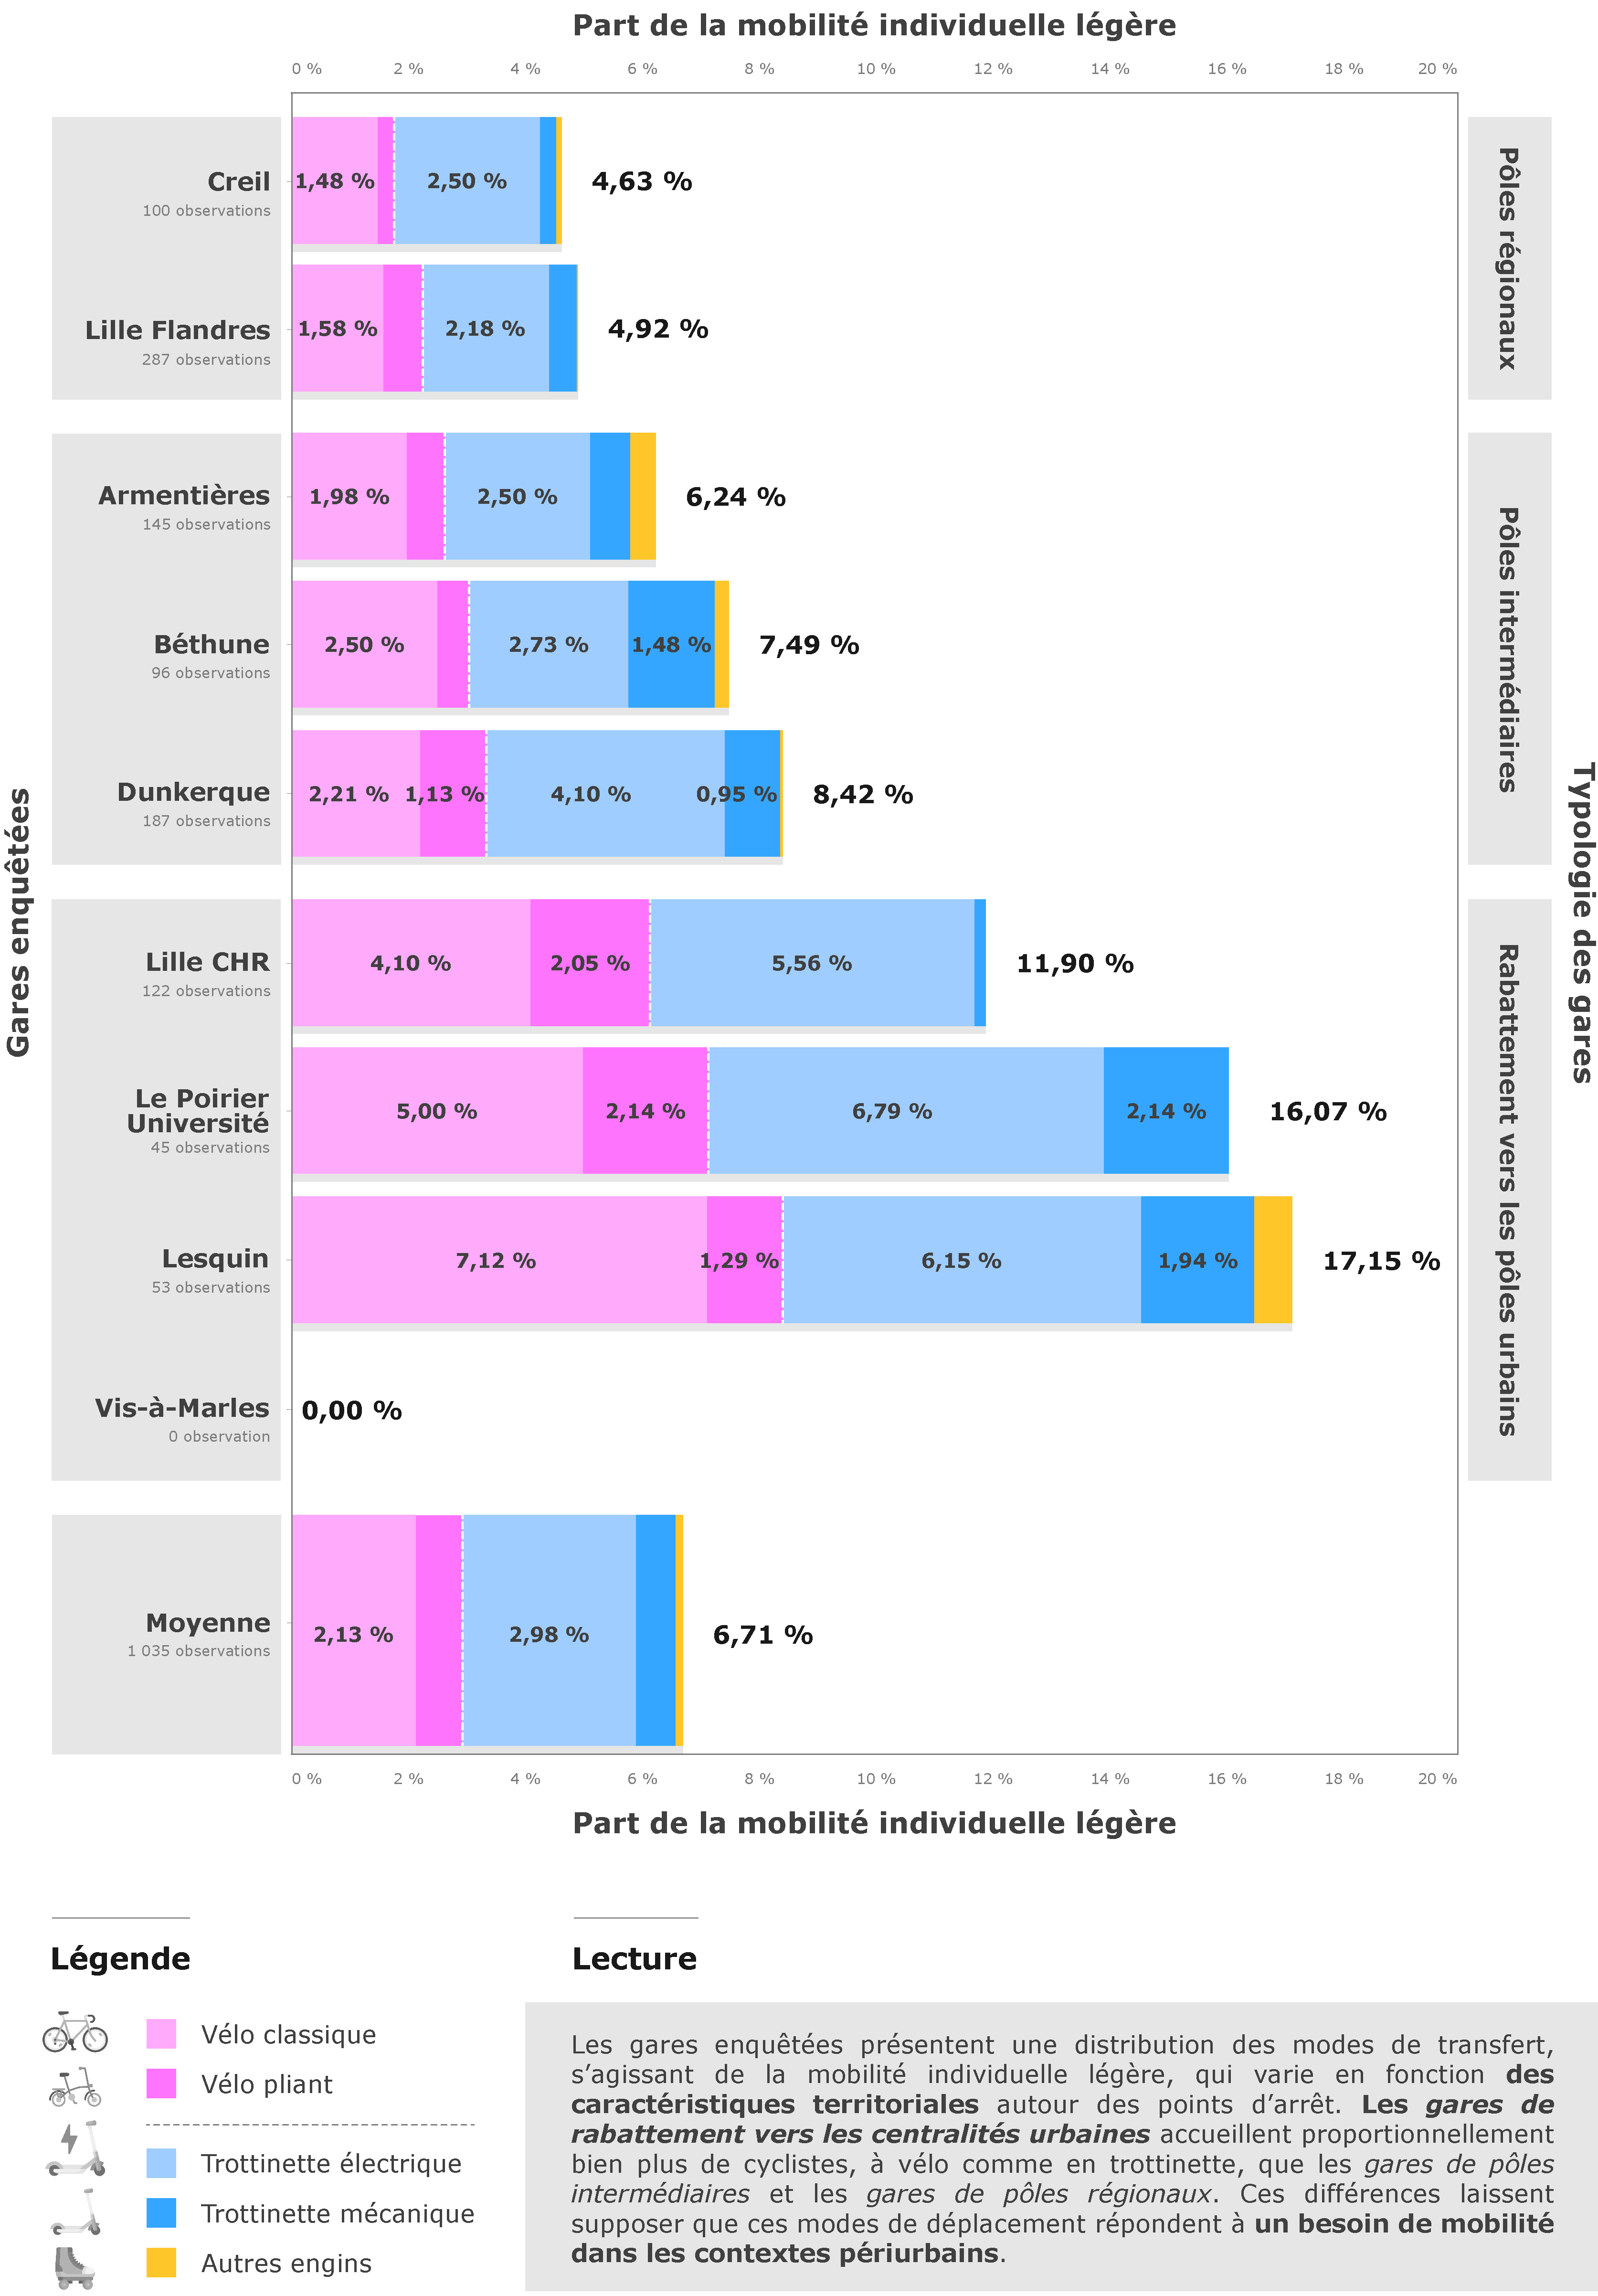
\includegraphics[width=1\columnwidth]{src/Figures/Chap-4/FR_Part_modale_MIL_gares.pdf}}
        \vspace{5pt}
        \begin{flushright}\scriptsize{
        Auteur~: \textcolor{blue}{Dylan Moinse (2023)}
        }\end{flushright}
    \end{figure}

    % Complément questionnaire flux OD
En exploitant les flux d'origine et de destination recueillis dans le questionnaire, cette analyse géostatistique cherche à approfondir les types de territoires que la mobilité individuelle légère combinée au transport public tend à connecter. Bien que l'observation quantitative souligne le rôle stratégique des gares de second rang dans le réseau ferroviaire régional, les réponses au questionnaire mettent en avant une densité importante de flux à destination des gares les plus fréquentées. L'évaluation spatiale des 99 déplacements intermodaux projetés dans les 9 gares étudiées révèle une majorité de trajets à vélo ou en micro-mobilité reliant une gare de classe~\(a\) à une gare de classe~\(b\), et inversement (60 flux). Viennent ensuite les déplacements entre gares de même type, notamment celles de classe~\(b\) (15 flux) et de classe~\(a\) (10 flux). Les interactions impliquant une gare de type~\(c\) sont moins fréquentes, avec peu de déplacements entre les gares~\(a\) et~\(c\) (8 flux), entre~\(b\) et~\(c\) (5 flux) et entre celles de classe~\(c\) (1 flux).%%Rédigé%%

    % Aires attraction
Cependant, en croisant les itinéraires en rabattement et en diffusion avec le zonage en \acrfull{AAV} produit par l'\textcolor{blue}{\textcite{insee_nouveau_2020}}\index{Insee@\textsl{Insee}|pagebf}\footnote{
    Le nouveau zonage en \acrfull{AAV} se compose de son pôle, avec sa commune la plus peuplée dénommée \Guillemets{commune-centre} et de sa zone d'attraction, la couronne \textcolor{blue}{\autocite{insee_nouveau_2020}}. Les couronnes regroupent les communes dont au moins 15~\% des actif·ve·s résident·e·s travaillent au sein des pôles ou des multipôles.
    Dans les Hauts-de-France, 65 aires d'attraction des villes sont recensées, dont 7 d'entre elles dans les régions voisines, et 2 autres s'étendant en Belgique, couvrant 83~\% des communes de la région et 95~\% de la population \textcolor{blue}{\autocite{insee_plus_2020}}.
}, nous pouvons déduire que, parmi les 78 déplacements intermodaux associés à une gare~\(a\), 42 d'entre eux impliquent un lieu d'origine et, ou bien, de destination qui s'inscrit dans une \Guillemets{couronne des grands pôles} et dans \Guillemets{des pôles moyens}. Ce constat suggère que, bien que l'adoption intermodale de la mobilité individuelle légère soit centrée sur les gares les plus attractives, la moitié de ces déplacements s'effectue, à destination, dans des zones moins densément peuplées.%%Rédigé%%

    % Littérature urbain - périurbain
Du point de vue de la documentation existante à ce sujet, il est admis dans une part importante de la littérature que les zones urbaines et centrales sont particulièrement favorables à l'adoption intermodale de la mobilité individuelle légère. Toutefois, notre recherche présente des résultats contraires quant aux parts modales analysées, apportant de nouvelles perspectives concernant le cas peu exploré de la micro-mobilité. Une enquête menée par le cabinet d'étude \textcolor{blue}{\textcite[18]{enov_enquete_2021}}\index{Enov@\textsl{Enov}|pagebf} dans six grandes gares françaises~–~Bercy, Gare de l'Est, Gare de Lyon, Lille Flandres, Lille Europe et Rouen Rive Droite~–~attribue une part modale moyenne de 2~\% pour le vélo et de 2~\% pour la micro-mobilité, qu'elle soit personnelle ou partagée. Ces résultats appuient l'hypothèse d'une répartition des modes de transfert moins visible de la mobilité individuelle légère dans les gares centrales. Dans une étude comparative entre les Pays-Bas, l'Allemagne et la Grande-Bretagne, \textcolor{blue}{\textcite[291]{martens_bicycle_2004}}\index{Martens, Karel|pagebf}, tout autant que \textcolor{blue}{\textcite[25]{halldorsdottir_home-end_2017}}\index{Halldórsdóttir, Katrín|pagebf}\index{Nielsen, Otto Anker|pagebf}\index{Prato, Carlo Giacomo|pagebf} dans le cas d'étude de Copenhague, ont démontré que l'association du vélo et des transports en commun est plus fréquente dans les zones périphériques. Le vélo y est perçu comme un élément stratégique pour étendre la portée des services ferroviaires dans les territoires périurbains et ruraux \textcolor{blue}{\autocite[86]{zuo_incorporating_2021}}\index{Zuo, Ting|pagebf}\index{Wei, Heng|pagebf}\index{Chen, Na|pagebf}. Ces observations suggèrent que l'utilisation de la mobilité individuelle légère en possession est favorisée dans un contexte périurbain \textcolor{blue}{\autocite[38]{stransky_periurbain_2019}}\index{Stransky, Vaclav|pagebf} et n'est donc pas réservée aux espaces centraux des agglomérations comme l'affirme une partie de la littérature.%%Rédigé%%

    % Transition
Ayant examiné le rôle stratégique du vélo et de la micro-mobilité dans les gares agissant comme points de rabattement vers les centres urbains, il est essentiel de reconnaître l'ampleur de leur adoption modale à travers les différents schémas de chaînage modal observés, notamment en matière d'emport et de stationnement des véhicules. À ce stade de l'analyse, il est légitime de questionner la fonction occupée par le vélo et la micro-mobilité dans la chaîne modale. Plus spécifiquement, nous sommes amené·e·s à déterminer si ces modes de déplacement sont principalement employés lors de l'étape de pré-acheminement ou de post-acheminement. La section suivante explore plus précisément les étapes de rabattement et de diffusion des pratiques intermodales spécifiques à chaque mode de déplacement.%%Rédigé%%

    % 4.1.1.4.
    \needspace{1\baselineskip} % Réserve de l'espace
\subsubsection*{Une adoption manifeste tant en rabattement qu'en diffusion
    \label{chap4:rabattement-diffusion}
    }

    % Questionnaire access/egress modes
Le questionnaire fournit un niveau de détail supplémentaire quant aux différentes phases constitutives de chaque déplacement intégrant la mobilité individuelle légère et le système de transport en commun. De manière générale, il apparaît que le vélo et la micro-mobilité, embarqués ou non, sont utilisés dans une proportion quasi identique pour les étapes de rabattement et de diffusion, atteignant respectivement 78~\% et 79~\% sur un total de 217 déplacements intermodaux, bien que des variations subsistent selon le type de véhicule concerné. Le \hyperref[table-chap4:part-modale-acces-diffusion-urbain-periurbain]{tableau~\ref{table-chap4:part-modale-acces-diffusion-urbain-periurbain}} (page~\pageref{table-chap4:part-modale-acces-diffusion-urbain-periurbain}) indique que les usager·ère·s du vélo classique et du \acrshort{VAE} privilégient particulièrement l'étape de pré-acheminement vers les nœuds de transport en commun (pour 110 et 14 déplacements). À l'inverse, le vélo pliant, la \acrshort{TEP}, la trottinette mécanique ainsi que les systèmes de vélo et de trottinette en libre-service tendent à favoriser davantage l'étape de post-acheminement à partir de ces nœuds (pour 24, 39, 9 et 16 déplacements). À titre comparatif, la marche combinée est nettement plus fréquemment utilisée lors du trajet en diffusion (pour 47 déplacements).%%Rédigé%%

    % Confrontation access/egress modes
Les analyses statistiques des comportements de mobilité des usager·ère·s dépeignent le vélo, à propulsion musculaire et électrique, comme un mode de déplacement approprié pour les \Guillemets{premiers kilomètres}, souvent couplé avec la marche en diffusion. En parallèle, le vélo pliant et la micro-mobilité, notamment représentée par la trottinette, redéfinissent le défi des \Guillemets{premiers et derniers kilomètres} en répondant aux besoins relatifs aux \Guillemets{derniers kilomètres}. Ces véhicules légers tendent à être fréquemment combinés avec l'usage de l'automobile, que ce soit en tant que conducteur·rice ou passager·ère, ainsi qu'avec les réseaux de transport en commun urbain pour le rabattement. Cette diversité de pratiques intermodales entre ces deux catégories de véhicules découle en partie des avantages comparatifs offerts par le vélo pliant et de la trottinette. En effet, leur compacité et leur légèreté confèrent à ces modes de déplacement une plus grande facilité d'embarquement dans d'autres véhicules, contexte dans lequel le recours au vélo classique ou électrique se révèle moins pratique.%%Rédigé%%

    % Tableau Part modale intermodale - modes de transfert
% Tableau Part modale intermodale - modes de transfert
%%Rédigé%%
    \begin{table}[h!]
    \centering
    \renewcommand{\arraystretch}{1.5}
    \resizebox{\columnwidth}{!}{
    \begin{tabular}{p{0.4\columnwidth}p{0.18\columnwidth}p{0.14\columnwidth}p{0.14\columnwidth}p{0.14\columnwidth}}
        %\hline
    \rule{0pt}{15pt} \small{\textbf{\textcolor{blue}{Type de véhicule}}} & \small{\textbf{\textcolor{blue}{Rabattement}}} & \small{\textbf{\textcolor{blue}{Couronne}}} & \small{\textbf{\textcolor{blue}{Diffusion}}} & \small{\textbf{\textcolor{blue}{Couronne}}}\\
        \hline
\small{\textbf{Tous types de mobilité individuelle légère confondus}} & \multirow{1.5}{*}{\small{\textbf{78,34~\%}}} & \multirow{1.5}{*}{\small{\textbf{31,86~\%}}} & \multirow{1.5}{*}{\small{\textbf{78,80~\%}}} & \multirow{1.5}{*}{\small{\textbf{20,59~\%}}}\\
        \hdashline
\small{Vélo conventionnel} & \small{80,51~\%} & \small{34,58~\%} & \small{65,25~\%} & \small{20,56~\%}\\
\small{Vélo électrique (\acrshort{VAE})} & \small{76,92~\%} & \small{60,00~\%} & \small{61,54~\%} & \small{20,00~\%}\\
\small{Vélo pliant} & \small{80,95~\%} & \small{21,74~\%} & \small{100,00~\%} & \small{26,09~\%}\\
\small{Trottinette électrique (\acrshort{TEP})} & \small{80,43~\%} & \small{38,46~\%} & \small{100,00~\%} & \small{25,64~\%}\\
\small{Trottinette mécanique} & \small{77,78~\%} & \small{20,00~\%} & \small{100,00~\%} & \small{20,00~\%}\\
\small{Mobilité partagée} & \small{40,00~\%} & \small{0,00~\%} & \small{70,00~\%} & \small{0,00~\%}\\
        \hdashline
\small{Marche combinée} & \small{36,17~\%} & \small{17,24~\%} & \small{63,83~\%} & \small{10,34~\%}\\
        \hline
        \end{tabular}}
    \caption{Usage intermodal de la mobilité individuelle légère en rabattement depuis et en diffusion vers les territoires périurbains.}
    \label{table-chap4:part-modale-acces-diffusion-urbain-periurbain}
        \vspace{5pt}
        \begin{flushleft}\scriptsize{
        \textcolor{blue}{Lecture~:} parmi les utilisateur·rice·s combinant la mobilité individuelle légère avec le système de transport en commun et ayant déclaré leur déplacement dans le cadre du questionnaire, 78~\% d'entre elleux circulent avec un véhicule léger en pré-acheminement et 32~\% ont pour origine un territoire périurbain, tandis que 79~\% y ont recours en post-acheminement et 21~\% ont pour destination un territoire périurbain.
        }\end{flushleft}
        \begin{flushright}\scriptsize
        Auteur~: \textcolor{blue}{Dylan Moinse (2023)}
        \end{flushright}
        \end{table}%%Rédigé%%

    % Access/egress et urbain/périurbain
Contrairement au triptyque traditionnel composé du vélo, des transports en commun et de la marche combinée, la \acrshort{TEP} et le vélo pliant offrent à leurs utilisateur·rice·s la possibilité d'atteindre des destinations plus éloignées une fois sorti·e·s de la station de transport en commun. Cette capacité étend théoriquement l'accessibilité à certains territoires périurbains, comme en témoigne le \hyperref[table-chap4:part-modale-acces-diffusion-urbain-periurbain]{tableau~\ref{table-chap4:part-modale-acces-diffusion-urbain-periurbain}} (page~\pageref{table-chap4:part-modale-acces-diffusion-urbain-periurbain}). En effet, 38~\% des voyageur·se·s se déplaçant en \acrshort{TEP} et 26~\% des voyageur·se·s en vélo pliant commencent ou terminent leur déplacement en milieu périurbain. Ces proportions sont comparables à celles observées pour le vélo classique pour les \Guillemets{premiers kilomètres}, mais les dépassent lors de la phase de diffusion.%%Rédigé%%

    % Discussion
Cette sous-section a démontré que la mobilité individuelle légère est fréquemment sollicitée comme mode de transfert, servant ainsi à compléter efficacement le réseau de transport en commun. L'essor de la \acrshort{TEP}, du vélo pliant à assistance électrique, ainsi que des services de vélo et de micro-mobilité partagés, semble avoir significativement stimulé sa part modale. L'usage intermodal de la mobilité individuelle légère sert aussi bien pour le rabattement que pour la diffusion, avec une adoption croissante des véhicules pliants. Bien que le nombre d'usager·ère·s soit plus important dans les centres urbains, leur présence est proportionnellement plus marquée dans les territoires périurbains desservis par des gares offrant un certain niveau de service. De plus, il a été observé que ces modes de déplacement sont principalement regroupés dans les gares les plus centrales, mais que ceux-ci viennent ensuite communiquer avec des territoires plus éloignés des pôles urbains. Cette observation suggère que les cyclo-voyageur·se·s sont disposé·e·s à favoriser une connexion à des gares bien desservies et à parcourir de plus longues distances pour atteindre les zones périurbaines. Cette hypothèse sera explorée dans la \hyperref[chap5:detours-pauses-optimisation]{section consacrée à l'optimisation du mouvement par le détour} (page~\pageref{chap5:detours-pauses-optimisation}) dans le \hyperref[chap5:titre]{chapitre~5} (page~\pageref{chap5:titre}).%%Rédigé%%

    % Transition
L'émergence de nouvelles formes de mobilité, conjuguée au retour du vélo et composant la mobilité individuelle légère, semblent accroître significativement la part des voyageur·se·s intermodaux·les en gare, avec une augmentation estimée entre un quart et la moitié de la proportion initiale. Toutefois, cette interprétation statistique mérite d'être vérifiée, notamment en examinant l'éventuel effet de substitution modale induit par ces véhicules récemment adoptés. La question sous-jacente est de déterminer dans quelle mesure la micro-mobilité se substitue simplement aux pratiques intermodales préexistantes, où le vélo était combiné avec le rail, ou bien si celle-ci entraîne réellement un accroissement net du nombre d'usager·ère·s optant pour des combinaisons intermodales. Plus largement, la sous-section suivante vise à mieux comprendre les comportements de mobilité des cyclo-voyageur·se·s.%%Rédigé%%

    % 4.2.1.
    \needspace{1\baselineskip} % Réserve de l'espace
\subsection{Comportements de mobilité
    \label{chap4:comportements-mobilite}
    }

    % Introduction
Après validation de la première hypothèse affirmant que l’intégration de la mobilité individuelle légère aux réseaux de transport en commun est en phase d'émergence, nous nous orientons vers une exploration des interactions avec les services ferroviaires. Il s’agit désormais d’analyser l’impact et les opportunités que représentent ces pratiques intermodales pour les systèmes de transport public. L'exploitation des données recueillies au moyen du questionnaire administré en ligne a permis de doter la mesure de la pratique intermodale en gare d'une première caractérisation globale des comportements de mobilité. À cet égard, une section spécifique du questionnaire a été dédiée à l'examen des habitudes des répondant·e·s quant à la fréquence d'utilisation combinée de ces modes de déplacement, de même qu'aux motifs de leurs déplacements, à leur expérience intermodale et aux motivations sous-jacentes à une telle pratique de mobilité.%%Rédigé%%

    % 4.2.1.1.
    \needspace{1\baselineskip} % Réserve de l'espace
\subsubsection*{Des déplacements intermodaux inscrits dans les mobilités quotidiennes
    \label{chap4:frequence-motif-experience}
    }

    % Fréquence - général
L'usage intermodal de la mobilité individuelle légère semble majoritairement servir à des déplacements fréquents, de type pendulaires, comme le laisse voir l'\hyperref[fig-chap4:frequence-modes]{illustration~\ref{fig-chap4:frequence-modes}} (page~\pageref{fig-chap4:frequence-modes}). Sur 100 voyageur·se·s intermodaux·les faisant appel à la mobilité individuelle légère, 53 adoptent cette pratique de manière quasi quotidienne (\Guillemets{plus d'un déplacement quotidien} ou \Guillemets{plusieurs déplacements par semaine}, 116 réponses) et 8 de manière régulière (\Guillemets{un déplacement par semaine}, 17  réponses). Les autres segments de fréquence d'utilisation se répartissent de la manière suivante~: 13 d'entre elleux l'utilisent occasionnellement (\Guillemets{plusieurs fois par mois}~ou \Guillemets{au moins une fois par mois}, 28  réponses), 12 autres maintiennent une fréquence rare (\Guillemets{plusieurs fois par an}~ou \Guillemets{au moins une fois par an}, 26  réponses) et 13 répondant·e·s signalent que leur participation à l'enquête coïncide avec leur première expérience intermodale (\Guillemets{première utilisation}, 28  réponses).%%Rédigé%%

    % Figure fréquence modes
    \begin{figure}[h!]\vspace*{4pt}
        \caption{Fréquence d'usage intermodal de la mobilité individuelle légère.}
        \label{fig-chap4:frequence-modes}
        \centerline{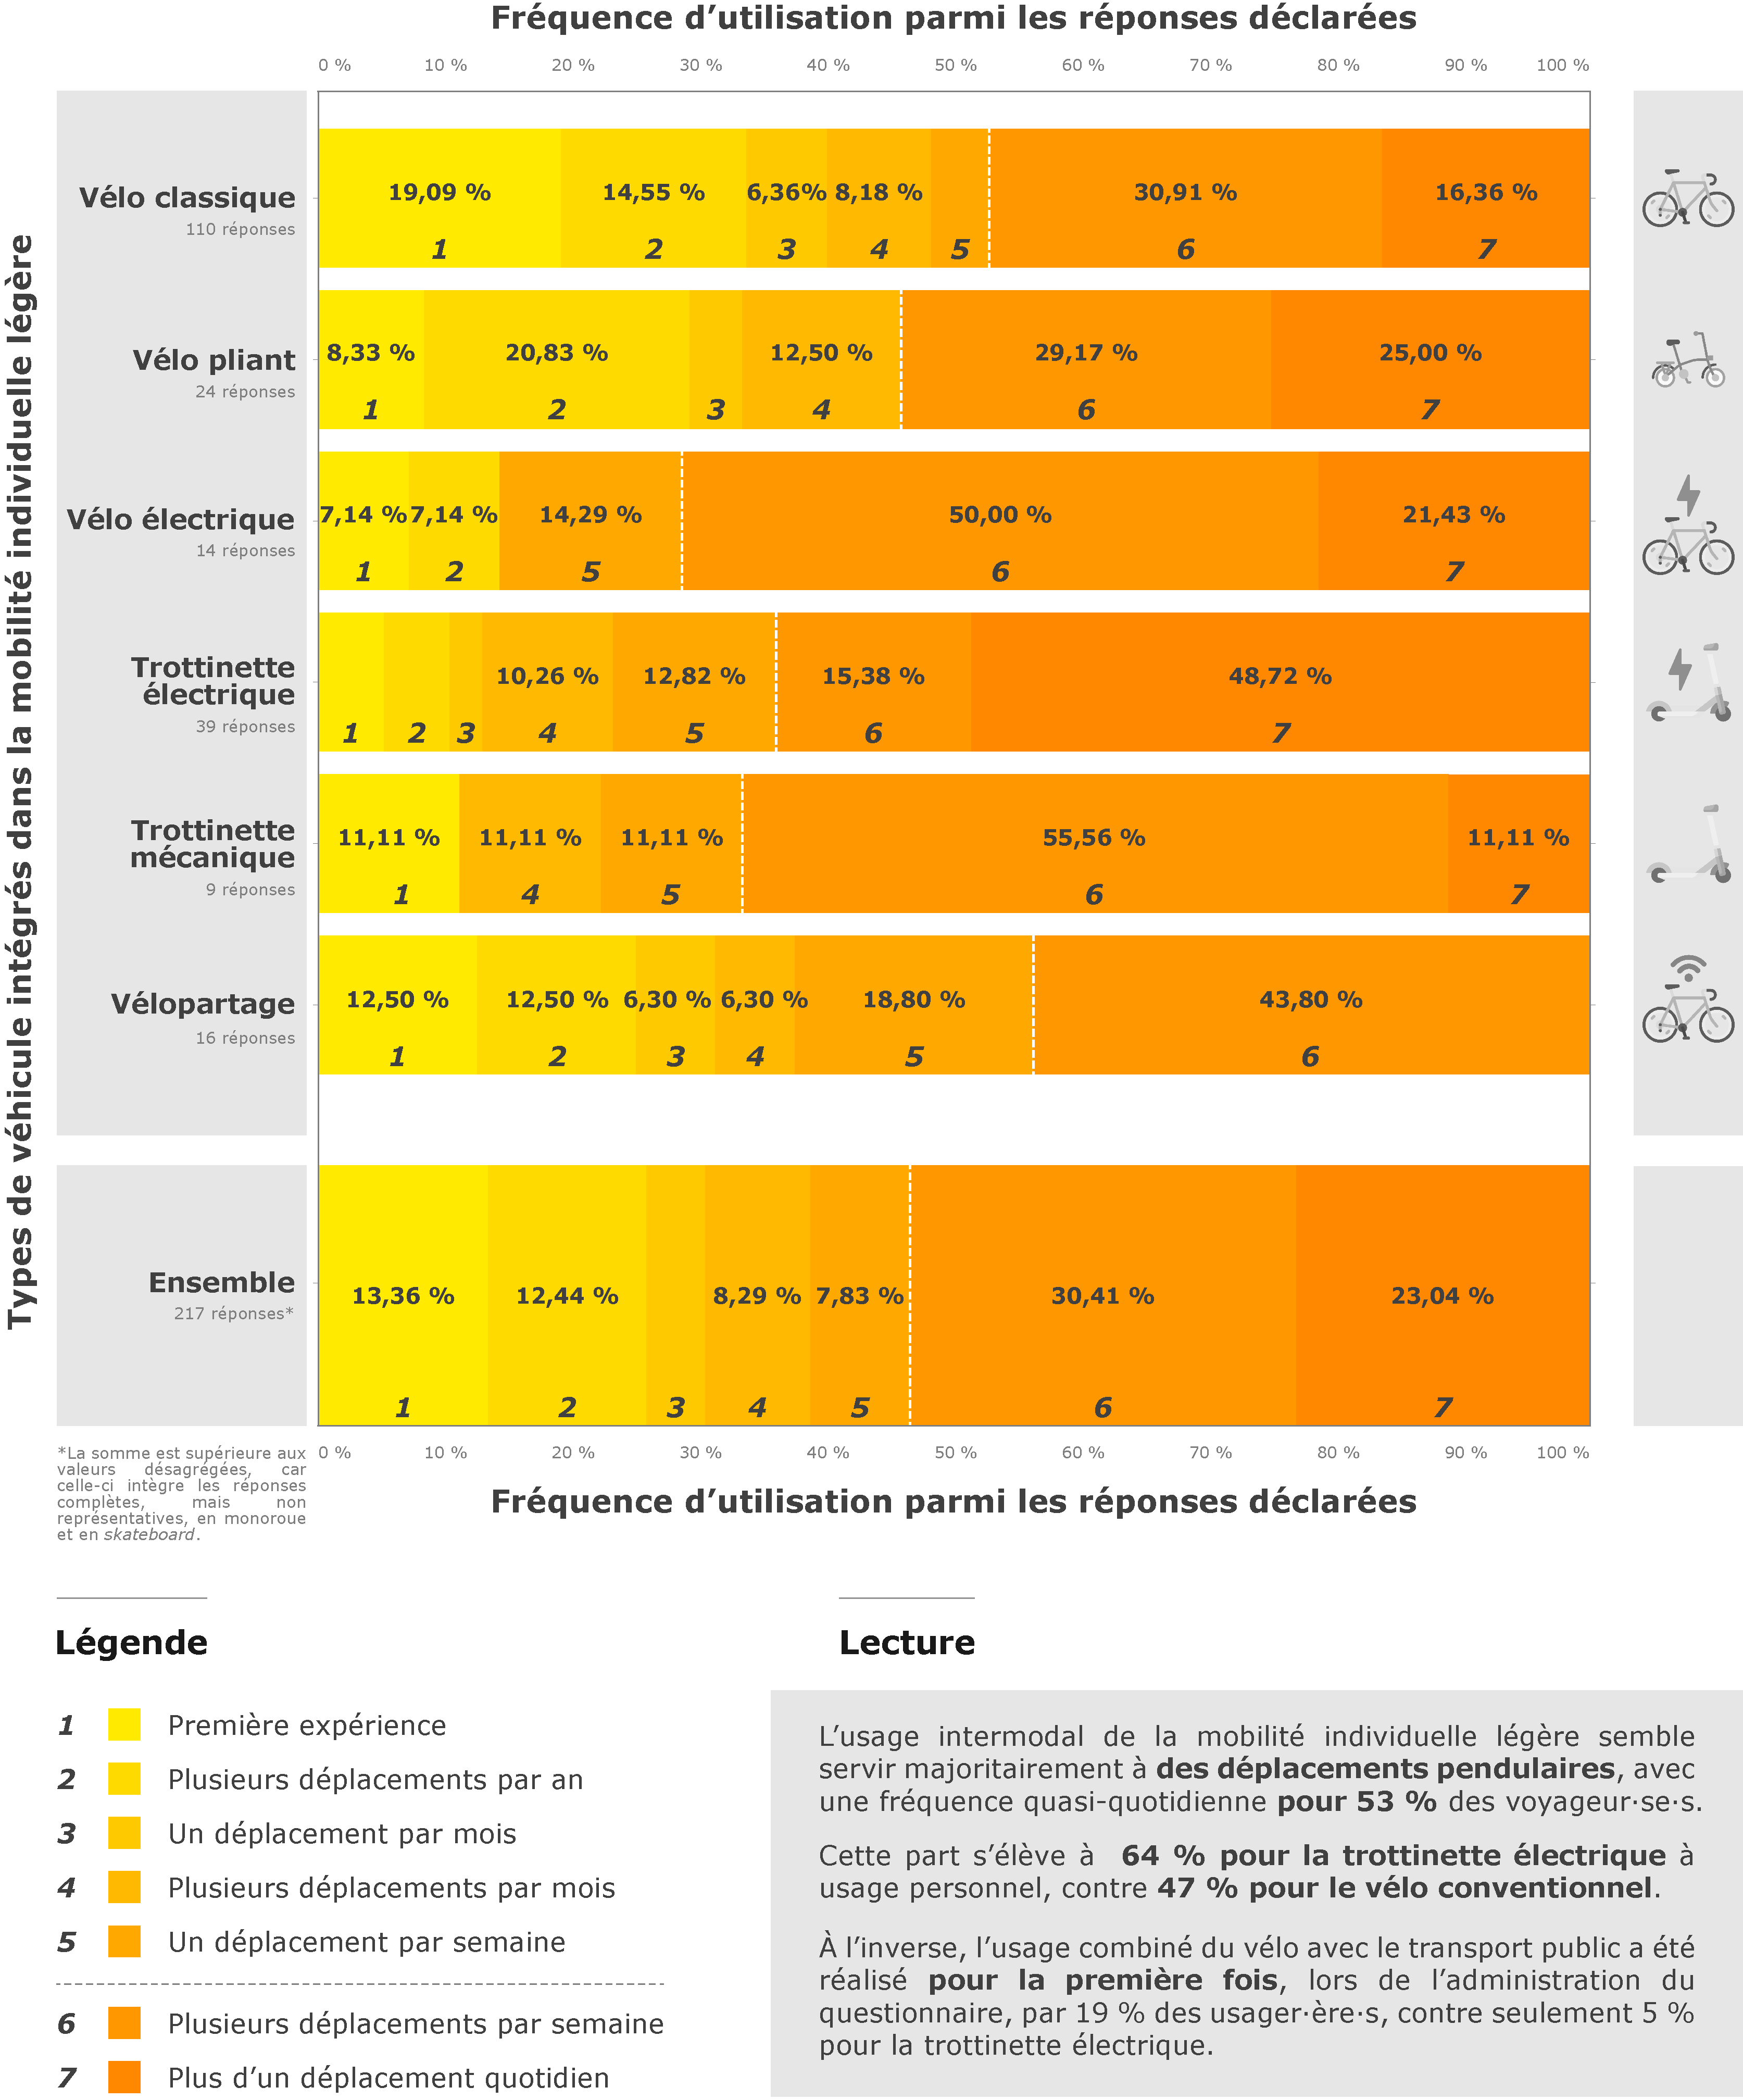
\includegraphics[width=1\columnwidth]{src/Figures/Chap-4/FR_Frequence.pdf}}
        \vspace{5pt}
        \begin{flushright}\scriptsize{
        Auteur~: \textcolor{blue}{Dylan Moinse (2023)}
        }\end{flushright}
    \end{figure}

    % Fréquence - modes
L'intégration de la mobilité individuelle légère au sein du système de transport en commun est caractérisée par une utilisation presque quotidienne pour la majorité des modes de déplacement étudiés (voir l'\hyperref[fig-chap4:frequence-modes]{illustration~\ref{fig-chap4:frequence-modes}}, page~\pageref{fig-chap4:frequence-modes}), à l'exception du \acrshort{VLS}, du \acrshort{VFF} et de la \acrshort{TEFF}, pour lesquels la part est de 44~\% (7 réponses) ainsi que du vélo classique, à 47~\% (52 réponses). \textsl{A contrario}, la \acrshort{TEP} enregistre une fréquence d'utilisation quasi quotidienne de 64~\% (25 réponses), la trottinette mécanique de 67~\% (6 réponses) et le \acrshort{VAE} de 71~\% (10 réponses).%%Rédigé%%

    % Motifs - général
Cette observation statistique relative à la fréquence d'utilisation intermodale de la mobilité individuelle légère est complétée par une analyse des motifs de déplacement (voir l'\hyperref[fig-chap4:motifs-modes]{illustration~\ref{fig-chap4:motifs-modes}}, page~\pageref{fig-chap4:motifs-modes}). Ce niveau d'information supplémentaire permet d’apporter des clés de compréhension de la fréquence d’utilisation des diverses combinaisons modales par les usager·ère·s. À cet égard, les résultats révèlent que la grande majorité des personnes ayant participé au questionnaire sont des navetteur·se·s régulier·ère·s, relevant de la mobilité quotidienne. Parmi 100 voyageur·se·s intermodaux·les, 76 y ont principalement recours pour se rendre à leur lieu de travail ou d'études (165 réponses). Suivent les activités de loisirs et les achats, motifs évoqués par 19 participant·e·s (41 réponses), ainsi que la promenade ou le tourisme, cités par 5 d'entre elleux (11 réponses).%%Rédigé%%

    % Figure fréquence modes
    \begin{figure}[h!]\vspace*{4pt}
        \caption{Distribution des premiers motifs de déplacement déclarés.}
        \label{fig-chap4:motifs-modes}
        \centerline{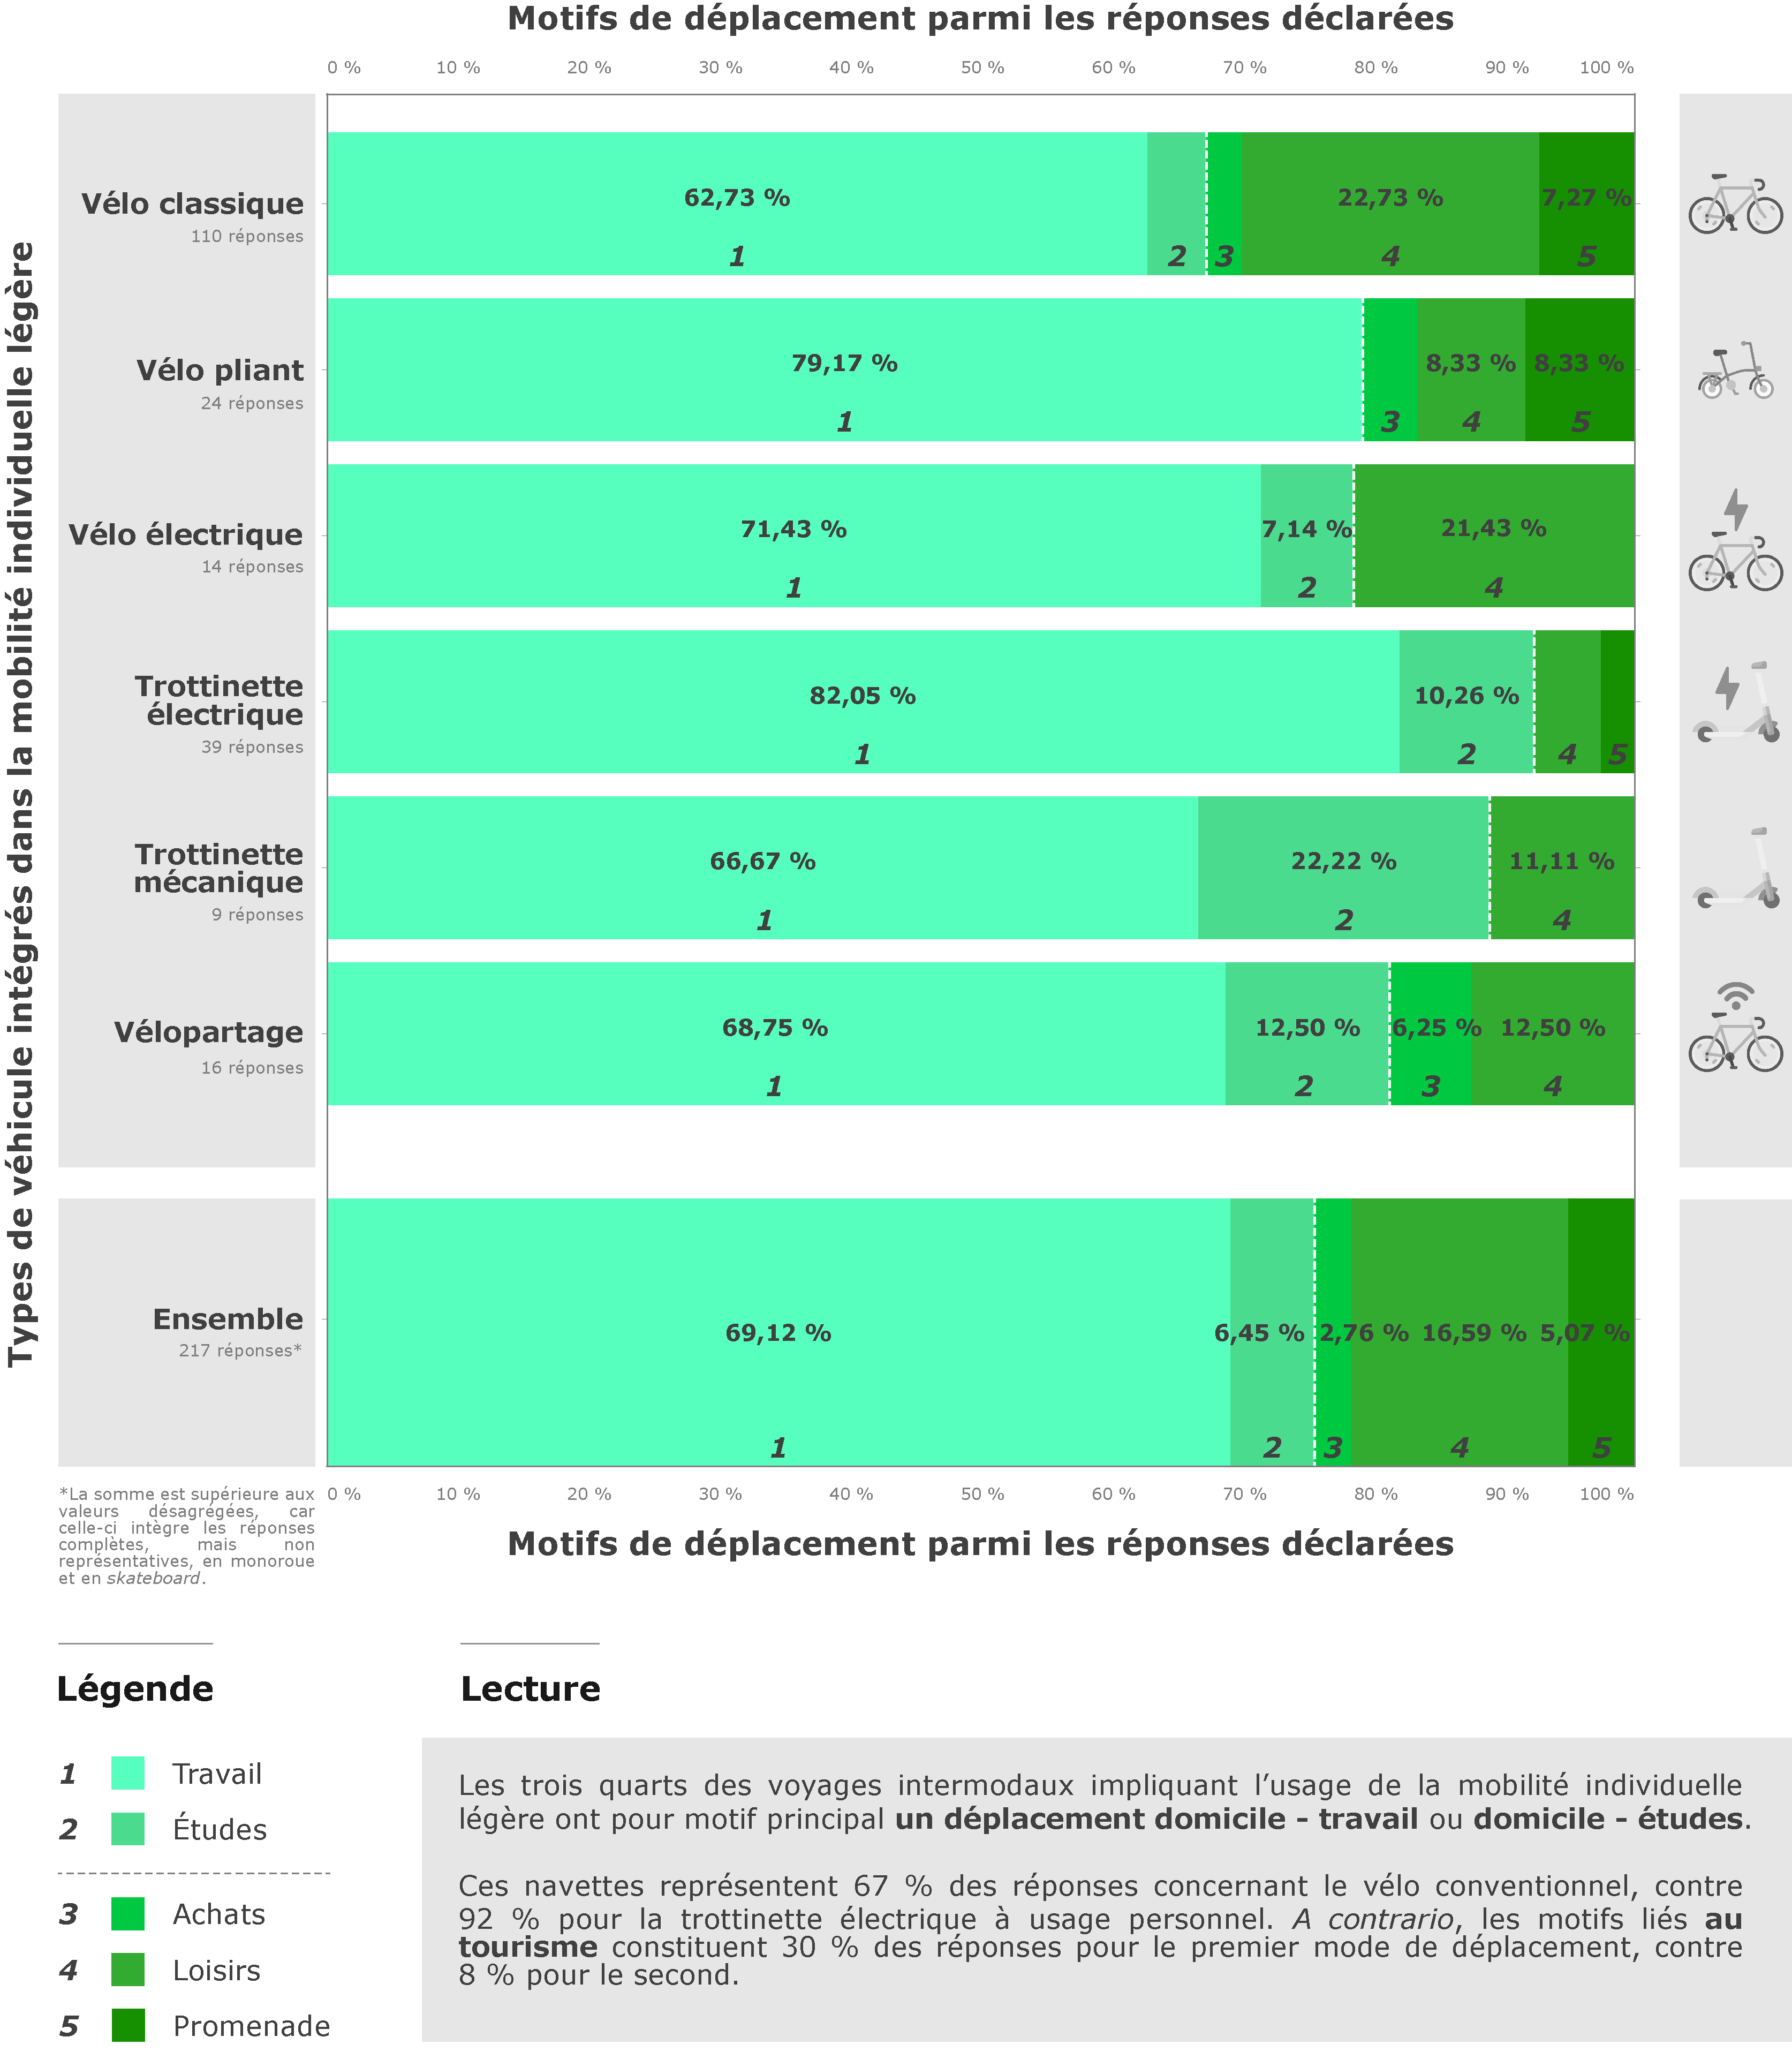
\includegraphics[width=1\columnwidth]{src/Figures/Chap-4/FR_Motifs.pdf}}
        \vspace{5pt}
        \begin{flushright}\scriptsize{
        Auteur~: \textcolor{blue}{Dylan Moinse (2023)}
        }\end{flushright}
    \end{figure}

    % Fréquence + motifs - général
Afin de mieux saisir les interactions entre la fréquence d'usage et le motif de déplacement, nous avons veillé à croiser ces deux variables. Il ressort de cette analyse que 69~\% des navetteur·se·s sont des utilisateur·rice·s quotidien·ne·s. En contraste, parmi les voyageur·se·s dont les déplacements sont motivés par les loisirs ou les achats, 52~\% d'entre elleux ont rarement recours à ces pratiques intermodales, alors que 31~\% d'entre elleux se sont déplacé·e·s de cette manière pour la première fois. Cette différenciation marque une tendance claire quant à la régularité d'utilisation selon la finalité du déplacement.%%Rédigé%%

    % Motifs - modes
Une nette distinction se manifeste dans la répartition des motifs de déplacement selon le type de véhicule choisi. Les objets de \Guillemets{glisse urbaine} sont proportionnellement plus sollicités à des fins pendulaires que le vélo, et notamment le vélo classique dont l'usage est plus diversifié (voir l'\hyperref[fig-chap4:motifs-modes]{illustration~\ref{fig-chap4:motifs-modes}}, page~\pageref{fig-chap4:motifs-modes}). Ainsi, 67~\% des utilisateur·rice·s du vélo classique recourent à ces pratiques intermodales pour réaliser des déplacements de nature pendulaire, tandis que cette part s'élève à 79~\% pour le \acrshort{VAE}, à 79~\% pour le vélo pliant, à 81~\% à la fois pour le \acrshort{VLS}, le \acrshort{VFF} et la \acrshort{TEFF}, à 89~\% pour la trottinette mécanique et à 92~\% pour la \acrshort{TEP}. Cette variation peut s'expliquer par une utilisation relativement plus importante du vélo par les cyclo-voyageur·se·s pour compléter leurs parcours touristiques. Nous observons néanmoins que la fréquence d'utilisation quotidienne de ces combinaisons modales ne correspond pas exactement à la répartition des motifs de déplacement déclarés ni aux profils des usager·ère·s, qui sont presque tou·te·s des actif·ve·s à temps plein. Même en tenant compte du fait que le télétravail peut réduire la fréquence quotidienne d'utilisation intermodale de la mobilité individuelle légère parmi les individus pouvant en bénéficier, il semble que certain·e·s de ces usager·ère·s tendent à alterner entre les pratiques intermodales étudiées et d'autres modes de déplacement au cours de la même semaine.%%Rédigé%%

    % Motifs par kilomètres parcourus
Une étape supplémentaire de l'analyse statistique du questionnaire examine la répartition des déplacements intermodaux selon différents motifs et leur proportion relative en termes de distances spatiales et temporelles. Les motifs de déplacement liés aux achats, aux démarches administratives, aux visites sociales et aux promenades, bien qu'ils représentent une part moins significative des usages intermodaux en lien avec la mobilité individuelle légère, se distinguent par des distances spatio-temporelles plus étendues comparées aux activités professionnelles ou scolaires. Alors que les déplacements intermodaux pour le travail constituent 69~\% des motifs déclarés, ces navettes ne représentent que 55~\% des kilomètres parcourus (\textsl{Vehicle Miles Traveled}, VMT) et 54~\% du temps de déplacement total. Cet écart est encore plus marqué pour les déplacements domicile-études, qui, en représentant 6~\% des réponses, ne totalisent que 4~\% des distances spatiales et 4~\% des distances temps. En contraste, les activités de loisir, qui comptent pour 17~\% des retours du questionnaire, occupent 38~\% des kilomètres et 38~\% du temps déclarés. Ces données appuient l'importance de considérer non seulement la finalité des déplacements associée aux diverses activités, mais également leur fréquence, en relation avec les budgets spatiaux et temporels alloués.%%Rédigé%%

    % Littérature fréquence et motifs
Les déplacements intermodaux, combinant l'utilisation de la mobilité individuelle légère et du train, sont majoritairement caractérisés par leur nature pendulaire. Notre observation empirique rejoint les connaissances actuelles sur les déplacements combinant transport public, vélo et micro-mobilité. La littérature scientifique indique que généralement, ces navetteur·se·s recourent à ces modes de déplacement combinés plus de quatre à cinq fois par semaine \textcolor{blue}{\autocite[104]{flamm_public_2014}}\index{Flamm, Bradley~J.|pagebf}\index{Rivasplata, Charles~R.|pagebf} pour des motifs professionnels ou scolaires, incluant tant l'usage du vélo à usage personnel \textcolor{blue}{\autocites[288]{martens_bicycle_2004}[16]{la_paix_puello_train_2016}[78]{oostendorp_combining_2018}[15]{shelat_analysing_2018}[8]{jonkeren_bicycle_2021}[184]{moinse_intermodal_2022}}\index{Shelat, Sanmay|pagebf}\index{Huisman, Raymond|pagebf}\index{Oort, Niels van|pagebf}\index{La Paix Puello, Lissy|pagebf}\index{Geurs, Karst~T.|pagebf}\index{Jonkeren, Olaf|pagebf}\index{Kager, Roland|pagebf}\index{Oostendorp, Rebekka|pagebf}\index{Gebhardt, Laura|pagebf}\index{Martens, Karel|pagebf}\index{Moinse, Dylan|pagebf}\index{Goudeau, Matthieu|pagebf}\index{L'Hostis, Alain|pagebf}\index{Leysens, Thomas|pagebf}, que de la \acrshort{TEP} \textcolor{blue}{\autocites[184]{moinse_intermodal_2022}[62]{rabaud_quand_2022}}\index{Moinse, Dylan|pagebf}\index{Goudeau, Matthieu|pagebf}\index{L'Hostis, Alain|pagebf}\index{Leysens, Thomas|pagebf}\index{Rabaud, Mathieu|pagebf}\index{Richer, Cyprien|pagebf}, ainsi que de services de mobilité \textcolor{blue}{\autocites[68]{ma_understanding_2018}[10]{gu_measuring_2019}[18]{lin_analysis_2019}[394]{bocker_bike_2020}[10]{fan_dockless_2020}[11]{wang_spatiotemporal_2020}[10-11]{heumann_spatiotemporal_2021}[8]{kim_analysis_2021}[8]{qiu_interplay_2021}[8]{yu_understanding_2021}[8]{yu_policy_2021}}\index{Böcker, Lars|pagebf}\index{Anderson, Ellinor|pagebf}\index{Uteng, Tanu Priya|pagebf}\index{Throndsen, Torstein|pagebf}\index{Ma, Xinwei|pagebf}\index{Ji, Yanjie|pagebf}\index{Yang, Mingyuan|pagebf}\index{Jin, Yuchuan|pagebf}\index{Tan, Xu|pagebf}\index{Gu, Tianqi|pagebf}\index{Yu, Qing|pagebf}\index{Li, Weifeng|pagebf}\index{Yang, Dongyuan|pagebf}\index{Xie, Yingkun|pagebf}\index{Kim, Minjun|pagebf}\index{Cho, Gi-Hyoung|pagebf}\index{Yu, Senbin|pagebf}\index{Liu, Gehui|pagebf}\index{Yin, Congru|pagebf}\index{Lin, Diao|pagebf}\index{Zhang, Yongping|pagebf}\index{Zhu, Ruoxin|pagebf}\index{Meng, Liqiu|pagebf}\index{Qiu, Waishan|pagebf}\index{Chang, Hector|pagebf}\index{Heumann, Maximilian|pagebf}\index{Kraschewski, Tobias|pagebf}\index{Brauner, Tim|pagebf}\index{Tilch, Lukas|pagebf}\index{Breitner, Michael|pagebf}.%%Rédigé%%

    % Transition
Ayant analysé les pratiques intermodales et dégagé les principales tendances relatives à la fréquence et aux motifs des déplacements, il convient désormais de se pencher sur les facteurs sous-jacents qui guident ces choix modaux. La section suivante éclaire sur la hiérarchisation des raisons qui motivent l'adoption de ces combinaisons modales.%%Rédigé%%

    % 4.2.1.2.
    \needspace{1\baselineskip} % Réserve de l'espace
\subsubsection*{Hiérarchisation des raisons de l'adoption modale~: \textsl{portée}, \textsl{flexibilité} et \textsl{écologie}
    \label{chap4:raisons-adoption}
    }

    % Raisons adoption - général
Interrogé·e·s sur les principaux facteurs ayant motivé leur choix d'adopter ces pratiques intermodales, les participant·e·s ont évalué diverses dimensions à partir d'un classement. Ces aspects incluent certains avantages comparatifs de ces chaînages modaux, tels que l'optimisation spatio-temporelle de l'\gls{itinéraire}, la réduction des coûts économiques et environnementaux, l'amélioration du bien-être ou encore le rapport individuel au déplacement. Les résultats de cette enquête mettent en avant trois motifs prédominants (voir l'\hyperref[fig-chap4:classement-global-raisons]{illustration~\ref{fig-chap4:classement-global-raisons}}, page~\pageref{fig-chap4:classement-global-raisons}). En première ligne, la \Guillemets{sensibilité environnementale} apparaît comme la raison la plus souvent citée (\(F\), 137 réponses). Elle est suivie par la \Guillemets{distance excessive à parcourir à pied} (\(E\), 128 réponses) et par la recherche de \Guillemets{flexibilité} (\(G\), 108 réponses). Des raisons secondaires, mais régulièrement sélectionnées, incluent le désir de \Guillemets{prendre l'air} (\(M\), 87 réponses) et la \Guillemets{liberté de circuler} (\(H\), 83 réponses). Enfin, une troisième catégorie de raisons émerge des classements, associée aux \Guillemets{coûts économiques de l'utilisation de la voiture} (\(C\), 56 réponses), à l'aspect \Guillemets{ludique} (\(I\), 50 réponses) ainsi qu'aux propriétés \Guillemets{porte-à-porte} de ces combinaisons modales (\(L\), 49 réponses), au gain de \Guillemets{confort} (\(B\), 46 réponses) et à la présence d'\Guillemets{infrastructures cyclables} le long de l'itinéraire (\(N\), 43 réponses).%%Rédigé%%

    % Raisons adoption - modes
Néanmoins, des disparités se manifestent à l'échelle fine des différents modes de déplacement constituant la mobilité individuelle légère, si bien que l'usage du vélo classique incarne principalement une manifestation de préoccupations environnementales, tandis que l'adoption de la trottinette est principalement guidée par des considérations d'ordre pratique et économique. En effet, la principale motivation pour l'adoption modale, liée à la \Guillemets{sensibilité environnementale} (\(F\)), se hisse notamment à la première place grâce aux réponses déclarées par les utilisateur·rice·s du vélo classique qui la classent majoritairement en première position (18~\%), contre une deuxième place pour le vélo pliant (13~\%) et une quatrième pour la \acrshort{TEP} (11~\%). À l'inverse, la \Guillemets{distance excessive à parcourir à pied} (\(E\)) est le critère le mieux noté quel que soit le type de véhicule (entre 13~\% et 18~\%). Quant à l'argument lié à la \Guillemets{flexibilité} (\(G\)), celui-ci est relativement moins valorisé par les usager·ère·s du vélo conventionnel (10~\%), comparativement au vélo pliant et à la \acrshort{TEP} (12~\% et 15~\%). Plus spécifiquement, l'adoption du vélo classique en intermodalité se distingue également par l'expression plus marquée d'un besoin \Guillemets{liberté de circuler} (\(H\), 11~\%) et de \Guillemets{prendre l'air} (\(M\), 10~\%). Par ailleurs, la \acrshort{TEP} se démarque par une sensibilité accrue aux \Guillemets{coûts économiques de l'utilisation de la voiture} (\(C\), 12~\%). Sur l'ensemble des indicateurs étudiés, le vélo pliant occupe alors une position intermédiaire entre le véhicule mécanique et le véhicule électrique.%%Rédigé%%

    % Figure classement raisons adoption modale
    \begin{figure}[h!]\vspace*{4pt}
        \caption{Classement des raisons de l'adoption intermodale de la mobilité individuelle légère.}
        \label{fig-chap4:classement-global-raisons}
        \centerline{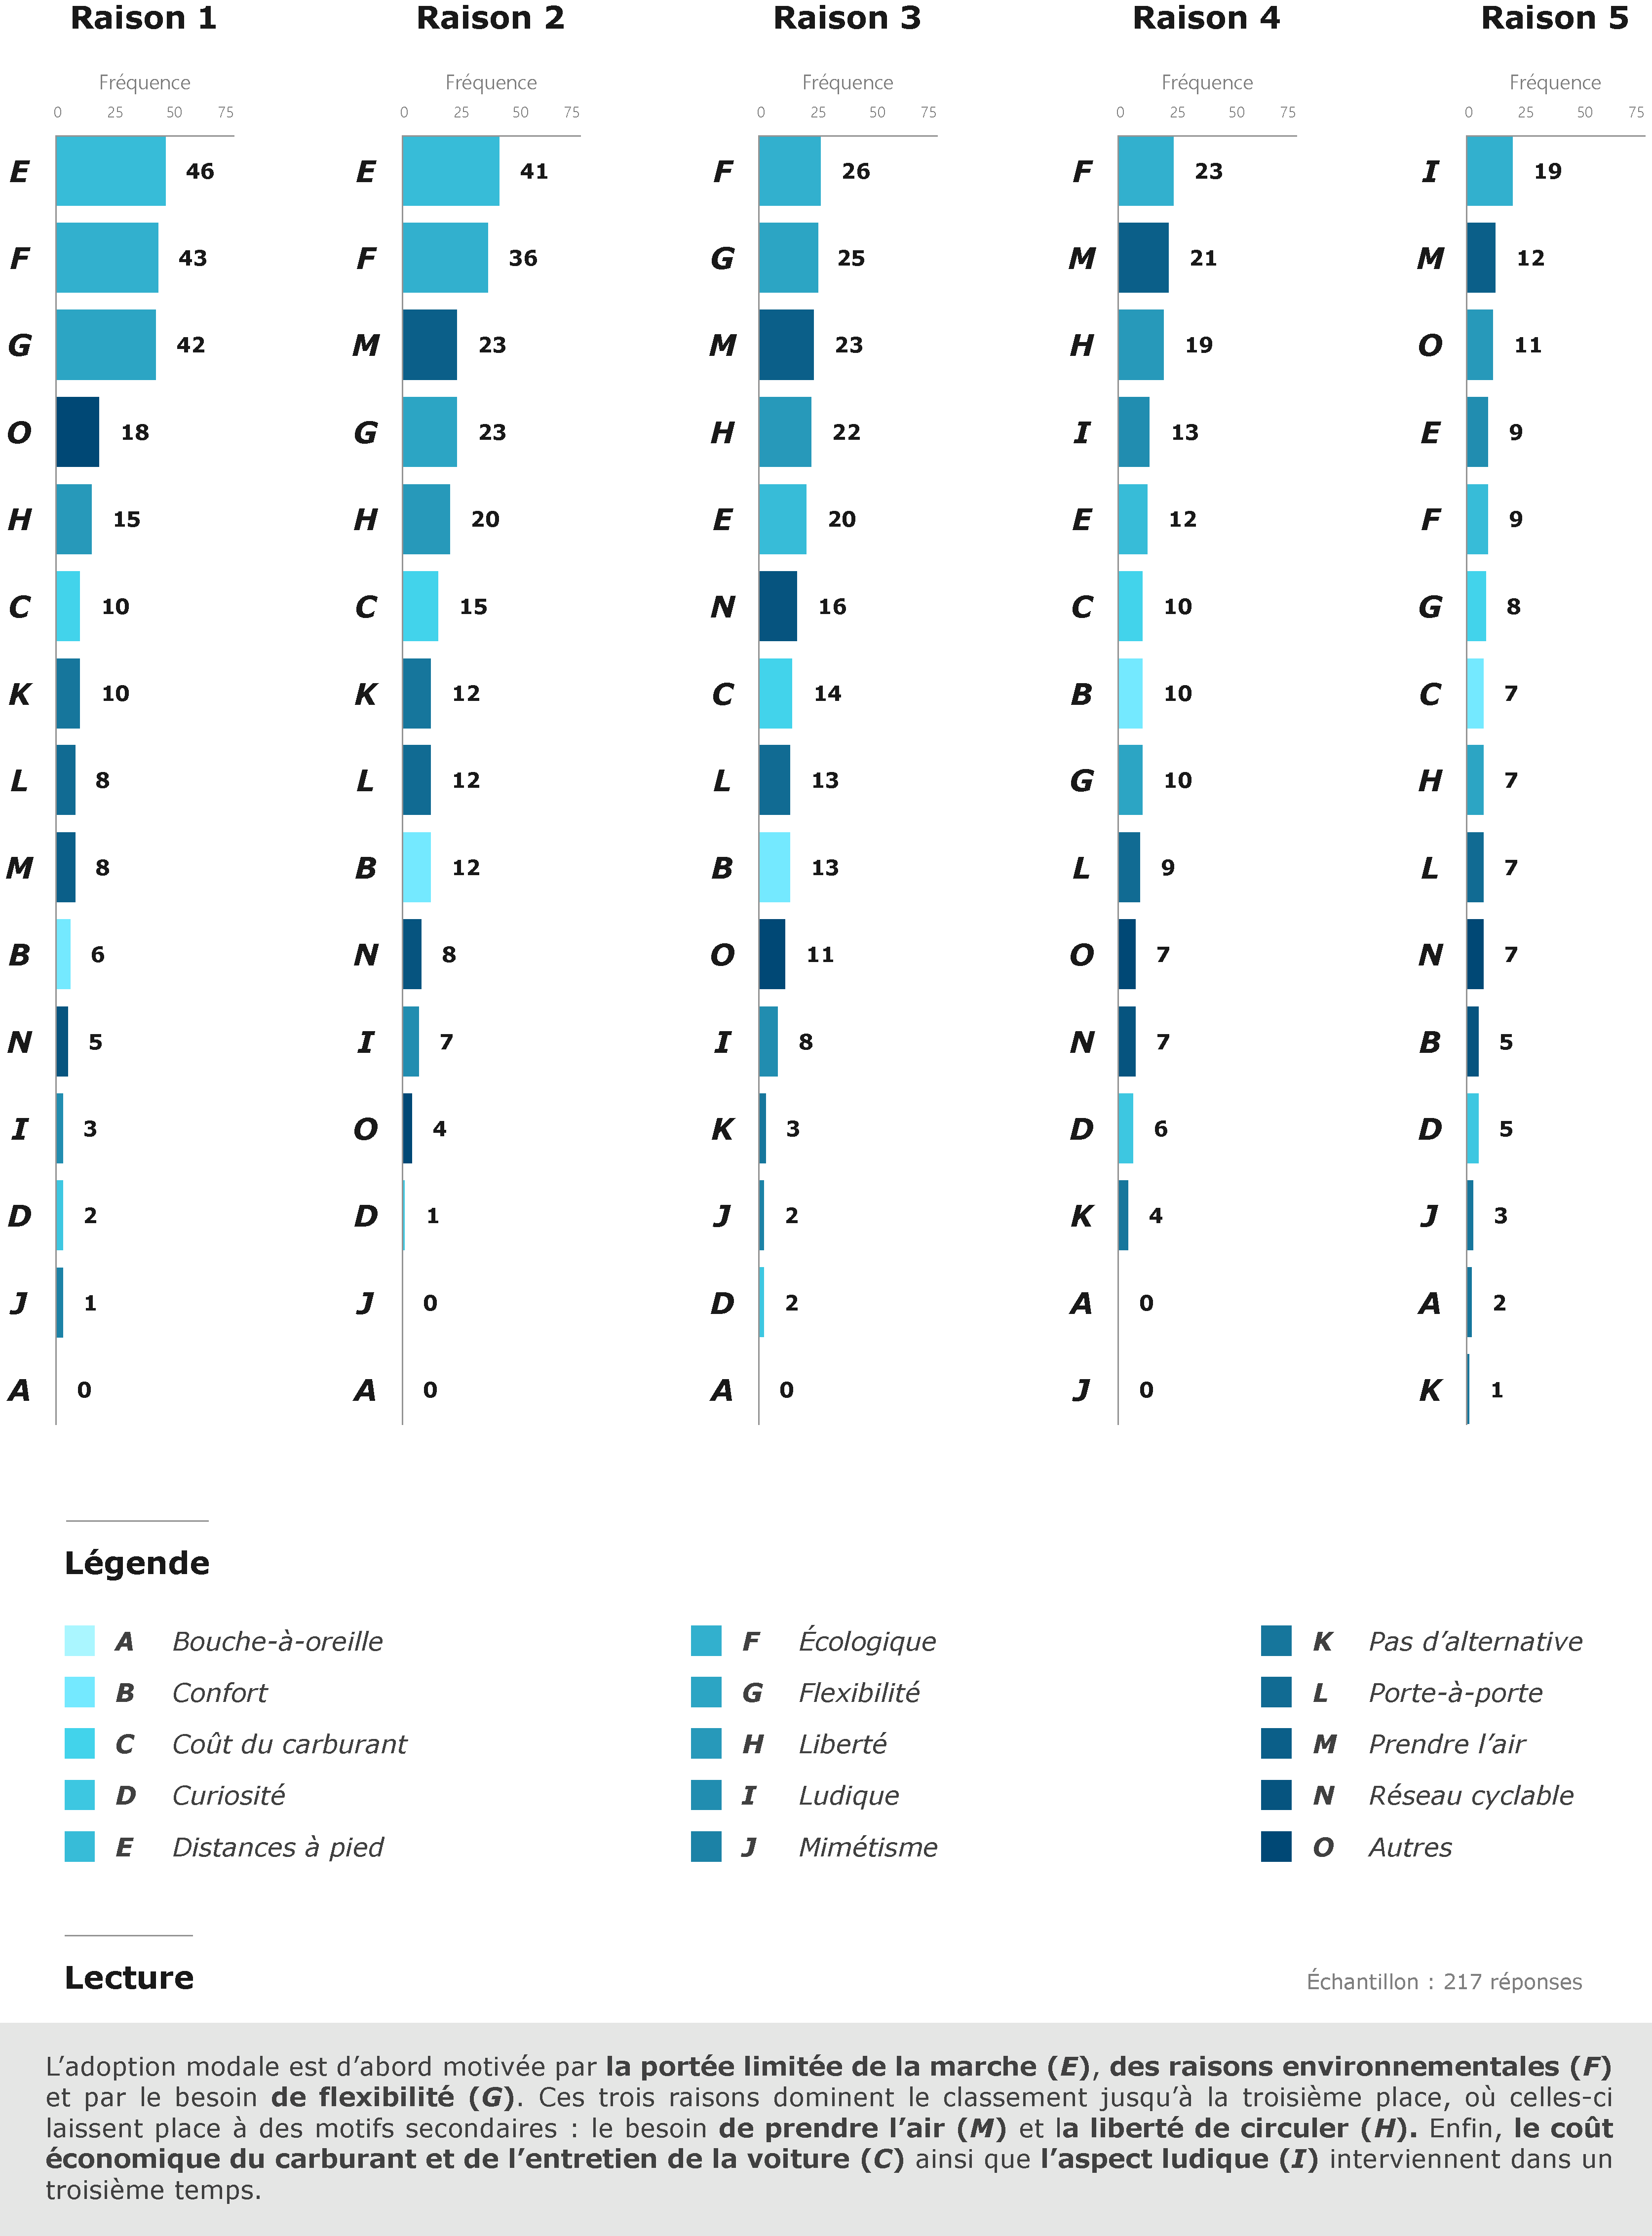
\includegraphics[width=1\columnwidth]{src/Figures/Chap-4/FR_Raisons_adoption.pdf}}
        \vspace{5pt}
        \begin{flushright}\scriptsize{
        Auteur~: \textcolor{blue}{Dylan Moinse (2024)}
        }\end{flushright}
    \end{figure}

    % Approche raisons adoption - points
Afin de considérer la hiérarchie des motifs invoqués par les participant·e·s pour expliquer leur choix modal, de la raison principale à la cinquième raison, nous avons mis en place un système de pondération des critères catégorisés. Cette approche attribue des points de manière dégressive en fonction du rang de chaque raison\footnote{
    Nous nous sommes servis de la méthode Borda (\textsl{Borda count method} en vue d'attribuer des points en fonction des préférences exprimées par les votant·e·s, un système qui détient l'avantage de ne pas exclusivement représenter les premiers choix. La raison principale octroie cinq points à la raison classée, avec un système dégressif jusqu'à un point pour la cinquième raison. Les variables qui n'ont pas été sélectionnées ne reçoivent alors pas de point.
}. Cette technique permettant de dépasser le raisonnement par occurrence met à disposition une distribution différenciée des motifs de choix modal (voir le \hyperref[table-chap4:raisons-adoption-modale-points]{tableau~\ref{table-chap4:raisons-adoption-modale-points}}, page~\pageref{table-chap4:raisons-adoption-modale-points}).%%Rédigé%%

    % Raisons adoption globale - points
Effectivement, les trois motivations les plus fréquemment citées~–~la \Guillemets{sensibilité environnementale} (\(F\), 492 points), la \Guillemets{distance excessive à parcourir à pied} (\(E\), 487 points) et les gains de \Guillemets{flexibilité} (\(G\), 405 points) précédemment présentés~–~gardent leur place de premier plan. Toutefois, le caractère \Guillemets{ludique} (\(I\), 112 points) régresse, tandis que les motivations associées à la \Guillemets{liberté de circuler} (\(H\), 266 points) et à l'envie de \Guillemets{prendre l'air} (\(M\), 255 points) se maintiennent. Par contraste, certaines raisons moins souvent citées sont mieux classées, comme en témoignent les \Guillemets{coûts économiques de l'utilisation de la voiture} (\(C\), 179 points) et l'avantage du \Guillemets{porte-à-porte} (\(L\), 152 points).%%Rédigé%%

    % Tableau Raisons adoption par points
% Tableau Raisons adoption par points
%%Rédigé%%
    \begin{table}[h!]
    \centering
    \renewcommand{\arraystretch}{1.5}
    \resizebox{\columnwidth}{!}{
    \begin{tabular}{p{0.07\columnwidth}p{0.06\columnwidth}p{0.4\columnwidth}p{0.1\columnwidth}p{0.1\columnwidth}p{0.1\columnwidth}}
        %\hline
    \rule{0pt}{15pt} \small{\textcolor{blue}{\textbf{Rang}}} & \small{\textcolor{blue}{\textbf{ID}}} & \small{\textcolor{blue}{\textbf{Raisons classées}}} & \small{\textcolor{blue}{\textbf{Points}}} & \small{\textcolor{blue}{\textbf{Top~3}}} & \small{\textcolor{blue}{\textbf{Effectif}}}\\
        \hline
\small{1} & \small{\(F\)} & \small{Sensibilité environnementale} & \small{\textbf{492}} & \small{105} & \small{137}\\
\small{2} & \small{\(E\)} & \small{Distances trop longues à pied} & \small{\textbf{487}} & \small{107} & \small{128}\\
\small{3} & \small{\(G\)} & \small{Gains de flexibilité} & \small{\textbf{405}} & \small{90} & \small{108}\\
        \hdashline
\small{4} & \small{\(H\)} & \small{Sensation de liberté} & \small{\textbf{266}} & \small{57} & \small{83}\\
\small{5} & \small{\(M\)} & \small{Prendre l'air} & \small{\textbf{255}} & \small{54} & \small{87}\\
\small{6} & \small{\(C\)} & \small{Coûts économiques de l'automobile} & \small{\textbf{179}} & \small{39} & \small{56}\\
\small{7} & \small{\(O\)} & \small{Autres raisons déclarées} & \small{\textbf{164}} & \small{33} & \small{51}\\
\small{8} & \small{\(L\)} & \small{Itinéraire porte-à-porte} & \small{\textbf{152}} & \small{33} & \small{49}\\
\small{9} & \small{\(B\)} & \small{Confort du déplacement} & \small{\textbf{142}} & \small{31} & \small{46}\\
\small{10} & \small{\(N\)} & \small{Présence d'un réseau cyclable} & \small{\textbf{126}} & \small{29} & \small{43}\\
\small{11} & \small{\(K\)} & \small{Absence d'alternative} & \small{\textbf{116}} & \small{25} & \small{30}\\
\small{12} & \small{\(I\)} & \small{Ludique} & \small{\textbf{112}} & \small{18} & \small{50}\\
\small{13} & \small{\(D\)} & \small{Curiosité} & \small{\textbf{37}} & \small{5} & \small{16}\\
\small{14} & \small{\(J\)} & \small{Mimétisme} & \small{\textbf{14}} & \small{3} & \small{6}\\
\small{15} & \small{\(A\)} & \small{Bouche-à-oreille} & \small{\textbf{2}} & \small{0} & \small{2}\\
    \hdashline
\multicolumn{3}{l}{\small{\textbf{Moyenne générale}}} & \small{\textbf{197}} & \small{\textbf{59}} & \small{\textbf{-}}\\
        \hline
        \end{tabular}}
    \caption{Répartition par point des raisons de l'adoption intermodale de la mobilité individuelle légère.}
    \label{table-chap4:raisons-adoption-modale-points}
        \vspace{5pt}
        \begin{flushleft}\scriptsize{
        \textcolor{blue}{Note~:} la colonne \textsl{Points} fait référence au nombre de points attribué de manière dégressive à chaque raison, la première position du classement octroyant cinq points, contre un point pour la cinquième position. La colonne \textsl{Top~3} correspond au nombre de fois où l'option a été placée dans les trois premiers choix parmi les réponses apportées.
        \\
        \textcolor{blue}{Lecture~:} à partir des 217 réponses analysées, les résultats montrent que la sensibilité environnement la perception des distances trop longues à pied sont les deux principales raisons qui motivent l'adoption intermodale de la mobilité individuelle légère, suivies par les gains de flexibilité qui complètent le trio de tête des motivations exprimées.
        }\end{flushleft}
        \begin{flushright}\scriptsize{
        Auteur~: \textcolor{blue}{Dylan Moinse (2024)}
        }\end{flushright}
        \end{table}%%Rédigé%%

    % Raisons adoption par modes - points
De la même manière, nous avons choisi d'analyser en profondeur les similitudes et les disparités entre les différents modes de déplacement, en employant cette fois-ci le système de pondération (voir l'\hyperref[fig-chap4:raisons-adoption-modale-points-modes]{illustration~\ref{fig-chap4:raisons-adoption-modale-points-modes}}, page~\pageref{fig-chap4:raisons-adoption-modale-points-modes}). Nous remarquons une distinction claire entre, d'une part, l'adoption intermodale des modes à propulsion humaine, à l'exception du \acrshort{VLS}, essentiellement motivée par des considérations écologiques et par la liberté de mouvement, et d'autre part, les utilisateur·rice·s de l'électromobilité, qui privilégient la souplesse, face aux charges financières de la voiture. Il se dégage ainsi que la \Guillemets{sensibilité environnementale} (\(F\)) constitue 21~\% des points totaux pour le vélo classique et 23~\% pour la trottinette mécanique. Cette proportion décroît à 16~\% pour le vélo pliant, à 12~\% pour le \acrshort{VAE} et même à 10~\% et à 9~\% respectivement pour les services de mobilité et la \acrshort{TEP}. En effet, pour le véhicule électrique et pliant, la \Guillemets{flexibilité} (\(G\)) est davantage valorisée, représentant 19~\% des points, tout comme pour la trottinette mécanique et le vélo pliant qui enregistrent respectivement 18~\% et 17~\%. Les \Guillemets{coûts économiques de l'utilisation de la voiture} (\(C\)) sont un autre critère prépondérant qui s'élèvent 13~\% pour la \acrshort{TEP}. En revanche, la sensation de \Guillemets{liberté de circuler} (\(H\)) est bien plus mise en avant par les usager·ère·s ayant adopté le vélo de tous types, contrairement à la trottinette de tous types et à la mobilité partagée.%%Rédigé%%

    % Figure treemap raisons adoption modale par modes et par points
    \begin{figure}[h!]\vspace*{4pt}
        \caption{Carte arborescente par point des raisons de l'adoption intermodale selon le type de véhicule.}
        \label{fig-chap4:raisons-adoption-modale-points-modes}
        \centerline{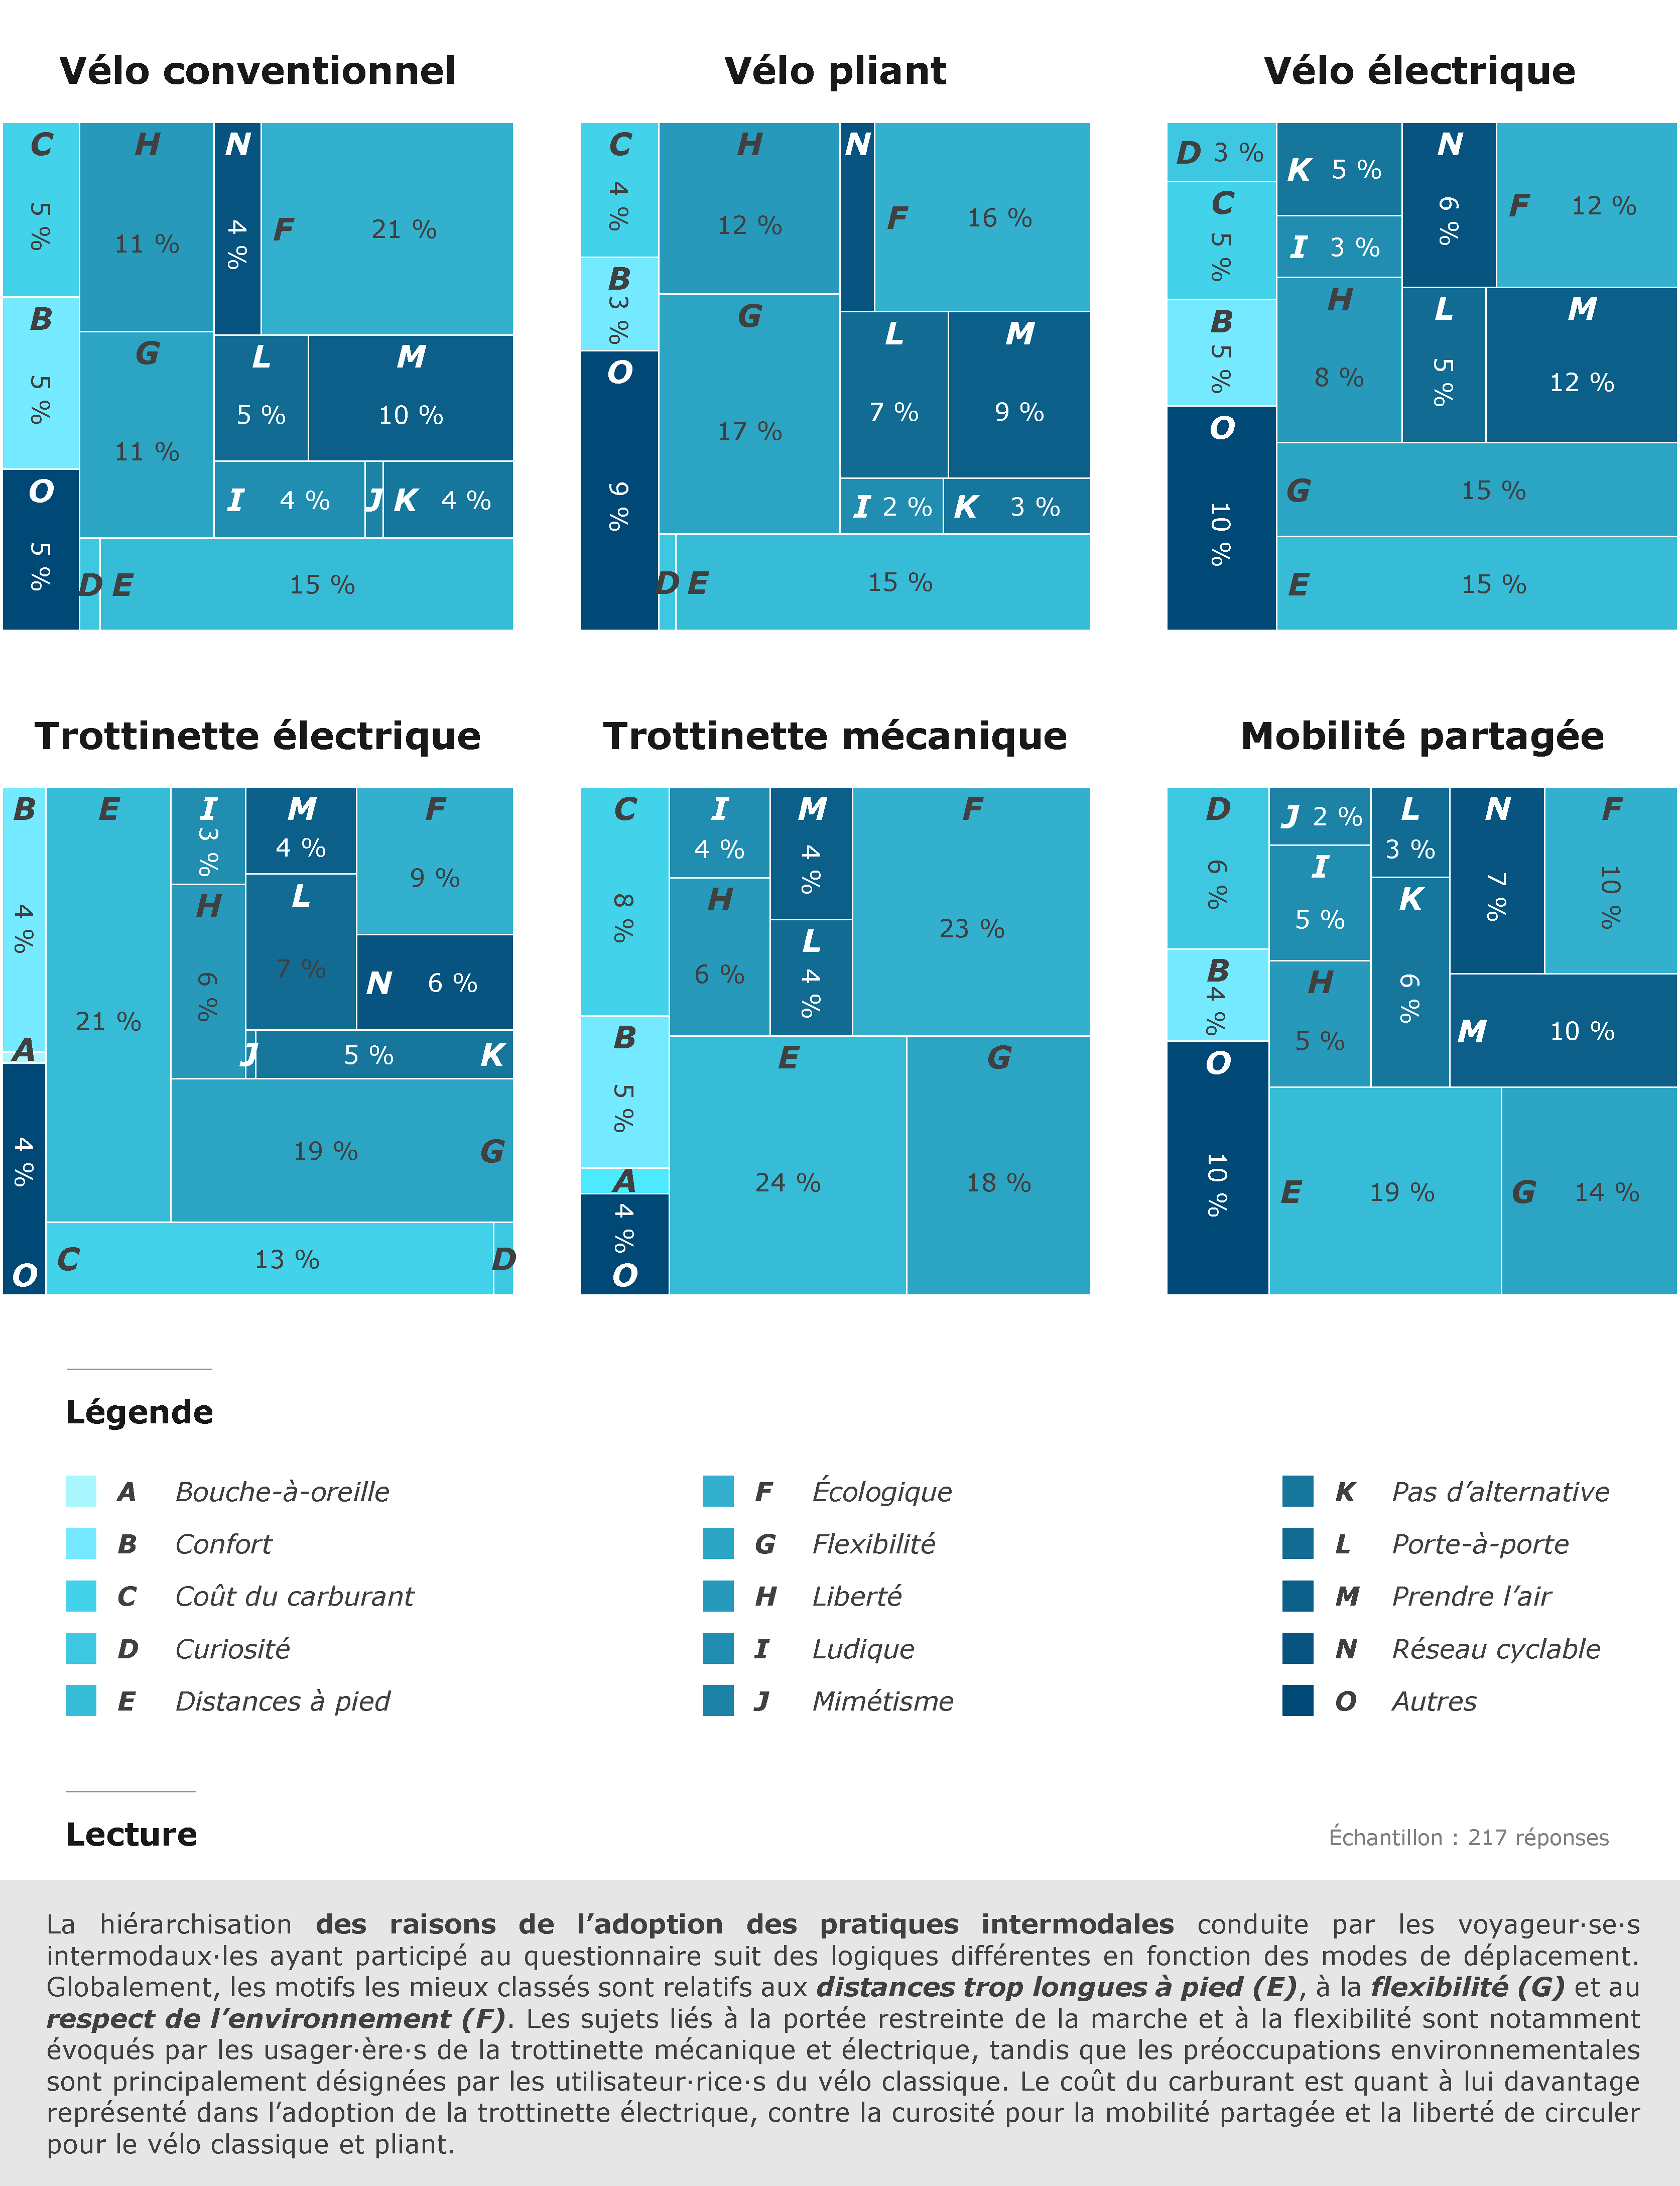
\includegraphics[width=1\columnwidth]{src/Figures/Chap-4/FR_Treemap_raisons_adoption.pdf}}
        \vspace{5pt}
        \begin{flushright}\scriptsize{
        Auteur~: \textcolor{blue}{Dylan Moinse (2024)}
        }\end{flushright}
    \end{figure}

    % Raisons autres - global
Un nombre important de classements réalisés a toutefois compris des réponses de type \Guillemets{autres}, enrichies de réponses libres textuelles. Parmi les 51 raisons supplémentaires évoquées et détaillées par les répondant·e·s, la quête de \Guillemets{gains de distance-temps} (17 réponses) émerge comme l'argument le plus fréquemment cité. Cette motivation est suivie par la recherche de \Guillemets{bienfaits pour la condition physique} (9 réponses), d'\Guillemets{économies réalisées sur l'abonnement de transport en commun urbain} (6 réponses) et d'une solution aux \Guillemets{problèmes de stationnement de congestion automobile} (6 réponses). D'autres réponses textuelles ont été regroupées autour de la \Guillemets{réduction du temps d'attente aux arrêts de bus} (5 réponses), d'une \Guillemets{plus grande flexibilité hors des heures de pointe} (3 réponses), d'un \Guillemets{substitut durant les périodes de grève} (3 réponses) et en réaction à des \Guillemets{mesures incitatives mises en place par l'employeur·se} (2 réponses).%%Rédigé%%

    % Raisons autres - hiérarchie
Sur le plan de la classification des motivations influençant le choix modal, les \Guillemets{gains de distance-temps} (72 points) restent prééminents, occupant fréquemment la première position, à l'instar des \Guillemets{problèmes de stationnement de congestion automobile} (24 points). Certaines raisons catégorisées sont quant à elles considérées comme secondaires, telles que les \Guillemets{bienfaits pour la condition physique} (21 points), la \Guillemets{réduction du temps d'attente aux arrêts de bus} (17 points) et la \Guillemets{plus grande flexibilité hors des heures de pointe} (10 points). En revanche, bien que les \Guillemets{économies réalisées sur l'abonnement de transport en commun urbain} (9 points) soient régulièrement mentionnées, elles sont souvent reléguées au rang de motivation mineure.%%Rédigé%%

    % Littérature raisons adoption
Plusieurs recherches ont été consacrées aux facteurs influençant l'adoption de la mobilité individuelle légère, en usage exclusif. Nos observations coïncident avec les tendances générales qui identifient les principaux motifs d'adoption de ces modes de déplacement~: la recherche de gain de temps et d'un sentiment de liberté de circulation, suivie par des motivations environnementales et économiques. \textcolor{blue}{\textcite[16-17]{pages_nouveaux_2021}}\index{Pages, Thibaud|pagebf}\index{Lammoglia, Adrien|pagebf}\index{Josselin, Didier|pagebf} se sont penché·e·s sur les éléments attractifs des \acrfull{NVEI} en France, incluant principalement le monoroue, le \acrshort{VAE} et la \acrshort{TEP}. Leurs résultats mettent en évidence, en premier choix, une envie de \Guillemets{changer de mode} (27~\%), de \Guillemets{gagner du temps} (18~\%), d'\Guillemets{être à l'extérieur} (17~\%), des \Guillemets{raisons écologiques} (16~\%), de \Guillemets{réaliser des économies} (13~\%) et de jouir d'une plus grande \Guillemets{flexibilité dans le choix de leurs itinéraires} (9~\%). Par ailleurs, une classification semblable issue de l'étude menée par la \textcolor{blue}{\textcite[15]{smart_mobility_lab_usages_2020}}\index{Smart Mobility Lab@\textsl{Smart Mobility Lab}|pagebf} indique que les utilisateur·rice·s d'un \acrfull{EDP} en monomodalité valorisent particulièrement l'\Guillemets{autonomie} et la \Guillemets{réduction du temps} de déplacement. Ces raisons sont suivies par des considérations \Guillemets{économiques} et \Guillemets{ludiques}, ainsi que par des aspects \Guillemets{écologiques} et \Guillemets{futuristes}, tandis que la place accordée aux activités physiques est marginale. Enfin, une enquête menée auprès des voyageur·se·s du chemin de fer en France appuie des motivations comparables qui animent leur choix modal~: la praticité, la rapidité, ainsi que les avantages écologiques et économiques des services de transport en commun \textcolor{blue}{\autocite[24]{toluna_francais_2023}}\index{Toluna@\textsl{Toluna}|pagebf}\index{Harris Interactive@\textsl{Harris Interactive}|pagebf}.%%Rédigé%%

    % Transition
La présente sous-section soutient le caractère émergent de l'intégration de la mobilité individuelle légère au réseau de transport en commun, stimulé notamment par l'introduction récente de certains véhicules sur le marché. Toutefois, il demeure incertain de savoir si cette évolution représente une réelle progression du système de mobilité alternative, plutôt qu'un simple remplacement des modes de déplacement traditionnels, typiquement le vélo, par les véhicules étudiés. Dans ce contexte, nous sommes amené·e·s à nous intéresser à l'effet de substitution modale induit par l'usage intermodal du vélo et de la micro-mobilité.%%Rédigé%%

    % 4.2.1.3.
    \needspace{1\baselineskip} % Réserve de l'espace
\subsubsection*{Un effet de substitution modale à double tranchant
    \label{chap4:substitution-modale-double-tranchant}
    }

    % Substitution modale - globale
À la problématique de l'effet de substitution modale de l'interaction entre la mobilité individuelle légère et le transport public, nous avons intégré une question spécifique sur la concurrence modale au sein du questionnaire destiné aux cyclo-voyageur·se·s. Nous leur avons posé la question suivante~: \Guillemets{Si vous n'aviez pas pu utiliser votre vélo ou votre engin de déplacement, quel autre moyen auriez-vous employé pour rejoindre votre gare de départ ou votre lieu de destination, depuis la gare d'arrivée~?} (voir l'\hyperref[annexes:structure-questionnaire-usagers]{annexe~\ref{annexes:structure-questionnaire-usagers}}, page~\pageref{annexes:structure-questionnaire-usagers}). L'analyse des réponses apportées dévoile que la majorité des participant·e·s serait capable de s'adapter en remplaçant leur véhicule par d'autres modes de transfert. Précisément, en cas d'indisponibilité de leur vélo ou de leur micro-mobilité pour le pré-acheminement ou le post-acheminement, 78~\% des sondé·e·s opteraient pour un autre mode de déplacement en rabattement et, ou bien, en diffusion (169 réponses), tandis que 13~\% des répondant·e·s envisageraient de modifier complètement leur choix modal pour l'ensemble du déplacement intermodal (29 réponses). Enfin, 9~\% des enquêtée·e·s renonceraient au déplacement (19 réponses).%%Rédigé%%

    % Substitution modale - rabattement et diffusion
Les données collectées illustrent la tendance marquée des répondant·e·s à favoriser certains modes de déplacement, en l'absence de leur premier choix de transfert vers et depuis les nœuds de transport en commun. En particulier, les systèmes de transport en commun urbain et la marche combinée émergent comme des alternatives privilégiées, avec des variations notables entre les étapes de leur déplacement intermodal de référence. Pour le rabattement comme pour la diffusion, 43~\% des participant·e·s se reporteraient vers un mode de transport en commun urbain pour accéder à la gare d'origine (72 réponses), contre 38~\% en sortant de la gare de destination (64 réponses). La marche combinée est privilégiée par 37~\% des sondé·e·s en rabattement (63 réponses), contre 54~\% en diffusion (91 réponses). Seul·e·s 8~\% des voyageur·se·s se tourneraient vers l'utilisation de la voiture en pré-acheminement (13 réponses), aussi bien en tant que conducteur·rice que passager·ère, alors que ce report modal chute respectivement à 1~\% et à 6~\% en post-acheminement (12 réponses). La mobilité partagée est quant à elle choisie par 3~\% des personnes enquêtées, exclusivement en rabattement (5 réponses). Enfin, l'option du taxi et de la \acrfull{VTC} représente 2~\%, pour les \Guillemets{premiers kilomètres}, et 1~\%, pour les \Guillemets{derniers kilomètres} des réponses déclarées (5 réponses).%%Rédigé%%

    % Substitution - totale
Parmi celleux renonçant complètement au mode collectif au cours du déplacement projeté (13~\%, 29 réponses), les données recueillies montrent une inclination importante des répondant·e·s à opter pour la voiture individuelle, à la différence des modes de transfert précédemment mentionnés. 76~\% d'entre elleux privilégieraient l'usage exclusif de la voiture en tant que conducteur·rice (22 réponses). Le covoiturage, représentant 14~\% des choix (4 réponses), et l'usage de la voiture en tant que passager·ère, à hauteur de 7~\% (2 réponses), demeurent marginaux, tout comme le scooter qui n'attire que 3~\% des répondant·e·s (1 réponse).%%Rédigé%%

    % Synthèse
Dans l'ensemble des scénarios envisagés, le report modal se fait avant tout vers la marche et les transports en commun urbains, avec respectivement 42~\% et 37~\% (154 et 136 réponses) des préférences exprimées. La conduite automobile suit avec 10~\% (37 réponses), tandis que le rôle de passager·ère, appelé également \textsl{kiss-and-ride}, est choisi par 7~\% des participant·e·s (25 réponses). Peut-on pour autant en déduire que l'usage intermodal de la mobilité individuelle légère tend principalement à remplacer la marche combinée~? À cet égard, l'analyse statistique indique que le choix de la marche est souvent associé, aux extrémités du déplacement intermodal, à l'usage de l'automobile~: les voyageur·se·s qui ont déclaré sortir de la gare à pied sont régulièrement des automobilistes en rabattement. Ce phénomène révèle une complexité sous-jacente dans la configuration des déplacements intermodaux, où la marche combinée est le mode de déplacement le plus vulnérable à la substitution modale. Toutefois, simultanément, l'utilisation de la voiture est également remplacée par les pratiques intermodales étudiées. Cette dualité suggère que, bien que la marche puisse être fréquemment remplacée, elle reste étroitement liée, dans le cadre des comportements de mobilité spécifiques aux cyclo-voyageur·se·s, à l'usage automobile.%%Rédigé%%

    % Figure Distances substitution marche
    \begin{figure}[h!]\vspace*{4pt}
        \caption{Estimation du report modal depuis la marche combinée au regard des distances spatiales parcourues en transfert, à vélo et en micro-mobilité.}
        \label{fig-chap4:distances-substitution-modale}
        \centerline{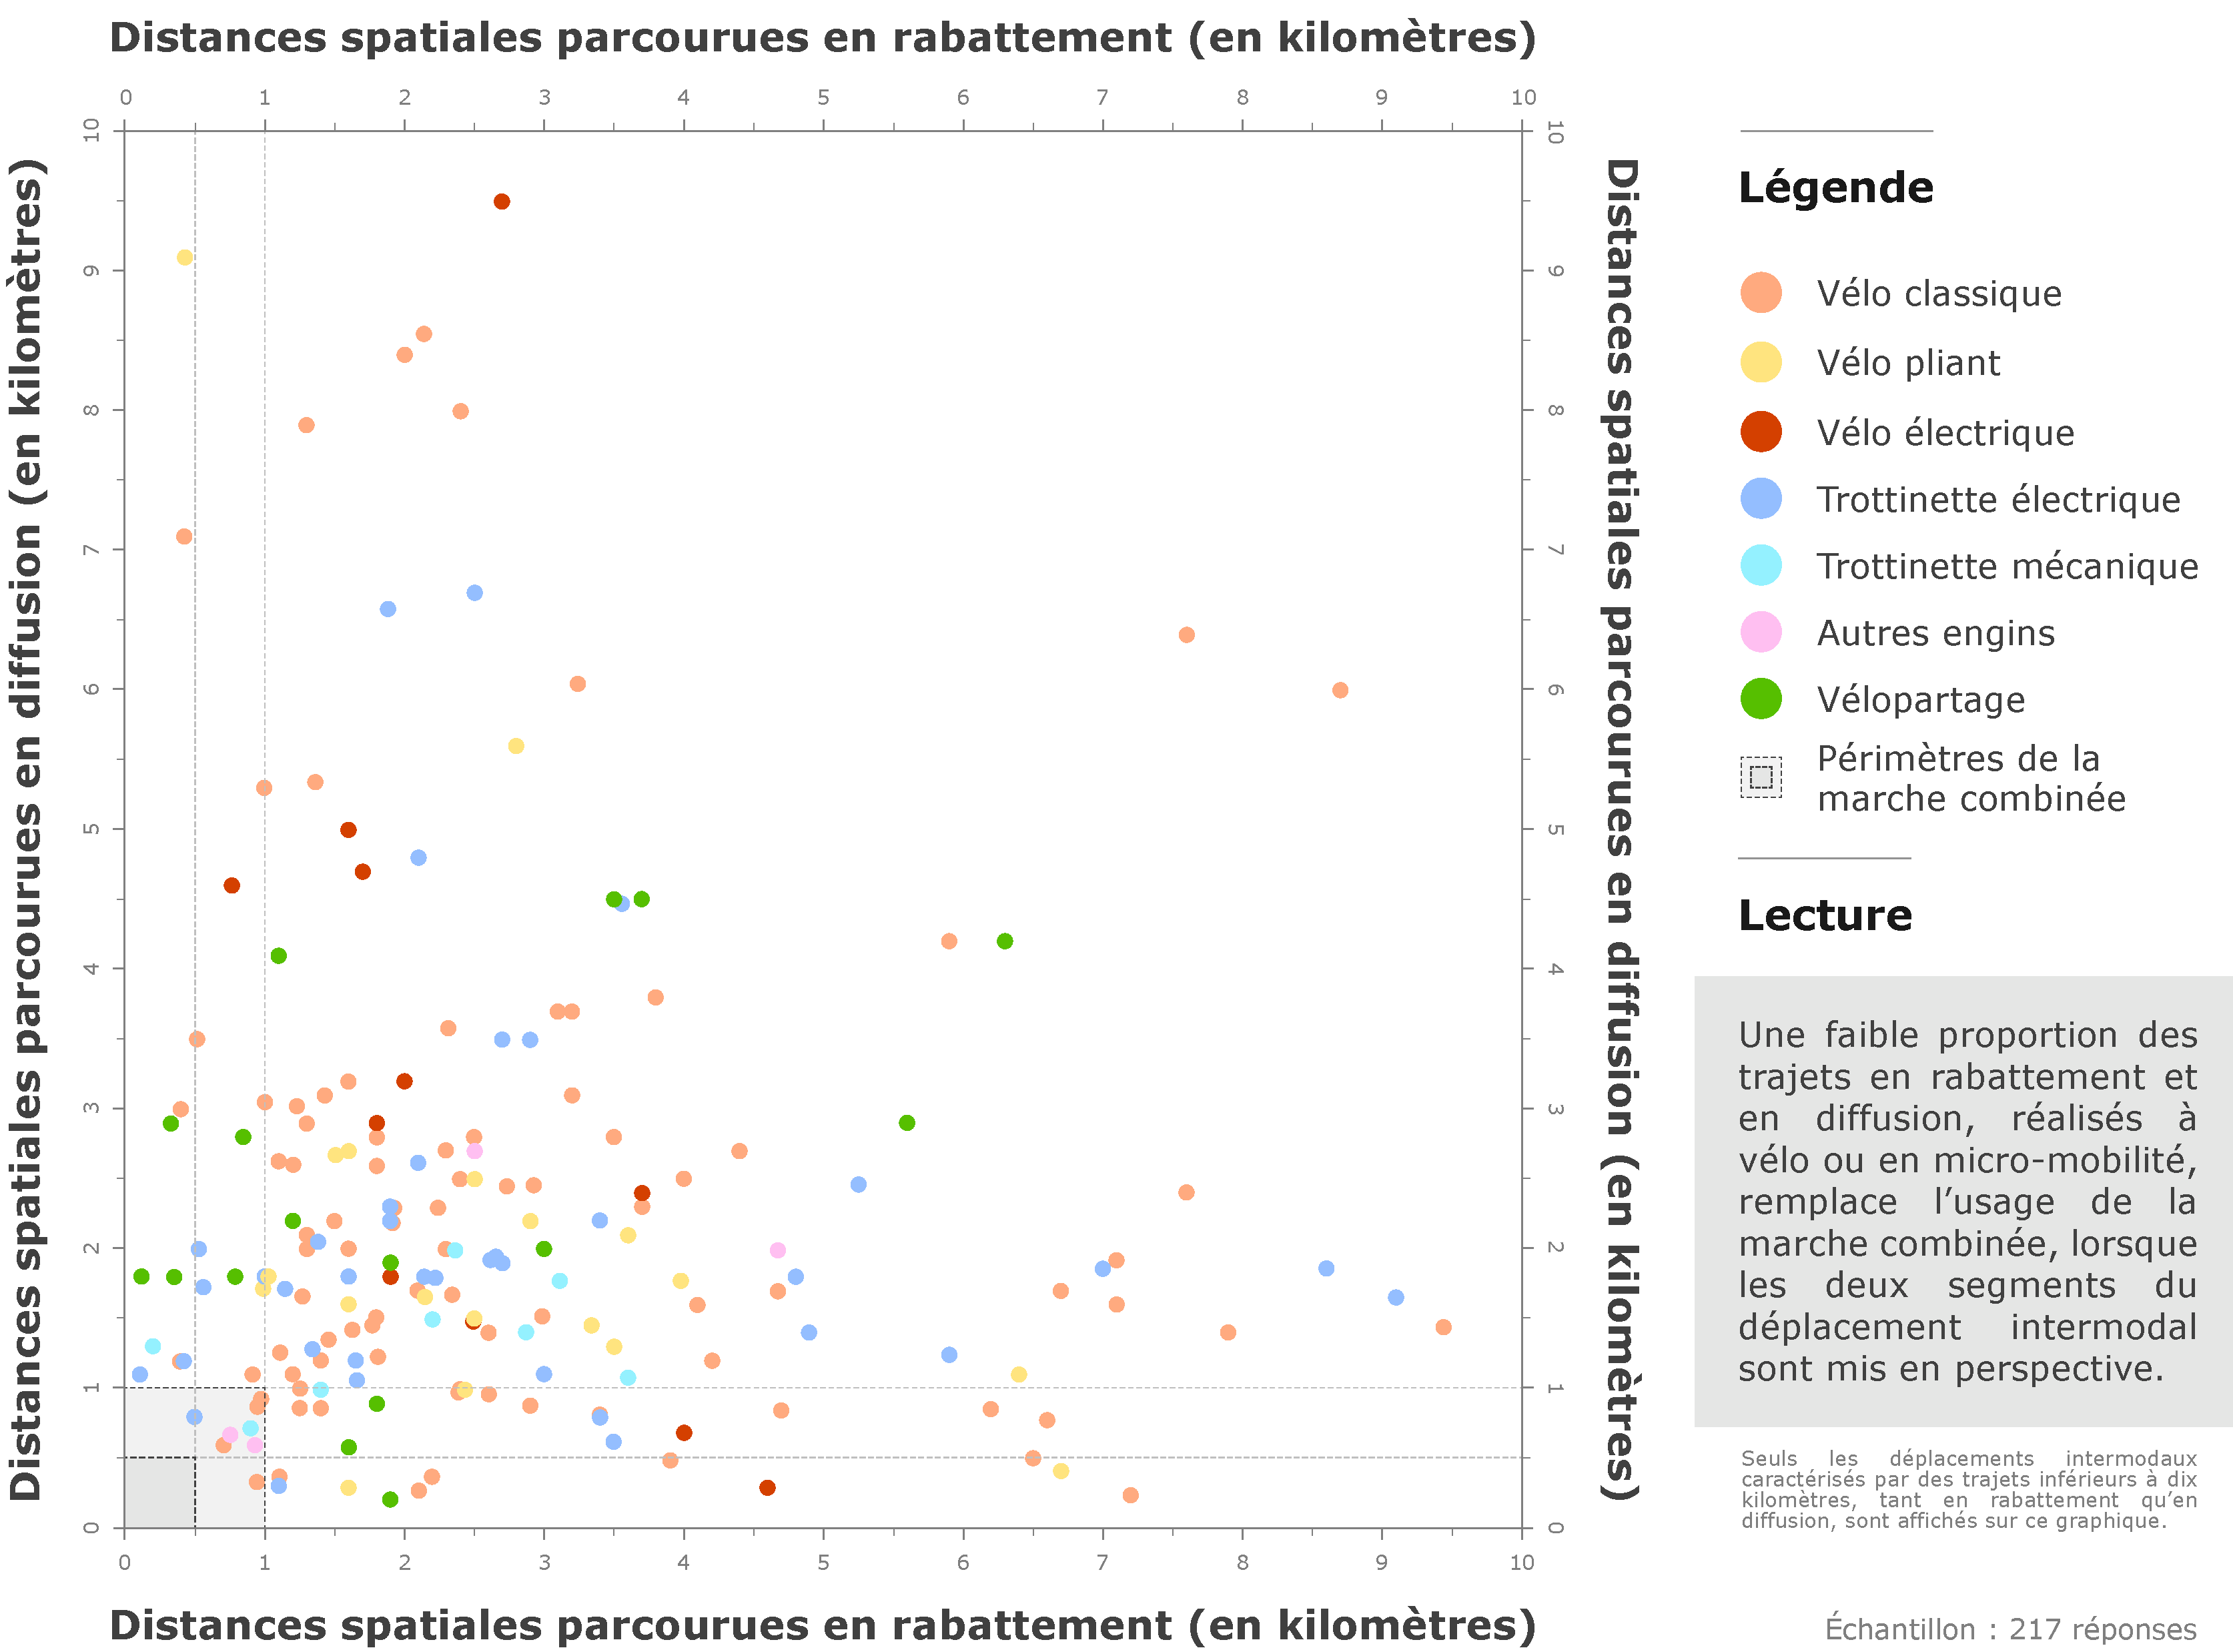
\includegraphics[width=1\columnwidth]{src/Figures/Chap-4/FR_Distances_substitution_modale.pdf}}
        \vspace{5pt}
        \begin{flushright}\scriptsize{
        Auteur~: \textcolor{blue}{Dylan Moinse (2023)}
        }\end{flushright}
    \end{figure}

    % Distance rabattement et diffusion
L'argument soutenant que la substitution de la marche combinée témoigne d'une répercussion à double tranchant sur les choix modaux peut être corroboré par une analyse détaillée des distances spatiales parcourues par les voyageur·se·s intermodaux·les. L'intention est alors de dépasser la nature déclarée des réponses pour établir dans quelle mesure certains trajets, tant en rabattement qu'en diffusion, auraient pu être effectués à pied compte tenu de la distance parcourue. Sur l'ensemble des 358 trajets effectués à vélo ou en micro-mobilité, il apparaît que seulement 12 itinéraires présentent une longueur inférieure à 0,50 kilomètre et 38 restent en dessous de 1 kilomètre. Cela représente 11~\% de segments susceptibles d'être réalisés à pied, en partant d'une portée élargie de la marche combinée, de l'ordre de 1 kilomètre \textcolor{blue}{\autocite[34]{canepa_bursting_2007}}\index{Canepa, Brian|pagebf}. Parmi ces 38 trajets de moins de 1 kilomètre, 18 ont été effectués à vélo classique, 8 en \acrshort{TEP}, 5 en vélo pliant, 4 en trottinette mécanique, 2 en \textsl{skateboard} et 1 en \acrshort{VAE}. En adoptant une perspective relative aux parts modales observées, la trottinette mécanique comme le \textsl{skateboard} sont les formes de micro-mobilité qui tendent à remplacer davantage la marche combinée.%%Rédigé%%

    % Discussion distance rabattement et diffusion
Cependant, une analyse simultanée des distances spatiales parcourues à la fois en pré-acheminement et en post-acheminement démontre qu'aucun des trajets n'affiche une distance inférieure à 0,50 kilomètre pour chacun des segments du déplacement intermodal. En outre, seuls 8 trajets affichent des trajets de moins de 1 kilomètre de part et d'autre du déplacement (voir l'\hyperref[fig-chap4:distances-substitution-modale]{illustration~\ref{fig-chap4:distances-substitution-modale}}, page~\pageref{fig-chap4:distances-substitution-modale}). Ce résultat suggère que seulement 2~\% des trajets effectués à vélo ou en micro-mobilité, dans le cadre d'un chaînage modal, se substituent effectivement à la marche combinée. Les réponses basées sur un report modal depuis le mode pédestre soulèvent alors des questions, car elles indiquent que, bien que la marche ait été envisageable, elle n'aurait pas été réalisable sur l'intégralité des \Guillemets{premiers et derniers kilomètres}. À ce titre, il semble exister un décalage notable entre l'effet de substitution modale de la marche déduit de l'analyse des itinéraires et estimé par les réponses déclarées. Cet écart pourrait alors s'expliquer par le choix des usager·ère·s d'opter pour des trajets plus étendus vers, ou depuis des nœuds de transport en commun qui ne sont pas nécessairement les plus proches de leurs points de départ ou de destination, grâce à l'utilisation de la mobilité individuelle légère, alors que des alternatives pédestres vers des arrêts plus rapprochés auraient pu être possibles. Cette hypothèse sera notamment approfondie dans la \hyperref[chap5:discussion-detours-pauses-optimisation]{section consacrée à l'étude des détours~\ref{chap5:discussion-detours-pauses-optimisation}} (page~\pageref{chap5:discussion-detours-pauses-optimisation}), dans le \hyperref[chap5:titre]{chapitre~5~\ref{chap5:titre}} (page~\pageref{chap5:titre}).%%Rédigé%%

    % Substitution modale réelle
Il apparaît clairement que l'effet de substitution modale en faveur de la mobilité individuelle légère couplée au transport public se fait principalement aux dépens des réseaux de transport en commun urbain, en particulier des services de bus. Cette transition modale peut être attribuée à une certaine méfiance envers l'offre de bus urbains, jugée insuffisamment compétitive face à la demande croissante de flexibilité \textcolor{blue}{\autocite[19-24]{bauman_liquid_2000}}\index{Bauman, Zygmunt|pagebf}, mieux satisfaite par la mobilité individuelle légère. La participante du parcours commenté, désignée sous le nom de \(PCTE_{1}\), illustre cette situation en relatant son choix de ne pas emprunter le bus une fois arrivée en gare de Maubeuge, en raison du temps d'attente perçu comme excessif. Elle indique qu'elle se serait intégralement déplacée en voiture si sa \acrshort{TEP} n'était pas disponible, soulignant la perte de compétitivité du train comparé à l'automobile dans ce contexte~: \Guillemets{\textsl{L'avantage aussi, c'est de pouvoir direct sortir de la gare et d'arriver à destination, sans devoir attendre le bus. Je pense que le temps d'attente du bus m'aurait fait arrêter de prendre le train.} [\dots] \textsl{car je me retrouve à devoir prendre le bus à Maubeuge. Et donc devoir prendre un abonnement, attendre le bus\dots~Et le soir, j'ai pas forcément confiance d'attendre\dots}} [12:18 et 17:14, \(PCTE^{TC}_{1}\)]. Par ailleurs, cette étude montre également que les pratiques intermodales peuvent efficacement remplacer l'utilisation de l'automobile, en renforçant la compétitivité du transport public lorsque ni la marche ni le bus ne fournissent une alternative suffisamment agile. L'usager \(PCTE_{2}\) nous explique que, bien que capable de marcher jusqu'à l'arrêt de métro République~-~Beaux-Arts, ce dernier préfère se déplacer en \acrshort{TEP} du fait que son véhicule est indispensable pour le segment en diffusion, où la marche serait trop chronophage. Il reconnaît alors que sans sa trottinette, il recourrait à l'automobile pour l'intégralité du déplacement [08:20, \(PCTE^{TC}_{E}\)].%%Rédigé%%

    % Changement de mobilité 1
À partir de l'analyse de la question relative aux habitudes de mobilité des répondant·e·s au questionnaire~: \Guillemets{À quelle fréquence utilisez-vous ces différents modes de déplacement~?}, croisée avec la question suivante~: \Guillemets{Utilisez-vous davantage ou moins fréquemment ces différents modes de déplacement, depuis que vous avez adopté ces combinaisons modales~?} (voir l'\hyperref[annexes:structure-questionnaire-usagers]{annexe~\ref{annexes:structure-questionnaire-usagers}}, page~\pageref{annexes:structure-questionnaire-usagers}), nous avons été en mesure de déterminer les effets de ces pratiques intermodales sur les systèmes de mobilité concurrents, à l'échelle individuelle. À cet effet, chaque voyageur·se ayant pour habitude d'utiliser l'un des modes de déplacement concernés était automatiquement redirigé vers la question suivante consistant à déclarer si leur fréquence d'utilisation avait évolué, allant d'un usage \Guillemets{bien moins fréquent}, \Guillemets{moins fréquent}, \Guillemets{stable}, \Guillemets{plus fréquent} à \Guillemets{bien plus fréquent}.

    % Changement de mobilité 2
L'enquête a révélé une tendance marquée vers la réduction de l'utilisation du taxi, du \acrshort{VTC} et de l'automobile, aussi bien en tant que conducteur·rice que passager·ère, depuis le recours à des stratégies intermodales (voir l'\hyperref[fig-chap4:impacts-adoption-autres-modes]{illustration~\ref{fig-chap4:impacts-adoption-autres-modes}}, page~\pageref{fig-chap4:impacts-adoption-autres-modes}). Le transport automobile de passager·ère·s a alors subi une baisse de l'utilisation de ces services, pour 88~\% des retours exprimés (50 sur 57 réponses). Plus précisément, 75~\% ont signalé une réduction significative (43 sur 57 réponses). En parallèle, l'automobile, que ce soit en tant que conducteur·rice ou passager·ère, tend à être moins plébiscitée. Pour les conducteur·rice·s, 68~\% ont diminué leur fréquence d'utilisation (102 sur 151 réponses), avec 38~\% mentionnant une réduction conséquente (57 sur 151 réponses). Quant aux passager·ère·s, 51~\% ont rapporté une diminution (76 sur 150 réponses), dont 28~\% de manière prononcée (42 sur 150 réponses). Inversement, l'usage exclusif de la mobilité individuelle légère a augmenté pour près de la moitié des sondé·e·s (48~\%, 96 sur 201 réponses), incluant 27~\% qui l'utilisent désormais \Guillemets{bien plus fréquemment} (54 sur 201 réponses). Les transports en commun urbains présentent un tableau plus nuancé~: bien que 28~\% des usager·ère·s aient réduit leur utilisation (56 sur 203 réponses), une proportion presque équivalente l'a augmentée (29~\%, 58 sur 203 réponses). La fréquence de la marche reste globalement inchangée pour une majorité de répondant·e·s (58~\%, 118 sur 209 réponses), tandis que 30~\% se déplacent moins fréquemment à pied (63 sur 209 réponses), dont 22~\% de manière modérée (45 sur 209 réponses).%%Rédigé%%

    % Figure Impacts sur les systèmes de mobilité
    \begin{figure}[h!]\vspace*{4pt}
        \caption{Impacts des pratiques intermodales sur les habitudes de mobilité des usager·ère·s.}
        \label{fig-chap4:impacts-adoption-autres-modes}
        \centerline{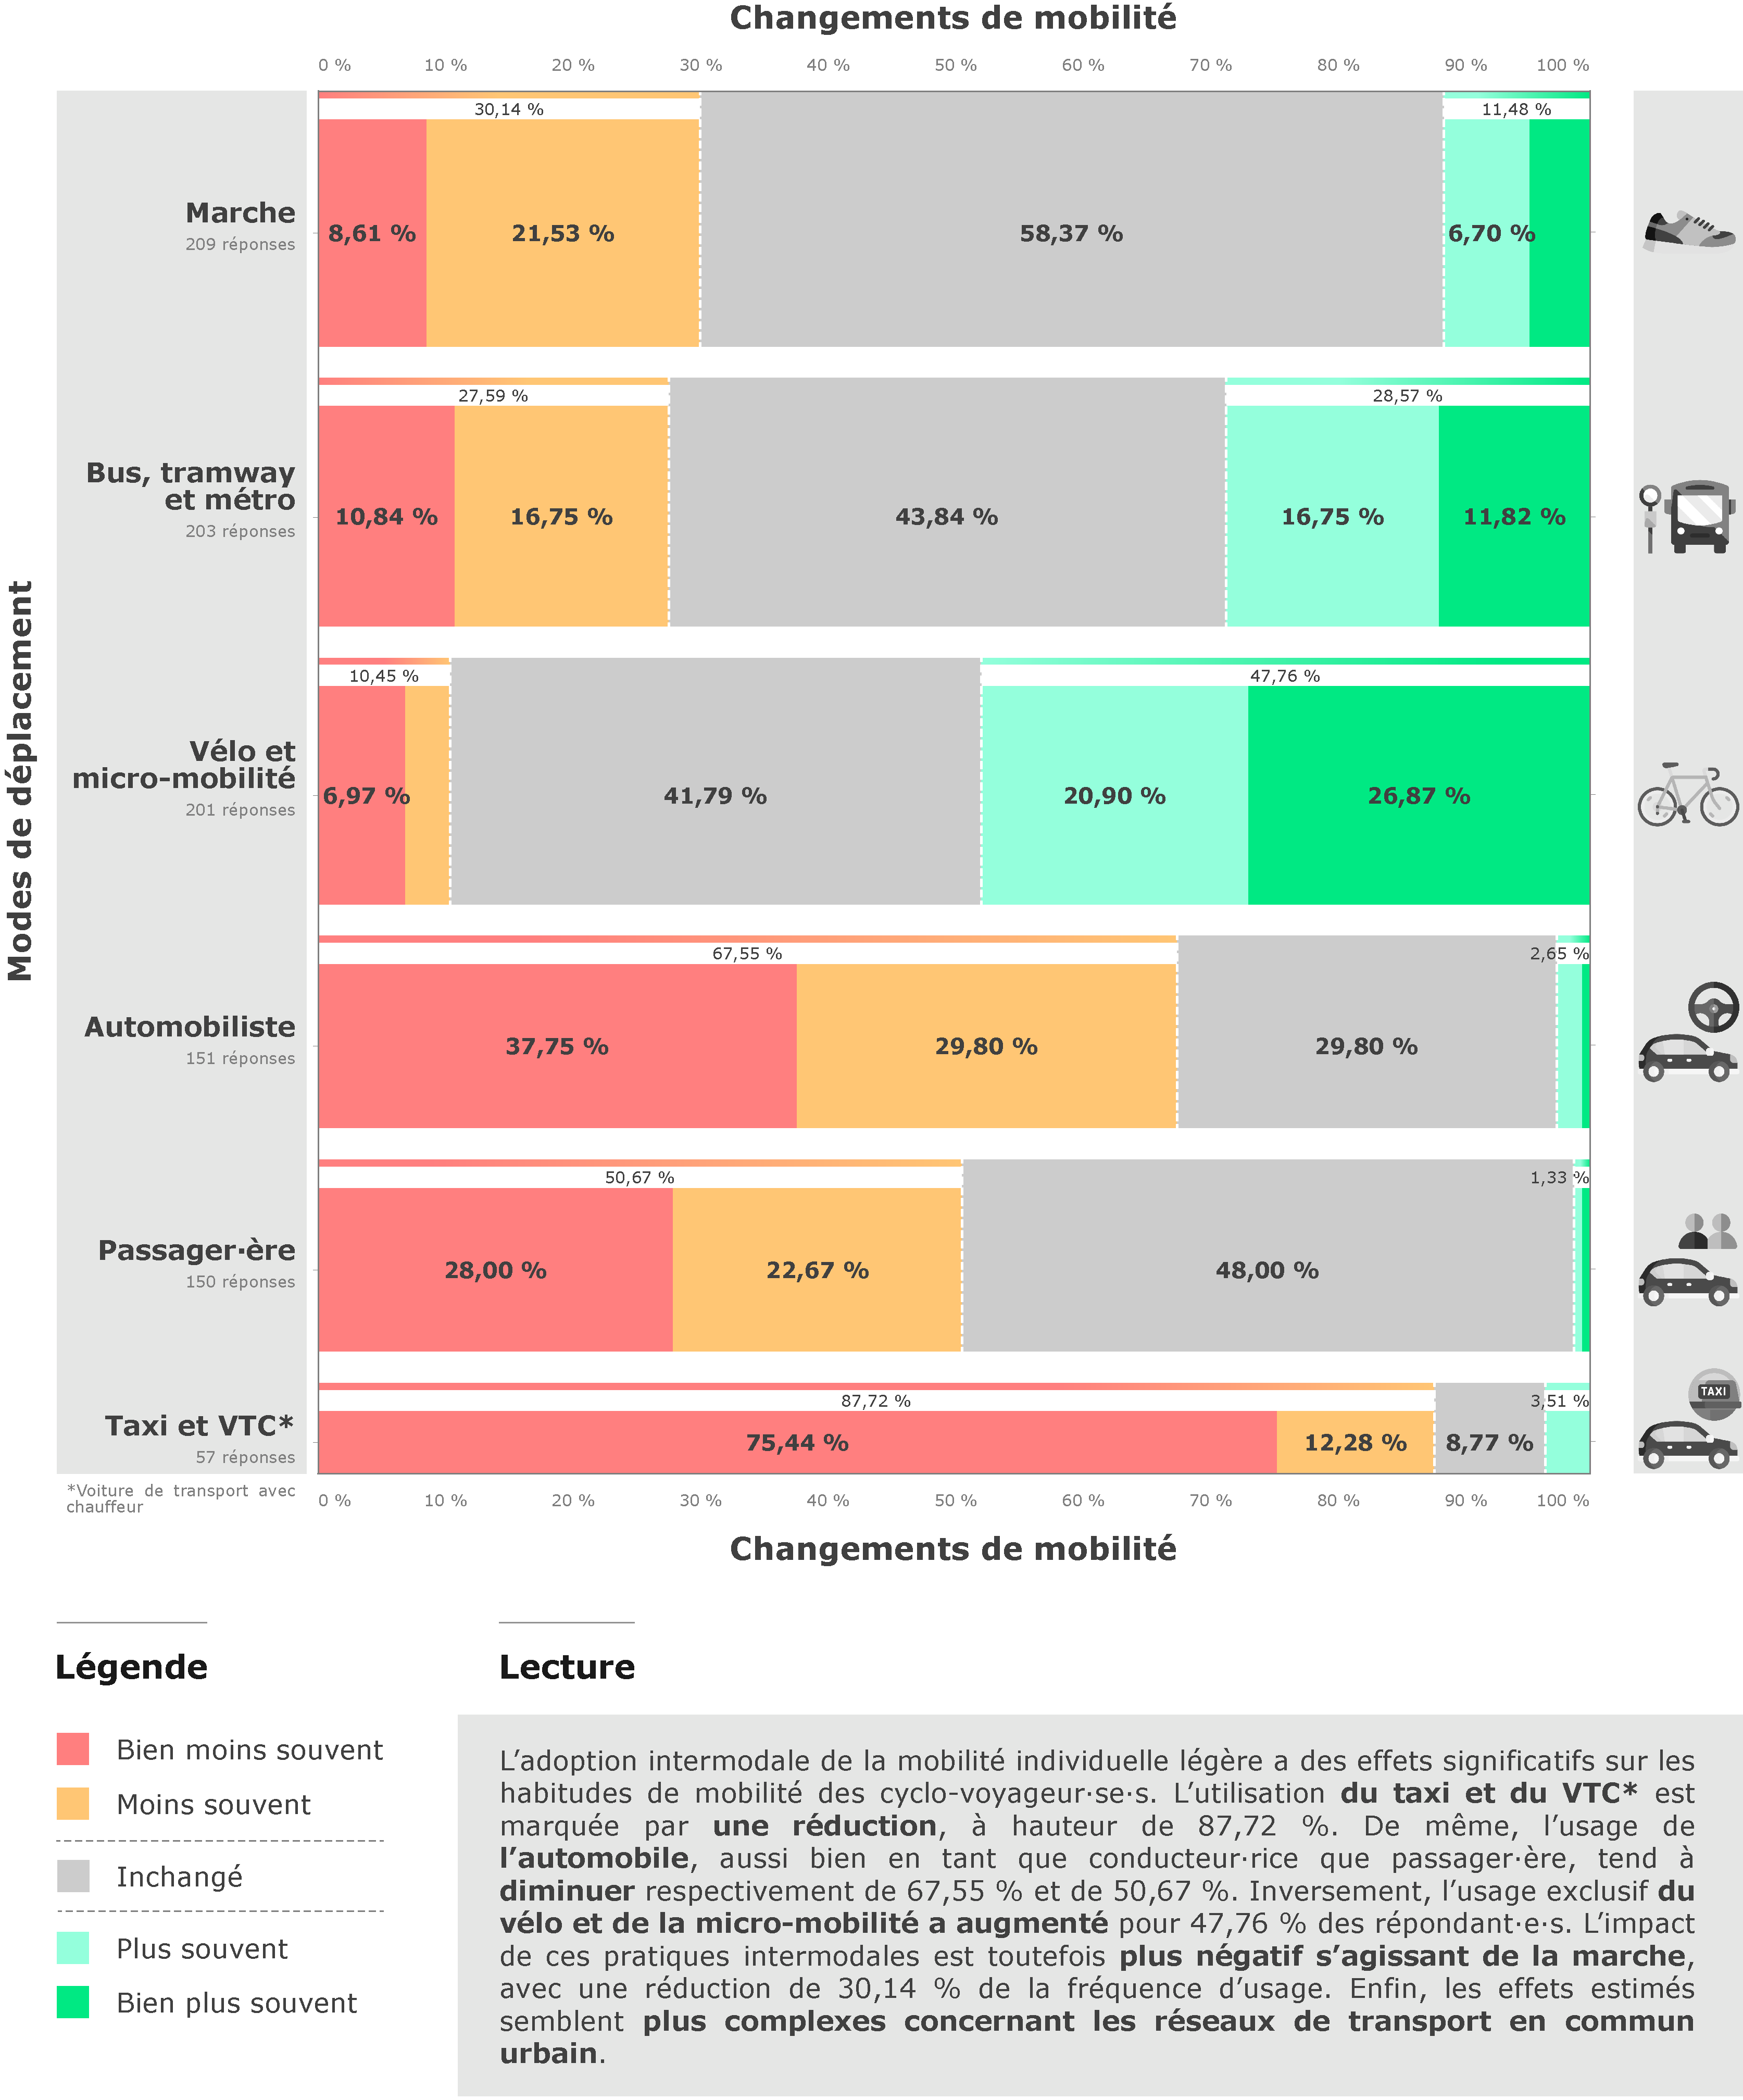
\includegraphics[width=1\columnwidth]{src/Figures/Chap-4/FR_Substitution_modale.pdf}}
        \vspace{5pt}
        \begin{flushright}\scriptsize{
        Auteur~: \textcolor{blue}{Dylan Moinse (2023)}
        }\end{flushright}
    \end{figure}

    % Littérature changement de mobilité - automobile
Les recherches académiques attestent partiellement l'hypothèse selon laquelle l'intégration de la mobilité individuelle légère aux systèmes de transport en commun contribue à une contraction conséquente de l'usage automobile. En France, il a été observé que 26~\% des usager·ère·s monomodaux·ales des \acrshort{NVEI} ont migré de l'automobile vers ces modes de déplacement alternatifs \textcolor{blue}{\autocite[14]{pages_nouveaux_2021}}\index{Pages, Thibaud|pagebf}\index{Lammoglia, Adrien|pagebf}\index{Josselin, Didier|pagebf}. Ces chercheurs ont également souligné que l'automobile, comme la moto et le scooter, ont subi un déclin de leur usage, rapporté pour 70~\% des utilisateur·rice·s des \acrshort{NVEI} \textcolor{blue}{\autocite[13]{pages_nouveaux_2021}}\index{Pages, Thibaud|pagebf}\index{Lammoglia, Adrien|pagebf}\index{Josselin, Didier|pagebf}. Pour ce qui est de l'usage intermodal du \acrshort{VLS}, le transfert modal depuis l'automobile à Montréal est estimé à 25~\%, dont une transition de 40~\% observée chez les résident·e·s des zones périurbaines \textcolor{blue}{\autocite[114]{bachand-marleau_much-anticipated_2011}}\index{Bachand-Marleau, Julie|pagebf}\index{Larsen, Jacob|pagebf}\index{El-Geneidy, Ahmed~M.|pagebf}. À Boston, \textcolor{blue}{\textcite[14]{basu_planning_2021}}\index{Basu, Rounaq|pagebf}\index{Ferreira, Joseph|pagebf} indiquent une réduction du taux de motorisation et de l'utilisation de l'autosolisme, traduite par une diminution de 10~\% des kilomètres parcourus autour des stations de transport commun, trois mois après l'introduction d'un système de \acrshort{VLS}. À New York City, l'usage intermodal de la \acrshort{TEFF} a montré que les effets de substitution les plus marqués concernent le covoiturage, le taxi et le \acrshort{VTC}, atteignant 32~\% \textcolor{blue}{\autocite[25]{lee_forecasting_2021}}\index{Lee, Mina|pagebf}\index{Chow, Joseph|pagebf}\index{Yoon, Gyugeun|pagebf}\index{He, Brian|pagebf}. Toutefois, certaines études signalent que l'impact de la mobilité individuelle légère en tant que catalyseur de transfert modal depuis l'automobile reste limité dans un contexte intermodal, comme le démontrent \textcolor{blue}{\textcite[12]{fan_how_2019}}\index{Fan, Aihua|pagebf}\index{Chen, Xumei|pagebf}\index{Wan, Tao|pagebf} à Beijing, avec un taux de report modal de seulement 6~\%, suggérant plutôt une réduction de l'usage de la marche et du bus.%%Rédigé%%

    % Littérature changement de mobilité - marche et bus
Cette section met alors en évidence un aspect moins favorable de la substitution modale attribuable à la mobilité individuelle légère, du fait de son impact négatif sur la marche combinée et particulièrement sur les réseaux de bus. En effet, à Taipei, les voyageur·se·s intermodaux·les ayant recours au \acrshort{VLS} préfèrent ce service au détriment de la marche, même pour des distances similaires vers les nœuds de transport en commun \textcolor{blue}{\autocite[8]{yen_how_2023}}\index{Yen, Barbara~T.H.|pagebf}\index{Mulley, Corinne|pagebf}\index{Yeh, Chia-Jung|pagebf}. Cependant, le bus reste le mode le plus directement concurrencé par l'adoption du \acrshort{VLS}, du \acrshort{VFF} et de la \acrshort{TEFF}, comme il a été observé à Tucson \textcolor{blue}{\autocite[16]{li_investigating_2022}}\index{Li, Xiaofeng|pagebf}\index{Wu, Yao-Jan|pagebf}\index{Khani, Alireza|pagebf}, Nanjing \textcolor{blue}{\autocite[12]{chen_what_2022}}\index{Chen, Wendong|pagebf}\index{Chen, Xuewu|pagebf}\index{Chen, Jingxu|pagebf}\index{Cheng, Long|pagebf}, Chengdu \textcolor{blue}{\autocite[107]{ma_impacts_2019}}\index{Ma, Xiaolei|pagebf}\index{Zhang, Xian|pagebf}\index{Li, Xin|pagebf}\index{Wang, Xingju|pagebf}\index{Zhao, Xu|pagebf} et Portland \textcolor{blue}{\autocite[411]{mcqueen_assessing_2022}}\index{McQueen, Michael|pagebf}\index{Clifton, Kelly~J.|pagebf}. À Indianapolis, ce report modal depuis le bus vers la \acrshort{TEFF} atteint même 29~\% des utilisateur·rice·s \textcolor{blue}{\autocite[10]{luo_are_2021}}\index{Luo, Hao|pagebf}\index{Zhang, Zimo|pagebf}\index{Gkritza, Konstantina|pagebf}\index{Cai, Hua|pagebf}.%%Rédigé%%

    %% Transition
La présente section a souligné l'intérêt croissant de l'intégration de la mobilité individuelle légère au sein des systèmes de transport public, en matière d'usage. Forts de ces observations, nous avons pu tracer un panorama de l'émergence de ces pratiques intermodales dans le contexte des Hauts-de-France et à l'échelle nationale. Cependant, cet essor ne saurait être durablement intégré sans une réflexion sur la dimension inclusive de ces systèmes de mobilité. L'accès équitable à ces modes de déplacement est en effet indispensable pour garantir une transition écologique qui n'induisent pas d'injustice socio-spatiale. Il est capital de veiller à ce que la mobilité soutenable ne soit pas réservée à une catégorie de la population, mais un droit universel, accessible à tou·te·s, indépendamment d’une position socio-économique. Dans ce contexte, il apparaît essentiel de s'intéresser aux profils socio-démographiques des utilisateur·rice·s, une thématique qui constituera le cœur de la section suivante. Cette analyse vise à déterminer dans quelle mesure les diverses catégories sociales bénéficient effectivement de ces options de mobilité. L'objectif est de mettre en lumière les éventuelles disparités d'accès qui pourraient contribuer à une forme d'exclusion de certains groupes sociaux. En explorant les caractéristiques individuelles des usager·ère·s, nous cherchons à identifier et à comprendre comment les facteurs démographiques et économiques influencent l'adoption de ces pratiques intermodales et à quel point elles sont accessibles à l'ensemble de la population.%%Rédigé%%

    % ___________________________________________
    % 4.2.
    \newpage
    \needspace{1\baselineskip} % Réserve de l'espace
    \sectionheader{Caractéristiques socio-démographiques}
\section{Une synergie apportant une solution de mobilité porte-à-porte, mais asymétrique
    \label{section-chap4:profil-sociodemographique}
    }

    % Introduction
Pour que de telles pratiques intermodales contribuent efficacement à une mobilité soutenable, et respectent les trois piliers du développement \gls{durable}, il est impératif qu’elles soient non seulement viables et sobres d’un point de vue environnemental, mais aussi socialement inclusives. Cette recherche se penche sur les caractéristiques socio-démographiques des cyclo-voyageur·se·s en sondant le principe des \Guillemets{5As} \textcolor{blue}{\autocite[347]{shrestha_review_2017}}\index{Shrestha, Birendra~P.|pagebf}\index{Millonig, Alexandra|pagebf}\index{Hounsell, Nick~B.|pagebf}\index{McDonald, Mike|pagebf}~: \Guillemets{disponibilité} (\textsl{availability}), \Guillemets{acceptabilité sociale} (\textsl{acceptability}), \Guillemets{accessibilité} (\textsl{accessibility}), \Guillemets{capabilité} (\textsl{ability} ou \textsl{adaptability}) et \Guillemets{abordabilité} (\textsl{affordability}). Ce sont des critères fondamentaux pour évaluer l’inclusivité sociale de ces systèmes de mobilité. En réalité, ces dimensions traversent l'ensemble du cheminement doctoral. Dans cette section, nous avons opté pour une simplification de cette grille d'analyse visant à appréhender la mobilité inclusive, en nous appuyant sur le concept sociologique de \Guillemets{capital}\footnote{
    Dans \textsl{La Distinction~: Critique sociale du jugement}, \textcolor{blue}{Pierre Bourdieu} conceptualise quatre formes principales de capitaux~: le capital économique, culturel, social et symbolique. \Guillemets{\textsl{Le capital économique est immédiatement et directement convertible en argent et peut être institutionnalisé sous forme de droit de propriété ; le capital culturel est convertible, dans certaines conditions, en capital économique et peut être institutionnalisé sous forme de titres scolaires ; le capital social est constitué de ressources actuelles ou potentielles liées à la possession d’un réseau durable de relations plus ou moins institutionnalisées d’interconnaissance et d’inter-reconnaissance.}} \textcolor{blue}{\autocite[2]{bourdieu_distinction_1979}}\index{Bourdieu, Pierre|pagebf}. Le capital symbolique représente quant à lui \Guillemets{\textsl{l’ensemble des propriétés sociales perçues et reconnues comme légitimes.}} \textcolor{blue}{\autocite[178]{bourdieu_sens_1980}}\index{Bourdieu, Pierre|pagebf}. Ces différentes formes de capital, interconnectées, déterminent la position des individus dans l'espace social et influencent leurs pratiques et goûts culturels.
}, chère à \textcolor{blue}{Pierre} \textcolor{blue}{\textcite[2]{bourdieu_distinction_1979}}\index{Bourdieu, Pierre|pagebf}.

    % Annonce de plan
Envisager l'accessibilité comme un \Guillemets{effet de capital} revient à décliner cette théorie des champs sociaux selon plusieurs formes de capitaux. Dans un premier temps, nous examinerons le capital économique, qui renvoie au statut socio-économique des ménages ainsi qu'aux ressources dont ils disposent, influençant directement leur accès aux différentes options de mobilité. Par la même occasion, nous analyserons le capital culturel, lié aux titres scolaires et aux diplômes des usager·ère·s (voir la \hyperref[chap4:capital-economique-culturel]{section consacrée aux capitaux économique et culturel}, page~\pageref{chap4:capital-economique-culturel}). Par la suite, notre attention se portera sur le capital mobilitaire, défini par la possession de divers équipements de transport et par les habitudes de déplacement propres aux ménages\footnote{
    Des travaux récents sur les expériences touristiques ou migratoires ont conduit à mettre en évidence un \Guillemets{capital de mobilité} \textcolor{blue}{\autocite[22]{murphy-lejeune_mobilite_2000}}\index{Murphy-Lejeune, Elizabeth|pagebf}, cependant d'abord limité aux seuls déplacements à l'étranger. Cette première définition a ensuite été élargie, désormais entendue comme \Guillemets{\textsl{l’accumulation de mobilités, sociales ou spatiales, favorisant l’accumulation à venir d’autres mobilités ou d’autres types de capitaux} [\dots] \textsl{non seulement dans le sens où les expériences de mobilité seraient accumulables, mobilisables, convertibles, dépréciables ou transmissibles, mais plus largement dans le sens où elles seraient \Guillemets{[productrices] d’un effet de pouvoir}}} \textcolor{blue}{\autocite[116]{joxe_capital_2022}}\index{Joxe, Ludovic|pagebf}. Notons que la pertinence de ce concept fait néanmoins l'objet de doutes quant au fait qu'il puisse être considéré comme un capital bourdieusien \textcolor{blue}{\autocite{borja_mobilite_2012}}\index{Borja, Simon|pagebf}\index{Courty, Guillaume|pagebf}\index{Ramadier, Guillaume|pagebf}.
} (voir la \hyperref[chap4:capital-mobilite]{section consacrée au capital mobilité}, page~\pageref{chap4:capital-mobilite}). Enfin, nous aborderons le profil démographique des individus, en tant que \Guillemets{facteurs structurants}\footnote{
    Le concept de \Guillemets{facteur structurant} s'inscrit principalement dans le courant de pensée structuraliste, qui met l'accent sur l'idée que les comportements individuels et collectifs sont largement déterminés par des structures sociales sous-jacentes. Ces structures organisent non seulement les systèmes de pouvoir et les normes, mais également les relations sociales et les phénomènes culturels \textcolor{blue}{\autocites{saussure_cours_1995}{levi-strauss_anthropologie_1958}}\index{Levi-Strauss, Claude|pagebf}\index{Saussure, Ferdinand de|pagebf}. Dans cette perspective, les comportements humains, les positions sociales, et plus largement l'ensemble de l'espace social, sont façonnés par des forces sociales en interaction, telles que le genre et l'âge, qui influencent les trajectoires de vie et la répartition des opportunités \textcolor{blue}{\autocites{humphrey_gender_1992}{lynch_love_2007}}\index{Humphrey, Robin|pagebf}\index{Lynch, Kathleen|pagebf}.
} d'inégalités de mobilité, en nous focalisant sur les effets d'âge et de genre (voir la \hyperref[chap4:demographie]{section consacrée au double effet d'âge et de genre}, page~\pageref{chap4:demographie}).

    % 4.2.1.
    \needspace{1\baselineskip} % Réserve de l'espace
\subsection{Un déséquilibre en faveur des cadres supérieur·e·s fortement qualifié·e·s
    \label{chap4:capital-economique-culturel}
    }

    % Introduction
Cette première sous-section est dédiée à l'analyse croisée des capitaux économiques et culturels dont disposent les répondant·e·s du questionnaire, dans le but de dépeindre le profil des cyclo-voyageur·se·s du point de vue des ressources accumulées. Nous abordons le statut professionnel et les \acrfull{PCS} des participant·e·s, avant de déterminer le revenu disponible au sein de chaque ménage, pour conclure sur les niveaux de qualifications les plus élevés détenus.%%Rédigé%%

    % 4.2.1.1.
    \needspace{1\baselineskip} % Réserve de l'espace
\subsubsection*{Une prédominance d'actif·ve·s occupé·e·s et de catégories moyennes-supérieures
    \label{chap4:capital-economique-statut-pcs}
    }

    % Statut professionnel - général
À la question \Guillemets{Quel est votre statut actuellement~?} (voir l'\hyperref[annexes:structure-questionnaire-usagers]{annexe~\ref{annexes:structure-questionnaire-usagers}}, page~\pageref{annexes:structure-questionnaire-usagers}), la répartition du statut professionnel qui ressort parmi les usager·ère·s intermodaux·les, reliant l'utilisation du vélo ou de la micro-mobilité au système de transport en commun, se traduit par une prépondérance marquée des actif·ve·s à plein temps, qui représentent 68~\% de l'ensemble des répondant·e·s (147 réponses). Les actif·ve·s occupant des postes à temps partiel forment 8~\% des réponses recueillies (18 réponses), ce qui illustre la capacité de ces synergies modales à s'ajuster à des horaires de travail plus souples et variables. D'autre part, les étudiant·e·s salarié·e·s constituent 14~\% de cette population (31 réponses). De plus, 4~\% des participant·e·s à l'étude sont des étudiant·e·s en formation (8 réponses). Les personnes en recherche d'emploi et les retraité·e·s, représentant chacun·e 3~\% de l'échantillon (7 et 6 réponses), complètent le spectre des profils. Les données répertoriées dans le \hyperref[table-chap4:capital-economique]{tableau \ref{table-chap4:capital-economique}} (page~\pageref{table-chap4:capital-economique}) illustrent une surreprésentation des personnes actives au sein de la population des cyclo-voyageur·se·s, par contraste avec la quasi-absence des retraité·e·s, notamment en comparaison avec les usager·ère·s du réseau ferroviaire et avec la démographie de la population française.%%Rédigé%%

    % Tableau Capital économique PCS
% Tableau Capital économique PCS
%%Rédigé%%
    \begin{table}[h!]
    \centering
    \renewcommand{\arraystretch}{1.5}
    \resizebox{\columnwidth}{!}{
    \begin{tabular}{p{0.61\columnwidth}p{0.15\columnwidth}p{0.12\columnwidth}p{0.12\columnwidth}}
        %\hline
    \rule{0pt}{15pt} \small{\textcolor{blue}{\textbf{Situation professionnelle}}} & \small{\textcolor{blue}{\textbf{Enquête}}} & \small{\textcolor{blue}{\textbf{Train}}} & \small{\textcolor{blue}{\textbf{France}}}\\
        \hline
    \multicolumn{4}{l}{\textbf{\textcolor{blue}{\small{Statuts}}}}\\
\small{Actif·ve occupé·e à temps plein} & \textbf{\small{67,74~\%}}& \multirow{2}{*}{\small{47,80~\%}} & \small{41,30~\%}\\
\small{Actif·ve occupé·e à temps partiel} & \textbf{\small{8,29~\%}}& & \small{8,70~\%}\\
\small{Actif·ve inoccupé·e} & \textbf{\small{3,23~\%}}& \small{4,40~\%} & \small{7,30~\%}\\
\small{Étudiant·e en formation} & \textbf{\small{3,69~\%}}& \multirow{2}{*}{\small{23,00~\%}} & \small{6,30~\%}\\
\small{Étudiant·e salarié·e} & \textbf{\small{14,29~\%}}& & \small{2,70~\%}\\
\small{Retraité·e} & \textbf{\small{2,76~\%}}& \small{11,00~\%} & \small{20,00~\%}\\
\small{Autre inactif·ve} & \textbf{\small{0,00~\%}} & \small{1,70~\%} & \small{6,00~\%}\\
        \hdashline
    \multicolumn{4}{l}{\textbf{\textcolor{blue}{\small{\acrfull{PCS}}}}}\\
\small{Agriculteur·rice·s exploitant·e·s} & \textbf{\small{0,00~\%}} & \small{0,93~\%} & \small{1,60~\%}\\
\small{Artisan·e·s, commerçant·e·s et chef·fe·s d'entreprise} & \textbf{\small{3,64~\%}} & \small{6,96~\%} & \small{6,80~\%}\\
\small{Cadres et professions intellectuelles supérieures} & \textbf{\small{66,06~\%}} & \small{41,07~\%} & \small{21,70~\%}\\
\small{Professions intermédiaires} & \textbf{\small{9,09~\%}}& \small{7,66~\%} & \small{24,60~\%}\\
\small{Employé·e·s} & \textbf{\small{17,58~\%}}& \multirow{2}{*}{\small{43,39~\%}} & \small{26,00~\%}\\
\small{Ouvrier·ère·s} & \textbf{\small{3,64~\%}} & & \small{18,90~\%}\\
        \hdashline
    \multicolumn{4}{l}{\textbf{\textcolor{blue}{\small{Revenus mensuels disponibles bruts}}}}\\
\small{Moyenne} & \textbf{\small{3~058~\euro}} & \small{-} & \small{3~250~\euro}\\
\small{Médiane} & \textbf{\small{2~850~\euro}} & \small{-} & \small{2~250~\euro}\\
        \hline
        \end{tabular}}
    \caption{Une surreprésentation de navetteur·se·s intermodaux·les détenteur·rice·s de capitaux économiques, culturels et symboliques élevés.}
    \label{table-chap4:capital-economique}
        \vspace{5pt}
        \begin{flushleft}\scriptsize
        \textcolor{blue}{Lecture~:} ce tableau montre une surreprésentation des actif·ve·s à temps plein, des cadres, et des revenus élevés parmi les usager·ère·s intermodaux·les, par rapport à la moyenne nationale.
        \end{flushleft}
        \begin{flushright}\scriptsize{
        Jeux de données~: \textcolor{blue}{\textcite{sncf_repartition_2017}}\index{SNCF@\textsl{SNCF}|pagebf}, \textcolor{blue}{\textcite{insee_categorie_2024}}\index{Insee@\textsl{Insee}|pagebf}, \textcolor{blue}{\textcite{insee_evolution_2023}}\index{Insee@\textsl{Insee}|pagebf} et \textcolor{blue}{\textcite{insee_niveau_2024}}\index{Insee@\textsl{Insee}|pagebf}
        \\
        Auteur~: \textcolor{blue}{Dylan Moinse (2024)}
        }\end{flushright}
        \end{table}%%Rédigé%%

    % Statut professionnel - modes
La répartition du statut professionnel parmi les voyageur·se·s se déplaçant à l'aide de la mobilité individuelle légère offre des aperçus intéressants sur la façon dont les modes de déplacement étudiés sont adoptés par divers groupes professionnels, en comparaison avec la distribution générale des usager·ère·s (voir l'\hyperref[fig-chap4:statut-social]{illustration \ref{fig-chap4:statut-social}}, page~\pageref{fig-chap4:statut-social}). Cette observation souligne nettement l'intérêt que portent les navetteur·se·s à temps plein à ces combinaisons modales, avec une proportion allant de 44~\% pour le système de \acrshort{VLS}, de \acrshort{VFF} et de \acrshort{TEFF} (7 réponses) à 88~\% pour le vélo pliant, mécanique comme électrique et à usage personnel (20 réponses). Par ailleurs, les étudiant·e·s salarié·e·s sollicitent particulièrement les systèmes de mobilité partagée (50~\%, 8 réponses). Ces services semblent séduire ce groupe social, vraisemblablement pour leur flexibilité. De même, la \acrshort{TEP} est prisée par ce statut social, à hauteur de 13~\% (5 réponses).%%Rédigé%%

    % Figure Statuts
    \begin{figure}[h!]\vspace*{4pt}
        \caption{Statut professionnel des cyclistes intermodaux·les selon le type de véhicule.}
        \label{fig-chap4:statut-social}
        \centerline{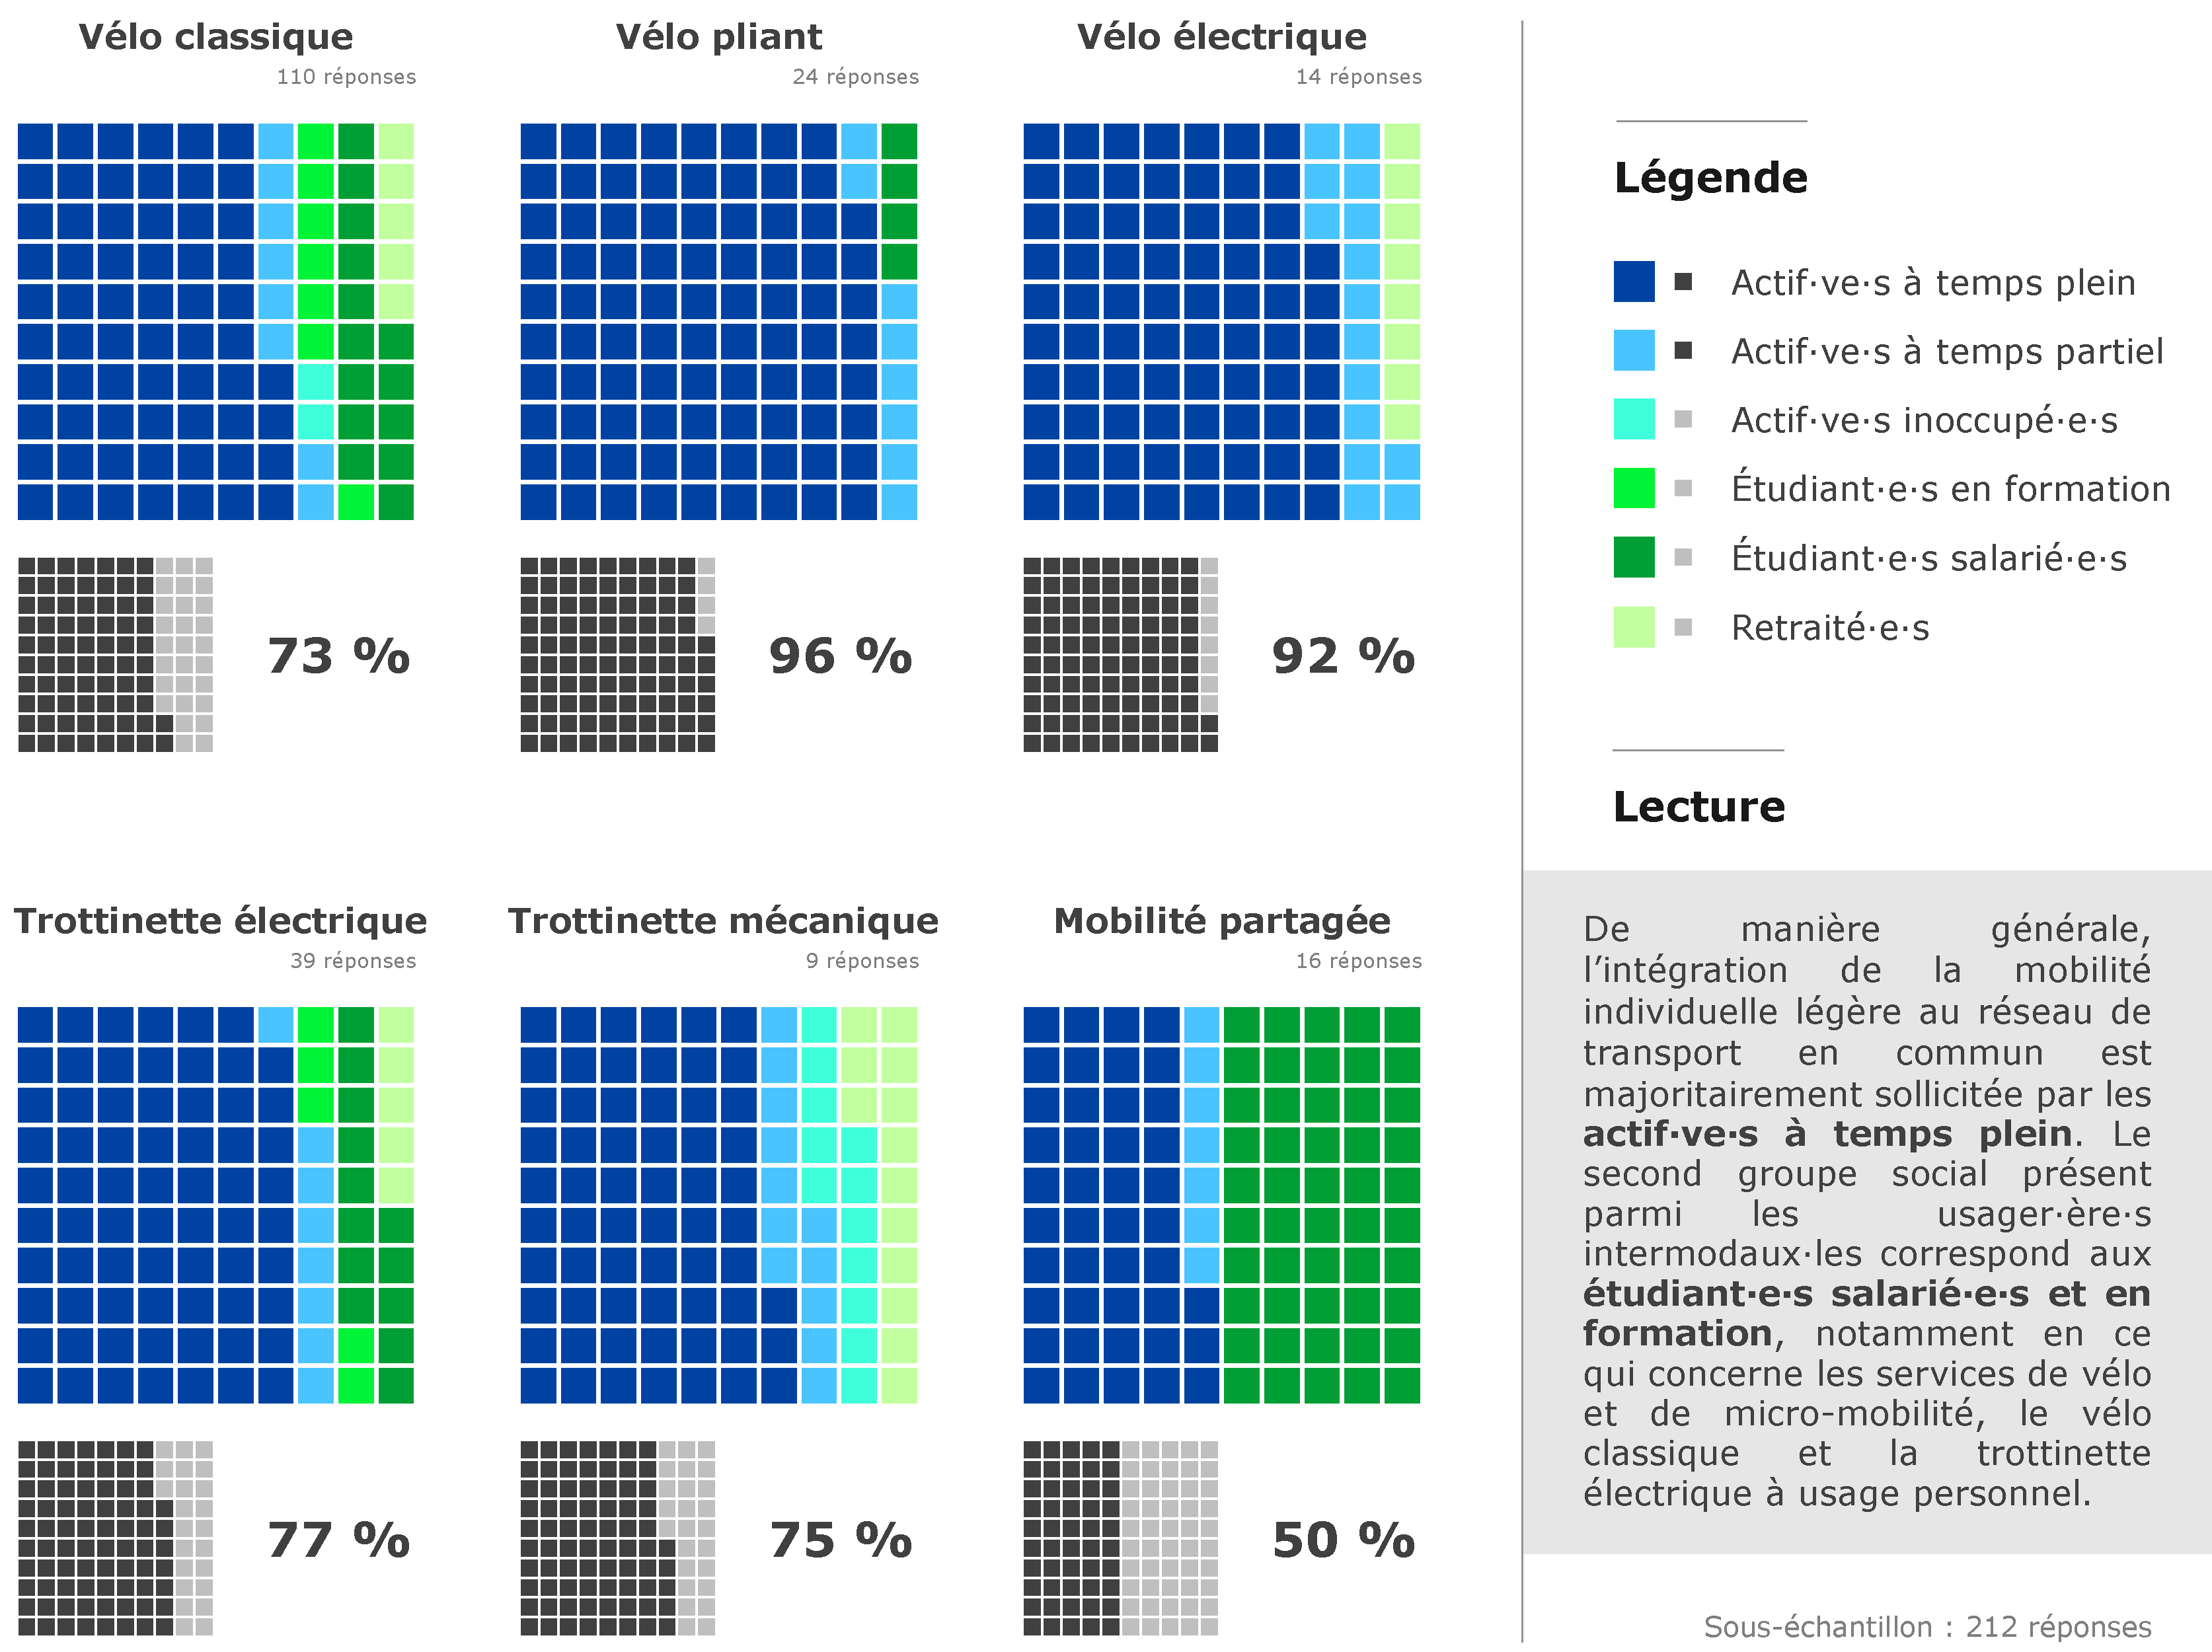
\includegraphics[width=1\columnwidth]{src/Figures/Chap-4/FR_Statut.pdf}}
        \vspace{5pt}
        \begin{flushleft}\scriptsize{
        Note~: un \Guillemets{pixel} correspond à 1~\% du sous-échantillon exploité.
        }\end{flushleft}
        \begin{flushright}\scriptsize{
        Auteur~: \textcolor{blue}{Dylan Moinse (2024)}
        }\end{flushright}
    \end{figure}

    % PCS - général
Afin d'explorer plus en détail la dimension socioprofessionnelle des cyclo-voyageur·se·s, nous avons intégré une question supplémentaire qui se rapporte à la \Guillemets{profession et catégorie socioprofessionnelle [à laquelle iels appartiennent ou ont appartenu] dernièrement} (voir l'\hyperref[annexes:structure-questionnaire-usagers]{annexe~\ref{annexes:structure-questionnaire-usagers}}, page~\pageref{annexes:structure-questionnaire-usagers}). En effet, la présence notable des actif·ve·s occupé·e·s parmi ces pratiques intermodales nous amène à examiner de plus près la stratification sociale au sein de cette population. L'analyse des \acrshort{PCS} indique une concentration significative de cadres et de professions intellectuelles supérieures, qui représentent 66~\% des personnes actives au questionnaire (109 réponses). Les employé·e·s forment le deuxième groupe le plus représenté avec 18~\% (29 réponses), tandis que les professions intermédiaires comptent pour 9~\% (15 réponses). En revanche, les artisan·e·s, commerçant·e·s et chef·fe·s d'entreprise ainsi que les ouvrier·ère·s représentent chacun·e 4~\% (6 réponses), signalant une moindre représentation de ces catégories dans l'usage intermodal de la mobilité légère. En effet, la proportion de cadres supérieur·e·s, déjà élevée parmi les usager·ère·s ferroviaires, s'avère encore plus significative dans le cadre de notre enquête sur les voyageur·se·s intermodaux·les. À l'inverse, les catégories professionnelles, telles que les ouvrier·ère·s et les artisan·e·s, y sont nettement sous-représentées (voir le \hyperref[table-chap4:capital-economique]{tableau \ref{table-chap4:capital-economique}}, page~\pageref{table-chap4:capital-economique}).%%Rédigé%%

    % PCS - modes et transition
La considération ciblée sur la proportion de cadres et de professions intellectuelles supérieures soutient l'hypothèse de leur poids significatif dans l'usage intermodal de la mobilité individuelle légère (voir l'\hyperref[fig-chap4:pcs]{illustration \ref{fig-chap4:pcs}}, page~\pageref{fig-chap4:pcs}), et plus particulièrement du vélo pliant (87~\%, 19 réponses). Cette tendance se poursuit avec le \acrshort{VAE} où 69~\% des utilisateur·rice·s appartiennent à cette catégorie (9 réponses), suivi·e·s de près par le vélo classique (69~\%, 55 réponses). En revanche, la part de ces professions chez les usager·ère·s de la \acrshort{TEP} est moins centrale, s'établissant à 49~\% (14 réponses). Il est à noter que la proportion d'employé·e·s recourant à la \acrshort{TEP} est accrue, atteignant 31~\% (9 réponses). La présence manifeste des cadres supérieur·e·s soulève une interrogation plus large sur les revenus des ménages, nous invitant ainsi à adopter une perspective qui dépasse la nomenclature des métiers, afin de mieux appréhender le capital économique des usager·ère·s intermodaux·les.%%Rédigé%%

    % Figure PCS
    \begin{figure}[h!]\vspace*{4pt}
        \caption{Professions et Catégories Socioprofessionnelles des cyclistes intermodaux·les selon le type de véhicule.}
        \label{fig-chap4:pcs}
        \centerline{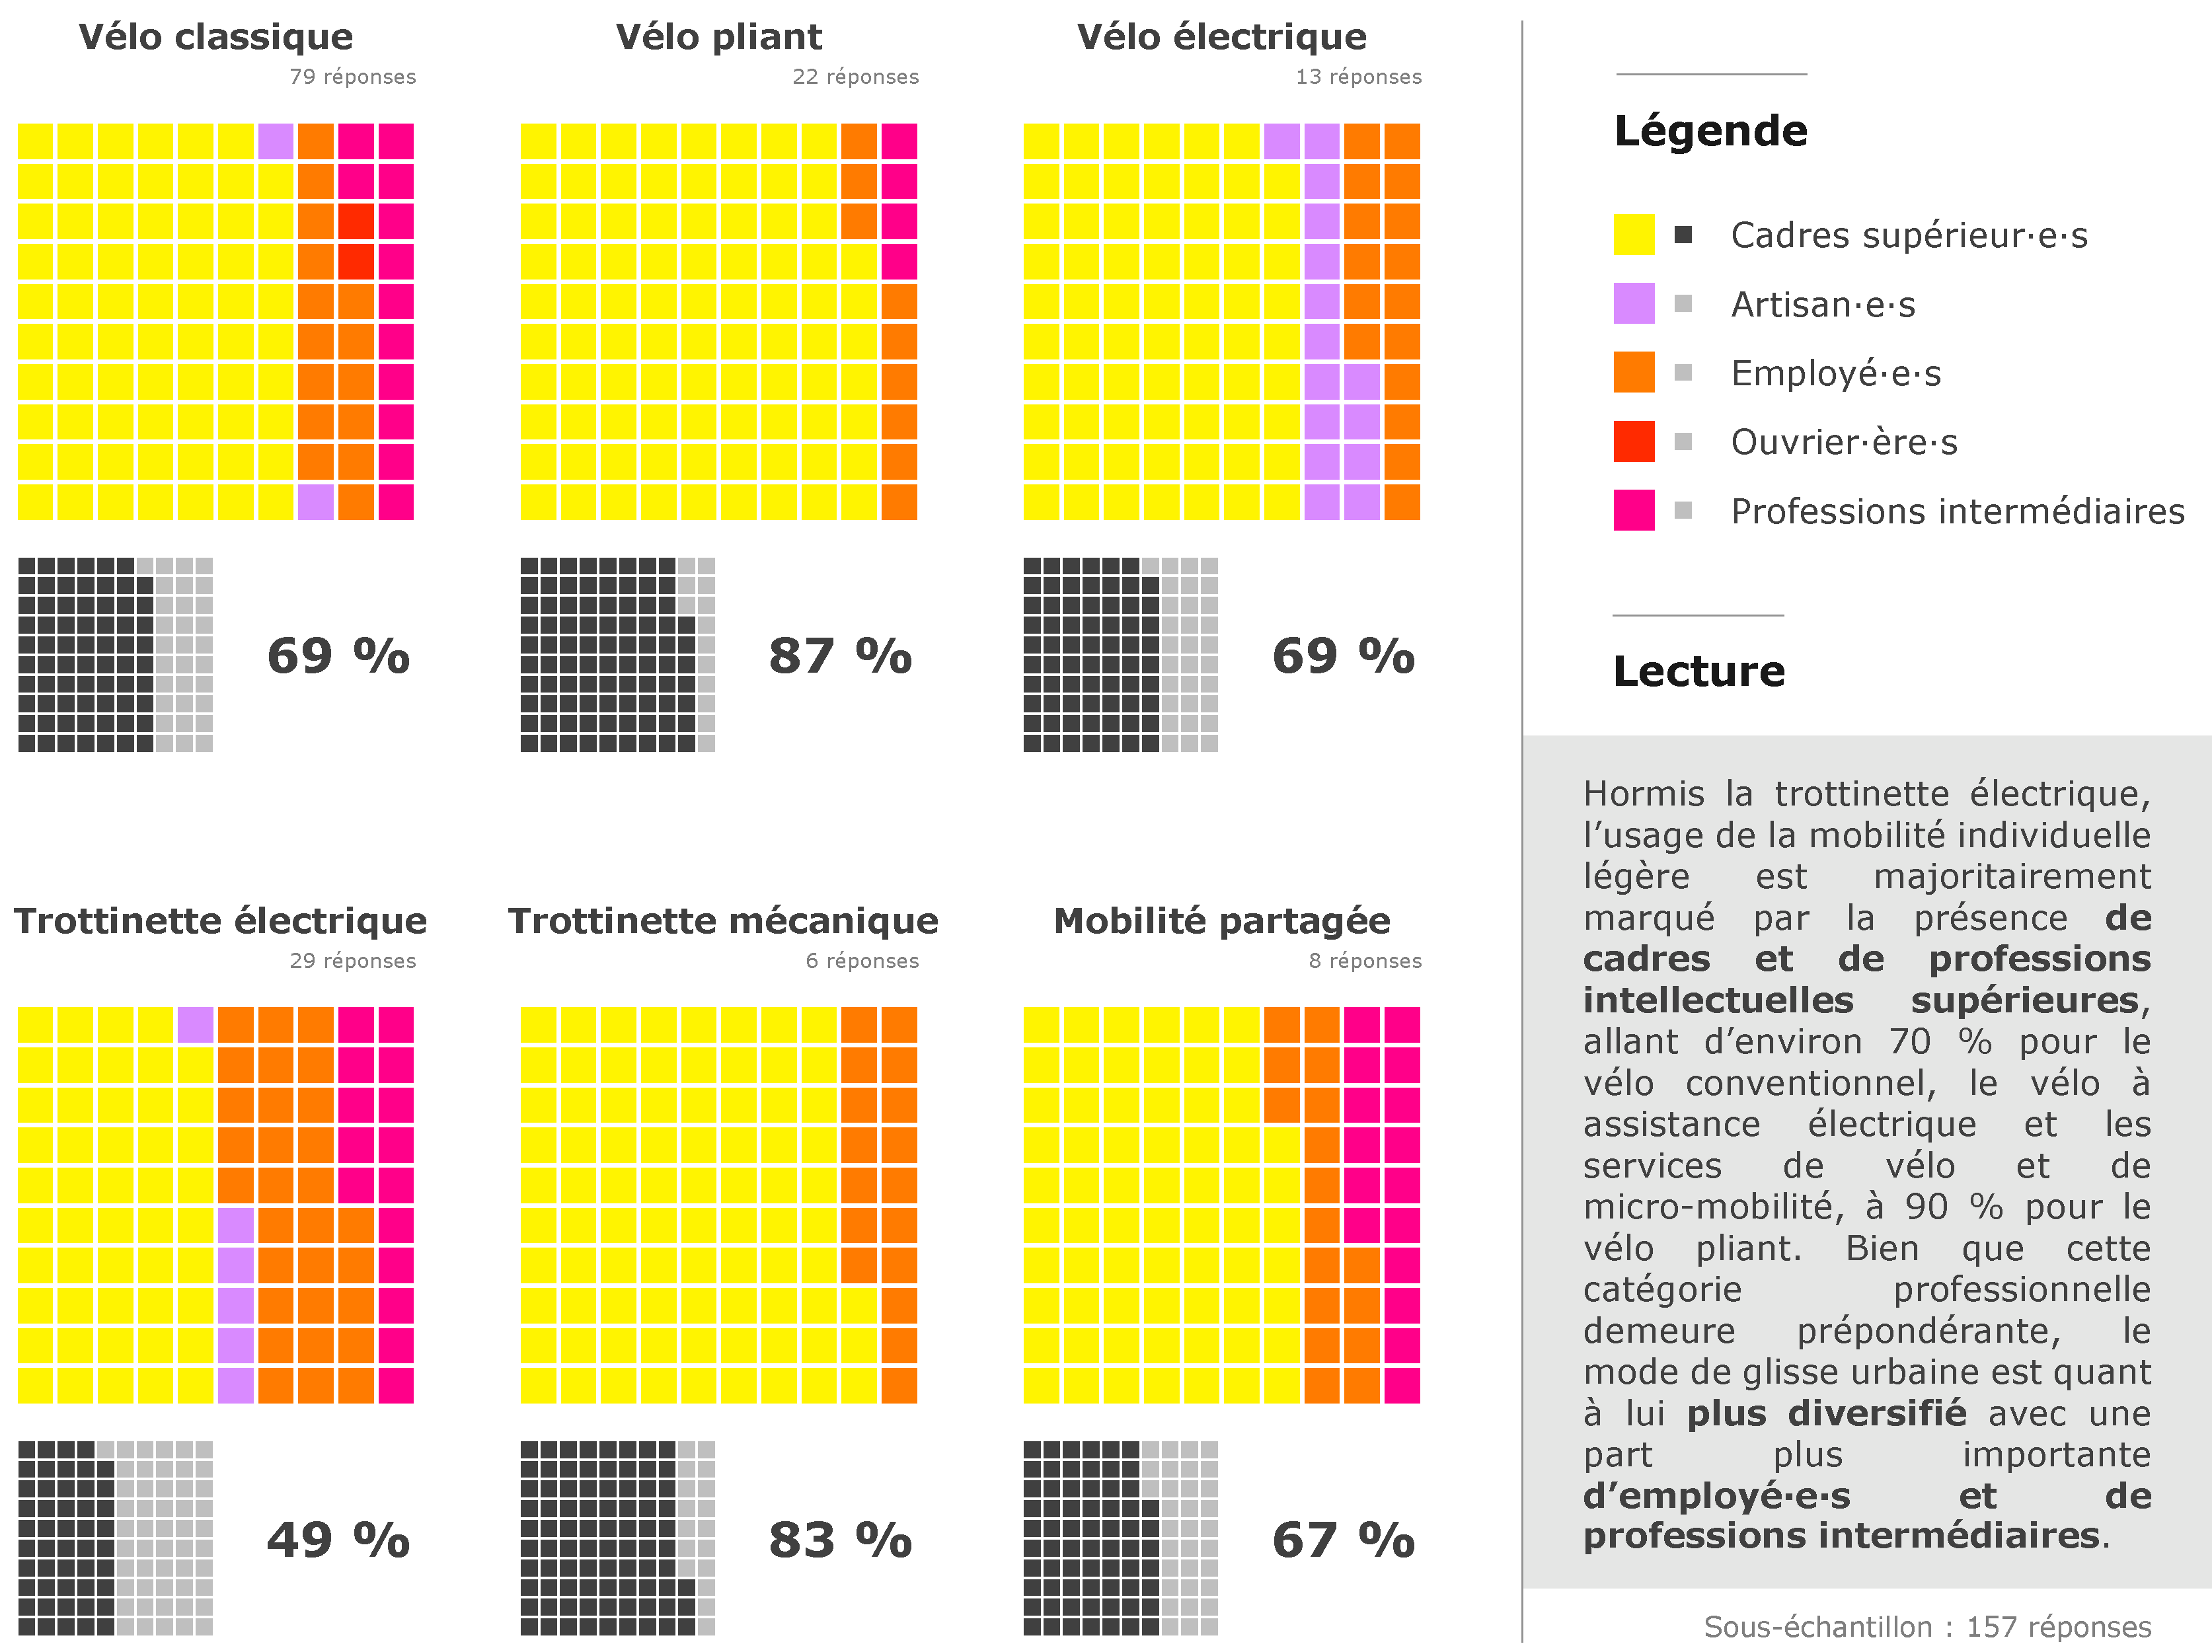
\includegraphics[width=1\columnwidth]{src/Figures/Chap-4/FR_PCS.pdf}}
        \vspace{5pt}
        \begin{flushleft}\scriptsize{
        Note~: un \Guillemets{pixel} correspond à 1~\% du sous-échantillon exploité.
        }\end{flushleft}
        \begin{flushright}\scriptsize{
        Auteur~: \textcolor{blue}{Dylan Moinse (2024)}
        }\end{flushright}
    \end{figure}

    % Littérature situation professionnelle + PCS + Transition
Une attention particulière a été portée sur la situation professionnelle des utilisateur·rice·s de la mobilité individuelle légère combinée, démontrant une influence majeure des actif·ve·s occupé·e·s et des étudiant·e·s, tandis que les retraité·e·s sont nettement sous-représenté·e·s. Cette distribution peu représentative de la population française soutient un corpus de recherches internationales ayant mis en évidence une distribution également inégalitaire \textcolor{blue}{\autocites[112]{quarshie_integrating_2007}[192]{sherwin_practices_2011}[21]{halldorsdottir_home-end_2017}{cervero_bike-and-ride_2013}[9]{jonkeren_bicycle-train_2021}[12]{pages_nouveaux_2021}}\index{Sherwin, Henrietta|pagebf}\index{Parkhurst, Graham|pagebf}\index{Robbins, Derek|pagebf}\index{Walker, Ian|pagebf}\index{Halldórsdóttir, Katrín|pagebf}\index{Nielsen, Otto Anker|pagebf}\index{Prato, Carlo Giacomo|pagebf}\index{Jonkeren, Olaf|pagebf}\index{Kager, Roland|pagebf}\index{Harms, Lucas|pagebf}\index{te Brömmelstroet, Marco|pagebf}\index{Quarshie, Magnus|pagebf}\index{Morrison, Gregory~M.|pagebf}\index{Rauch, Sébastien|pagebf}\index{Cervero, Robert|pagebf}\index{Caldwell, Benjamin|pagebf}\index{Cuellar, Jesus|pagebf}\index{Pages, Thibaud|pagebf}\index{Lammoglia, Adrien|pagebf}\index{Josselin, Didier|pagebf}. L'usage privilégié des services de mobilité par les étudiant·e·s est également documenté \textcolor{blue}{\autocites[215]{lin_built_2018}[8]{adnan_last-mile_2019}[3-4]{fearnley_patterns_2020}[12]{hu_examining_2022}[5]{cheng_comparison_2023}}\index{Lin, Jen-Jia|pagebf}\index{Zhao, Pengjun|pagebf}\index{Takada, Kazuyuki|pagebf}\index{Li, Shengxiao|pagebf}\index{Yai, Tetsuo|pagebf}\index{Chen, Chi-Hao|pagebf}\index{Adnan, Muhammad|pagebf}\index{Altaf, Shahbaz|pagebf}\index{Bellemans, Tom|pagebf}\index{Yasar, Ansar-ul-Haque|pagebf}\index{Shakshuki, Elhadi~M.|pagebf}\index{Hu, Songhua|pagebf}\index{Chen, Mingyang|pagebf}\index{Jiang, Yuan|pagebf}\index{Sun, Wei|pagebf}\index{Xiong, Chenfeng|pagebf}\index{Cheng, Long|pagebf}\index{Huang, Jie|pagebf}\index{Jin, Tanhua|pagebf}\index{Chen, Wendong|pagebf}\index{Li, Aoyong|pagebf}\index{Witlox, Frank|pagebf}\index{Fearnley, Nils|pagebf}\index{Johnsson, Espen|pagebf}\index{Berge, Siri Hegna|pagebf}.%%Rédigé%%

    % 4.2.1.2.
    \needspace{1\baselineskip} % Réserve de l'espace
\subsubsection*{Des revenus asymétriquement distribués
    \label{chap4:capital-economique-revenu}
    }

    % Revenu brut - général
La question relative à l'évaluation des revenus bruts mensuels du foyer a été posée. Le \acrfull{RDB}\footnote{
    Le \acrfull{RDB} constitue un indicateur économique reflétant la capacité financière d’un ménage après acquittement des impôts directs et intégration des diverses allocations et subventions publiques. Ce paramètre englobe non seulement les revenus nets mensuels issus de l'activité professionnelle et des biens possédés, mais aussi les prestations sociales perçues. Le \acrshort{RDB} offre ainsi une vision exhaustive des ressources disponibles pour un individu ou un ménage, destinées à la consommation, à l’investissement ou à l’épargne.
} moyen des répondant·e·s s'établit à 3~058~\euro, tandis que la médiane se situe à 2~850~\euro. Cet écart indique la présence de revenus relativement élevés parmi les participant·e·s, contribuant à une élévation de la moyenne. Comparativement, ce salaire moyen est inférieur au revenu brut moyen national de 3~250~\euro, toutefois, il dépasse la médiane nationale qui s'élève à 2~250~\euro, comme le montre le \hyperref[table-chap4:capital-economique]{tableau \ref{table-chap4:capital-economique}} (page~\pageref{table-chap4:capital-economique}). Dans l'analyse distributive des revenus basée sur une série cumulative classée par décile, il apparaît que le premier quartile (\(Q1\)) situe le seuil de revenu de trois quarts des répondant·e·s au-dessus de 1~750~\euro, tandis que le troisième quartile (\(Q3\)) indique qu'un quart des individus perçoit des revenus supérieurs à 4~050~\euro. Cette segmentation des \acrshort{RDB} met alors en évidence une distribution inégalement pondérée vers les tranches de revenu supérieures.%%Rédigé%%

    % Revenu brut - modes
L'analyse des revenus médians associés à l'intégration de la mobilité individuelle légère fait apparaître une médiane globale fixée à 2~850~\euro. Toutefois, des disparités marquées se manifestent lorsque nous examinons les données par mode de déplacement (voir l'\hyperref[fig-chap4:revenus]{illustration \ref{fig-chap4:revenus}}, page~\pageref{fig-chap4:revenus}). Par exemple, les utilisateur·rice·s du vélo pliant affichent un \acrshort{RDB} médian significativement supérieur, atteignant 4~050~\euro~(24 réponses), tandis que celleux du \acrshort{VAE} rapportent 3~400~\euro~(14 réponses). En revanche, les usager·ère·s de la trottinette mécanique et des systèmes de mobilité partagée présentent des revenus médians plus modestes, respectivement de 2~625~\euro~(9 réponses) et de 2~400~\euro~(16 réponses). Le vélo classique et la \acrshort{TEP} se positionnent dans une gamme intermédiaire, avec des revenus alignés sur la médiane déclarée. Plus largement, l'analyse de la distribution des revenus révèle un écart considérable entre les tranches de revenus les plus basses et les plus élevées, en particulier pour le vélopartage et le vélo classique.%%Rédigé%%

    % Figure Revenus
    \begin{figure}[h!]\vspace*{4pt}
        \caption{Diagrammes en boîte des revenus disponibles bruts des cyclistes intermodaux·les selon le type de véhicule.}
        \label{fig-chap4:revenus}
        \centerline{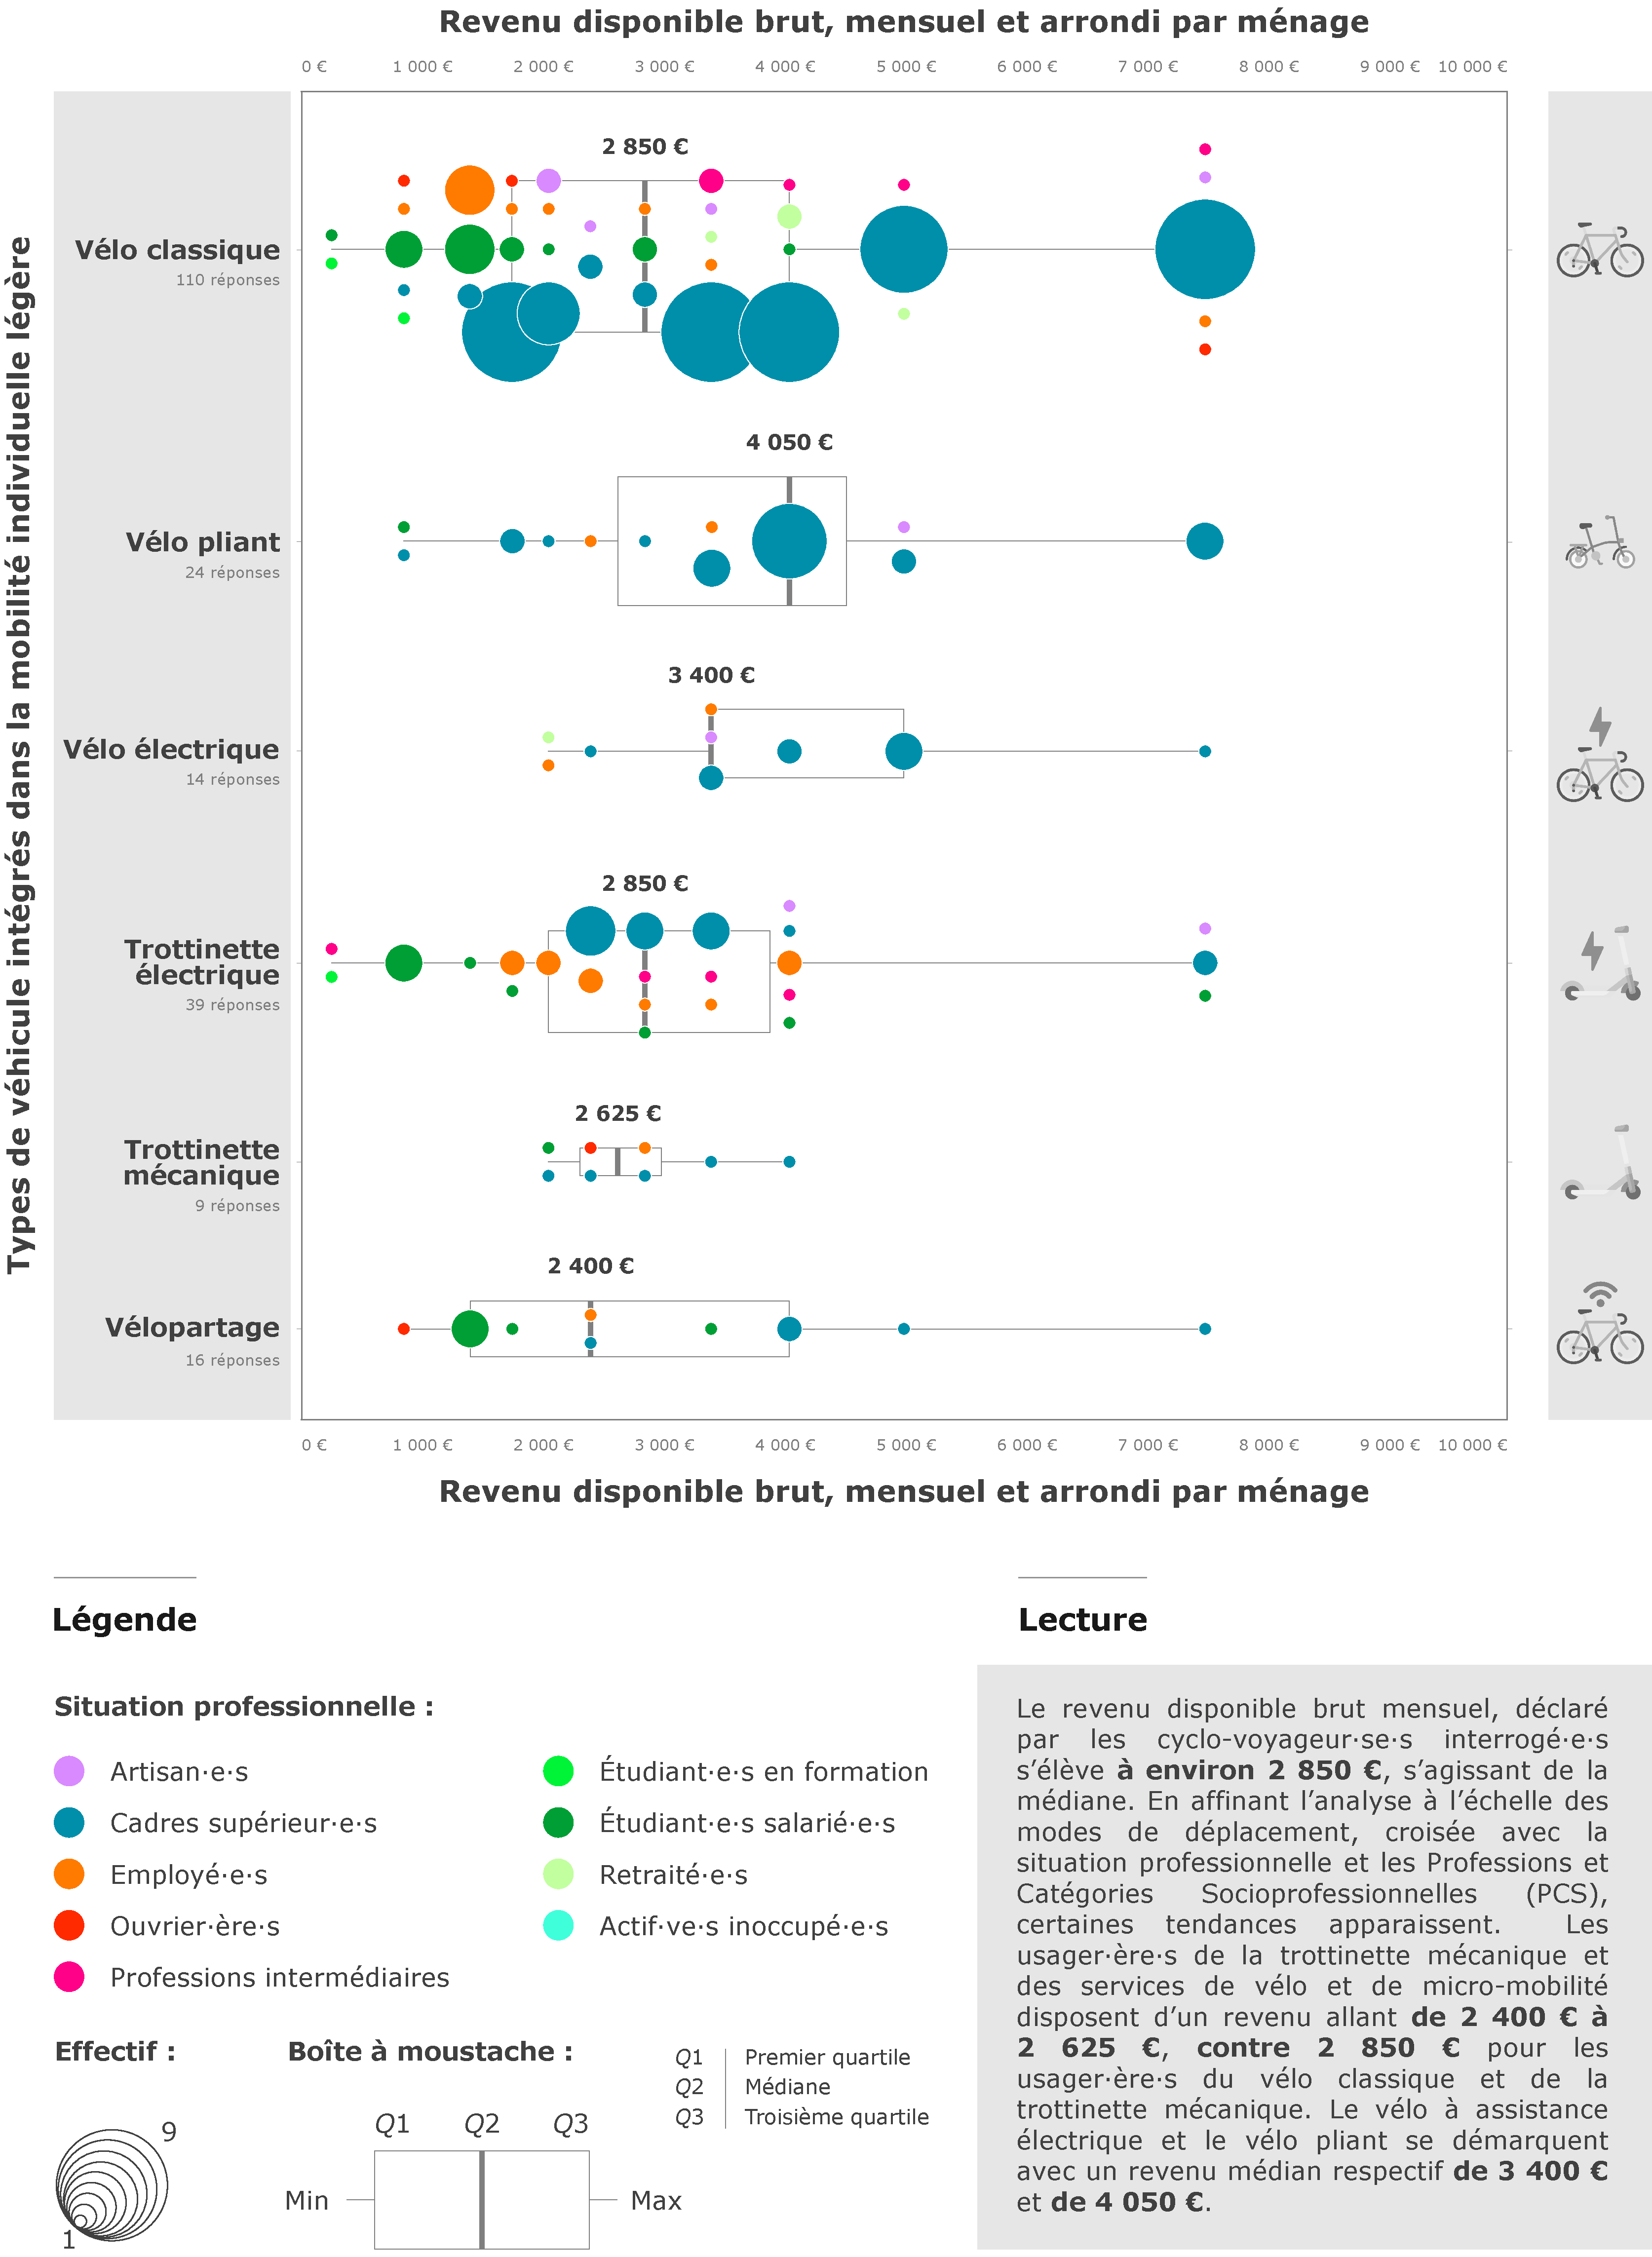
\includegraphics[width=1\columnwidth]{src/Figures/Chap-4/FR_Revenus.pdf}}
        \vspace{5pt}
        \begin{flushright}\scriptsize{
        Auteur~: \textcolor{blue}{Dylan Moinse (2024)}
        }\end{flushright}
    \end{figure}

    % Littérature situation revenus + Transition
Une attention particulière a été portée sur la situation professionnelle des utilisateur·rice·s de la mobilité individuelle légère combinée, démontrant une influence majeure des actif·ve·s occupé·e·s et des étudiant·e·s, tandis que les retraité·e·s sont nettement sous-représenté·e·s. Cette distribution peu représentative de la population française soutient un corpus de recherches internationales ayant mis en évidence une distribution également inégalitaire \textcolor{blue}{\autocites[112]{quarshie_integrating_2007}[192]{sherwin_practices_2011}[21]{halldorsdottir_home-end_2017}{cervero_bike-and-ride_2013}[9]{jonkeren_bicycle-train_2021}[12]{pages_nouveaux_2021}}\index{Sherwin, Henrietta|pagebf}\index{Parkhurst, Graham|pagebf}\index{Robbins, Derek|pagebf}\index{Walker, Ian|pagebf}\index{Halldórsdóttir, Katrín|pagebf}\index{Nielsen, Otto Anker|pagebf}\index{Prato, Carlo Giacomo|pagebf}\index{Jonkeren, Olaf|pagebf}\index{Kager, Roland|pagebf}\index{Harms, Lucas|pagebf}\index{te Brömmelstroet, Marco|pagebf}\index{Quarshie, Magnus|pagebf}\index{Morrison, Gregory~M.|pagebf}\index{Rauch, Sébastien|pagebf}\index{Cervero, Robert|pagebf}\index{Caldwell, Benjamin|pagebf}\index{Cuellar, Jesus|pagebf}\index{Pages, Thibaud|pagebf}\index{Lammoglia, Adrien|pagebf}\index{Josselin, Didier|pagebf}. L'usage privilégié des services de mobilité par les étudiant·e·s est également documenté \textcolor{blue}{\autocites[215]{lin_built_2018}[8]{adnan_last-mile_2019}[3-4]{fearnley_patterns_2020}[12]{hu_examining_2022}[5]{cheng_comparison_2023}}\index{Lin, Jen-Jia|pagebf}\index{Zhao, Pengjun|pagebf}\index{Takada, Kazuyuki|pagebf}\index{Li, Shengxiao|pagebf}\index{Yai, Tetsuo|pagebf}\index{Chen, Chi-Hao|pagebf}\index{Adnan, Muhammad|pagebf}\index{Altaf, Shahbaz|pagebf}\index{Bellemans, Tom|pagebf}\index{Yasar, Ansar-ul-Haque|pagebf}\index{Shakshuki, Elhadi~M.|pagebf}\index{Hu, Songhua|pagebf}\index{Chen, Mingyang|pagebf}\index{Jiang, Yuan|pagebf}\index{Sun, Wei|pagebf}\index{Xiong, Chenfeng|pagebf}\index{Cheng, Long|pagebf}\index{Huang, Jie|pagebf}\index{Jin, Tanhua|pagebf}\index{Chen, Wendong|pagebf}\index{Li, Aoyong|pagebf}\index{Witlox, Frank|pagebf}\index{Fearnley, Nils|pagebf}\index{Johnsson, Espen|pagebf}\index{Berge, Siri Hegna|pagebf}. Par ailleurs, une association positive notable entre les revenus des voyageur·se·s et leur inclination à opter pour la mobilité intermodale légère a été mise en évidence, comme l'illustrent divers travaux \textcolor{blue}{\autocites[321]{martin_evaluating_2014}[172]{yang_bike-and-ride_2014}[8]{ma_bicycle_2015}[7]{yang_empirical_2016}[55]{zhao_bicycle-metro_2017}[216]{lin_built_2018}[378]{ravensbergen_biking_2018}[15]{shelat_analysing_2018}[399]{bocker_bike_2020}[2~171]{chan_factors_2020}[184]{cao_e-scooter_2021}}\index{Shelat, Sanmay|pagebf}\index{Huisman, Raymond|pagebf}\index{Oort, Niels van|pagebf}\index{Chan, Kevin|pagebf}\index{Farber, Steven|pagebf}\index{Ravensbergen, Léa|pagebf}\index{Buliung, Ron|pagebf}\index{Mendonca, Meaghan|pagebf}\index{Garg, Naren|pagebf}\index{Yang, Liu|pagebf}\index{Chao, Li|pagebf}\index{Wang, Yuanqing|pagebf}\index{Martin, Elliot~W.|pagebf}\index{Shaheen, Susan~A.|pagebf}\index{Zhao, Pengjun|pagebf}\index{Li, Shengxiao|pagebf}\index{Yang, Min|pagebf}\index{Liu, Xinlu|pagebf}\index{Wang, Wei|pagebf}\index{Li, Zhibin|pagebf}\index{Zhao, Jingyao|pagebf}\index{Lin, Jen-Jia|pagebf}\index{Zhao, Pengjun|pagebf}\index{Takada, Kazuyuki|pagebf}\index{Li, Shengxiao|pagebf}\index{Yai, Tetsuo|pagebf}\index{Chen, Chi-Hao|pagebf}\index{Böcker, Lars|pagebf}\index{Anderson, Ellinor|pagebf}\index{Uteng, Tanu Priya|pagebf}\index{Throndsen, Torstein|pagebf}\index{Cao, Zhejing|pagebf}\index{Zhang, Xiaohu|pagebf}\index{Chua, Kelman|pagebf}\index{Yu, Honghai|pagebf}\index{Zhao, Jinhua|pagebf}\index{Ma, Ting|pagebf}\index{Liu, Chao|pagebf}\index{Erdoğan, Sevgi|pagebf}. Plus globalement, la surreprésentation des groupes sociaux mentionnés est corroborée par \textcolor{blue}{\textcite[101]{dobruszkes_is_2022}}\index{Dobruszkes, Frédéric|pagebf}\index{Chen, Chia-Lin|pagebf}\index{Moyano, Amparo|pagebf}\index{Pagliara, Francesca|pagebf}\index{Endemann, Peter|pagebf} qui ont constaté que, pour le \acrshort{TGV} en France, une majorité significative des usager·ère·s se compose de cadres supérieur·e·s et de personnes à revenus élevés, plus encore sur le segment Nord reliant les Hauts-de-France. À cela s'ajoutent la caractérisation d'un haut niveau de diplômes parmi les voyageur·se·s en \acrshort{TGV}, suggérant une association puissante entre le type de profession, le revenu et le niveau d'éducation chez les cyclo-voyageur·se·s, comme le soulignent \textcolor{blue}{\textcite[86]{zuo_incorporating_2021}}\index{Zuo, Ting|pagebf}\index{Wei, Heng|pagebf}\index{Chen, Na|pagebf}. Dès lors, cette section traitant du capital économique invite à se pencher sur le capital culturel de ces individus, afin d'affiner la détermination du profil socio-démographique des usager·ère·s intermodaux·les interrogé·e·s.%%Rédigé%%

    % 4.2.1.3.
    \needspace{1\baselineskip} % Réserve de l'espace
\subsubsection*{Un groupe social fortement qualifié
    \label{chap4:capital-culturel}
    }

    % Niveau de diplômes - général
À partir de la question relative au dernier diplôme obtenu, nous pouvons estimer le capital culturel des voyageur·se·s utilisant le vélo ou la micro-mobilité. D'après l'enquête, plus de 95~\% des répondant·e·s possèdent un diplôme de niveau supérieur, ce qui est nettement au-dessus de la moyenne nationale, établie à 43~\% (voir le \hyperref[table-chap4:capital-culturel]{tableau \ref{table-chap4:capital-culturel}}, page~\pageref{table-chap4:capital-culturel}). Environ 49~\% des personnes interrogées détiennent au moins un diplôme de niveau master, de types $7$ et $8$ selon le \acrfull{RNCP}\footnote{
    Le \acrfull{RNCP} est un registre officiel qui recense les qualifications et les certifications, accessibles par les formations professionnelles, reconnues par l'État. Celles-ci sont classées par niveau de qualification, allant du niveau $3$, pour le \acrshort{CAP} ou le \acrshort{BEP}, au niveau $8$ pour le doctorat et l'\acrshort{HDR}.
}, contre seulement 9,40~\% en moyenne pour l'ensemble de la population française. De plus, tandis que 13~\% des Français·e·s n'ont pas de diplôme ou de certificat d'études primaires, cette proportion tombe à 1~\% chez les voyageur·se·s intermodaux·les concerné·e·s, soulignant leur fort capital éducatif.%%Rédigé%%

    % Niveau de diplômes - modes
Le profil des usager·ère·s est marqué par des niveaux d’éducation différents entre les véhicules étudiés. Alors que 86~\% des répondant·e·s ont une licence, un master ou un doctorat (types $6$ à $8$, 180 réponses), 96~\% des utilisateur·rice·s du vélo pliant possèdent l'un de ces diplômes (23 réponses), contre 89~\% pour le vélo classique (93 réponses) et 74~\% pour la \acrshort{TEP} (29 réponses). Le véhicule électrique compte effectivement une proportion plus élevée d’usager·ère·s disposant d'un \acrshort{BTS}, d'un \acrshort{DEUG}, d'un \acrshort{DEUST}, d'un \acrshort{DUT} ou d'un baccalauréat comme plus haut niveau d’études.%%Rédigé%%

    % Tableau Capital culturel
% Tableau Capital culturel
%%Rédigé%%
    \begin{table}[h!]
    \centering
    \renewcommand{\arraystretch}{1.5}
    \resizebox{\columnwidth}{!}{
    \begin{tabular}{p{0.13\columnwidth}p{0.61\columnwidth}p{0.13\columnwidth}p{0.13\columnwidth}}
        %\hline
    \rule{0pt}{15pt} \small{\textcolor{blue}{{\textbf{Niveau}}}} & \small{\textcolor{blue}{{\textbf{Diplôme}}}} & \small{\textcolor{blue}{{\textbf{Enquête}}}} & \small{\textcolor{blue}{{\textbf{France}}}}\\
        \hline
\small{-} & \small{Aucun diplôme ou certificat d'études primaires} & \small{\textbf{0,96~\%}} & \small{12,50~\%}\\
\small{-} & \small{Brevet des collèges} & \small{\textbf{0,48~\%}} & \small{3,80~\%}\\
\small{$3$} & \small{\acrshort{CAP} ou \acrshort{BEP}} & \small{\textbf{0,48~\%}} & \small{22,40~\%}\\
\small{$4$} & \small{Baccalauréat} & \small{\textbf{3,35~\%}} & \small{18,80~\%}\\
\small{$5$} & \small{\acrshort{BTS}, \acrshort{DEUG}, \acrshort{DEUST} ou \acrshort{DUT}} & \small{\textbf{8,61~\%}} & \small{14,30~\%}\\
\small{$6$} & \small{Licence, licence professionnelle, \acrshort{BUT} ou Maîtrise} & \small{\textbf{36,84~\%}} & \small{18,80~\%}\\
\multirow{1.5}{*}{\small{$7$}} & \small{Master, diplôme d'études approfondies, d'études supérieures spécialisées ou d'ingénieur} & \multirow{1.5}{*}{\small{\textbf{47,85~\%}}} & \multirow{1.5}{*}{\small{8,30~\%}}\\
\small{$8$} & \small{Doctorat ou \acrshort{HDR}} & \small{\textbf{1,44~\%}} & \small{1,10~\%}\\
        \hline
        \end{tabular}}
    \caption{Niveau de qualification des cyclo-voyageur·se·s.}
    \label{table-chap4:capital-culturel}
        \vspace{5pt}
        \begin{flushleft}\scriptsize
        \textcolor{blue}{Lecture~:} comparativement à la moyenne nationale, les usager·ère·s sont bien plus diplômé·e·s, avec une prédominance des détenteur·rice·s d'une licence ou d'un master.
        \end{flushleft}
        \begin{flushright}\scriptsize{
        Jeux de données~: \textcolor{blue}{\textcite{insee_niveau_2021}}\index{Insee@\textsl{Insee}|pagebf}
        \\
        Auteur~: \textcolor{blue}{Dylan Moinse (2024)}
        }\end{flushright}
        \end{table}%%Rédigé%%

    % Littérature diplômes + transition
La prépondérance des diplômé·e·s parmi les usager·ère·s de la mobilité individuelle légère en intermodalité est confirmée par la littérature existante, qui associe fréquemment un haut niveau d'éducation à l'adoption de ces pratiques intermodales. Près de 86~\% des participant·e·s à notre étude détiennent un diplôme de l'enseignement supérieur, un chiffre qui s'aligne sur le taux de 85~\% mesuré par \textcolor{blue}{\textcite[15]{shelat_analysing_2018}}\index{Shelat, Sanmay|pagebf}\index{Huisman, Raymond|pagebf}\index{Oort, Niels van|pagebf}, \textcolor{blue}{\textcite[113]{heinen_multimodal_2014}}\index{Heinen, Eva|pagebf}\index{Bohte, Wendy|pagebf} et \textcolor{blue}{\textcite[11]{jonkeren_bicycle-train_2021}}\index{Jonkeren, Olaf|pagebf}\index{Kager, Roland|pagebf}\index{Harms, Lucas|pagebf}\index{te Brömmelstroet, Marco|pagebf} aux Pays-Bas, mais également sur les 75~\% et 74~\% relevés respectivement par \textcolor{blue}{\textcite[6, 8]{adnan_last-mile_2019}}\index{Adnan, Muhammad|pagebf}\index{Altaf, Shahbaz|pagebf}\index{Bellemans, Tom|pagebf}\index{Yasar, Ansar-ul-Haque|pagebf}\index{Shakshuki, Elhadi~M.|pagebf} en Belgique et par \textcolor{blue}{\textcite[103]{flamm_public_2014}}\index{Flamm, Bradley~J.|pagebf}\index{Rivasplata, Charles~R.|pagebf} aux États-Unis. Par comparaison avec les voyageur·se·s ferroviaires en France, où 63~\% des individus possèdent un niveau d'éducation supérieur au baccalauréat, il est clair que le capital éducatif des cyclistes intermodaux·les est sensiblement plus élevé, surpassant même celui des usager·ère·s du \acrshort{TGV} en France, où le taux s'élève à 70~\%.%%Rédigé%%

    % Transition
L'entrée par le capital économique met en exergue une nette surreprésentation des actif·ve·s occupé·e·s, en particulier des cadres supérieur·e·s aux revenus relativement élevés, parmi les cyclo-voyageur·se·s. Ce constat s'aligne sur les représentations sociales véhiculées~: celui du·de la cycliste empruntant le train et issu·e d'une catégorie socio-professionnelle favorisée. Au-delà de l'accessibilité cyclable et ferroviaire offerte par les combinaisons modales examinées, il convient également d'enquêter sur les capacités mobilitaires de ces usager·ère·s, à savoir la possession d'équipements de mobilité et leurs habitudes de déplacement.%%Rédigé%%

    % 4.2.3.
    \needspace{1\baselineskip} % Réserve de l'espace
\subsection{Portrait multimodal~: entre deux-roues et quatre-roues
    \label{chap4:capital-mobilite}
    }

    % Introduction
L'analyse du profil de mobilité des cyclo-voyageur·se·s vise à appuyer la diversité de leur capital mobilité, à savoir les ressources matérielles et les pratiques de mobilité dont iels disposent au quotidien. Cette section s'intéresse d'abord à la possession de véhicules au sein des foyers de ces usager·ère·s afin de déterminer si ces dernier·ère·s bénéficient d'une flexibilité de déplacement, au-delà des alternatives intermodales. En complément, nous allons explorer leurs habitudes de déplacement pour savoir s'iels tendent vers des pratiques multimodales ou s'iels se cantonnent à l'usage intermodal de la mobilité intermodale dans leurs déplacements quotidiens et occasionnels.%%Rédigé%%

    % 4.2.3.1.
    \needspace{1\baselineskip} % Réserve de l'espace
\subsubsection*{Une surreprésentation des ménages motorisés
    \label{chap4:capital-mobilite-equipement}
    }

    % Equipement en vélo
Parmi les répondant·e·s de l'enquête, 73~\% possèdent au moins un vélo. En excluant celleux qui utilisent un vélo personnel dans le cadre du questionnaire, nous observons que 47~\% des usager·ère·s déclarent en posséder un (50 réponses). Pour contextualiser, en 2019, environ 32~\% des ménages français étaient équipés d'au moins un vélo adulte utilisé depuis moins d'un an, selon les données du \textcolor{blue}{\textcite{commissariat_general_au_developpement_durable_combien_2022}}\index{Commissariat général au développement durable@\textsl{Commissariat général au développement durable}|pagebf}. Dès lors, les cyclistes intermodaux·les tendent à être plus souvent équipé·e·s d'un vélo. À titre d'exemple, parmi les utilisateur·rice·s de la \acrshort{TEP}, 46~\% possèdent également un vélo (18 réponses). Ce constat suggère que, même en disposant d'un vélo, ces individus privilégient l'\acrshort{EDP} pour leurs déplacements dans des contextes intermodaux. Par ailleurs, la moitié des utilisateur·rice·s d'un vélo ou d'une trottinette en libre-service en détient un (7 réponses), laissant supposer qu'iels optent pour ce système de partage pour faciliter leur connexion aux nœuds de transport en commun (voir l'\hyperref[fig-chap4:equipement]{illustration \ref{fig-chap4:equipement}}, page~\pageref{fig-chap4:equipement}).%%Rédigé%%

    % Taux de motorisation
L'examen des équipements de mobilité des répondant·e·s dévoile un taux de motorisation de 69~\% (149 réponses), à un niveau similaire à celui observé en France, estimé à environ 600 véhicules pour 1~000 habitant·e·s \textcolor{blue}{\autocite{insee_equipement_2020}}\index{Insee@\textsl{Insee}|pagebf}. Ce taux varie selon le mode de déplacement utilisé (voir l'\hyperref[fig-chap4:equipement]{illustration \ref{fig-chap4:equipement}}, page~\pageref{fig-chap4:equipement}). Les usager·ère·s de la mobilité partagée présentent le taux de motorisation le plus bas, avec 60~\% (9 réponses), suivi du vélo conventionnel à 65~\% et du vélo pliant à 71~\% (72 et 17 réponses). En opposition, les utilisateur·rice·s de la \acrshort{TEP} et du \acrshort{VAE}, qu'il soit pliant ou non, affichent un taux de motorisation parmi les plus élevés, s'élevant à 77~\% pour chacun de ces modes (30 et 10 réponses). Ces chiffres restent pour autant plus élevés que ceux observés par \textcolor{blue}{\textcite[362]{givoni_access_2007}}\index{Givoni, Moshe|pagebf}\index{Rietveld, Piet|pagebf} et \textcolor{blue}{\textcite[7]{yang_empirical_2016}}\index{Yang, Min|pagebf}\index{Liu, Xinlu|pagebf}\index{Wang, Wei|pagebf}\index{Li, Zhibin|pagebf}\index{Zhao, Jingyao|pagebf}, à hauteur de 49~\%.%%Rédigé%%

    % Figure Equipement
    \begin{figure}[h!]\vspace*{4pt}
        \caption{Équipement des cyclistes intermodaux·les, en vélos et voitures, selon le type de véhicule.}
        \label{fig-chap4:equipement}
        \centerline{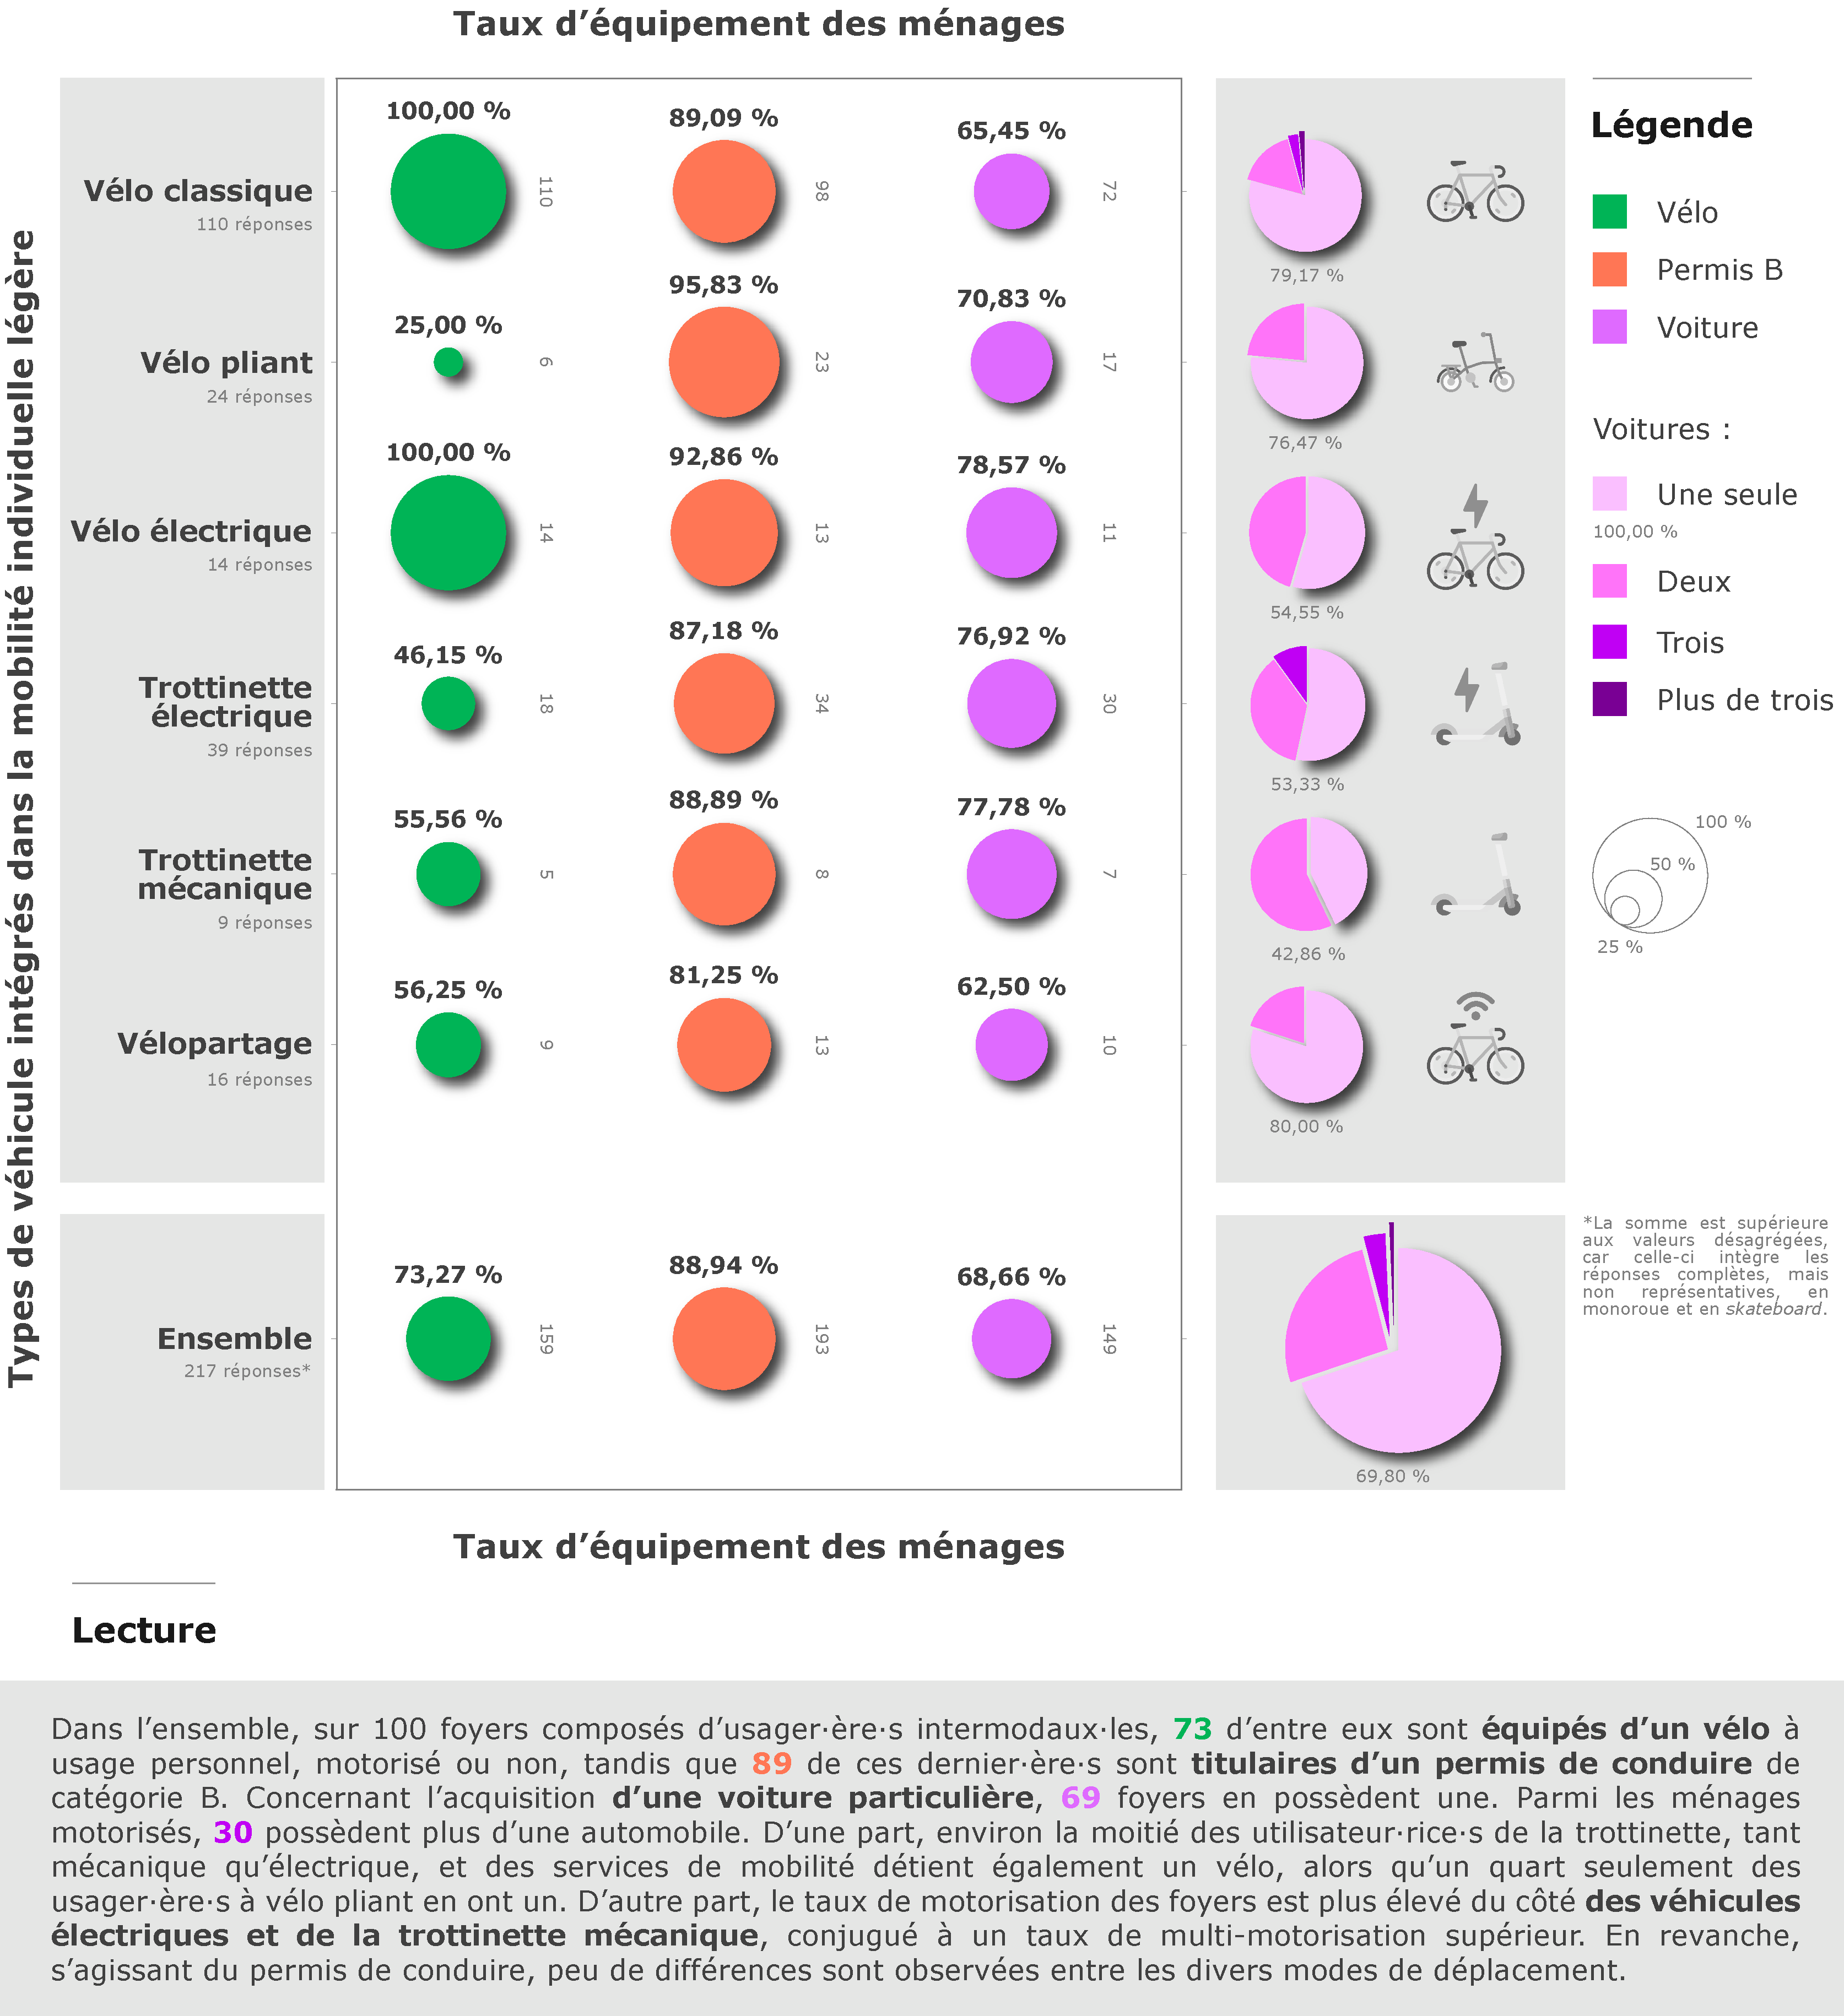
\includegraphics[width=1\columnwidth]{src/Figures/Chap-4/FR_Taux_motorisation.pdf}}
        \vspace{5pt}
        \begin{flushright}\scriptsize{
        Auteur~: \textcolor{blue}{Dylan Moinse (2024)}
        }\end{flushright}
    \end{figure}

    % Nombre de voitures
Dans une exploration plus détaillée des données, il apparaît que, pour l'ensemble des cyclo-voyageur·se·s, la possession moyenne s'établit à 0,93 voiture par foyer, tandis que celleux qui sont motorisé·e·s possèdent en moyenne 1,35 véhicule (voir l'\hyperref[fig-chap4:equipement]{illustration \ref{fig-chap4:equipement}}, page~\pageref{fig-chap4:equipement}). Parmi ces dernier·ère·s, 30~\% détiennent plus d'une voiture (45 réponses), et 4~\% possèdent trois voitures ou plus (6 réponses). Ainsi, la proportion de 34~\% des participant·e·s enquêté·e·s possédant plusieurs véhicules est assez proche du taux d'équipement de la population française en 2018, qui s'élève à 36~\% pour les ménages multi-motorisés \textcolor{blue}{\autocite{insee_equipement_2020}}\index{Insee@\textsl{Insee}|pagebf}. À ce titre, \textcolor{blue}{\textcite[22]{cheng_expanding_2018}}\index{Cheng, Yung-Hsiang|pagebf}\index{Li, Yi-Chun|pagebf} distinguent les propriétaires d'une voiture particulière qui tendent à être plus régulièrement des voyageur·se·s ayant recours au \acrshort{VLS}, de celleux disposant de plusieurs automobiles et moins enclin·e·s à adopter ces pratiques intermodales. Parmi les cyclistes motorisé·e·s interrogé·e·s, 21~\% des participant·e·s motorisé·e·s à vélo traditionnel et 24~\% à vélo pliant sont équipé·e·s d'au moins deux véhicules motorisés (15 et 4 réponses). La situation diffère cependant concernant le cas de l'électromobilité~: 47~\% des utilisateur·rice·s disposant d'une \acrshort{TEP} et 50~\% d'un \acrshort{VAE} sont quant à elleux multi-équipé·e·s (14 et 5 réponses). Cet écart pourrait indiquer que la mobilité individuelle légère électrique est privilégiée par des foyers motorisés, disposés à circuler sur le réseau routier et partageant des valeurs communes\footnote{
    Certaines recherches montrent que le vélo et la trottinette partagent plusieurs valeurs associées à l'\Guillemets{automobilité} \textcolor{blue}{\autocites[57-58]{urry_sociology_2000}[28]{urry_system_2004}}\index{Urry, John|pagebf}, notamment le sentiment de liberté, de flexibilité et d'indépendance ainsi que des éléments techniques comme l'infrastructure, qui caractérisent la conduite automobile. Ces ressources à la fois matérielles et symboliques attirent particulièrement les automobilistes désireux·ses de conserver ces avantages. La mobilité individuelle légère assure alors un excellent potentiel de report modal en étant le garant d'une transition vers un système de \Guillemets{vélomobilité} \textcolor{blue}{\autocite[492]{watson_how_2012}}\index{Watson, Matt|pagebf}.
}, soit pour substituer l'automobile dans des usages intermodaux, soit parce que les véhicules électriques ne réussissent pas à dissuader ces ménages de conserver la disponibilité d'une voiture privée.%%Rédigé%%

    % Permis de conduire
Pour explorer cette hypothèse, notre enquête a intégré une question relative à la possession du permis de conduire, croisée avec le taux de motorisation, pour identifier les profils des conducteur·rice·s, qu'iels soient actif·ve·s, occasionnel·le·s ou potentiel·le·s (voir l'\hyperref[fig-chap4:equipement]{illustration \ref{fig-chap4:equipement}}, page~\pageref{fig-chap4:equipement}). Globalement, une large majorité des répondant·e·s, soit 89~\%, détient un permis de conduire valide, de catégorie B\footnote{
    Le permis de conduire de catégorie B est le permis le plus courant qui autorise le·la titulaire à conduire des voitures particulières et d'autres véhicules légers, n'excédant pas 3,5 tonnes et 8 passager·ères.
} (193 réponses). La part de titulaires du permis de conduire parmi les voyageur·se·s ferroviaires ayant recours au vélo et à la micro-mobilité dépasse nettement celle au sein de la population française en âge de conduire, s'établissant à environ 76~\%. Cet enseignement rejoint la prédisposition observée sous d'autres latitudes des détenteur·rice·s du permis de conduire à se reporter davantage vers l'usage intermodal du vélo, en possession comme en libre-service \textcolor{blue}{\autocites[111]{bachand-marleau_much-anticipated_2011}[215]{lin_built_2018}[7]{hamidi_shaping_2020}}\index{Hamidi, Zahra|pagebf}\index{Zhao, Chunli|pagebf}\index{Lin, Jen-Jia|pagebf}\index{Zhao, Pengjun|pagebf}\index{Takada, Kazuyuki|pagebf}\index{Li, Shengxiao|pagebf}\index{Yai, Tetsuo|pagebf}\index{Chen, Chi-Hao|pagebf}\index{Bachand-Marleau, Julie|pagebf}\index{Larsen, Jacob|pagebf}\index{El-Geneidy, Ahmed~M.|pagebf}. Parmi les 68 participant·e·s non motorisé·e·s, 52 détiennent néanmoins ce titre. Inversement, parmi les 149 individus possédant un véhicule motorisé, 8 n'ont pas de permis, ce qui peut indiquer une utilisation du véhicule par d'autres membres du foyer ou une pratique potentielle de l'automobile en tant que passager·ère (\textsl{kiss-and-ride}). Nous devons ici en rester aux hypothèses, car notre questionnaire ne comportait pas la question de savoir si les enquêté·e·s avaient effectivement une voiture à leur disposition. Du fait des liens existants entre l'usage intermodal de la mobilité individuelle légère et l'équipement automobile, nous allons approfondir l'étude des pratiques de mobilité des cyclo-voyageur·se·s pour évaluer dans quelle mesure ces usager·ère·s adoptent un comportement multimodal ou s'iels se consacrent exclusivement à l'utilisation intermodale de la mobilité individuelle légère, tant dans leurs déplacements quotidiens qu'occasionnels.%%Rédigé%%

    % 4.2.3.2.
    \needspace{1\baselineskip} % Réserve de l'espace
\subsubsection*{\textsl{Pédaler}, \textsl{marcher} et \textsl{conduire}
    \label{chap4:capital-mobilite-habitudes}
    }

    % Habitudes de mobilité
En examinant les habitudes de mobilité des participant·e·s au moyen d'une échelle variant de \Guillemets{quotidiennement} à \Guillemets{jamais} pour chaque mode de déplacement, nous constatons que la plupart adoptent effectivement une approche multimodale. Ainsi, dans le cadre de leur mobilité quotidienne, 83~\% des sondé·e·s pratiquent la marche de façon régulière (180 réponses), 21~\% conduisent une voiture (46 réponses), et 4~\% sont passager·ère·s d'une voiture (8 réponses). Du côté des déplacements occasionnels, la marche concerne 12~\% des répondant·e·s (25 réponses), tandis que l'utilisation de la voiture atteint 27~\% en position de conducteur·rice (59 réponses) et 25~\% en \textsl{kiss-and-ride} (55 réponses). Le scooter et la moto, comme le taxi et le \acrshort{VTC}, concernent chacun 3~\% des individus, pour un total de 12 réponses. En focalisant notre attention sur les habitudes spécifiques des cyclo-voyageur·se·s motorisé·e·s, nous observons que 7~\% utilisent \Guillemets{quotidiennement} leur automobile (11 réponses), 22~\% \Guillemets{régulièrement} (34 réponses), 37~\% \Guillemets{occasionnellement} (57 réponses), 22~\% \Guillemets{rarement} (34 réponses) et 11~\% \Guillemets{jamais} (17 réponses).%%Rédigé%%

    % Discussion
Cette distribution dans la fréquence d'usage des différents modes de déplacement, en coexistence avec la mobilité individuelle légère et le transport public, démontre à quel point les usager·ère·s intermodaux·les n'observent pas ces pratiques de mobilité de manière exclusive, mais ont tendance à privilégier régulièrement la marche et occasionnellement l'automobile. Ce portrait des usager·ère·s alliant la mobilité individuelle légère et le transport public, mais cultivant également d'autres pratiques de mobilité, peut faire allusion à la thèse de \Guillemets{multimodalisation} des comportements développée par \textcolor{blue}{Anaïs} \textcolor{blue}{\textcite[16]{rocci_automobilite_2007}}\index{Rocci, Anaïs|pagebf}. Cette approche a le mérite de dépasser la simple notion de report modal, difficilement applicable au cas des cyclo-voyageur·se·s qui sont également automobilistes à l'occasion. Non sans rappeler l'exercice de prospective de \textcolor{blue}{Zygmunt} \textcolor{blue}{\textcite[7-28]{bauman_liquid_2000}}\index{Bauman, Zygmunt|pagebf}, qui compare les sociétés contemporaines à l'image d'une \Guillemets{vie liquide} (\textsl{liquid modernity}), caractérisée par des rythmes de vie marqués par un mouvement perpétuel et une flexibilité, symboles de liberté individuelle et s'opposant à l'idée de services rigides. À ce titre, il s'agit moins d'une transition vers un système de \Guillemets{vélomobilité} \textcolor{blue}{\autocite[492]{watson_how_2012}}\index{Watson, Matt|pagebf} que du passage d'un système d'\Guillemets{automobilité} \textcolor{blue}{\autocites[57-58]{urry_sociology_2000}[28]{urry_system_2004}}\index{Urry, John|pagebf} à celui de \Guillemets{multimobilité}\footnote{
    La multimobilité désigne l'utilisation de divers modes de déplacement pour se déplacer \textcolor{blue}{\autocite[10]{rocci_automobilite_2007}}\index{Rocci, Anaïs|pagebf}, un concept proche de celui de comodalité, introduit par le \textcolor{blue}{\textcite[6]{parlement_europeen_pour_2007}}\index{Parlement européen@\textsl{Parlement européen}|pagebf} dans ses politiques de transport, à distinguer de l'intermodalité. La multimobilité insiste sur la flexibilité et l'adaptabilité des individus qui optent pour diverses solutions de mobilité pour optimiser leurs voyages.
}.%%Rédigé%%

    % Transition
L'analyse a révélé que les cyclo-voyageur·se·s bénéficient non seulement d'un capital économique élevé et d'un statut social privilégié, mais aussi d'une certaine adaptabilité dans leurs choix de mobilité, en partie permise par la possession de véhicules automobiles. Toutefois, l'intégration de la mobilité individuelle légère est aussi influencée par des facteurs démographiques tels que l'âge et le genre, qui délimitent le champ des possibles en termes de mobilité. En étudiant l'accessibilité sous l'angle de l'inclusivité sociale comme cadre d'analyse, nous allons désormais examiner les disparités d'accès à la mobilité pour ce groupe social au prisme de sa démographie.%%Rédigé%%

    % 4.2.3.
    \needspace{1\baselineskip} % Réserve de l'espace
\subsection{Le voyageur intermodal, portrait typique du \textsl{jeune homme adulte}
    \label{chap4:demographie}
    }

    % Amorce
La commercialisation des trottinettes thermiques, puis l'avènement des modèles électriques, se sont traduits par l'élaboration de stratégies de vente ciblant une clientèle adulte et féminine. À cet égard, les campagnes publicitaires du début du XX\textsuperscript{e} siècle ont œuvré à transformer les représentations de la trottinette comme objet de loisirs, principalement destiné aux enfants, vers un outil d’émancipation des femmes participant à leur mobilité quotidienne \textcolor{blue}{\autocite{hemmings_look_2011}}\index{Hemmings@\textsl{Hemmings}|pagebf}. Cette évolution rappelle les mouvements pour les libertés individuelles qui, au tournant du siècle, s'étaient appuyés sur le vélo comme symbole de l'autonomisation des femmes \textcolor{blue}{\autocite[187]{heran_retour_2015}}\index{Héran, Frédéric|pagebf}. Il est pourtant reconnu, à l’heure actuelle, que l'utilisation de la trottinette électrique, comme du vélo, est caractérisée par un double effet d’âge et de genre. Parallèlement, certaines recherches soulèvent la question de l'accentuation des inégalités socio-démographiques avec le développement de la \acrshort{TEP}, même si \textcolor{blue}{\textcite[12]{curl_same_2020}}\index{Curl, Angela|pagebf}\index{Fitt, Helen|pagebf} apportent de la nuance à l'analyse, en montrant que la micro-mobilité réussit à séduire un public démographiquement plus diversifié que celui du vélo.%%Rédigé%%

    % Introduction
La littérature scientifique et technique reconnaît largement une distribution inégalitaire de l'usage monomodal de la mobilité individuelle légère, notamment sous l'angle des caractéristiques démographiques des utilisateur·rice·s en Europe et en Amérique du Nord \textcolor{blue}{\autocites[101]{handy_factors_2011}[8]{codina_built_2022}}\index{Handy, Susan~L.|pagebf}\index{Xing, Yan|pagebf}\index{Codina, Oriol|pagebf}\index{Maciejewska, Monika|pagebf}\index{Nadal, Jordi|pagebf}\index{Marquet, Oriol|pagebf}. Les études indiquent que la répartition selon l’âge et le genre dans la pratique du vélo est nettement déséquilibrée, reflétant des disparités marquées, contrairement à la marche et à l'usage des transports en commun où les femmes sont plus présentes \textcolor{blue}{\autocite[5-7]{pollard_gender_2017}}\index{Pollard, Tessa~M.|pagebf}\index{Wagnild, Janelle~M.|pagebf}. Ces inégalités sociales sont toutefois moins prononcées dans certains pays nord-européens comme les Pays-Bas, le Danemark et l'Allemagne, où une culture cycliste bien établie aurait permis d’atteindre une parité plus grande \textcolor{blue}{\autocites[81]{nelson_if_1997}[505]{pucher_making_2008}}\index{Nelson, Arthur~C.|pagebf}\index{Allen, David|pagebf}. Le Japon constitue également une exception, avec une pratique du vélo plus largement adoptée par les femmes, reflétant des normes socio-culturelles spécifiques \textcolor{blue}{\autocite[21-22]{lagadic_cycling_2022}}\index{Lagadic, Marion|pagebf}.%%Rédigé%%

    % Objectifs
Cependant, dans les régions où l'utilisation du vélo est moindre, les jeunes hommes tendraient à l'utiliser plus fréquemment que les femmes, comme à Barcelone \textcolor{blue}{\autocite[7]{codina_built_2022}}\index{Codina, Oriol|pagebf}\index{Maciejewska, Monika|pagebf}\index{Nadal, Jordi|pagebf}\index{Marquet, Oriol|pagebf}, en Nouvelle-Zélande \textcolor{blue}{\autocite[6]{shaw_beyond_2020}}\index{Shaw, Caroline|pagebf}\index{Russell, Marie|pagebf}\index{Keall, Michael|pagebf}\index{MacBride-Stewart, Sara|pagebf}\index{Wild, Kirsty|pagebf}\index{Reeves, Dory|pagebf}\index{Bentley, Rebecca|pagebf}\index{Woodward, Alistair|pagebf} ou aux États-Unis \textcolor{blue}{\autocite[513]{garrard_women_2012}}\index{Garrard, Jan|pagebf}\index{Handy, Susan~L.|pagebf}\index{Dill, Jennifer|pagebf}. Ces inégalités de genre dans l'utilisation du vélo ne peuvent être attribuées uniquement aux différences culturelles, mais doivent aussi être comprises au prisme des normes sociales liées à la mobilité et à l'\gls{espace public}, qui semblent avoir un impact disproportionné sur les personnes s’identifiant comme femmes. Dans cette perspective, cette sous-section vise à approfondir l'étude des pratiques intermodales, en particulier le rôle de la micro-mobilité qui a émergé récemment comme un mode de déplacement potentiellement moins inégalitaire.%%Rédigé%%

    % 4.2.3.1.
    \needspace{1\baselineskip} % Réserve de l'espace
\subsubsection*{De (\textsl{jeunes}) \textsl{adultes} adeptes de ces combinaisons modales
    \label{chap4:demographie-age}
    }

    % Âge observation - général
D'après les relevés effectués dans les neuf gares enquêtées, l'âge moyen des usager·ère·s est relativement similaire à celui des voyageur·se·s ferroviaires en général. L'analyse statistique indique que 71~\% des utilisateur·rice·s de la mobilité individuelle légère observé·e·s sont classifié·e·s comme \Guillemets{adultes} (733 observations), contre 63~\% (9~772 observations) dans le groupe général. Les \Guillemets{jeunes adultes} représentent le deuxième groupe d'âge présent parmi la population étudiée, avec 23~\% (242 observations), en comparaison avec 30~\% pour l'ensemble de l'échantillon (4~641 observations). Les \Guillemets{personnes âgées} constituent quant à elles 6~\% des individus recensés, concernant le sous-échantillon comme l'ensemble de la population (60 et 962 observations). Enfin, aucun \Guillemets{enfant} n'a été observé utilisant un vélo ou une option de micro-mobilité lors des séances d'observation, alors que cette catégorie se rapproche de 0~\% des voyageur·se·s ferroviaires (60 observations). Néanmoins, ces résultats sont probablement biaisés, étant donné que la constitution de l'échantillon dépend de la temporalité des séances d'observation, mises en application au cours des heures de pointe, capturant essentiellement les mobilités pendulaires.%%Rédigé%%

    % Âge questionnaire - général
Le questionnaire utilisé pour cette étude corrige alors ce biais méthodologique~–~cette enquête intègre \textsl{a priori} une plus grande diversité de cyclo-voyageur·se·s \Guillemets{invisibilisés}, soit en dehors des horaires d'affluence, soit parmi celleux stationnant leur véhicule~–~tout en fournissant des détails enrichissants sur les pratiques de mobilité des cyclo-voyageur·se·s en fonction de leur âge (voir l'\hyperref[fig-chap4:pyramide-age]{illustration \ref{fig-chap4:pyramide-age}}, page~\pageref{fig-chap4:pyramide-age}). Globalement, l'âge moyen des participant·e·s est de 36 ans, avec une médiane de 33 ans (209 réponses). La répartition par âge montre que seul 1~\% des répondant·e·s ont moins de 18 ans (3 réponses), que 40~\% ont moins de 30 ans (84 réponses), et que 6~\% ont plus de 60 ans (12 réponses).%%Rédigé%%

    % Âge observation - modes
Les groupes d'âge ne bénéficient pas de la même représentation au cœur de cet éventail de véhicules, s'agissant principalement de la \acrshort{TEP} qui attire davantage de jeunes usager·ère·s et du vélo ~–~un vélo classique, pliant et, ou bien, électrique~–, prisé de manière accrue par les individus plus âgés. Alors que les \Guillemets{adultes} constituent 71~\% du sous-échantillon des cyclistes intermodaux·les observé·e·s, cette proportion grimpe à 85~\% pour les utilisateur·rice·s du vélo, sous toutes ses formes (68 observations), et chute à 58~\% pour le monoroue et le \textsl{skateboard}, au bénéfice des \Guillemets{jeunes adultes} (7 observations). Plus en détail, le vélo se caractérise par une surreprésentation des \Guillemets{personnes âgées}, entre 9~\% et 10~\% (23 et 9 observations). En revanche, la \acrshort{TEP} et les autres formes de micro-mobilité électrique font nettement plus de place aux \Guillemets{jeunes adultes}, représentant entre 30~\% et 42~\% des usager·ère·s (99 et 7 observations).%%Rédigé%%

    % Âge questionnaire - modes
Ces enseignements sont appuyés par les données recueillies via le questionnaire, qui apportent une meilleure précision selon le type de véhicule et l'âge déclarés des répondant·e·s. De façon similaire, les utilisateur·rice·s du vélo classique et du vélo pliant appartiennent à des tranches d'âge plus avancées, avec une médiane à 42 et à 44 ans (105 et 24 réponses). S'ensuivent les véhicules électriques, composés du monoroue, du \textsl{skateboard}, du \acrshort{VAE} et de la \acrshort{TEP}, dont l'âge médian des usager·ère·s se situe entre 36 et 39 ans (4, 12 et 39 réponses). En dernière position, la trottinette mécanique ainsi que les services de vélo et de micro-mobilité séduisent un public plus jeune, ayant un âge médian de 29 et de 32 ans (9 et 16 réponses).%%Rédigé%%

    % Figure Pyramide âges
    \begin{figure}[h!]\vspace*{4pt}
        \caption{Pyramide des âges des cyclistes intermodaux·les, croisée au type de véhicule.}
        \label{fig-chap4:pyramide-age}
        \centerline{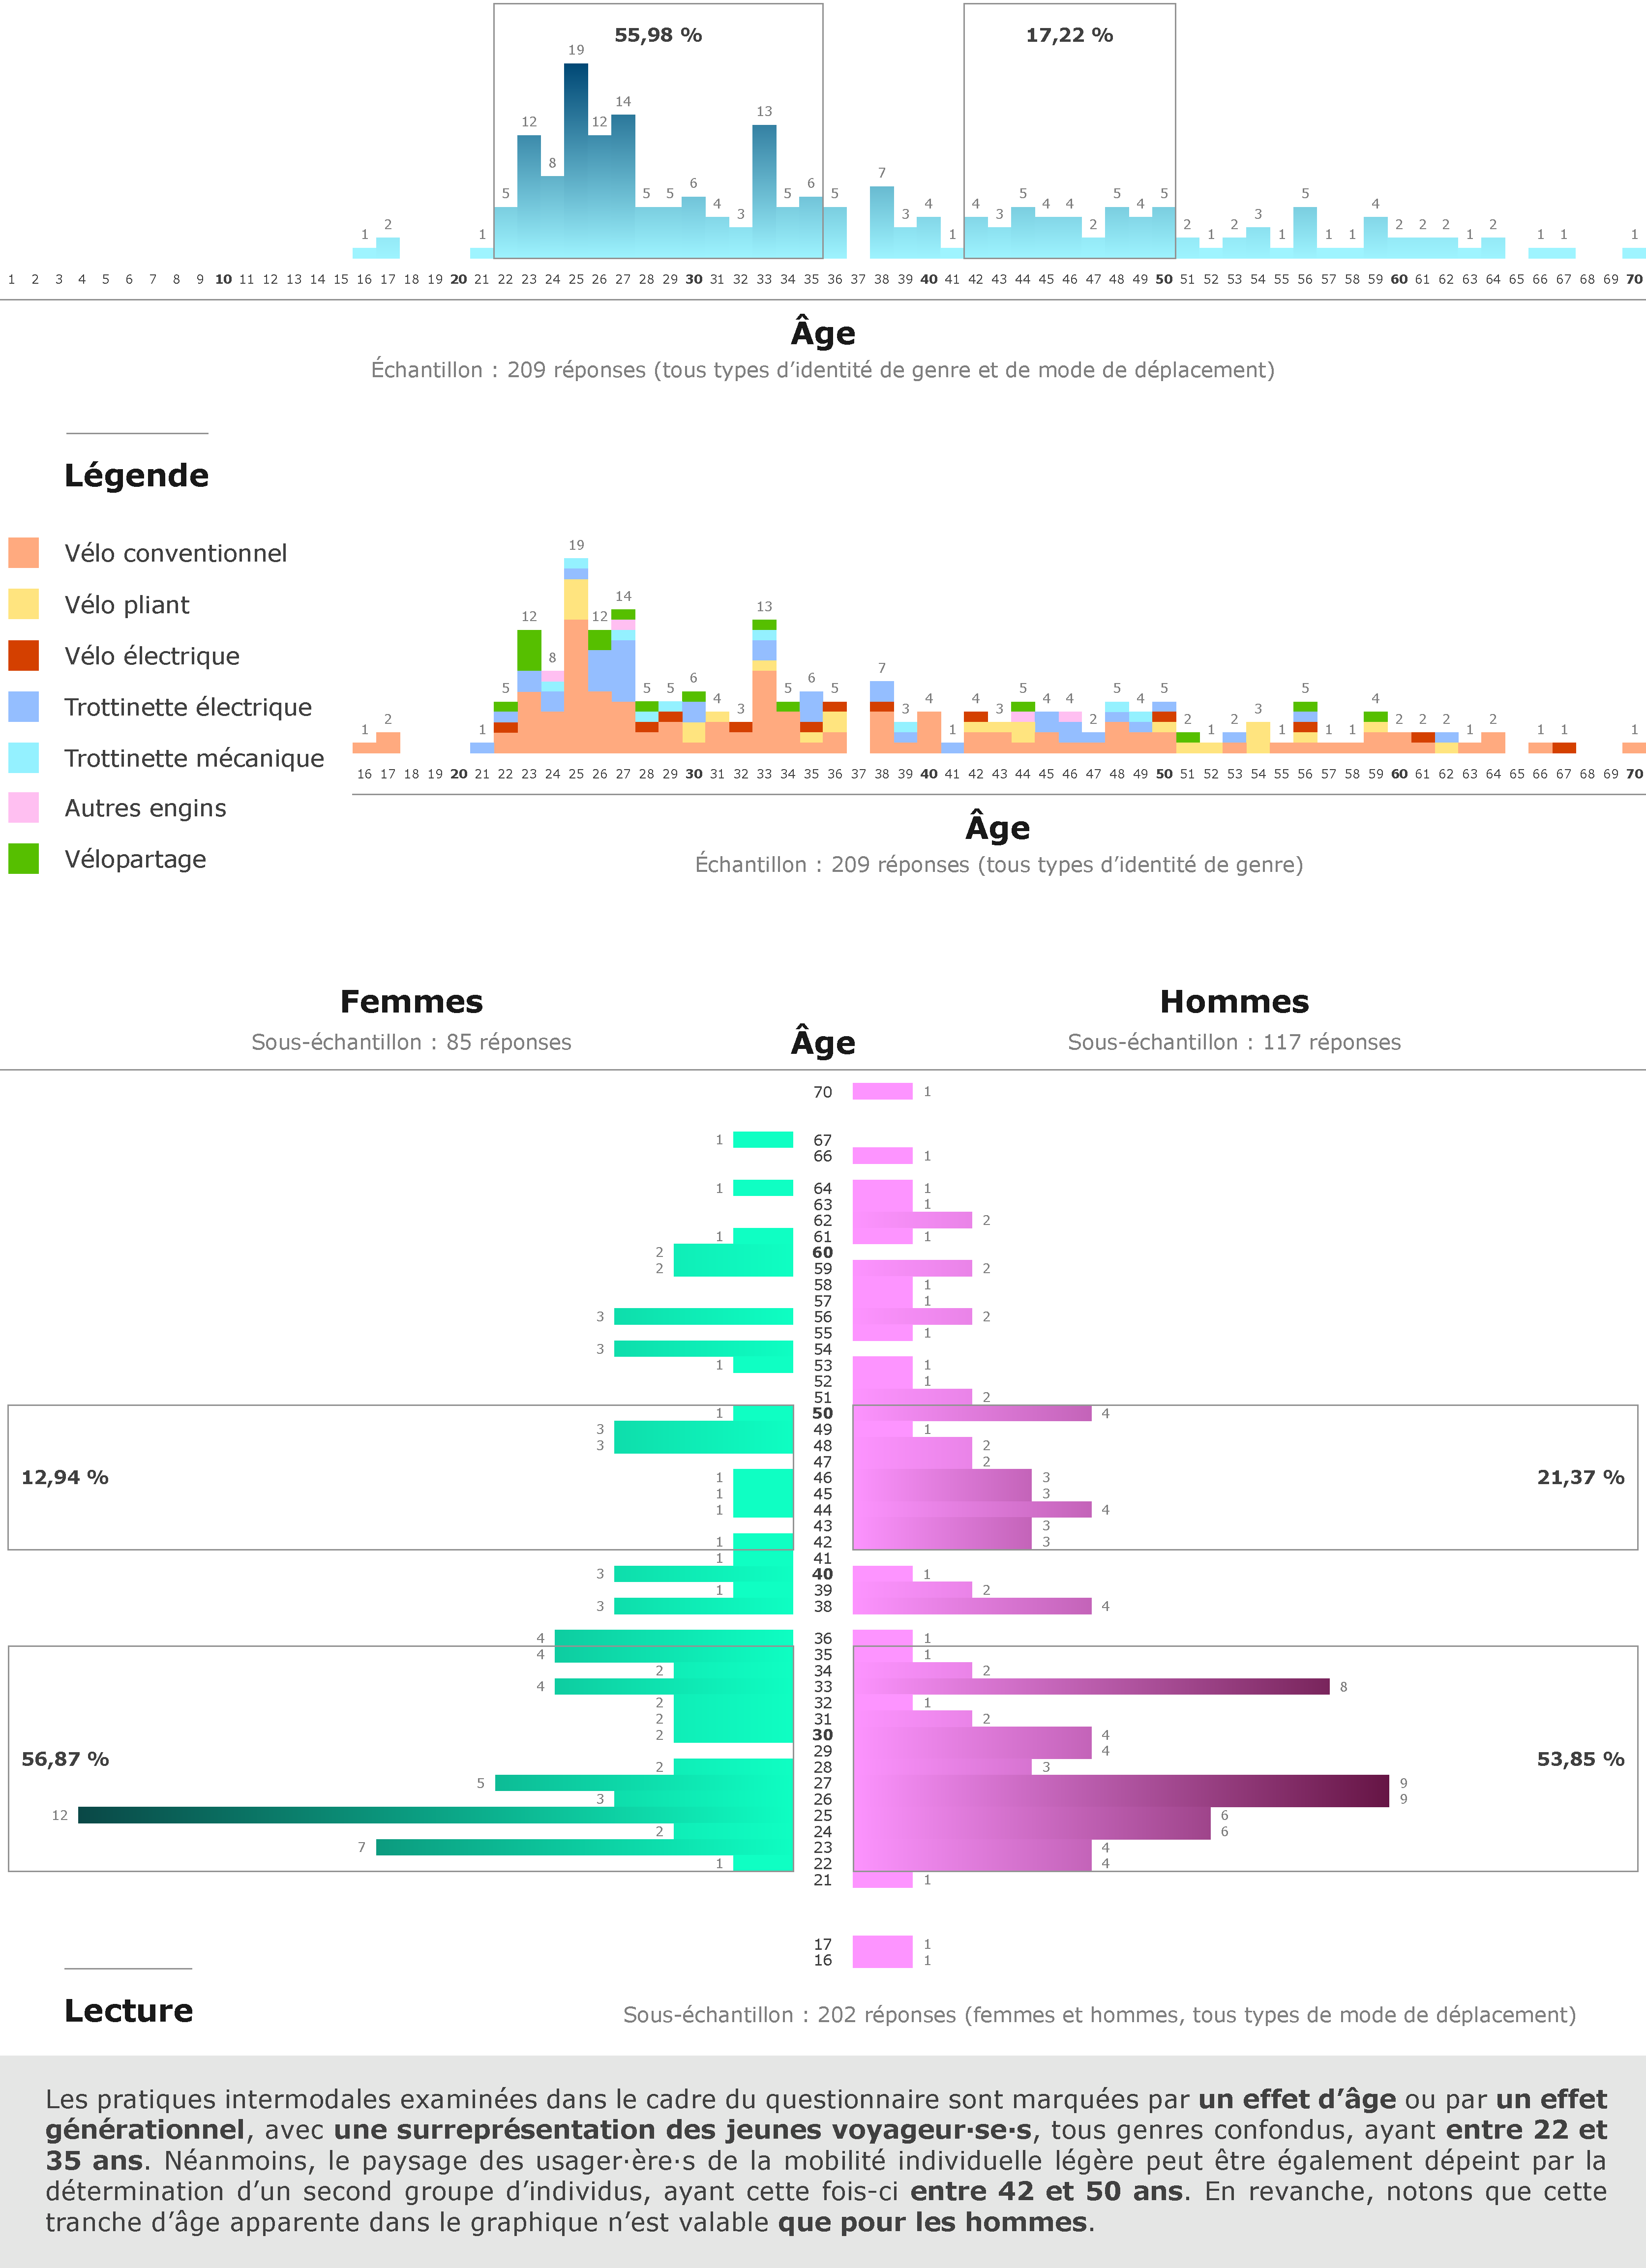
\includegraphics[width=1\columnwidth]{src/Figures/Chap-4/FR_Pyramide_age.pdf}}
        \vspace{5pt}
        \begin{flushright}\scriptsize{
        Auteur~: \textcolor{blue}{Dylan Moinse (2024)}
        }\end{flushright}
    \end{figure}

    % Second pic
Globalement, le segment d'âge de 22 à 35 ans rassemble la majorité des usager·ère·s intermodaux·les de la mobilité individuelle légère (56~\%, 117 réponses). Cela dit, il reste à signaler un pic secondaire parmi les cyclo-voyageur·se·s âgé·e·s de 42 à 50 ans (17~\%, 36 réponses). Ce constat concorde avec la segmentation de la clientèle de la \acrshort{TEFF} en Allemagne, telle que décrite par \textcolor{blue}{\textcite[4]{degele_identifying_2018}}\index{Degele, Jutta|pagebf}\index{Gorr, Anna|pagebf}\index{Haas, Katja|pagebf}\index{Kormann, Dimitri|pagebf}\index{Krauss, Sascha|pagebf}\index{Lipinski, Paulina|pagebf}\index{Tenbih, Muhammet|pagebf}\index{Koppenhoefer, Christine|pagebf}\index{Fauser, Jan|pagebf}\index{Hertweck, Dieter|pagebf}, influencée par un second pic d'utilisateur·rice·s âgé·e·s entre 45 et 50 ans et parcourant de plus longues distances en moyenne. Il apparaît donc que les tranches d'âge correspondant aux plus jeunes et aux seniors sont principalement sous-représentées par rapport aux voyageur·se·s ferroviaires et à la démographie générale de la population française.%%Rédigé%%

    % Littérature technique
En nous référant aux tranches d'âge des voyageur·se·s en gare \textcolor{blue}{\autocite{sncf_repartition_2017}}\index{SNCF@\textsl{SNCF}|pagebf}, nous pouvons effectivement retenir que les groupes d'âge les moins représentés au sein de notre sous-population sont les moins de 19 ans (1~\% contre 14~\%), tout comme les plus de 60 ans (6~\% contre 15~\%), tandis que la part des 20 à 39 ans est significative (64~\% contre 40~\%). Au regard de l'ensemble de la population \textcolor{blue}{\autocite{insee_age_2022}}\index{Insee@\textsl{Insee}|pagebf}, les moins de 19 ans (1~\% contre 23~\%) et les plus de 65 ans (1~\% contre 22~\%) demeurent marginalisé·e·s. En revanche, les intervalles les plus représentés restent les 20 à 34 ans (54~\% contre 17~\%) et, dans une moindre mesure, les 35 à 49 ans (25~\% contre 19~\%).%%Rédigé%%

    % Littérature scientifique
À la lumière des connaissances accumulées dans la littérature scientifique, nous avons démontré que, si le vélo et, plus encore, la micro-mobilité sont fréquemment privilégiés par les jeunes usager·ère·s en monomodalité \textcolor{blue}{\autocites[3]{winters_who_2019}[6]{bielinski_electric_2020}[4, 11]{gioldasis_risk-taking_2021}[13]{speak_scooter_2023}[200]{yang_shared_2024}}\index{Bieliński, Tomasz|pagebf}\index{Ważna, Agnieszka|pagebf}\index{Yang, Wencui|pagebf}\index{Jafarzadehfadaki, Mostafa|pagebf}\index{Yan, Xiang|pagebf}\index{Zhao, Xilei|pagebf}\index{Jin, Xia|pagebf}\index{Frolich, Daniel|pagebf}\index{Sisiopiku, Virginia~P.|pagebf}\index{|pagebf}\index{Speak, Anna|pagebf}\index{Taratula-Lyons, Monique|pagebf}\index{Clayton, William|pagebf}\index{Shergold, Ian|pagebf}\index{Gioldasis, Christos|pagebf}\index{Christoforou, Zoi|pagebf}\index{Seidowsky, Régine|pagebf}\index{Winters, Meghan|pagebf}\index{Hosford, Kate|pagebf}\index{Javaheri, Sana|pagebf}, leur emploi comme solution chaînante est nuancé par un élargissement du spectre démographique aux adultes. D'après notre étude de l'enquête par questionnaire conduite en Provence-Alpes-Côte d'Azur, nous avons pu identifier une surreprésentation des 25 à 34 ans parmi les utilisateur·rice·s de la \acrshort{TEP}, atteignant 28~\% contre 16~\% pour l'ensemble des passager·ère·s du \acrshort{TER}, avec un second pic pour les 45 à 54 ans \textcolor{blue}{\autocite[183]{moinse_intermodal_2022}}\index{Moinse, Dylan|pagebf}\index{Goudeau, Matthieu|pagebf}\index{L'Hostis, Alain|pagebf}\index{Leysens, Thomas|pagebf}. De surcroît, les moins de 17 ans et les plus de 55 ans sont moins présent·e·s, tandis que l'usage intermodal du vélo classique est plus fréquent chez les 35 à 44 ans. L'identification d'un profil de cyclo-voyageur·se·s majoritairement trentenaires s'inscrit dès lors dans la lignée de diverses recherches portant sur l'intégration de la mobilité individuelle légère \textcolor{blue}{\autocites[7]{rastogi_willingness_2010}[192]{sherwin_practices_2011}[321]{martin_evaluating_2014}[216]{lin_built_2018}[403]{weliwitiya_bicycle_2019}[184]{cao_e-scooter_2021}[8]{zhao_public_2022}}\index{Sherwin, Henrietta|pagebf}\index{Parkhurst, Graham|pagebf}\index{Robbins, Derek|pagebf}\index{Walker, Ian|pagebf}\index{Rastogi, Rajat|pagebf}\index{Krishna Rao,~K.~V.|pagebf}
\acrshort{VLS} \textcolor{blue}{\autocite[55]{zhao_bicycle-metro_2017}}\index{Zhao, Pengjun|pagebf}\index{Li, Shengxiao|pagebf}\index{Cao, Zhejing|pagebf}\index{Zhang, Xiaohu|pagebf}\index{Chua, Kelman|pagebf}\index{Yu, Honghai|pagebf}\index{Zhao, Jinhua|pagebf}\index{Weliwitiya, Hesara|pagebf}\index{Rose, Geoff|pagebf}\index{Johnson, Marilyn|pagebf}\index{Martin, Elliot~W.|pagebf}\index{Shaheen, Susan~A.|pagebf}\index{Zhao, Pengjun|pagebf}\index{Zhao, Pengjun|pagebf}\index{Takada, Kazuyuki|pagebf}\index{Li, Shengxiao|pagebf}\index{Yai, Tetsuo|pagebf}\index{Chen, Chi-Hao|pagebf}\index{Yuan, Dandan|pagebf}\index{Zhang, Yixue|pagebf}.%%Rédigé%%

    % Transition
Cette sous-section a mis en évidence l'intérêt marqué des jeunes adultes et des adultes, couvrant un large spectre de 25 à 50 ans, pour la mobilité individuelle légère couplée au réseau de transport en commun. Toutefois, le second pic démographique, détaillé dans l'\hyperref[fig-chap4:pyramide-age]{illustration \ref{fig-chap4:pyramide-age}} (page~\pageref{fig-chap4:pyramide-age}), est spécifiquement observé chez les usagers masculins, où la tranche d'âge de 42 à 50 ans représente 21~\% des répondants (25 réponses), indiquant que les disparités liées à l'âge se manifestent différemment selon le genre. Ce fait observé nous mène ainsi à enquêter sur les différences de genre associées à ces pratiques intermodales.%%Rédigé%%

    % 4.2.3.2.
    \needspace{1\baselineskip} % Réserve de l'espace
\subsubsection*{Un double effet d'âge et de genre~?
    \label{chap4:demographie-genre}
    }

    % Introduction
En France, les convictions environnementales et les choix de vie présentent des variations selon le genre. Les femmes manifestent généralement des préférences plus écologiques à travers différents groupes sociaux et contextes géographiques \textcolor{blue}{\autocite[29]{pech_femmes_2021}}\index{Pech, Thierry|pagebf}\index{Witkowski, Didier|pagebf}. Néanmoins, en termes de mobilité, celles-ci sont plus en retrait à l'idée d'un changement modal, comme la réduction de l’utilisation de la voiture ou l'option du vélo \textcolor{blue}{\autocite[25]{pech_femmes_2021}}\index{Pech, Thierry|pagebf}\index{Witkowski, Didier|pagebf}. Bien que les femmes réalisent une plus grande part de leurs déplacements quotidiens en voiture, ces usagères maintiennent une empreinte carbone inférieure à celle des hommes, leurs déplacements étant généralement de 12~\% à 17~\% plus courts, en raison de l'inégale répartition des tâches familiales. Elles privilégient également la marche et les transports en commun \textcolor{blue}{\autocite[6]{shaw_beyond_2020}}\index{Shaw, Caroline|pagebf}\index{Russell, Marie|pagebf}\index{Keall, Michael|pagebf}\index{MacBride-Stewart, Sara|pagebf}\index{Wild, Kirsty|pagebf}\index{Reeves, Dory|pagebf}\index{Bentley, Rebecca|pagebf}\index{Woodward, Alistair|pagebf}. L'objet de cette sous-section est de mettre en lumière les inégalités de genre sous-jacentes à la pratique intermodale et de les analyser en relation avec diverses variables, afin de mieux saisir les enjeux liés à ce phénomène social. Cet objectif de production de connaissance fait notamment écho à l'\textsl{Objectif 11.2} de l'\textsl{Agenda 2030}, adopté en 2015 dans le cadre des 17 \acrfull{ODD}, qui a pour ambition de promouvoir des systèmes de mobilité plus équitables du point de vue du genre \textcolor{blue}{\autocite{united_nations_transforming_2015}}\index{ONU@\textsl{ONU}|pagebf}.%%Rédigé%%

    % Observation - général et modes
L'exploration observatoire, réalisée dans la région Hauts-de-France, met en relief l'importante disparité genrée dans l'utilisation intermodale de la mobilité individuelle légère, cette différence étant encore plus prononcée que dans l'usage monomodal de ces mêmes moyens. Ainsi, la combinaison du vélo et de la micro-mobilité avec le transport public est particulièrement genrée, avec un déséquilibre en faveur des hommes. Les usagères ne représentent qu'un quart des voyageur·se·s intermodaux·les observé·e·s (28~\%, sur 1~035 observations), alors même que ces dernières représentent la moitié des voyageur·se·s ferroviaires comptabilisé·e·s (49~\%, sur 15~435 observations), mettant ainsi en exergue cette disparité (voir l'\hyperref[fig-chap4:genre-age]{illustration~\ref{fig-chap4:genre-age}}, page~\pageref{fig-chap4:genre-age}). De plus, d'importantes variations se manifestent lorsque nous considérons les différents véhicules impliqués. Les inégalités de genre les plus marquées sont observées pour le vélo classique (24~\%, sur 329 observations), la \acrshort{TEP} (25~\%, sur 460 observations) et les autres types de micro-mobilité comme le \textsl{skateboard} ou le monoroue (26~\%, sur 19 observations). Tandis qu'une répartition genrée plus équilibrée se dessine dans le cas du vélo pliant (35~\%, sur 123 observations) et de la trottinette mécanique (49~\%, sur 104 observations).%%Rédigé%%

    % Figure Overview genre âge
    \begin{figure}[h!]\vspace*{4pt}
        \caption{Diagramme de Sankey représentant les flux de cyclistes intermodaux·les, selon la gare enquêtée, le type de véhicule, la catégorie d'âge et le genre.}
        \label{fig-chap4:genre-age}
        \centerline{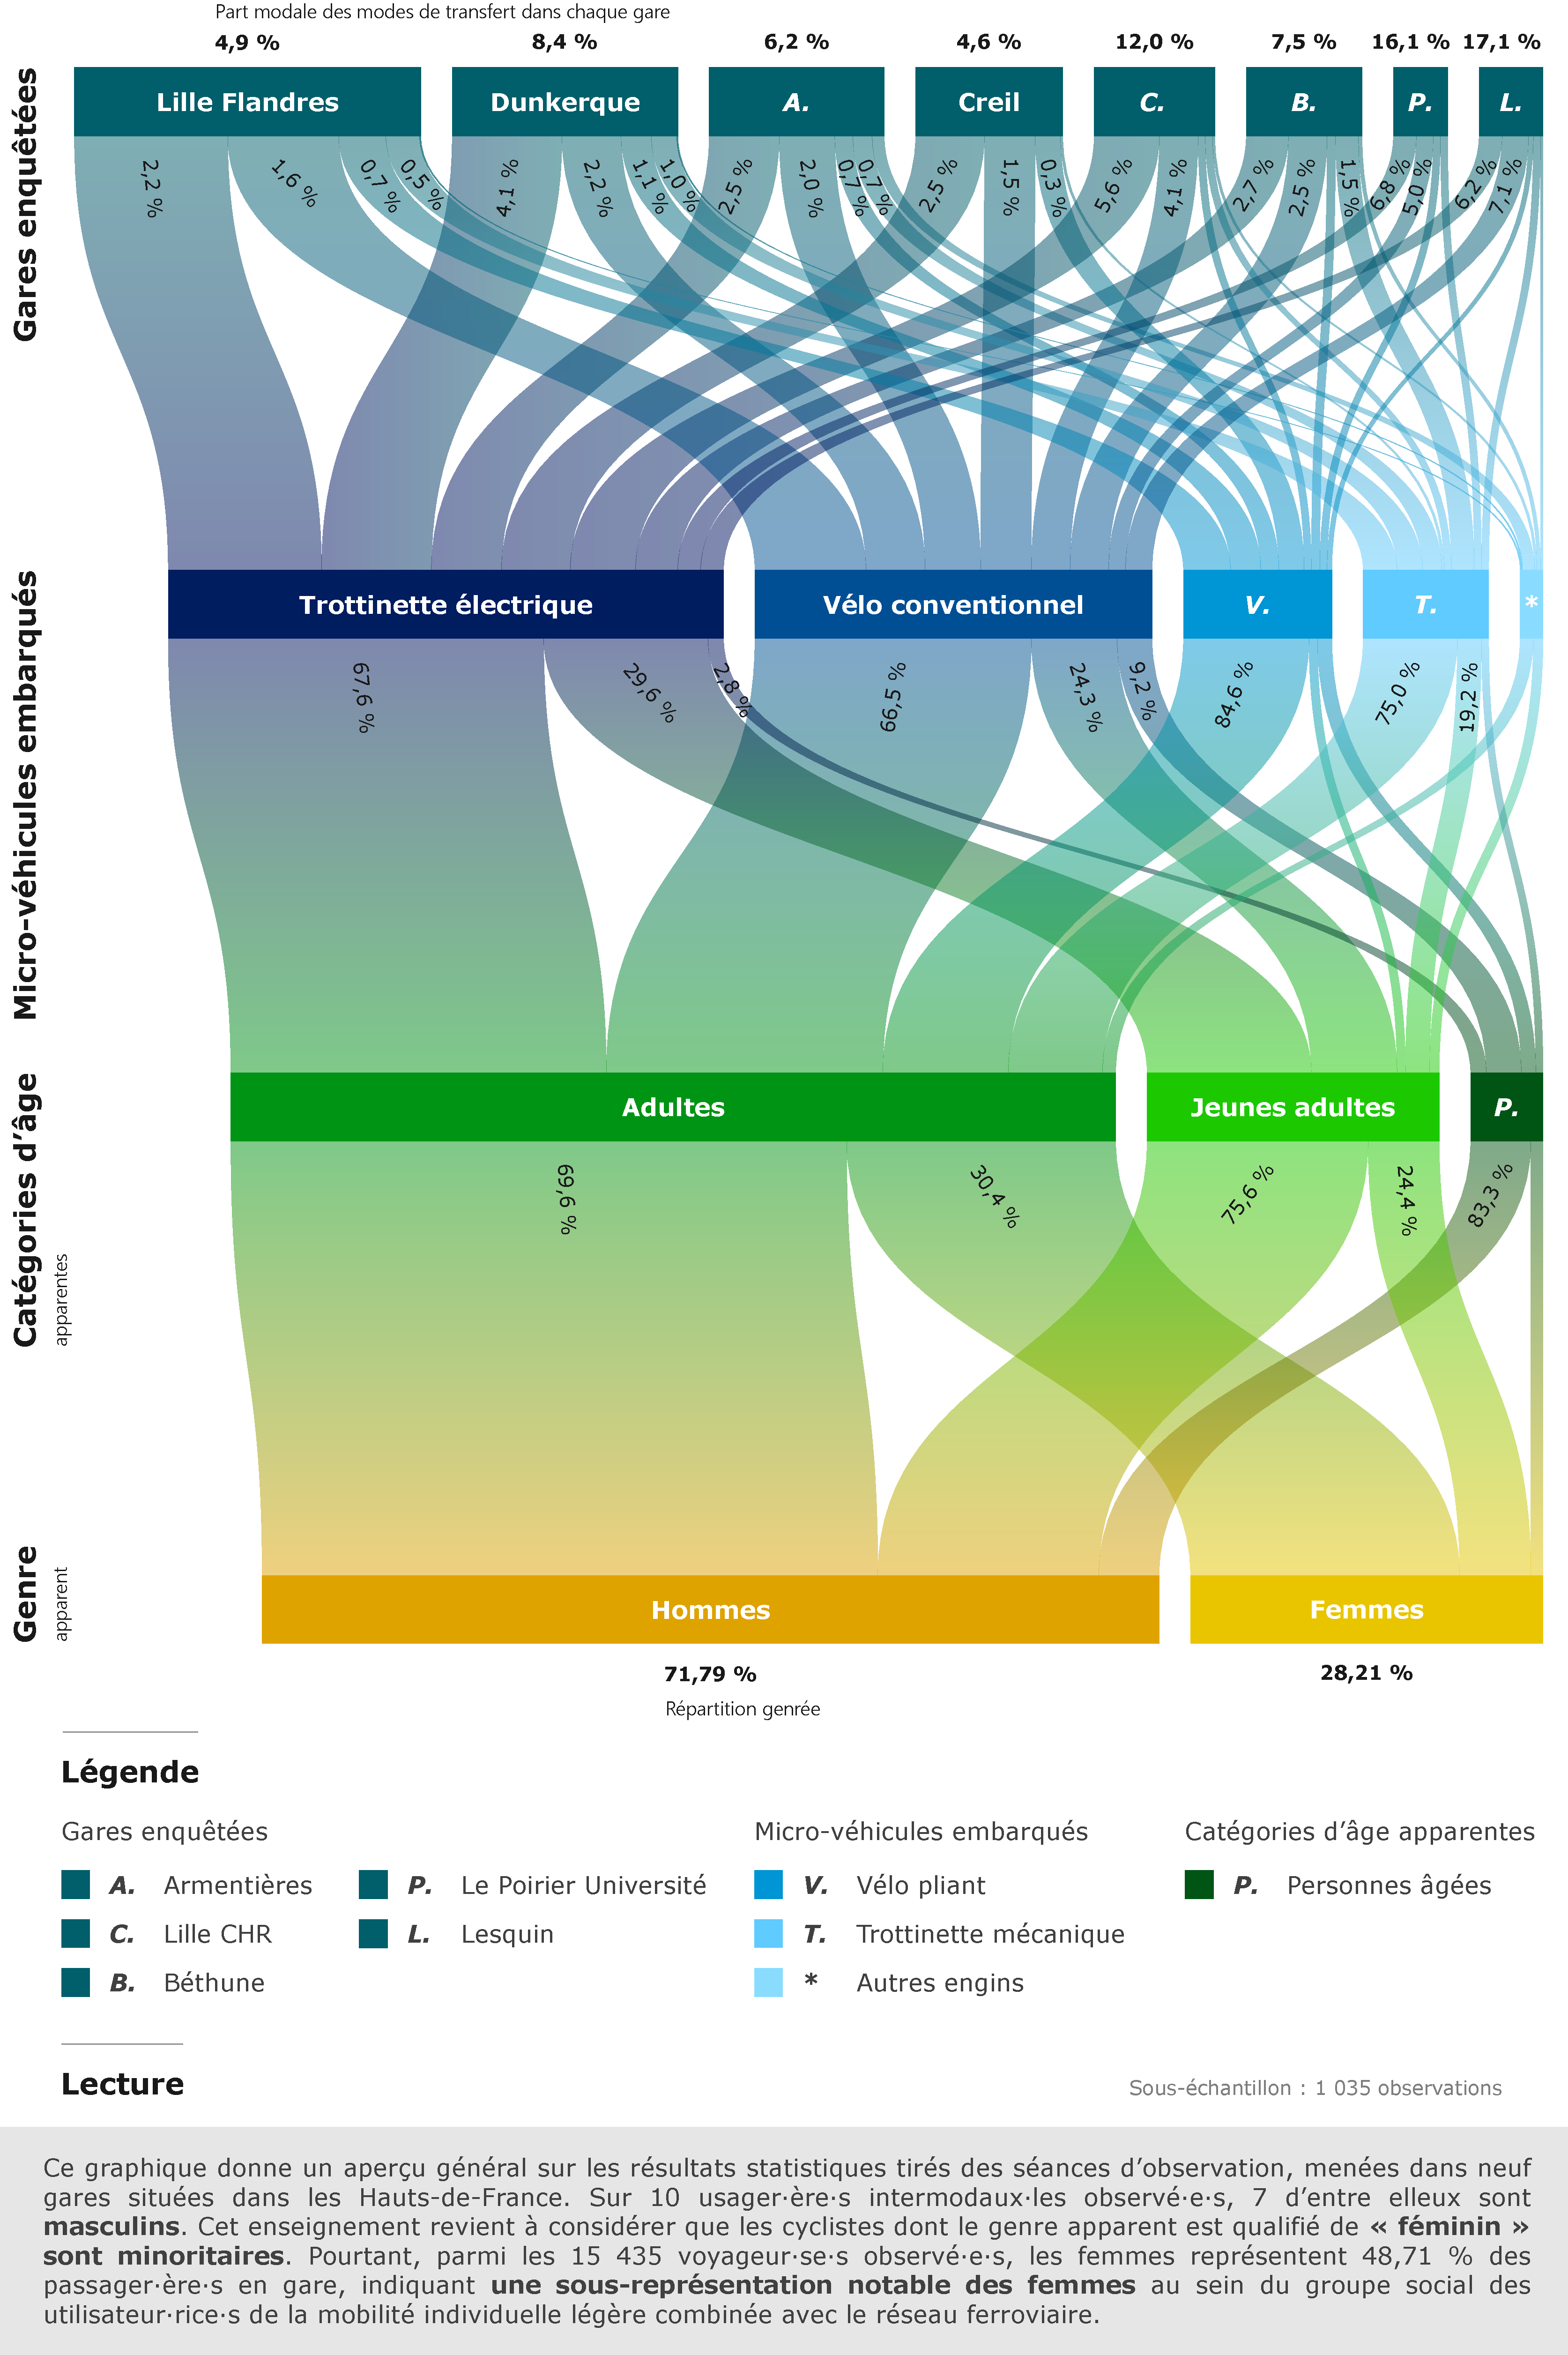
\includegraphics[width=1\columnwidth]{src/Figures/Chap-4/FR_Genre_Age.pdf}}
        \vspace{5pt}
        \begin{flushright}\scriptsize{
        Auteur~: \textcolor{blue}{Dylan Moinse (2024)}
        }\end{flushright}
    \end{figure}

    % Questionnaire - général et modes
Le questionnaire, dont la représentativité des résultats est limitée~–~cette technique repose sur la participation volontaire des répondant·e·s, ce qui peut introduire un biais de sélection~–~indique que 43~\% des cyclo-voyageur·se·s sont des femmes (90 réponses). Cette proportion varie de 40~\% à 47~\% pour le monoroue, le \textsl{skateboard}, le vélo pliant, la trottinette mécanique, le vélo classique et la mobilité partagée (avec respectivement 2, 10, 4, 47 et 7 réponses). La parité est même dépassée pour le \acrshort{VAE}, où les utilisatrices représentent 69~\% des participant·e·s (9 réponses). \textsl{A contrario}, la \acrshort{TEP} montre un déséquilibre considérable, avec seulement 28~\% de réponses féminines (11 réponses).%%Rédigé%%

    % Observation - croisée avec âge
En explorant conjointement les variables de genre et d'âge, l'analyse semble indiquer une accentuation des inégalités de genre avec l'avancement de l'âge, sans qu'il soit possible de déterminer si cela relève d'un effet d'âge ou d'un effet générationnel\footnote{
        D'une part, l'effet d'âge désigne les pratiques et les préférences qui se modifient naturellement et socialement avec l'âge de l'individu, indépendamment de sa génération. Ainsi, il est possible que les femmes plus jeunes montrent une préférence plus prononcée pour l'usage intermodal de la mobilité individuelle légère, ou que les hommes maintiennent plus longtemps ces modes de déplacement par rapport aux femmes, toutes choses étant égales par ailleurs. D'autre part, l'effet générationnel, ou effet de cohorte, se réfère aux attitudes et aux valeurs partagées par les individus d'une même génération. En ce sens, les femmes issues des générations Alpha et Z (entre 1997 et aujourd'hui) pourraient être davantage disposées à utiliser ces véhicules que celles issues de générations antérieures.
}. Selon les catégories d'âge établies, le déséquilibre en faveur des voyageurs masculins utilisant une \acrshort{TEP} se renforce progressivement : le ratio entre hommes et femmes est de 2,7 chez les \Guillemets{jeunes adultes}, passe à 3,1 chez les \Guillemets{adultes}, et atteint 12 chez les \Guillemets{personnes âgées}.%%Rédigé%%

    % Littérature - vélo
En écho aux recherches antérieures, ces statistiques descriptives s'alignent sur le corpus, certes limité, de la littérature scientifique portant sur la relation entre l'utilisation du vélo et le genre en France \textcolor{blue}{\autocite[1]{gaudron-arlon_gender_2022}}\index{Gaudron-Arlon, Léa|pagebf}. Pour l'ensemble des tranches d'âge, les hommes pratiquent le vélo près de trois fois plus fréquemment que les femmes, tandis que les femmes ont tendance à marcher davantage que les hommes \textcolor{blue}{\autocite[2]{rossignol_femmes_2023}}\index{Rossignol, Françoise|pagebf}\index{Faucheux, Valérie|pagebf}\index{Revel-Fourcade, Armelle|pagebf}\index{Delli, Karima|pagebf}. Dans le contexte de l'usage du vélo tant personnel que partagé, une analyse menée par \textcolor{blue}{Matthieu} \textcolor{blue}{\textcite{adam_quart_2018}}\index{Adam, Matthieu|pagebf} sur les dénombrements manuels réalisés par la Métropole de Lyon souligne la nette prédominance des cyclistes masculins, qui représentent 59~\% du total. Le rapport publié par \textcolor{blue}{\textcite[27]{6t-bureau_de_recherche_etude_2018}}\index{Bureau de recherche 6t@\textsl{Bureau de recherche 6t}|pagebf} se concentrant sur le profil des utilisateur·rice·s du \acrshort{VFF} à Paris corrobore ce constat général, avec une part de 68~\% d'hommes. La typologie des usager·ère·s du \acrshort{VLS} lyonnais \textsl{Vélo'v}, réalisée par \textcolor{blue}{\textcite[289]{vogel_bicycle_2014}}\index{Vogel, Marie|pagebf}\index{Hamon, Ronan|pagebf}\index{Lozenguez, Guillaume|pagebf}\index{Merchez, Luc|pagebf}\index{Abry, Patrice|pagebf}\index{Barnier, Julien|pagebf}\index{Borgnat, Pierre|pagebf}\index{Flandrin, Patrick|pagebf}\index{Mallon, Isabelle|pagebf}\index{Robardet, Céline|pagebf}, dévoile une répartition genrée inégale qui varie selon quatre catégories identifiées~: les \Guillemets{utilisateur·rice·s régulier·ère·s} et les \Guillemets{utilisateur·rice·s assidu·e·s} sont principalement masculins, alors que les catégories relatives aux \Guillemets{utilisateur·rice·s multimodaux·les} et aux \Guillemets{utilisateur·rice·s occasionnel·le·s} présentent une répartition genrée plus équilibrée. Dans le cadre de notre enquête, la distribution genrée de la mobilité individuelle légère associée au réseau ferroviaire n'a cependant pas de lien apparent avec la fréquence d'usage de ces combinaisons modales.%%Rédigé%%

    % Littérature - trottinette
Un schéma similaire émerge dans le contexte de l'essor récent de la \acrshort{TEP}, les hommes représentant plus ou moins 60~\% des utilisateur·rice·s de cet \acrshort{EDP} en France, comme en atteste l'étude de \textcolor{blue}{Cyprien} \textcolor{blue}{\textcite{richer_dossier_2021}}\index{Richer, Cyprien|pagebf} qui consolide environ 40 enquêtes de mobilité certifiées par le \acrfull{Cerema}. La prévalence des utilisateurs masculins, oscillant entre 68~\% et 75~\%, se retrouve également dans le marché de la \acrshort{TEFF}. Ces inégalités de genre dans la mobilité émergente se vérifient non seulement à Paris \textcolor{blue}{\autocites[46]{apur_mobilites_2020}[14]{6t-bureau_de_recherche_comprendre_2019}[annexes]{bortoli_consequential_2020}}\index{Bureau de recherche 6t@\textsl{Bureau de recherche 6t}|pagebf}\index{Apur@\textsl{Apur}|pagebf}\index{Bortoli, Anne de|pagebf}\index{Christoforou, Zoi|pagebf}, mais également à Lyon et à Marseille \textcolor{blue}{\autocite[50]{6t-bureau_de_recherche_usages_2019}}\index{Bureau de recherche 6t@\textsl{Bureau de recherche 6t}|pagebf}. De manière similaire au vélo, il a été constaté que les utilisateur·rice·s les plus fréquent·e·s des services de trottinette électrique sont majoritairement des hommes (68~\%) par rapport aux utilisateur·rice·s occasionnel·le·s (58~\%) dans ces trois métropoles françaises \textcolor{blue}{\autocite[65]{6t-bureau_de_recherche_usages_2019}}\index{Bureau de recherche 6t@\textsl{Bureau de recherche 6t}|pagebf}. Dans le contexte du réseau ferré en région Provence-Alpes-Côte d'Azur, nous avons identifié une part modale du vélo et de la \acrshort{TEP} largement appropriée par les hommes, avec des parts respectives de 79~\% et de 83~\%, alors que la répartition de l'ensemble des voyageur·se·s ferroviaires est paritaire et que celleux se connectant aux gares en voiture sont essentiellement des femmes \textcolor{blue}{\autocite[183]{moinse_intermodal_2022}}\index{Moinse, Dylan|pagebf}\index{Goudeau, Matthieu|pagebf}\index{L'Hostis, Alain|pagebf}\index{Leysens, Thomas|pagebf}.%%Rédigé%%

    % Conclusion
Cette analyse a permis de définir le profil socio-économique et démographique des usager·ère·s intermodaux·les utilisant la mobilité individuelle légère, de manière interroger ces synergies modales comme vecteurs de déséquilibres en matière de répartition par âge et par genre. Au sein de cette sous-section, axée sur les catégories d'âge et de genre, apparentes et déclarées par les voyageur·se·s, trois tendances principales se dégagent~: (i) la retranscription statistique d'une pratique de mobilité majoritairement investie par les adultes et (ii) par les hommes, tandis que (iii) la répartition genrée ne cesse d'être plus inégalitaire à mesure que l'âge des utilisateur·rice·s croît. Ainsi, l'association du vélo et de la micro-mobilité avec les systèmes de transport en commun n'est pas l'apanage des plus jeunes et se révèle nettement genrée.%%Rédigé%%

    % Transition
À l'heure où la mobilité individuelle légère, notamment les véhicules et services récemment intégrés à l'écosystème de la mobilité, est majoritairement adoptée par des usagers masculins, notre recherche empirique a pu souligner que la pratique intermodale de ces véhicules, marquée par une surreprésentation des hommes, ne déroge pas à la règle. L'usage de la trottinette motorisée, souvent favorisé en combinaison avec le train, représente ainsi un phénomène socio-culturel nouveau en ce sens que l'\acrshort{EDPM} est un objet de conception genrée, tout comme le vélo \textcolor{blue}{\autocites[16]{clewlow_micro-mobility_2018}[17]{sayagh_adolescentes_2018}[2]{abord_dechatillon_velo_2021}}\index{Abord de Chatillon, Margot|pagebf}\index{Ortar, Nathalie|pagebf}\index{Sayagh, David|pagebf}\index{Sayagh, David|pagebf}\index{Clewlow, Regina|pagebf}. Néanmoins, une partie de la documentation suggère que le profil des cyclistes tend à se diversifier lorsque la pratique du vélo est développée au sein des territoires. Plus un territoire est fréquenté par des cyclistes ou plus il est cyclable, plus le nombre de femmes utilisant le vélo augmenterait \textcolor{blue}{\autocite{lardellier_cadres_2021}}\index{Lardellier, Rémi|pagebf}. Cette hypothèse nous invite à nous interroger sur les moyens d'ouvrir la voie à des pratiques intermodales plus inclusives, en envisageant notamment l'amélioration de la cyclabilité comme levier potentiel. Nous avons l'intention d'approfondir cette hypothèse en interrogeant le rôle des facteurs liés à la pratique du vélo, à l'environnement urbain et à la qualité perçue des espaces publics sur la répartition genrée de ces pratiques de mobilité.%%Rédigé%%

    % ___________________________________________
    % 4.3.
    \newpage
    \needspace{1\baselineskip} % Réserve de l'espace
    \sectionheader{Inégalités de genre, urbanisme comme levier d'action}
\section{Disparités dans les pratiques de mobilité des cyclo-voyageur·se·s et le rôle modérateur de l’action par l’urbanisme
    \label{section-chap4:cyclabilite-genre}
    }

    %% Introduction
À partir d'une littérature scientifique récente consacrée aux liens complexes entre le vélo et le genre, la présente section vise à explorer les interrelations entre la part modale du vélo, l'environnement urbain favorable à la pratique du vélo et la participation féminine à ce mode de déplacement, dans le cadre d'une démarche empirique et comparative. En accord avec les recommandations formulées par \textcolor{blue}{\textcite[78]{goel_cycling_2022}}\index{Goel, Rahul|pagebf}\index{Goodman, Anna|pagebf}\index{Aldred, Rachel|pagebf}\index{Nakamura, Ryota|pagebf}\index{Tatah, Lambed|pagebf}\index{Garcia, Leandro Martin Totaro|pagebf}\index{Zapata-Diomedi, Belen|pagebf}\index{Sa, Thiago Herick de|pagebf}\index{Tiwari, Geetam|pagebf}\index{Nazelles, Audrey de|pagebf}\index{Tainio, Marko|pagebf}\index{Buehler, Ralph|pagebf}\index{Götschi, Thomas|pagebf}\index{Woodcock, James|pagebf}, cette recherche veille à examiner les multiples paramètres qui sous-tendent ces trois variables, en interrogeant le rôle des aménagements dans les territoires. Faut-il toutefois préciser que cette investigation s'efforce de dépasser le regard réducteur de la seule présence géographique d'itinéraires cyclables comme explication des problématiques relatives à la mobilité et au genre. Pour y parvenir, nous avons fait le choix d'embrasser la notion de \Guillemets{cyclabilité} en privilégiant les perceptions et l'expérience des cyclistes quant à la qualité de l'environnement urbain qu'iels fréquentent, en réponse aux principaux obstacles individuels entravant la pratique féminine de la mobilité individuelle légère.%%Rédigé%%

    %% Définition cyclabilité
De la même manière que la \gls{marchabilité} est liée à la marche, la \Guillemets{cyclabilité} se rapporte au degré de convivialité d'un territoire lié à la pratique du vélo, en favorisant à la fois la sécurité, la connectivité, le confort et le plaisir de se déplacer à vélo. L'évaluation de la cyclabilité s'exprime sous la forme d'une analyse du niveau de service offert aux cyclistes, que cela soit sous une perspective objective ou subjective, en prenant en considération des composantes telles que l'accessibilité \textcolor{blue}{\autocite[43]{lowry_assessment_2012}}\index{Lowry, Michael~B.|pagebf}\index{Callister, Daniel|pagebf}\index{Gresham, Maureen|pagebf}\index{Moore, Brandon|pagebf}. Malgré son rôle prépondérant, et pour partie en raison de la difficulté de sa mesure, l'appréciation subjective de la cyclabilité est souvent négligée, ce qui conduit à reléguer l'influence d'éléments critiques comme la sécurité, le confort et l'attractivité liés à l'usage du vélo \textcolor{blue}{\autocite[173]{gan_associations_2021}}\index{Gan, Zuoxian|pagebf}\index{Yang, Min|pagebf}\index{Zeng, Qingcheng|pagebf}\index{Timmermans, Harry~J.~P.|pagebf}.  La mesure de la cyclabilité peut être entreprise à diverses échelles, notamment à travers l'évaluation d'itinéraires cyclables spécifiques \textcolor{blue}{\autocites[5]{hardinghaus_more_2021}[44]{lowry_assessment_2012}[454]{krenn_development_2015}[55]{mcneil_bikeability_2011}[5]{wysling_where_2022}[6]{schmid-querg_munich_2021}}\index{Hardinghaus, Michael|pagebf}\index{Nieland, Simon|pagebf}\index{Lehne, Marius|pagebf}\index{Weschke, Jan|pagebf}\index{Lowry, Michael~B.|pagebf}\index{Callister, Daniel|pagebf}\index{Gresham, Maureen|pagebf}\index{Moore, Brandon|pagebf}\index{Krenn, Patricia Jasmin|pagebf}\index{Oja, Pekka|pagebf}\index{Titze, Sylvia|pagebf}\index{McNeil, Nathan|pagebf}\index{Wysling, Laura|pagebf}\index{Purves, Ross~S.|pagebf}\index{Schmid-Querg, Jonas|pagebf}\index{Keler, Andreas|pagebf}\index{Grigoropoulos, Georgios|pagebf} ou à un niveau géographique supérieur \textcolor{blue}{\autocites[4]{winters_bike_2016}[68]{gu_using_2018}[38]{nielsen_bikeability_2018}}\index{Winters, Meghan|pagebf}\index{Teschke, Kay|pagebf}\index{Brauer, Michael|pagebf}\index{Fuller, Daniel|pagebf}\index{Gu, Peiqin|pagebf}\index{Han, Zhiyuan|pagebf}\index{Cao, Zhejing|pagebf}\index{Chen, Yulin|pagebf}\index{Jiang, Yang|pagebf}\index{Nielsen, Thomas Alexander Sick|pagebf}\index{Skov-Petersen, Hans|pagebf}.%%Rédigé%%

    % 4.3.1.
    \needspace{1\baselineskip} % Réserve de l'espace
\subsection{Mobilisation des variables démographiques intégrées dans les méthodes mixtes mises en œuvre
    \label{chap4:materiau-empirique-genre}
    }

    % Introduction
La présente sous-section détaille les diverses bases de données exploitées dans le cadre de l'élaboration d'un modèle de régression statistique. Cette analyse est conçue pour étudier l'influence de facteurs liés à l'environnement urbain, tant mesuré que perçu, sur les pratiques différenciées du vélo et de la micro-mobilité selon le genre. Les variables dépendantes identifiées englobent le taux de participation féminine à l'usage exclusif du vélo ainsi que l'utilisation genrée de la mobilité individuelle légère en contexte intermodal. Les variables indépendantes, pour leur part, comprennent des éléments tels que la part modale du vélo, la densité de population, le réseau cyclable ainsi que le score de cyclabilité tel qu'il est perçu par les usager·ère·s. Cette structuration des données sous-jacente au modèle vise à dégager des perspectives pertinentes sur les dynamiques de genre dans l'espace urbain.%%Rédigé%%

    % Définition cyclabilité
Dans ce contexte, le cadre construit par les indicateurs indépendants se concentre sur plusieurs dimensions~: la part modale du vélo, la densité de population, la cyclabilité objective et la cyclabilité perçue. Pour ces deux dernières dimensions, nous intégrons des aspects liés à l'environnement urbain dans la cyclabilité mesurée, notamment la proportion des infrastructures cyclables et la proportion de zones~30 par rapport au réseau routier de chaque commune. La cyclabilité individuelle et perçue, en revanche, est évaluée à des niveaux agrégés pour chaque commune, sur la base des réponses collectées à partir du questionnaire analysé, qui englobe 5 dimensions et 26 questions thématiques sous-jacentes, allant de \(Q_{14}\) à \(Q_{39}\) (voir l'\hyperref[annexes:structure-questionnaire-fub-questions]{annexe~\ref{annexes:structure-questionnaire-fub-questions}}, page~\pageref{annexes:structure-questionnaire-fub-questions}). Cette méthode nous permet de proposer une analyse qui repose sur le système de mobilité (utilisation de la mobilité individuelle légère), le système urbain (densité de population), l'aménagement des espaces publics (infrastructure cyclable) et l'expérience individuelle des modes de déplacement dans les villes étudiées.%%Rédigé%%

    % 4.3.1.1.
    \needspace{1\baselineskip} % Réserve de l'espace
\subsubsection*{Analyse secondaire du fichier \textsl{MOBPro} issu du recensement de la population
    \label{source-mobpro}
    }

    %% \textsl{MOBPro} 2019 Description 1
La présente recherche empirique s'appuie, tout d'abord, sur les données du recensement périodique de la population française datant de 2019, réalisé par l'\textcolor{blue}{\textcite{insee_documentation_2023}}\index{Insee@\textsl{Insee}|pagebf}, et mené de manière quadriennale. Plus précisément, les données examinées découlent du fichier intitulé \Guillemets{\textsl{Mobilités Professionnelles}} (\textsl{MOBPro}), se consacrant exclusivement à l'étude des déplacements quotidiens réalisés par les individus vivant en France. Il convient de noter que pour répondre à ce questionnaire, les ménages avaient la possibilité de s'exprimer de manière individuelle, que ce soit par voie électronique ou postale. La base de données issue de ce recensement présente une représentativité précise des déplacements effectués entre le domicile et le lieu de travail, à partir d'un échantillon exhaustif englobant les personnes actives âgées de plus de 15 ans, résidant tant en France métropolitaine que dans les \acrfull{DROM-COM}\footnote{
    Les \acrfull{DROM} ont à la fois le statut de département et de région, et sont intégrés à la République française au même titre que les régions métropolitaines mentionnées précédemment. Les \acrshort{DROM} font partie des territoires ultramarins français \acrshort{DROM-COM}, avec les \acrfull{COM} qui disposent d'un statut différent ainsi que d'une plus grande autonomie vis-à-vis de la France métropolitaine.
}, mis à part Mayotte.%%Rédigé%%

    %% \textsl{MOBPro} 2019 Description 2
Les questions formulées et mobilisées au sein du jeu de données \textsl{MOBPro} portent essentiellement sur deux variables, à savoir les lieux de travail au niveau communal (\(Q^{Insee}_{20}\)) et le principal mode de déplacement (\(Q^{Insee}_{22}\)). Chaque individu est anonymisé et fait l'objet d'une description de ses déplacements pendulaires, de ses caractéristiques socio-démographiques, ainsi que des localisations résidentielles et professionnelles à l'échelle communale. La prise en compte des facteurs de pondération spécifiques à chaque individu permet d'employer ces données pour constituer un échantillon représentatif, lorsqu'il existe au moins 200 réponses par commune \textcolor{blue}{\autocite{insee_documentation_2023}}\index{Insee@\textsl{Insee}|pagebf}. En outre, il convient de signaler une modification apportée au questionnaire à partir de 2015, qui s'est traduite par une distinction nette entre le \Guillemets{vélo} et les \Guillemets{véhicules motorisés à deux roues} \textcolor{blue}{\autocite{razemon_pour_2013}}\index{Razemon, Olivier|pagebf}. Cette modification a été implémentée dans la question~\(Q^{Insee}_{22}\), qui inclut désormais explicitement les \Guillemets{vélos (y compris les vélos à assistance électrique)}.%%Rédigé%%

    %% \textsl{MOBPro} 2019 Echantillonnage 1
La base de données \textsl{MOBPro} de 2019, englobant un contingent global de 7~932~895 individus, contient un ensemble de variables filtrées, dont notamment le poids individuel (\Guillemets{\(IPONDI\)}), le mode de déplacement principalement emprunté pour les déplacements domicile-travail (\Guillemets{\(TRANS\)}), le lieu de résidence (\Guillemets{\(COMMUNE\)}), et le genre (\Guillemets{\(SEXE\)}). La première condition d'inclusion, appliquée au moyen d'une série de codes \textsl{Python}, se concentre sur le mode de déplacement principal associé au vélo (\Guillemets{\(TRANS~=~3\)}), excluant par conséquent les autres modalités de mobilité, telle que réalisée par \textcolor{blue}{\textcite[7]{raux_does_2021}}\index{Raux, Charles|pagebf}\index{Lamatkhanova, Ayana|pagebf}\index{Grassot, Lény|pagebf}. Cette démarche exclut les déplacements intermodaux où le vélo intervient comme mode de déplacement secondaire, en raison des paramètres statistiques appliqués\footnote{
    Dans la plupart des enquêtes sur la mobilité en France, la hiérarchisation des modes de déplacement est généralement établie en fonction du mode principal employé pour les déplacements intermodaux. Les \textsl{Enquêtes Mobilité Certifiées \acrshort{Cerema}} se conforment à la convention établie par le \textcolor{blue}{\textcite[32]{cerema_enquetes_2020}} qui accorde la primauté aux modes dits \Guillemets{structurants}.
} \textcolor{blue}{\autocite[32]{cerema_enquetes_2020}}. Cette procédure a donné naissance à un sous-échantillon regroupant 409~326 individus, composé de 253~464 cyclistes masculins et 155~862 cyclistes féminines. L'analyse statistique descriptive met en évidence que seulement 1,5~\% des femmes ont déclaré utiliser le vélo pour leurs déplacements domicile-travail, en contraste avec 3,7~\% des hommes.%%Rédigé%%

    %% \textsl{MOBPro} 2019 Echantillonnage 2
La seconde phase d'exclusion appliquée à la base de données \textsl{MOBPro} a consisté en l'agrégation des navetteur·se·s au sein de communes similaires \textcolor{blue}{\autocite{insee_documentation_2023}}\index{Insee@\textsl{Insee}|pagebf}, suivant la démarche entreprise par \textcolor{blue}{\textcite[259]{papaix_potential_2022}}\index{Papaix, Claire|pagebf}\index{Dupont-Kieffer, Ariane|pagebf}\index{Palmier, Patrick|pagebf}. Les réponses ayant été regroupées et n'ayant pas atteint le seuil de signifiance, soit 200 cyclistes, ont été exclues, dans le but de maintenir une diversité représentative de territoires\footnote{
    Dans la documentation de l'\textcolor{blue}{\textcite{insee_documentation_2023}}, à propos du fichier \Guillemets{MOBPro}, les \Guillemets{\Guillemets{effectifs supérieurs à 500 peuvent normalement être utilisés en toute confiance. Les effectifs inférieurs à 200 doivent être maniés avec précaution car, en raison de l'imprécision liée au sondage, ils peuvent ne pas être significatifs. De ce fait, les comparaisons entre territoires de petite taille sont à proscrire. Pour des zones de moins de 2~000 habitants, il est recommandé de ne pas utiliser les données issues de l'exploitation complémentaire.}}.
}. À la suite de la mise en œuvre de ce filtre sélectif, parmi les 10~520 communes comptant au moins un individu pratiquant le vélo dans la base de données, 144 municipalités ont été retenues, comprenant 128~492 cyclistes, dont 76~773 hommes et 51~719 femmes. Parmi les 144 communes sélectionnées, 65 d'entre elles sont des villes centres, tandis que les 79 autres relèvent de communes périphériques.%%Rédigé%%

    % 4.3.1.2.
   \needspace{1\baselineskip} % Réserve de l'espace
\subsubsection*{Mobilisation de l’observation quantitative
    \label{chap4:variables-age-genre-observation-quantitative}
    }

    %% Justification Observation Quantitative
Outre l'analyse secondaire des bases de données mentionnées, la présente recherche empirique s'appuie sur la mise en œuvre de l'observation quantitative en vue de saisir les profils démographiques des usager·ère·s de la micro-mobilité au sein de notre étude de cas, centrée sur la région Hauts-de-France. Du fait que ces données secondaires se limitent à l'usage du vélo, il nous paraît essentiel d'intégrer les modes de déplacement associés à la micro-mobilité émergente, tels que la \acrshort{TEP}. Cette méthode de collecte de données vise également à obtenir un échantillon représentatif des voyageur·se·s intermodaux·les combinant ainsi la mobilité individuelle légère avec les réseaux de transport en commun.%%Rédigé%%

    % 4.3.1.3.
    \needspace{1\baselineskip} % Réserve de l'espace
\subsubsection*{Exploitation du \textsl{Baromètre des Villes Cyclables}
    \label{chap4:source-barometre-fub}
    }

    %% FUB Baromètre Description
La seconde source de données mobilisée en vue de collecter cette fois-ci les attributs liés à l'environnement cyclable repose sur l'exploitation du questionnaire biannuel du \Guillemets{\textsl{Baromètre des Villes Cyclables}} de 2021, élaboré par la \textcolor{blue}{\textcite{fub_barometre_2021}}\index{FUB@\textsl{FUB}|pagebf} en France. En cours de déploiement depuis 2017, ce baromètre se propose d'évaluer la cyclabilité des communes françaises, à travers la compilation des retours d'expérience des cyclistes concernant aussi bien la qualité des infrastructures cyclables, des politiques cyclables mises en œuvre, que l'expérience globale des usager·ère·s. L'objectif de ce questionnaire en ligne consiste à appréhender la \gls{perception} générale qu'ont les utilisateur·rice·s du vélo en France, et à opérer un classement des communes en fonction de leur degré de convivialité perçue à l'égard du vélo. Aujourd'hui, ce baromètre jouit d'une position de référence pour les autorités locales, les associations, la recherche et la population. Cette sous-partie dédiée à l'étude du genre dans la mobilité intègre ainsi dans son analyse la notion de \Guillemets{cyclabilité subjective}, reconnaissant ainsi que la sécurité est une dimension aussi bien collective qu'individuelle, façonnée par l'expérience des cyclistes \textcolor{blue}{\autocite[57]{garrard_promoting_2008}}\index{Garrard, Jan|pagebf}\index{Rose, Geoffrey|pagebf}\index{Lo, Sing Kai|pagebf}\index{Rose, Geoffrey|pagebf}\index{Lo, Sing Kai|pagebf}. De plus, conformément aux observations de \textcolor{blue}{\textcite[303]{ma_peoples_2017}}\index{Ma, Liang|pagebf}\index{Dill, Jennifer|pagebf}, un décalage a été observé entre l'environnement objectif et l'environnement perçu en matière de convivialité pour le vélo, particulièrement en ce qui concerne son usage utilitaire et en partie attribué à la tolérance au risque qui varie en fonction du genre.%%Rédigé%%

    %% FUB Baromètre Questions
Le questionnaire se rapportant à la cyclabilité a été administré en ligne, offrant ainsi l'opportunité tant aux cyclistes qu'aux non-usager·ère·s d'évaluer leurs expériences ou leurs perceptions et de formuler leurs opinions à l'égard des conditions liées à la pratique du vélo. Les évaluations ont été conduites sur une échelle de notation allant de 1~–~exprimant un niveau de satisfaction \textsl{très insatisfaisant}~–~à 6~–~\textsl{très satisfaisant}. Les diverses évaluations émises par les participant·e·s ont été ensuite mises en confrontation pour donner lieu à une évaluation globale de la cyclabilité de chaque commune concernée (voir l'\hyperref[annexes:structure-questionnaire-fub-questions]{annexe~\ref{annexes:structure-questionnaire-fub-questions}}, page~\pageref{annexes:structure-questionnaire-fub-questions}). Ce questionnaire libre d'accès comprend un ensemble de vingt-six questions en relation avec les expériences de déplacement à vélo des répondant·e·s, organisées en cinq thèmes distincts~: (i) \Guillemets{ressenti global}, (ii) \Guillemets{sécurité}, (iii) \Guillemets{confort}, (iv) \Guillemets{efforts de la ville}~et (v) \Guillemets{services et stationnement}. À l'aide d'un score global, les communes se voient attribuer une position dans une échelle allant de~\(A+\) (notant un score supérieur à 4,6 sur~6) à~\(G\) (désignant un score inférieur à 2,3 sur 6), correspondant à une mention sur le \Guillemets{climat vélo} des territoires, allant de \Guillemets{conditions excellentes} à des \Guillemets{conditions très défavorables} \textcolor{blue}{\autocite{fub_barometre_2021}}\index{FUB@\textsl{FUB}|pagebf}. Il faut noter que la moyenne des scores obtenue par chaque commune française atteint un niveau de cyclabilité générale de 2,98 sur 6 \textcolor{blue}{\autocite[17]{vermeulen_barometre_2022}}\index{Vermeulen, Thibault|pagebf}\index{Kaouane, Carole|pagebf}. L'énoncé détaillé de chaque question faisant l'objet d'une notation dans le cadre de ce baromètre est présenté dans l'\hyperref[annexes:structure-questionnaire-fub-tableau]{annexe~\ref{annexes:structure-questionnaire-fub-tableau}} (page~\pageref{annexes:structure-questionnaire-fub-tableau}).%%Rédigé%%

    % Tableau Liste communes
% Tableau Liste communes
%%Rédigé%%
    \begin{table}[h!]
    \centering
    \renewcommand{\arraystretch}{1.5}
    \resizebox{\columnwidth}{!}{
    \begin{tabular}{p{0.34\columnwidth}p{0.56\columnwidth}p{0.1\columnwidth}}
        %\hline
    \rule{0pt}{15pt} \small{\textcolor{blue}{{\textbf{Région}}}} & \small{\textcolor{blue}{{\textbf{Villes centres}}}} & \small{\textcolor{blue}{{\textbf{Effectif}}}}\\
        \hline
\multirow{1.5}{*}{\small{Auvergne-Rhône-Alpes}} & \small{Annecy, Chambéry, Clermont-Ferrand, Grenoble, Lyon, Saint-Étienne et Valence} & \multirow{1.5}{*}{\small{7}}\\
\small{Bourgogne-Franche-Comté} & \small{Besançon et Dijon} & \small{2}\\
\small{Bretagne} & \small{Brest, Lorient, Rennes et Saint-Nazaire} & \small{4}\\
\small{Centre-Val de Loire} & \small{Orléans et Tours} & \small{2}\\
\multirow{1.5}{*}{\small{Grand Est}} & \small{Metz, Mulhouse, Nancy, Reims, Strasbourg et Troyes} & \multirow{1.5}{*}{\small{6}}\\
\multirow{1.5}{*}{\small{Hauts-de-France}} & \small{Amiens, Arras, Beauvais, Douai, Dunkerque, Lille et Valenciennes} & \multirow{1.5}{*}{\small{7}}\\
\small{Île-de-France} & \small{Paris} & \small{1}\\
\small{Normandie} & \small{Caen, Le Havre et Rouen} & \small{3}\\
\multirow{1.5}{*}{\small{Nouvelle-Aquitaine}} & \small{Angoulême, Bayonne, Bordeaux, La Rochelle, Limoges et Poitiers} & \multirow{1.5}{*}{\small{6}}\\
\small{Occitanie} & \small{Montpellier, Nîmes, Perpignan et Toulouse} & \small{4}\\
\small{Pays de la Loire} & \small{Angers, Le Mans et Nantes} & \small{3}\\
\multirow{1.5}{*}{\small{Provence-Alpes-Côte d'Azur}} & \small{Aix-en-Provence, Avignon, Marseille, Nice et Toulon} & \multirow{1.5}{*}{\small{5}}\\
\small{La Réunion} & \small{Saint-Denis, Saint-Paul et Saint-Pierre} & \small{3}\\
        \hline
        \end{tabular}}
    \caption{Liste des 53 communes françaises examinées dans le cadre de l'étude sur la cyclabilité mise en relation avec la pratique genrée du vélo et de la micro-mobilité.}
    \label{table-chap4:communes-fub-insee}
        \vspace{5pt}
        \begin{flushleft}\scriptsize
        \textcolor{blue}{Lecture~:} ce tableau recense les 53 communes françaises réparties dans 13 régions, incluant des métropoles et des villes moyennes, afin d'étudier les liens entre leur cyclabilité et la pratique genrée du vélo.
        \end{flushleft}
        \begin{flushright}\scriptsize{
        Jeux de données~: \textsl{MOBPro} \textcolor{blue}{\autocite{insee_documentation_2023}} et \textsl{Baromètre des Villes Cyclables} \textcolor{blue}{\autocite{fub_barometre_2021}}
        \\
        Auteur~: \textcolor{blue}{Dylan Moinse (2023)}
        }\end{flushright}
        \end{table}%%Rédigé%%

    %% FUB Baromètre Echantillonnage
L'enquête de la \textcolor{blue}{\textcite{fub_barometre_2021}}\index{FUB@\textsl{FUB}|pagebf} s'est déroulée sur une période allant du 14 septembre au 30 novembre 2021, ayant réuni un total de 277~384 réponses, parmi lesquelles 250~228 émanent de cyclistes. Seules les communes ayant bénéficié d'au moins 50 retours d'expérience de la part des cyclistes ont été retenues pour l'établissement du classement du baromètre. Ce sont dès lors 1~625 communes qui sont représentées à travers cette troisième édition, réparties en diverses catégories, à savoir~: 38 grandes villes, 218 villes de taille moyenne, 353 petites communes, 292 villages, 719 communes de banlieue et 5 îles \textcolor{blue}{\autocite[7]{vermeulen_barometre_2022}}\index{Vermeulen, Thibault|pagebf}\index{Kaouane, Carole|pagebf}. Parmi les cyclistes ayant pris part à l'enquête du \textsl{Baromètre des Villes Cyclables} de 2021, 46~\% d'entre elleux s'identifient comme des femmes, sans tenir compte des répondant·e·s n'ayant pas spécifié leur identité de genre. Ce taux de réponse reflète une augmentation de quatre points en faveur de la participation féminine par rapport à l'édition de 2019 \textcolor{blue}{\autocite[10]{vermeulen_barometre_2022}}\index{Vermeulen, Thibault|pagebf}\index{Kaouane, Carole|pagebf}. En procédant à une jointure attributaire entre les 144 villes recensant plus de 200 cyclistes ayant répondu à la base de données \textsl{MOBPro} et les villes positionnées dans le \textsl{Baromètre des Villes Cyclables} qui ont cumulé au moins 100 évaluations individuelles, le processus d'échantillonnage a conservé un effectif de 64 communes françaises. Par la suite, nous avons choisi de ne conserver que les villes centres des agglomérations françaises dans l'échantillon, aboutissant ainsi à un échantillon final de 53 villes. La liste de ces 53 communes, classées selon leurs régions respectives, est présentée dans le \hyperref[table-chap4:communes-fub-insee]{tableau \ref{table-chap4:communes-fub-insee}} (page~\pageref{table-chap4:communes-fub-insee}).%%Rédigé%%

    % 4.3.1.4.
    \needspace{1\baselineskip} % Réserve de l'espace
\subsubsection*{Sources de données cartographiques
    \label{chap4:source-cartographique}
    }

    %% OpenStreetMap
Au moyen de l'échantillonnage basé sur ces deux bases de données, nous avons été en mesure de caractériser les cinquante-trois agglomérations françaises, au sujet de la part modale et de l'usage genré du vélo, ainsi que de la cyclabilité subjective du territoire. Par la suite, dans le but de quantifier la dimension infrastructurelle, ces variables ont été sensiblement enrichies de données secondaires tirées d'\textcolor{blue}{\textcite{openstreetmap_openstreetmap_2023}}\index{OpenStreetMap@\textsl{OpenStreetMap}|pagebf} et extraites le 21 août~2023. Ces données cartographiques apportent un accès à des informations géographiques concernant l'infrastructure cyclable dans une ville donnée. De surcroît, cette recherche sur la mobilité et le genre a intégré des données issues de la \Guillemets{\textsl{Base nationale des aménagements cyclables}} créée par \textcolor{blue}{\textcite{velo__territoires_atlas_2023}}\index{Vélo \& Territoires@\textsl{Vélo \& Territoires}|pagebf} et de la \Guillemets{\textsl{Grille de densité municipale}} de l'\textcolor{blue}{\textcite{insee_grille_2021}}\index{Insee@\textsl{Insee}|pagebf}. L'apport de ces données cartographiques permet alors d'évaluer la cyclabilité objective de chaque commune à partir de la proportion d'aménagements cyclables dans le réseau viaire et de la densité de population dans les communes comparées.%%Rédigé%%

    % 4.3.2.
    \needspace{1\baselineskip} % Réserve de l'espace
\subsection{Élaboration d'un cadre d'analyse statistique
    \label{chap4:methodologie-modele-ols}
    }

    % Introduction
Le modèle de régression mis en œuvre dans cette section vise à interroger l'influence des facteurs sur l'usage du vélo et de la micro-mobilité, spécifique à chaque genre, tant dans les contextes monomodaux qu'intermodaux. Le \hyperref[fig-chap4:schema-methodologie-ols]{schéma~\ref{fig-chap4:schema-methodologie-ols}} (page~\pageref{fig-chap4:schema-methodologie-ols}) présente le cadre méthodologique utilisé pour mener à bien une \acrfull{OLS}, ou une régression des moindres carrés ordinaires, incluant les étapes préliminaires nécessaires à l'évaluation des hypothèses du modèle et à sa validation. Les étapes et les équations employées ont été détaillées dans l'\hyperref[annexes:methodologie-ols-etapes]{annexe~\ref{annexes:methodologie-ols-etapes}} (page~\pageref{annexes:methodologie-ols-etapes}).%%Rédigé%%

    %% Figure Schéma méthodologique OLS
    \begin{figure}[h!]\vspace*{4pt}
        \caption{Schéma du processus de modélisation des moindres carrés ordinaires examinant les interactions entre la cyclabilité et l'usage genré du vélo et de la micro-mobilité.}
        \label{fig-chap4:schema-methodologie-ols}
        \centerline{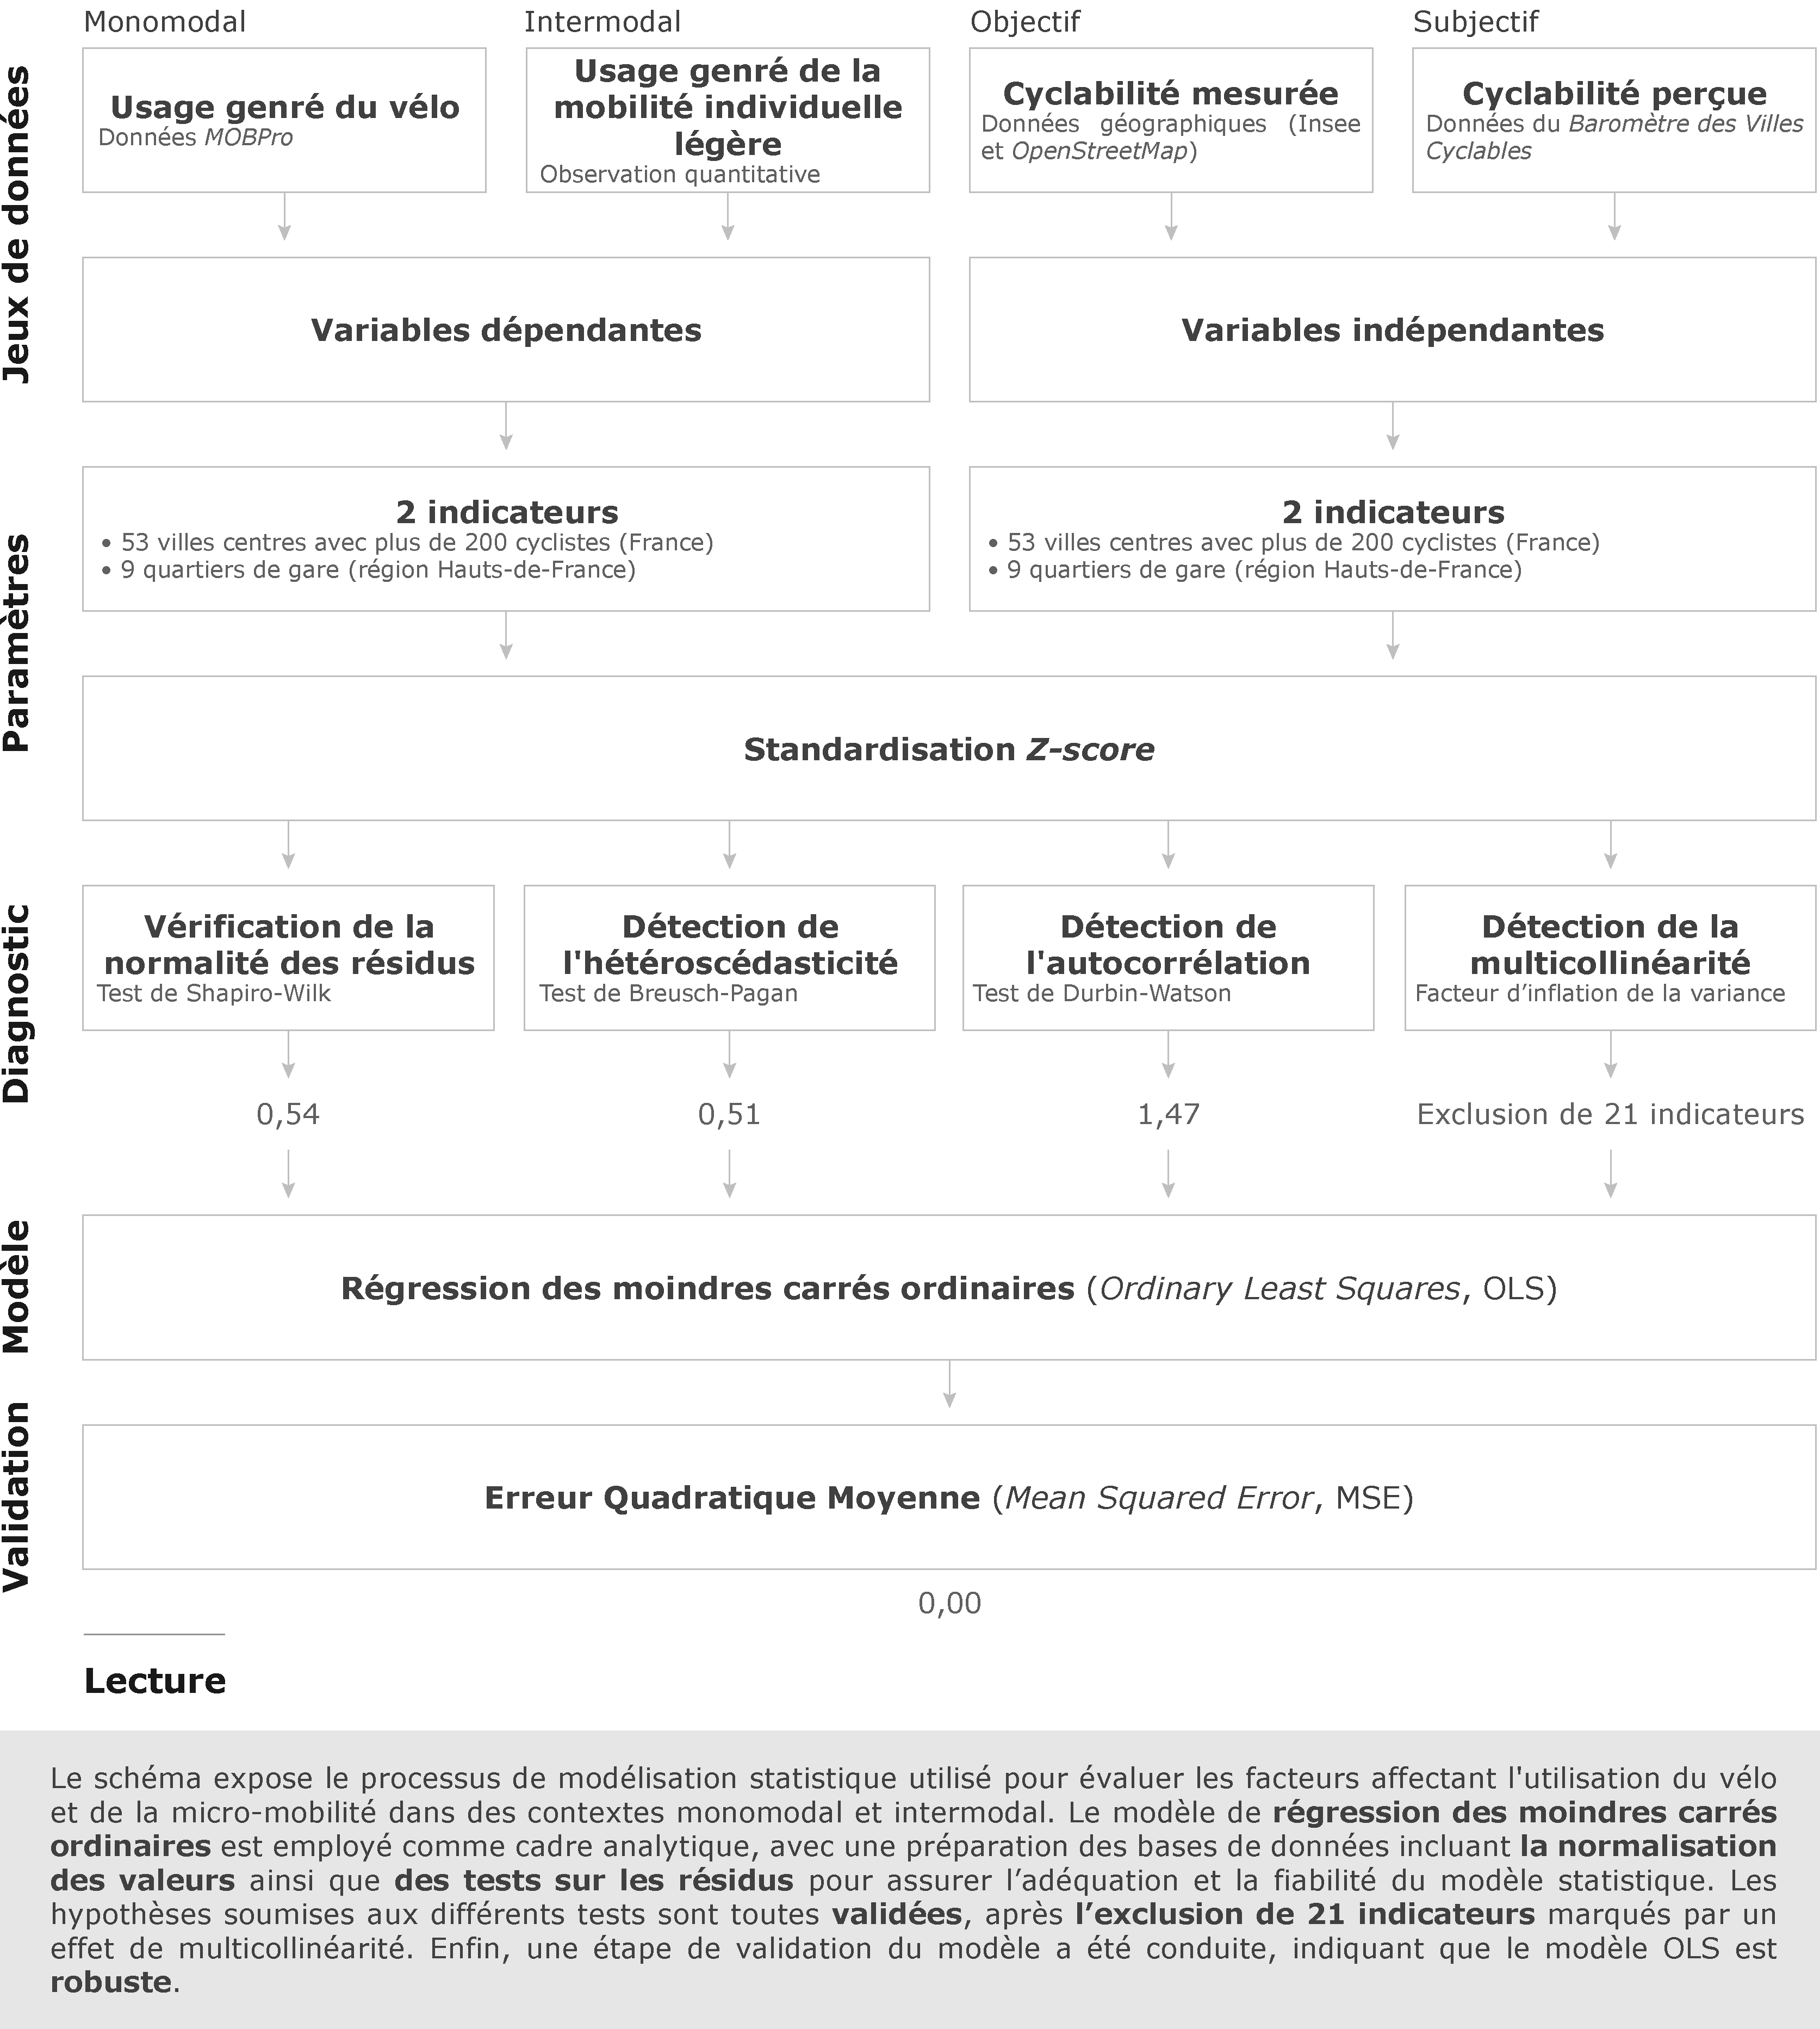
\includegraphics[width=1\columnwidth]{src/Figures/Chap-4/FR_Schema_Methodologie_OLS.pdf}}
        \vspace{5pt}
        \begin{flushright}\scriptsize{
        Auteur~: \textcolor{blue}{Dylan Moinse (2023)}
        }\end{flushright}
    \end{figure}

    % Modèle OLS
L'analyse secondaire se trouve adossée à deux bases de données sollicitées pour étayer notre démarche, à savoir la base de données \textsl{MOBPro} de 2019 \textcolor{blue}{\autocite{insee_documentation_2023}}\index{Insee@\textsl{Insee}|pagebf} et le \textsl{Baromètre des Villes Cyclables} de 2021 \textcolor{blue}{\autocite{fub_barometre_2021}}\index{FUB@\textsl{FUB}|pagebf}. Cette analyse s'appuie, en outre, sur l'observation quantitative émanant de notre étude de cas. Le recours à des méthodes statistiques descriptives conjugué au développement d'un modèle de régression linéaire constitue la démarche méthodologique employée dans cette sous-partie. Dans cette perspective, la régression \acrshort{OLS} a été choisie pour cette recherche en raison de sa robustesse pour estimer les relations linéaires entre une variable dépendante et plusieurs variables indépendantes. L'objectif principal de cette recherche est de clarifier la manière dont divers facteurs influencent la part modale des femmes utilisant le vélo dans différentes villes françaises. La régression \acrshort{OLS} est particulièrement appropriée à cet objectif, car elle permet d'obtenir des estimations non biaisées et efficaces des coefficients de régression, sous réserve que certaines hypothèses soient vérifiées. De plus, elle permet de quantifier l'impact de chaque variable explicative tout en contrôlant les effets des autres variables du modèle. En outre, la sélection d'une telle méthode statistique prend inspiration de recherches académiques antérieures ayant employé des techniques similaires pour explorer les relations entre les caractéristiques socio-démographiques d'une population et son environnement urbain. Le présent travail de recherche trouve ainsi son inspiration dans l'investigation menée par \textcolor{blue}{\textcite[64]{goel_cycling_2022}}\index{Goel, Rahul|pagebf}\index{Goodman, Anna|pagebf}\index{Aldred, Rachel|pagebf}\index{Nakamura, Ryota|pagebf}\index{Tatah, Lambed|pagebf}\index{Garcia, Leandro Martin Totaro|pagebf}\index{Zapata-Diomedi, Belen|pagebf}\index{Sa, Thiago Herick de|pagebf}\index{Tiwari, Geetam|pagebf}\index{Nazelles, Audrey de|pagebf}\index{Tainio, Marko|pagebf}\index{Buehler, Ralph|pagebf}\index{Götschi, Thomas|pagebf}\index{Woodcock, James|pagebf}, qui s'est servie de ces corrélations afin d'identifier les liens existants entre les caractéristiques socio-démographiques des cyclistes et l'environnement urbain, dans dix-sept pays distincts.%%Rédigé%%

    % Formule
Dans cette analyse statistique, la variable dépendante est la proportion de l'usage de la mobilité individuelle légère par les femmes, tandis que tous les autres indicateurs analysés servent de variables indépendantes. Ces indicateurs incluent la part modale globale du vélo, le taux d'infrastructures cyclables et des zones~30 en comparaison du réseau viaire, la densité de population ainsi que les sous-questions établissant le score de cyclabilité perçu tiré du questionnaire, totalisant l'intégration de 35 variables. L'analyse multivariée a été réalisée à l'aide de la régression \acrshort{OLS}, nous permettant d'évaluer l'effet combiné de toutes les variables indépendantes sur la variable dépendante. La \hyperref[equation:ols]{formule de régression~\ref{equation:ols}} (page~\pageref{equation:ols}) est mise en application pour estimer la relation linéaire entre les variables dépendantes et l'ensemble des variables indépendantes\footnote{
    Dans ce contexte, l'ordonnée à l'origine représente la valeur estimée de la variable dépendante \(Y\) (la part modale genrée du vélo) lorsque toutes les variables indépendantes \(X_i\) sont égales à zéro. Il s'agit du point où la ligne de régression estimée coupe l'axe des ordonnées. En d'autres termes, \(\hat{\beta}_0\) est la valeur de \(Y\) prévue par le modèle lorsque les contributions de toutes les variables indépendantes sont nulles. Cela donne une base de référence pour interpréter les effets des indicateurs indépendants sur la part modale genrée du vélo.
    } \textcolor{blue}{\autocite{strang_introduction_1986}}\index{Strang, Gilbert|pagebf}. La modélisation nécessite cependant de vérifier que les hypothèses de linéarité, d'indépendance, d'homoscédasticité et de normalité des erreurs soient respectées. L'étape suivante consiste dès lors à tester les hypothèses du modèle pour affiner et améliorer le modèle statistique.%%Rédigé%%

    % Équation OLS
\begin{equation}
\label{equation:ols}
\begin{aligned}
Y = \hat{\beta}_0 + \sum_{i=1}^{n} \hat{\beta}_i X_i + \epsilon
\end{aligned}
\end{equation}
\begin{align*}
    &\text{où~:} \\
    &Y \text{ représente la part modale genrée du vélo~;} \\
    &\hat{\beta}_0 \text{ est l'ordonnée à l'origine estimée~;} \\
    &\hat{\beta}_i \text{ est le coefficient estimé pour chaque variable indépendante}~i\text{~;}\\
    &X_i \text{ représente les variables indépendantes}~i\text{~;}\\
    &\epsilon \text{ est le terme d'erreur~;} \\
    &n \text{ est le nombre total d'indicateurs indépendants.}
\end{align*}%%Rédigé%%

    % 4.3.2.1.
    \needspace{1\baselineskip} % Réserve de l'espace
\subsubsection*{Vérification des hypothèses du modèle
    \label{chap4:methodologie-hypotheses}
    }

    % Z-score
La première étape dans le nettoyage de bases de données fusionnées consiste à normaliser les variables explicatives avant de procéder aux étapes spécifiques au modèle de régression. Lorsque les caractéristiques présentent différentes échelles, il peut être difficile de comparer directement les coefficients de régression. La standardisation place toutes les variables sur la même échelle, facilitant ainsi la comparaison des effets relatifs des variables explicatives. Avant l'entraînement du modèle, la distribution des données est ajustée pour avoir une moyenne de 0 et un écart-type de 1 grâce à la normalisation par le score~\(Z\). Cette méthode, couramment utilisée en régression linéaire \textcolor{blue}{\autocite{pearson_lines_1901}}\index{Pearson, Karl|pagebf}, est moins sensible aux valeurs aberrantes, car elle repose sur l'écart-type ($\sigma$), qui est influencé, mais non dominé, par les valeurs extrêmes.%%Rédigé%%

    % Test Shapiro-Wilk
Par la suite, les hypothèses de la régression, incluant la linéarité, l'indépendance des erreurs, l'homoscédasticité et la normalité des résidus, peuvent être vérifiées et diagnostiquées à l'aide de tests statistiques, de sorte à garantir la robustesse et la fiabilité des résultats statistiques. La normalité des résidus a été testée selon deux méthodes : (i) la normalité et (ii) l'homoscédasticité des résidus. Il importe de sonder premièrement l'hypothèse de normalité pour les tests de significativité des coefficients de régression. Si les résidus ne suivent pas une distribution normale, les intervalles de confiance et les tests d'hypothèses peuvent être invalides. Le test de Shapiro-Wilk (\(W\)) a donné une valeur~$p$ de 0,542, indiquant que les résidus suivent une distribution normale \textcolor{blue}{\autocite{shapiro_analysis_1965}}\index{Shapiro, Samuel Sanfort|pagebf}\index{Wilk, Martin|pagebf}.%%Rédigé%%

    % Test Breusch-Pagan
L'homoscédasticité implique que les erreurs présentent une variance constante à travers tous les niveaux de la variable dépendante. Cette hypothèse est cruciale, car l'hétéroscédasticité, c'est-à-dire la variance non constante des résidus, peut conduire à des estimations inefficaces des coefficients de régression et à des erreurs types biaisées, affectant ainsi les tests de signification. La statistique de test du multiplicateur de Lagrange de Breusch-Pagan pour l'homoscédasticité a produit une valeur~$p$ de 0,514, indiquant que l'hypothèse d'homoscédasticité ne peut être rejetée \textcolor{blue}{\autocite{breusch_simple_1979}}\index{Breusch, Trevor|pagebf}\index{Pagan, Adrian|pagebf}.%%Rédigé%%

    % Autocorrélation résiduelle
L'autocorrélation résiduelle survient lorsque les erreurs de régression sont corrélées entre elles, violant ainsi l'hypothèse d'indépendance des erreurs. Cela peut entraîner des estimations biaisées des coefficients et des erreurs types incorrectes. Pour détecter l'autocorrélation, nous avons employé le test de Durbin-Watson. La statistique de Durbin-Watson (\(DW\)) varie de 0 à~4, une valeur proche de 2 indiquant l'absence d'autocorrélation \textcolor{blue}{\autocite{durbin_testing_1950}}\index{Durbin, James|pagebf}\index{Watson, Geoffrey|pagebf}. Les valeurs proches de 0 suggèrent une autocorrélation positive, tandis que les valeurs proches de 4 indiquent une autocorrélation négative. Notre test a produit une statistique de 1,466, indiquant l'absence d'autocorrélation significative.%%Rédigé%%

    % VIF
Ensuite, nous avons réalisé une analyse utilisant le facteur d'inflation de la variance (\(VIF\)) pour chaque variable afin d'examiner la multicolinéarité du modèle. L'intégration de multiples variables indépendantes dans le modèle nous permet de voir comment chacune affecte la variable dépendante tout en contrôlant les effets des autres. L'analyse multivariée peut révéler des interactions entre les variables et mettre en évidence des problèmes de multicolinéarité, où les variables explicatives sont fortement corrélées entre elles. Une forte multicolinéarité augmente les erreurs types des coefficients, les rendant moins fiables et compliquant la détermination de l'effet de chaque prédicteur. Notre objectif est alors d'identifier et de traiter les variables conduisant à des estimations de coefficients instables. Les valeurs de \(VIF\) indiquent le degré de multicolinéarité parmi les variables indépendantes \textcolor{blue}{\autocites{akinwande_variance_2015}{tamura_mixed_2019}}\index{Akinwande, Michael Olusegun|pagebf}\index{Dikko, Hussaini Garba|pagebf}\index{Samson, Agboola|pagebf}\index{Tamura, Ryuta|pagebf}\index{Kobayashi, Ken|pagebf}\index{Takano, Yuichi|pagebf}\index{Miyashiro, Ryuhei|pagebf}\index{Nakata, Kazuhide|pagebf}\index{Matsui, Tomomi|pagebf}.%%Rédigé%%

    % Autocorrélation
L'\hyperref[fig-chap4:matrice-autocorrelation]{illustration~\ref{fig-chap4:matrice-autocorrelation}} (page~\pageref{fig-chap4:matrice-autocorrelation}) présente la matrice de corrélation englobant tous les indicateurs intégrés dans le modèle de régression. Cette matrice, qui présente les relations entre les indicateurs explicatifs, est un outil essentiel pour comprendre les interactions entre ces variables, permettant ainsi d'identifier d'éventuels problèmes de multicolinéarité et de discerner comment différents facteurs influencent conjointement la part modale genrée du vélo. Cette approche garantit des estimations non biaisées et efficaces des coefficients de régression.%%Rédigé%%

    %% Figure Matrice autocorrélation
    \begin{figure}[h!]\vspace*{4pt}
        \caption{Matrice de corrélation des indicateurs intégrés dans le modèle de régression.}
        \label{fig-chap4:matrice-autocorrelation}
        \centerline{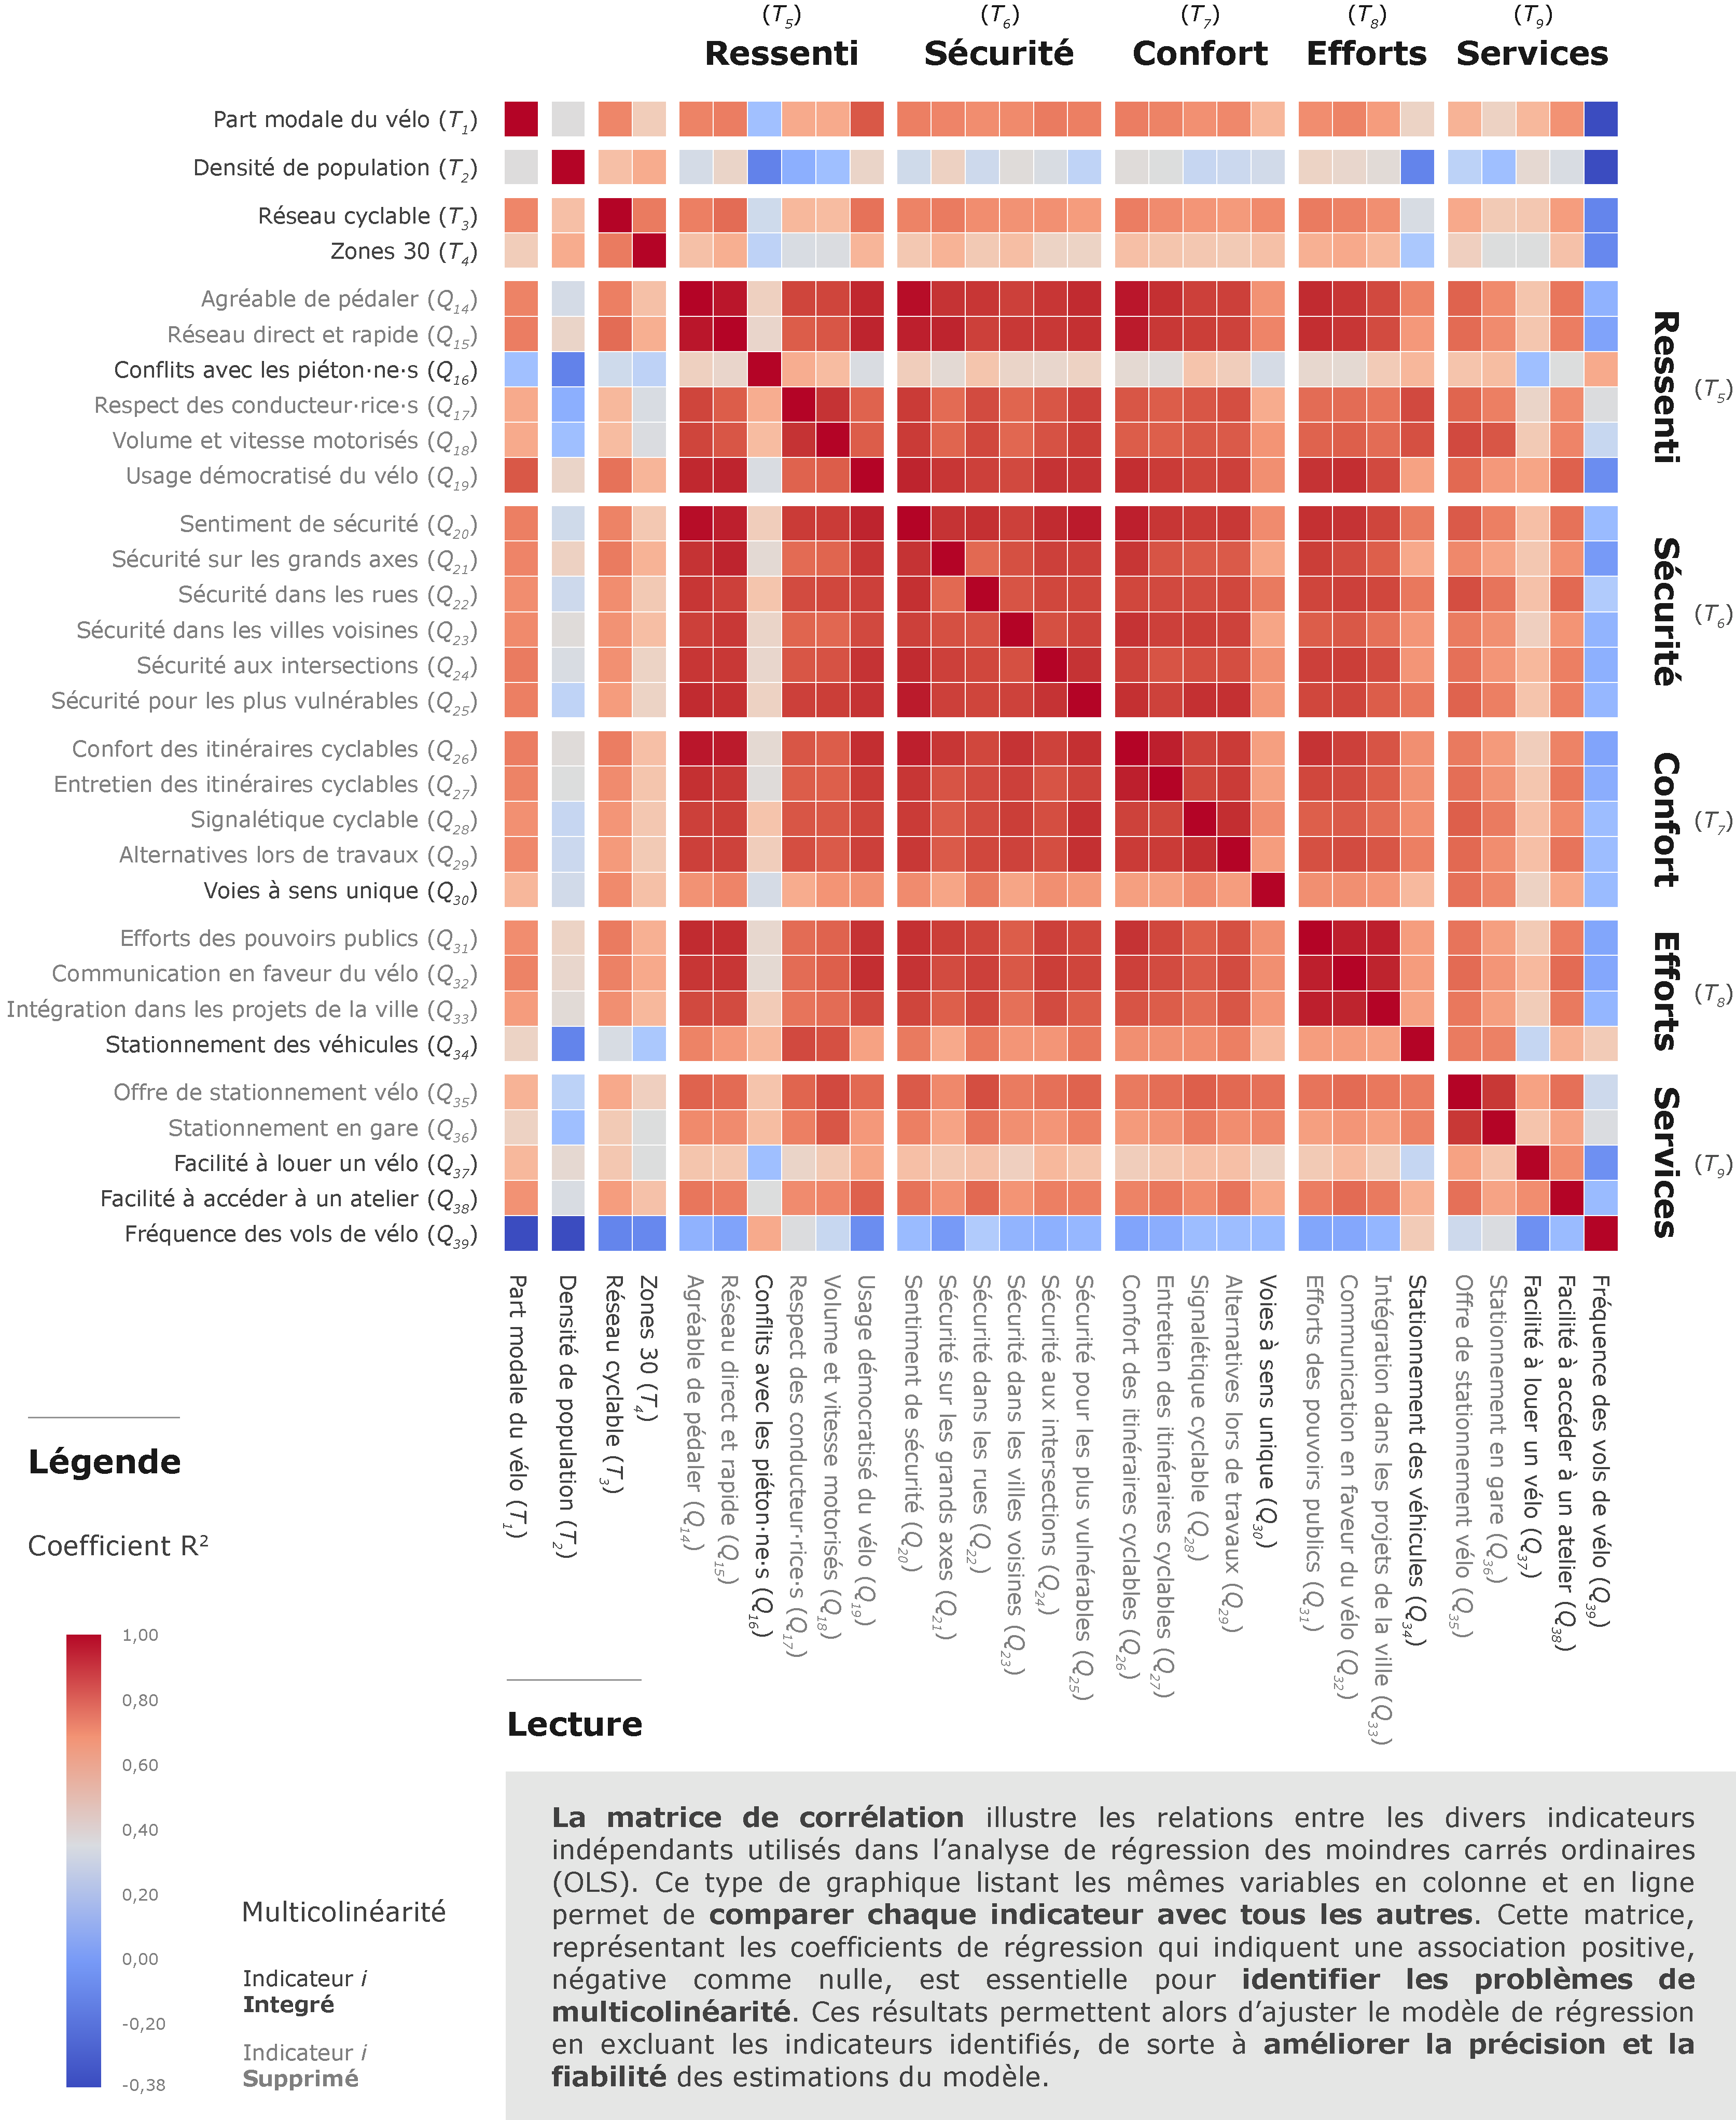
\includegraphics[width=1\columnwidth]{src/Figures/Chap-4/FR_Matrice_Autocorrelation_OLS.pdf}}
        \vspace{5pt}
        \begin{flushright}\scriptsize{
        Auteur~: \textcolor{blue}{Dylan Moinse (2023)}
        }\end{flushright}
    \end{figure}

    % Exclusion des colonnes
La base de données exploitée s'avère contenir plusieurs paires de variables fortement corrélées (\(VIF\)~\textless~10). Nous avons alors choisi d'exclure du modèle 21 indicateurs, étant donné que ceux-ci sont fortement corrélés avec plusieurs autres variables (voir \hyperref[fig-chap4:matrice-autocorrelation]{illustration~\ref{fig-chap4:matrice-autocorrelation}}, page~\pageref{fig-chap4:matrice-autocorrelation}). Dans ce contexte, nous avons conservé les colonnes indépendantes telles que la \Guillemets{part modale du vélo} (\(T_{1}\)), la \Guillemets{densité moyenne de population} (\(T_{2}\)), la \Guillemets{proportion d'itinéraires cyclables} (\(T_{3}\)), la \Guillemets{proportion de zones dont la vitesse motorisée est limitée à 30 km/h} (\(T_{4}\)) ainsi que les scores de \Guillemets{ressenti général} (\(T_{5}\)), de \Guillemets{sécurité} (\(T_{6}\)), de \Guillemets{confort} (\(T_{7}\)), liés aux \Guillemets{efforts de la ville} (\(T_{8}\)), aux \Guillemets{services et au stationnement} (\(T_{9}\)), aux \Guillemets{conflits avec les piéton·ne·s} (\(Q_{16}\)), aux \Guillemets{rues cyclables à sens unique} (\(Q_{30}\)), aux \Guillemets{véhicules sur les voies cyclables} (\(Q_{34}\)), à la \Guillemets{facilité de location de vélos} (\(Q_{37}\)), à la \Guillemets{facilité d'accès à un atelier de réparation} (\(Q_{38}\)) et aux \Guillemets{vols de vélos} (\(Q_{39}\)).%%Rédigé%%

    % Transition
Dans cette partie consacrée à la modélisation de la régression, nous avons préparé systématiquement les données et validé les hypothèses clés de la régression. Notre analyse confirme que le modèle de régression satisfait les hypothèses de normalité des résidus, d'homoscédasticité, et d'absence d'autocorrélation. En abordant ces éléments fondamentaux en statistiques, nous améliorons l'interprétabilité globale de nos résultats.%%Rédigé%%

    % 4.3.2.2.
    \needspace{1\baselineskip} % Réserve de l'espace
\subsubsection*{Validation du modèle
    \label{chap4:methodologie-validation}
    }

    % Introduction
Pour évaluer la performance prédictive de notre modèle de régression \acrshort{OLS}, nous avons calculé l'\acrfull{MSE}, ou \textsl{Mean Squarred Error}. La \acrshort{MSE} est une \gls{métrique} fréquemment utilisée pour évaluer la performance des modèles de régression \textcolor{blue}{\autocite{cochran_sampling_1963}}\index{Cochran, William~G.|pagebf}. Elle est déterminée en tant que moyenne des différences au carré entre les valeurs prédites et les valeurs réelles.%%Rédigé%%

    % Validation
Le facteur \acrshort{MSE} obtenu est une valeur extrêmement faible de 0,00127. Cela indique que les prédictions du modèle sont très proches des valeurs réelles. Une \acrshort{MSE} faible est effectivement souhaitable, car elle signifie des erreurs de prévision minimales, reflétant ainsi une grande précision du modèle.%%Rédigé%%

    % Coefficient
Le modèle de régression multivariée \acrshort{OLS} donne lieu à un coefficient de régression ($R^2$) de 0,765 et un coefficient de régression ajusté ($\bar{R}^2$) de 0,670, laissant supposer un bon ajustement du modèle. Cela revient à considérer que 76,5~\% de la variance de la variable dépendante, soit du taux de féminisation de la pratique cyclable, est expliquée par les variables indépendantes incluses dans le modèle.%%Rédigé%%

    % 4.3.3.
    \needspace{1\baselineskip} % Réserve de l'espace
\subsection{La cyclabilité mise en relation avec la pratique genrée de la mobilité individuelle légère
    \label{section-chap4:cyclabilite-territoires-genre}
    }

    %% Objectifs
Cette partie consacrée à la mobilité et au genre vise à explorer les relations existantes entre l'usage du vélo et de la micro-mobilité, l'environnement urbain et le genre en s'appuyant sur la cyclabilité telle que perçue par les cyclistes. À cette fin, une série d'objectifs prédéfinis oriente cette investigation statistique, comme suit~:
\begin{enumerate}
    \item En premier lieu, cette étude s'attache à quantifier les inégalités de genre concernant l'utilisation de la mobilité individuelle légère, du point de vue de la mobilité quotidienne. Cette étude cherche alors à s'appuyer sur un large échantillon d'individus à travers un périmètre géographique défini~;
    \item Une fois le tableau dressé, l'analyse interroge la place réelle occupée par la \Guillemets{sécurité par le nombre}\footnote{
Dans le contexte de la mobilité active, la \Guillemets{sécurité par le nombre} est un concept qui suggère que plus le nombre de cyclistes est important, plus cette pratique de mobilité devient sûre pour chaque usager·ère. Ce phénomène étudié peut s'expliquer en partie par une visibilité accrue sur la route, incitant les automobilistes à adopter un comportement de conduite plus prudent, mais également par une meilleure intégration dans les politiques d'aménagement et par un effet d'entraînement, une certaine masse critique encourageant l'adoption du vélo par de nouvelles personnes, améliorant dès lors la sécurité par le nombre de manière rétroactive.
} sur la compréhension de la répartition inégalitaire de l'usage de la micro-mobilité~;
    \item À l'issue de cette exploration statistique, l'évaluation de la cyclabilité ressentie comme paramètre venant influencer le choix modal de la mobilité individuelle légère permet d'éclairer les choix de mobilité au prisme du genre~;
    \item À travers une démarche comparative, cette sous-partie s'efforce de caractériser et de classifier les territoires étudiés, dans l'intérêt de mieux contextualiser les résultats énoncés~;
    \item Le dernier objectif vise à formuler un indicateur capable de saisir les principales interactions entre les variables examinées et l'usage différencié du vélo et de la micro-mobilité. Cet indice se présente comme un outil analytique, permettant de révéler les mécanismes sous-tendant la distribution genrée dans l'utilisation de la mobilité individuelle légère.
\end{enumerate}%%Rédigé%%

    %% Introduction
Cette section s'emploie à exposer les résultats qui se dégagent de cette analyse statistique, en éclairant les facteurs concourant à une plus grande équité dans l'usage du vélo et de la micro-mobilité. En premier lieu, cette recherche met l'accent sur les disparités de genre qui prévalent en France, tout comme dans notre étude régionale, en ce qui concerne l'adoption de la mobilité individuelle légère, qu'il s'agisse du vélo ou de la micro-mobilité émergente, tant en monomodalité qu'en intermodalité. À partir de ce constat, nous nous efforcerons de démontrer dans quelle mesure le concept de \Guillemets{sécurité par le nombre} entretient un lien avec la compréhension de ce phénomène social, sans prétendre toutefois en constituer le facteur direct. En effet, cette analyse statistique mettra en relief l'importance de la perception de la cyclabilité par les usager·ère·s, en commençant par la place de l'infrastructure cyclable et de la sécurité, éléments dépendant d'un ensemble formant ce que l'on peut qualifier de \Guillemets{système vélo}.%%Rédigé%%

    % 4.3.3.1.
    \needspace{1\baselineskip} % Réserve de l'espace
\subsubsection*{Un écart de genre manifeste dans l'usage du vélo et de la micro-mobilité en France
    \label{chap4:ecart-genre}
    }

    %% Usage genré monomodal
L'axe central de cette sous-section réside dans la mesure de la répartition genrée de l'usage du vélo et de la micro-mobilité en France. Sans grande surprise, l'analyse secondaire du fichier \textsl{MOBPro} met en lumière un déséquilibre démographique significatif concernant les déplacements à vélo. Cette base de données nationale sur la mobilité révèle que la participation féminine au vélo ne représente que 38,08~\% des usager·ère·s pour les déplacements domicile-travail dans le pays, comme le montre l'\hyperref[fig-chap4:part-modale-genree-mobilite-individuelle-legere]{illustration~\ref{fig-chap4:part-modale-genree-mobilite-individuelle-legere}} (page~\pageref{fig-chap4:part-modale-genree-mobilite-individuelle-legere}), alors même que les femmes constituent 51,60~\% de la population française \textcolor{blue}{\autocite{insee_documentation_2023}}\index{Insee@\textsl{Insee}|pagebf} et 58~\% des voyageur·se·s ferroviaires \textcolor{blue}{\autocite{enov_enquete_2021}}\index{Enov@\textsl{Enov}|pagebf}.%%Rédigé%%

    %% Figure Genre et types de micro-mobilité
    \begin{figure}[h!]\vspace*{4pt}
        \caption{Répartition de l'usage du vélo et de la micro-mobilité en fonction du genre déclaré et observé.}
        \label{fig-chap4:part-modale-genree-mobilite-individuelle-legere}
        \centerline{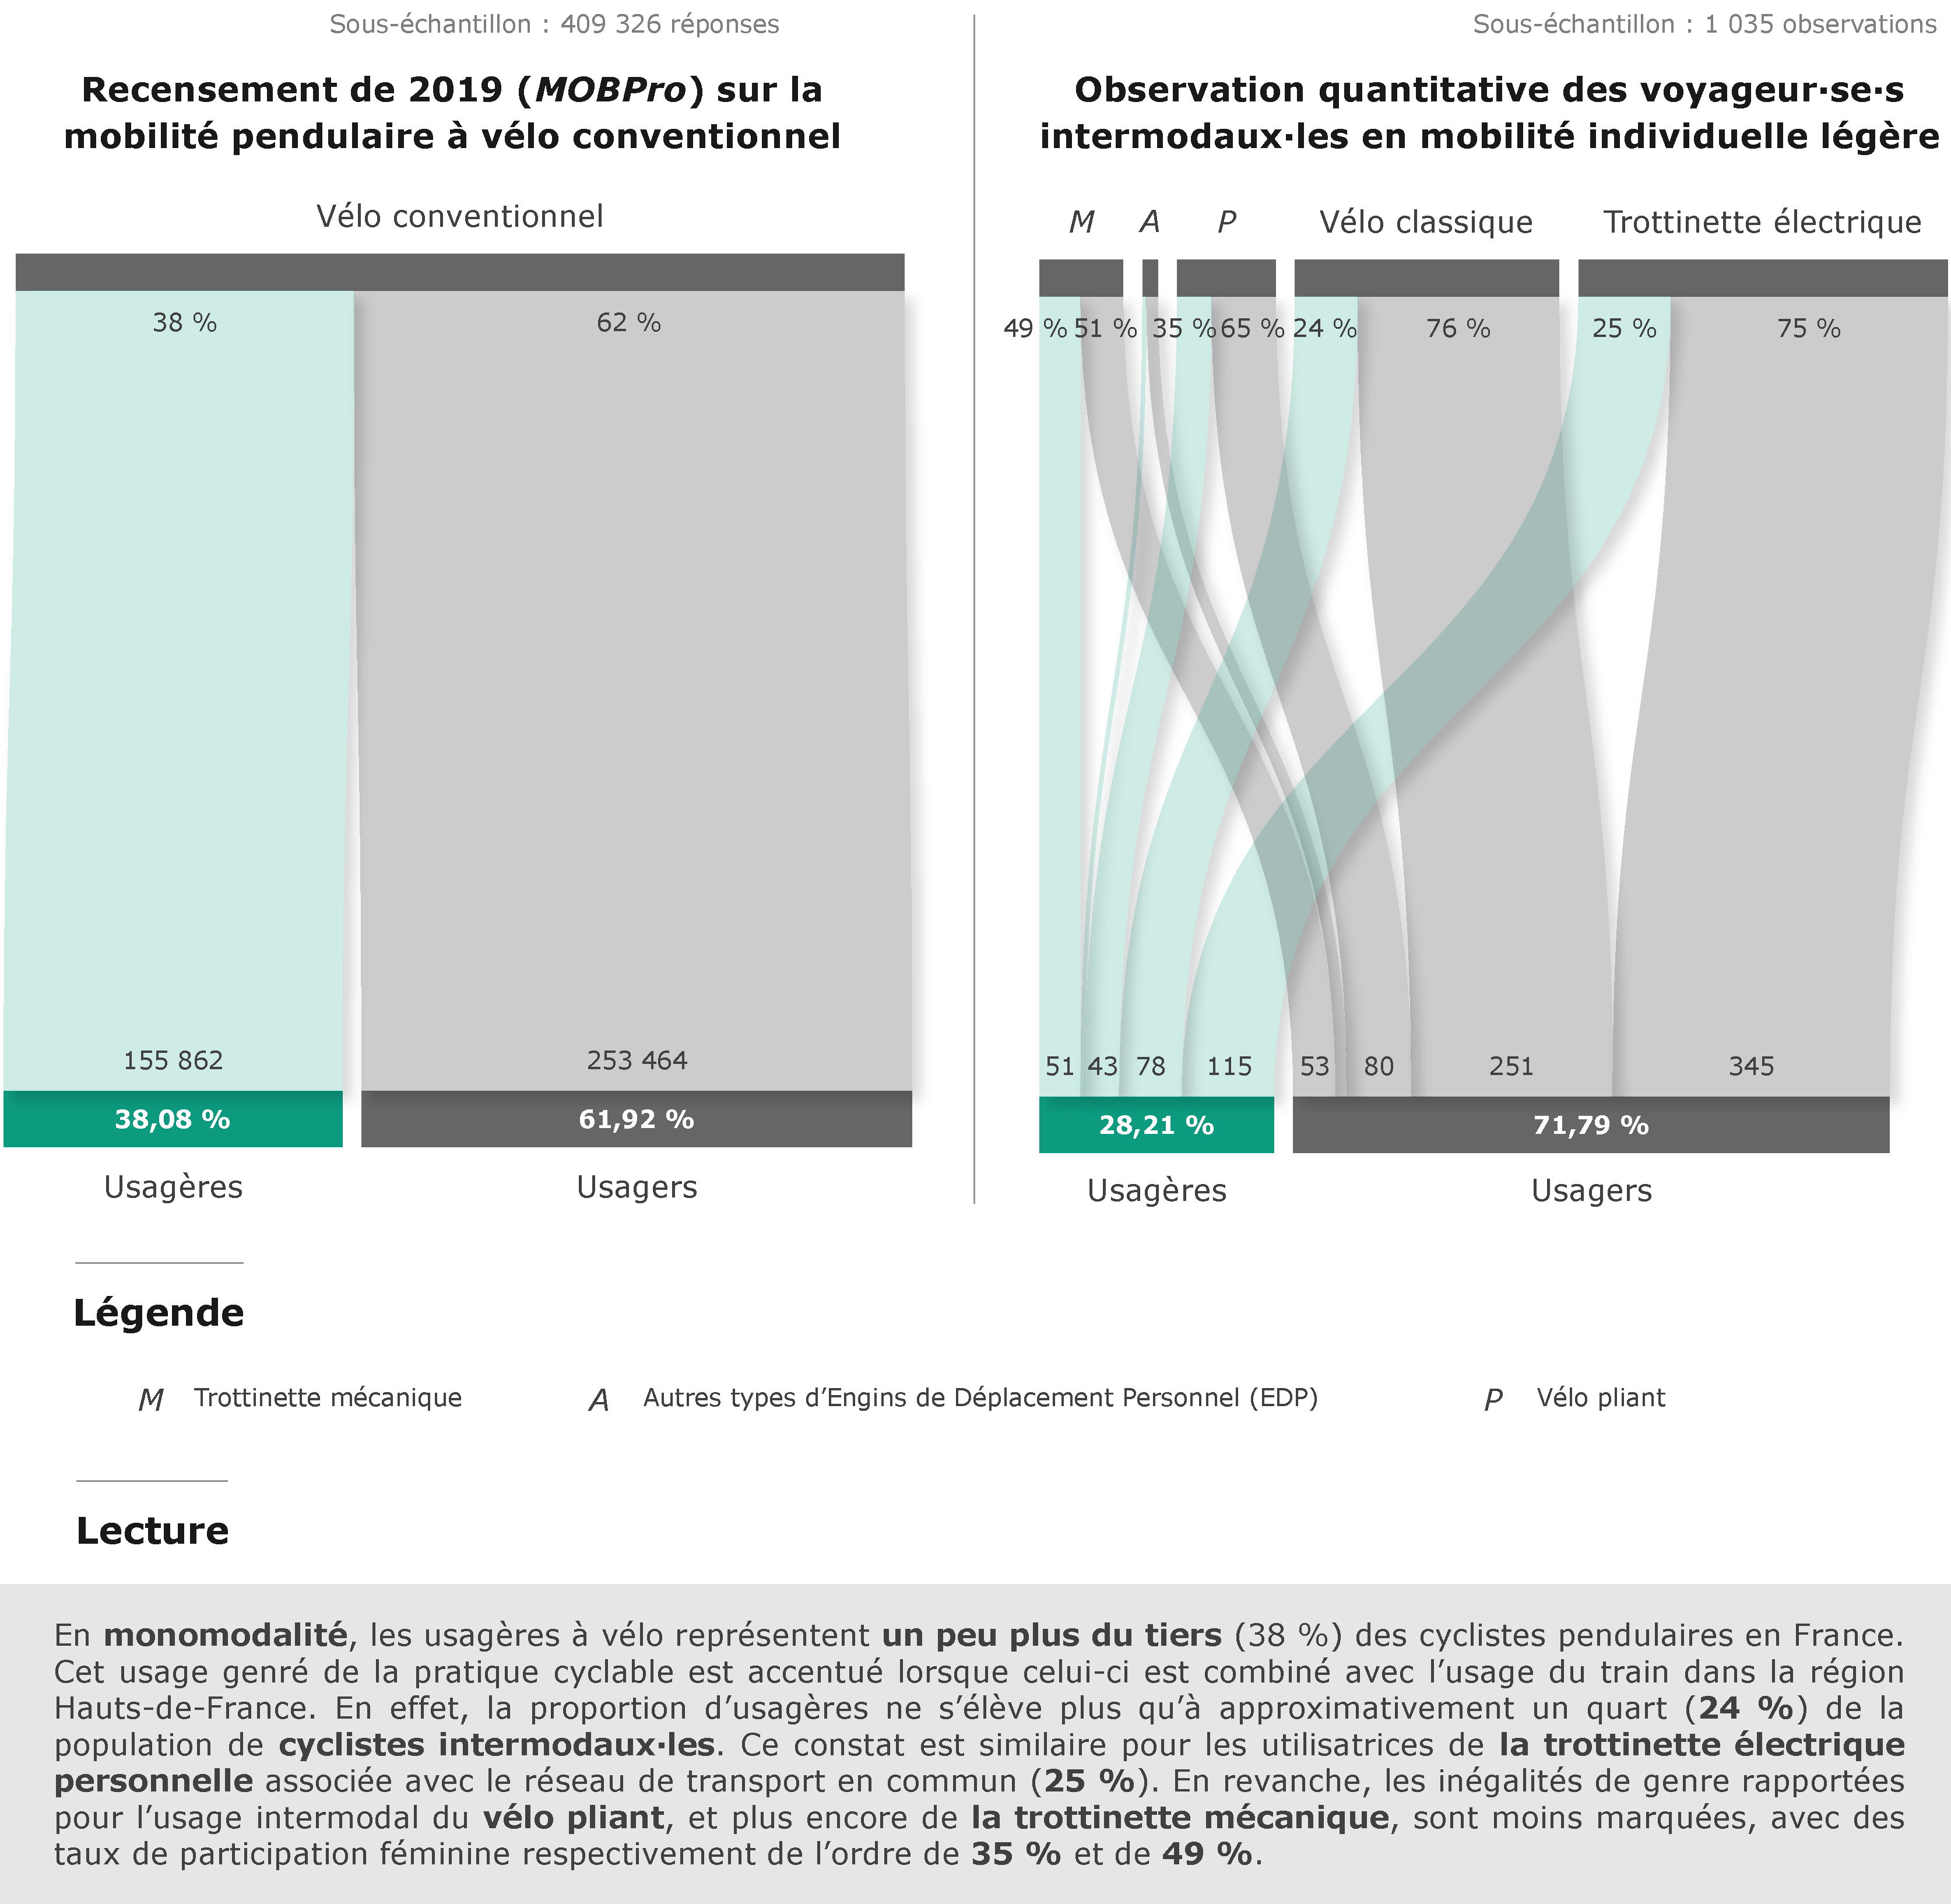
\includegraphics[width=1\columnwidth]{src/Figures/Chap-4/FR_Part_modale_genre_OLS.pdf}}
        \vspace{5pt}
        \begin{flushright}\scriptsize{
        Jeux de données~: \textsl{MOBPro} \textcolor{blue}{\autocite{insee_documentation_2023}}
        \\
        Auteur~: \textcolor{blue}{Dylan Moinse (2023)}
        }\end{flushright}
    \end{figure}

    % 4.3.3.2.
    \needspace{1\baselineskip} % Réserve de l'espace
\subsubsection*{Le rôle indirect de la masse critique de cyclistes dans la réduction des inégalités de genre
    \label{chap4:masse-critique-genre}
    }

    %% Part modale et usage genré
Cette évaluation statistique interroge tout d'abord, à l'échelle nationale, les liens entre le taux de participation féminine et la part modale du vélo au sein de cinquante-trois villes françaises. Le modèle de régression multivarié met en lumière la corrélation positive relativement significative entre le pourcentage de femmes pratiquant le vélo et l'usage généralisé du vélo dans les villes centres, avec un coefficient de détermination (noté $\hat{\beta}_{1}$) de 0,37 ($p$~\textless~0,05). Le concept de \Guillemets{sécurité par le nombre} implique de reconnaître que plus le nombre de cyclistes augmente dans l'espace public, plus les automobilistes ont tendance à les considérer comme un groupe légitime d'usager·ère·s de la route. En conséquence, les automobilistes deviennent plus attentif·ve·s aux cyclistes, comme l'expliquent \textcolor{blue}{\textcite[83]{oosteren_pourquoi_2021}}\index{Oosteren, Stein van|pagebf}\index{Schneider, Olivier|pagebf}, étant donné que la relation entre le nombre total de cyclistes et le nombre de cyclistes victimes d'accidents de la route est inversement proportionnelle \textcolor{blue}{\autocite[208]{jacobsen_safety_2003}}\index{Jacobsen, Peter Lyndon|pagebf}.%%Rédigé%%

    %% Figure Genre et part modale du vélo
    \begin{carte}[h!]\vspace*{4pt}
        \caption{Analyse croisée de la part modale et de la répartition genrée de l'usage du vélo en France.}
        \label{fig-chap4:carte-part-modale-velo-genre}
        \centerline{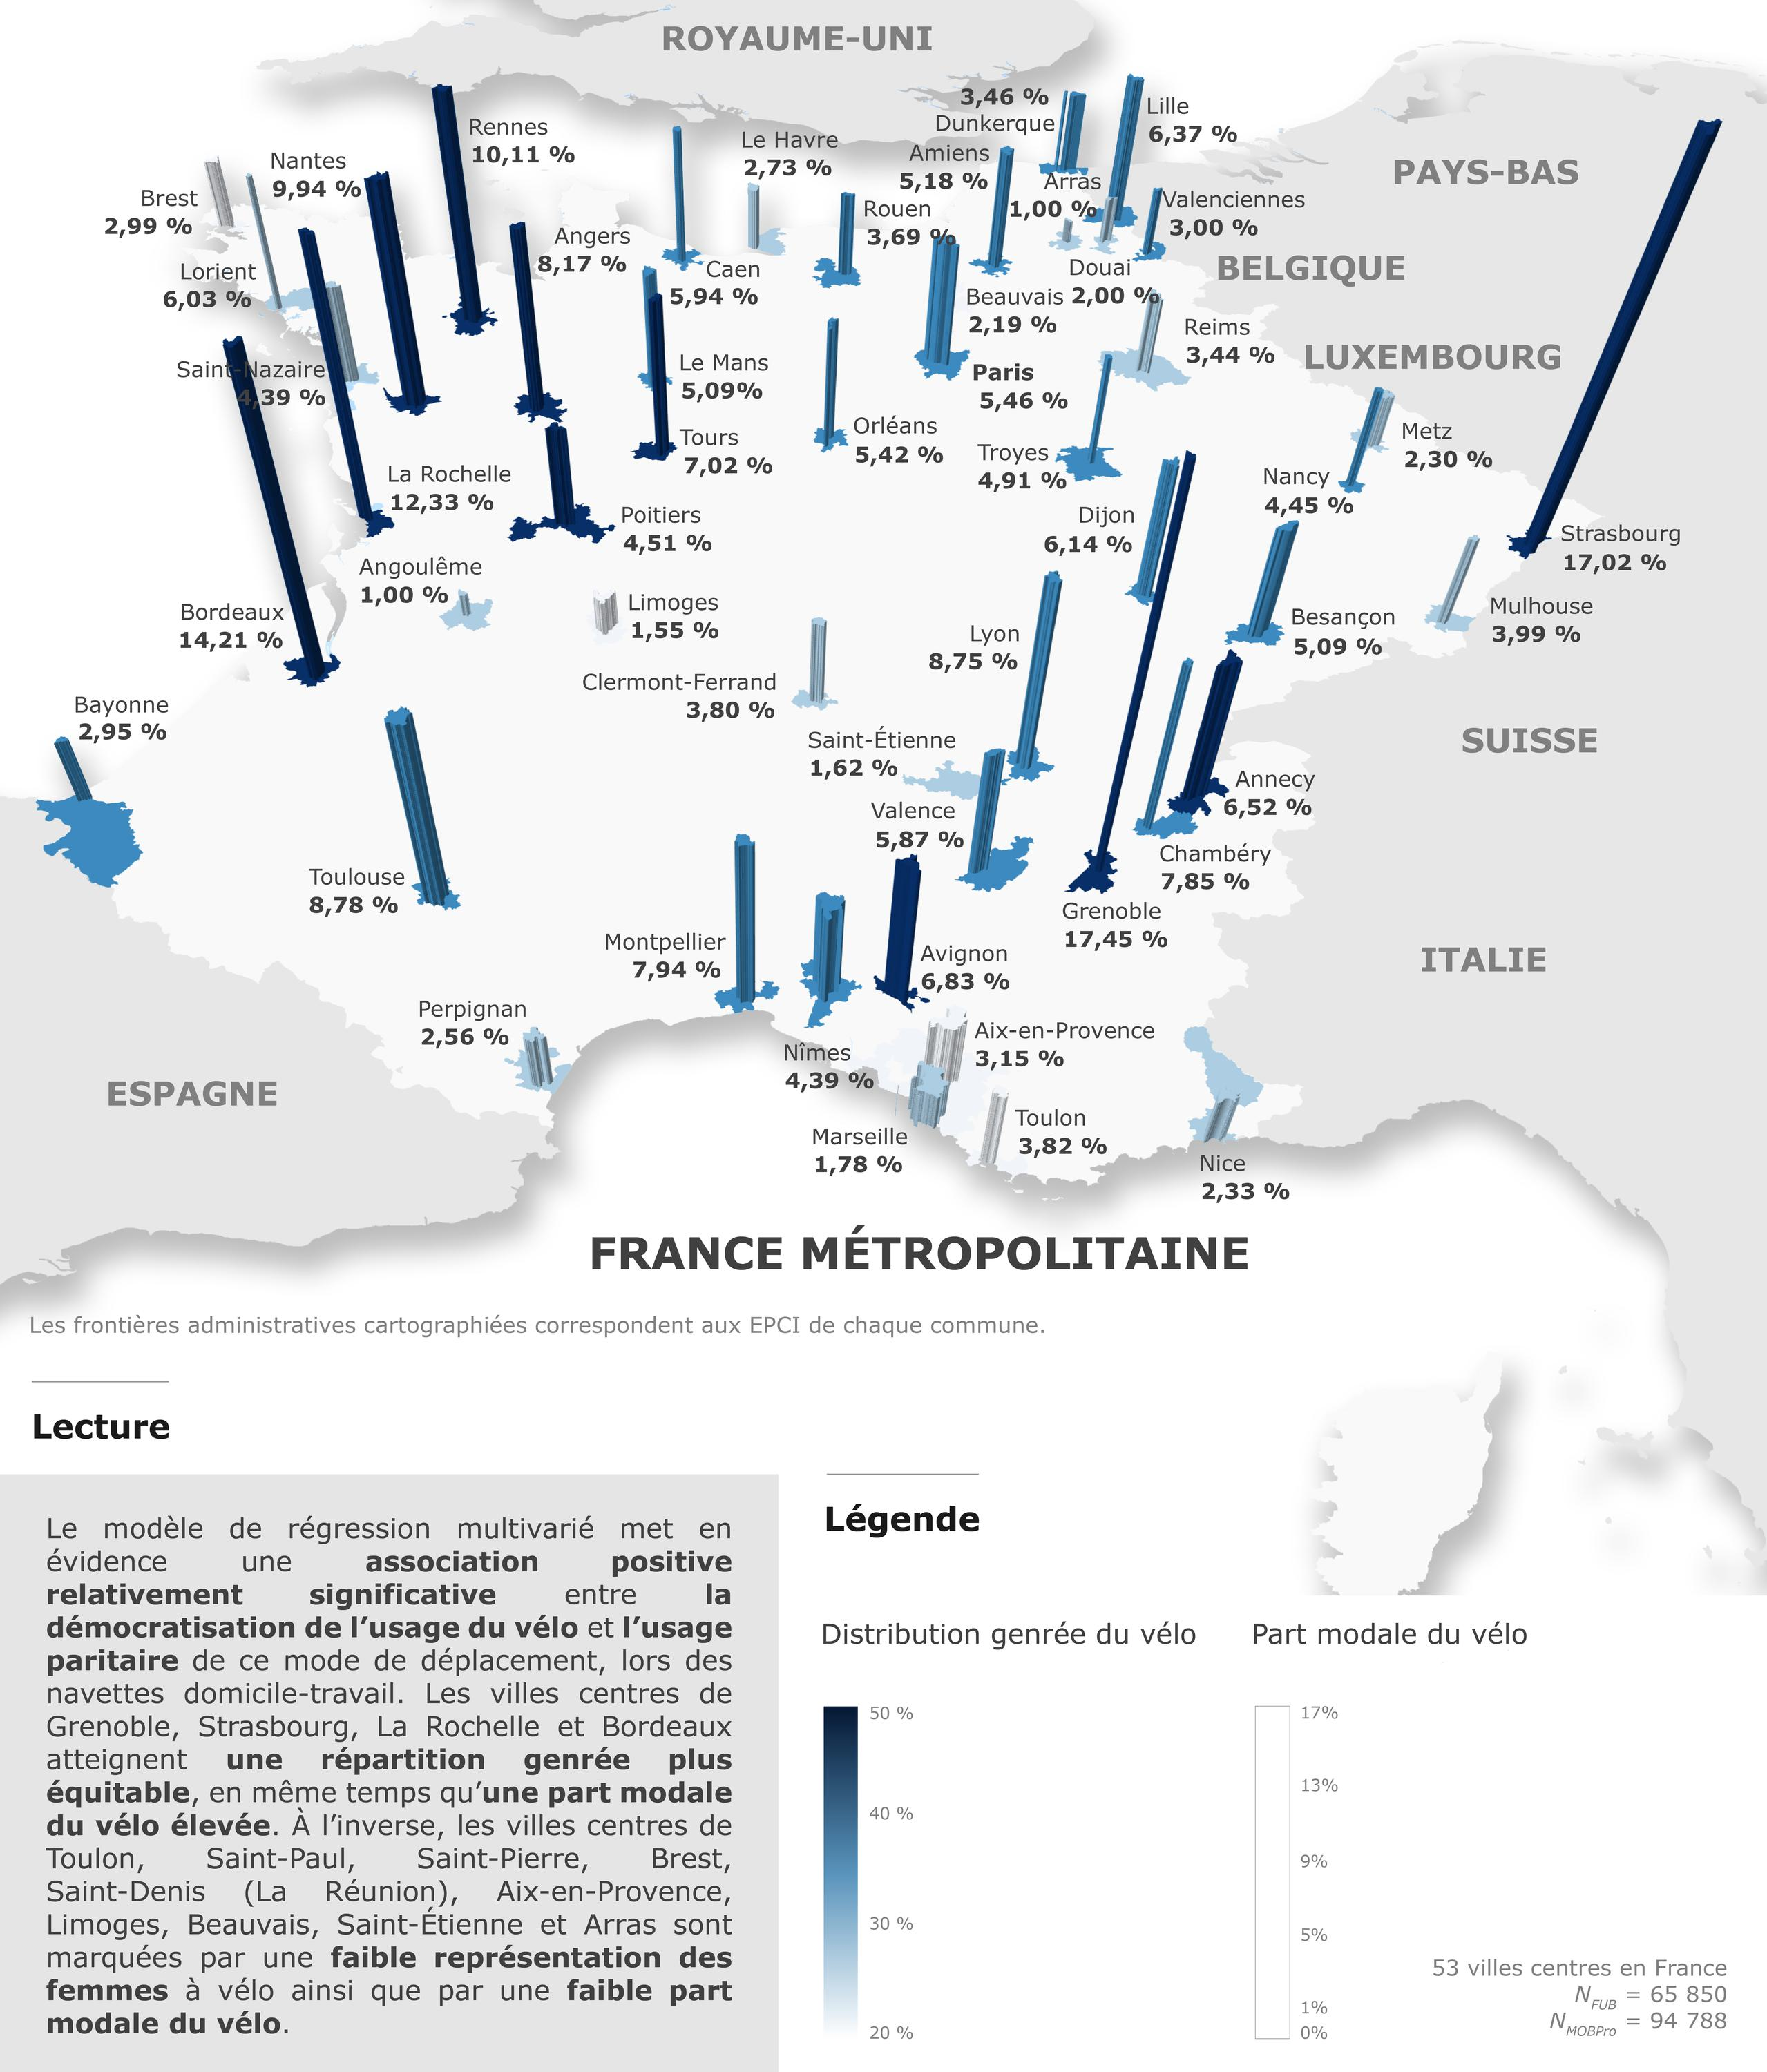
\includegraphics[width=1\columnwidth]{src/Figures/Chap-4/FR_Democratisation_velo_genre_OLS.jpg}}
        \vspace{5pt}
        \begin{flushright}\scriptsize{
        Jeux de données~: \textsl{MOBPro} \textcolor{blue}{\autocite{insee_documentation_2023}} et \textsl{Atlas Vélo Régional} \textcolor{blue}{\autocite{velo__territoires_atlas_2023}}
        \\
        Auteur~: \textcolor{blue}{Dylan Moinse (2023)}
        }\end{flushright}
    \end{carte}

    %% Exemples bons scores
Dans le domaine des villes renommées pour le développement considérable à l'égard du vélo en France, en particulier en ce qui concerne la part d'actif·ve·s qui optent pour le vélo, il convient de souligner une répartition genrée plus équitable. Notamment, à Grenoble et à Strasbourg, où la part modale atteint environ 17~\%, nous pouvons observer une représentation genrée dans ce mode de transport presque équilibrée, s'établissant respectivement à environ 45~\% et 49~\% (voir la \hyperref[fig-chap4:carte-part-modale-velo-genre]{carte~\ref{fig-chap4:carte-part-modale-velo-genre}}, page~\pageref{fig-chap4:carte-part-modale-velo-genre}). De même, La Rochelle et Bordeaux atteignent une parité genrée étroitement alignée sur leur population municipale (51~\%), tout en affichant des parts modales du vélo d'environ 12~\% et 14~\%.%%Rédigé%%

    %% Exemples mauvaises scores 
À l'inverse, certaines villes se caractérisent par une faible part modale du vélo, inférieure à la moyenne nationale de 3,5~\%, conjuguée à une faible représentation des femmes cyclistes. Parmi les villes les plus inégalitaires, citons notamment Toulon (20~\%), Saint-Paul (22~\%), Saint-Pierre (24~\%), Brest (25~\%), Saint-Denis de La Réunion (25~\%), Aix-en-Provence (26~\%), Limoges (26~\%), Beauvais (28~\%), Saint-Étienne (28~\%) et Arras (28~\%), où la part modale du vélo oscille entre 1~\% et 3~\% (voir la \hyperref[fig-chap4:carte-part-modale-velo-genre]{carte~\ref{fig-chap4:carte-part-modale-velo-genre}}, page~\pageref{fig-chap4:carte-part-modale-velo-genre}). Néanmoins, il est nécessaire de nuancer ces observations en tenant compte de contre-exemples spécifiques qui ne semblent pas répondre à ce modèle de régression linéaire. Des villes telles qu'Avignon (50~\%), Poitiers (45~\%), Valenciennes (42~\%) et Bayonne (37~\%) se démarquent en étant caractérisées par des disparités liées au genre moins prononcées, malgré une part modale modeste du vélo, établie entre 3~\% et 7~\%.%%Rédigé%%

    %% Observation quantitative
La corrélation positive déterminée entre la part modale et la participation féminine au vélo demeure cohérente, mais apparaît bien moins significative, lorsque nous considérons l'utilisation intermodale de la micro-mobilité dans l'étude de cas des Hauts-de-France. Le modèle de régression linéaire produit un coefficient de 0,25 ($p$~\textless~0,05) lors de l'analyse des données des neuf gares ferroviaires enquêtées. À la gare centrale de Lille Flandres et à la gare périurbaine de Lille CHR, où la part modale du vélo dans la commune est de 6,1~\%, les voyageur·se·s ayant recours à cette combinaison modale avec le vélo conventionnel comprennent moins d'un tiers de femmes (31,70~\% sur 287 observations et 31,97~\% sur 122 observations). Une répartition genrée similaire est observée à la gare d'Armentières (31,72~\% sur 145 observations) dans une commune pourtant parcourue par 4~\% de cyclistes pendulaires. La courbe de tendance est ensuite influencée par les gares de Béthune (21,88~\% sur 32 observations), Lesquin (15,79~\% sur 22 observations), Creil (12,5~\% sur 32 observations) et Dunkerque (12,24~\% sur 49 observations), où la part modale du vélo varie de 1~\% à 3~\%. Lors de la différenciation entre les types de mobilité individuelle légère, une relation modérément significative est observée ($\hat{\beta}$~=~0,23,~$p$~\textless~0,05) pour l'utilisation intermodale du vélo classique, tandis qu'une relation faible est constatée pour la \acrshort{TEP} combinée avec les réseaux de transport en commun ($\hat{\beta}$~=~0,17,~$p$~\textless~0,05). En revanche, cette relation n'est pas significative pour le vélo pliant et la trottinette mécanique. Nous proposons à ce stade, de confronter l'analyse quantitative aux appréciations émises au travers de notre protocole qualitatif.%%Rédigé%%

    %% Parcours commentés
La primauté accordée à la notion de \Guillemets{sécurité par le nombre} dans la pratique de la mobilité individuelle légère se manifeste dans l'examen des parcours commentés mis en œuvre. La participante désignée sous le nom de \(PCTE_{1}\) articule une perspective nuancée concernant la cohabitation des usager·ère·s de la \acrshort{TEP} avec le trafic automobile, dans les quartiers de gare parcourus. Cette dernière identifie le partage de la voirie comme un obstacle majeur à l'adoption de ce mode de déplacement. La participante compare diverses expériences de mobilité en soulignant une familiarisation progressive des automobilistes avec la \acrshort{TEP}, \Guillemets{\textsl{habitué·e·s à ce mode de transport}} [17:40, \(PCTE^{TC}_{1}\)] dans le contexte lillois. Ces interactions contrastent nettement avec son ressenti à Maubeuge, où l'usagère exprime un sentiment d'insécurité et de décalage, ayant alors \Guillemets{\textsl{l'impression d'être un OVNI}}~dans cet environnement urbain [17:40, \(PCTE^{TC}_{1}\)]. La mention de la visibilité des cyclistes réapparaît lors de la description de son itinéraire en post-acheminement à Maubeuge, au cours desquels la participante insiste sur le fait que les \Guillemets{\textsl{voitures ne} [soient] \textsl{pas hyper habituées à tout ce qui est trottinette ou vélo. C'est une petite bande cyclable sur la montée, mais j'ai peur que les voitures ne fassent pas attention}}. Ce témoignage, en plus de conforter l'importance de la masse critique de cyclistes dans les espaces publics, démontre que la seule présence de bandes cyclables ne permet pas à la participante de se sentir en sécurité en trottinette électrique (voir l'\hyperref[fig-chap4:pcte1e-partage-voirie]{extrait vidéo~\ref{fig-chap4:pcte1e-partage-voirie}}, page~\pageref{fig-chap4:pcte1e-partage-voirie}). Elle évoque toutefois la présence de quelques usager·ère·s en trottinette électrique dans la commune, une observation qui \Guillemets{[la] \textsl{rassure.} [\dots] \textsl{les automobilistes connaissent un petit peu} [les trottinettes circulant sur la voie]. \textsl{Même si rien que les vélos, il n'y en a pas énormément.}}~[17:40, \(PCTE^{TC}_{1}\)].%%Rédigé%%

    %% Figure 1 PCTE1E Maubeuge
    \begin{figure}[h!]\vspace*{4pt}
        \caption{Image extraite de l'itinéraire filmé en diffusion depuis la gare de Maubeuge et illustrant la présence d'un virage jugé dangereux en fin de voie (\(PCTE^{E}_{1}\)).}
        \label{fig-chap4:pcte1e-partage-voirie}
        \centerline{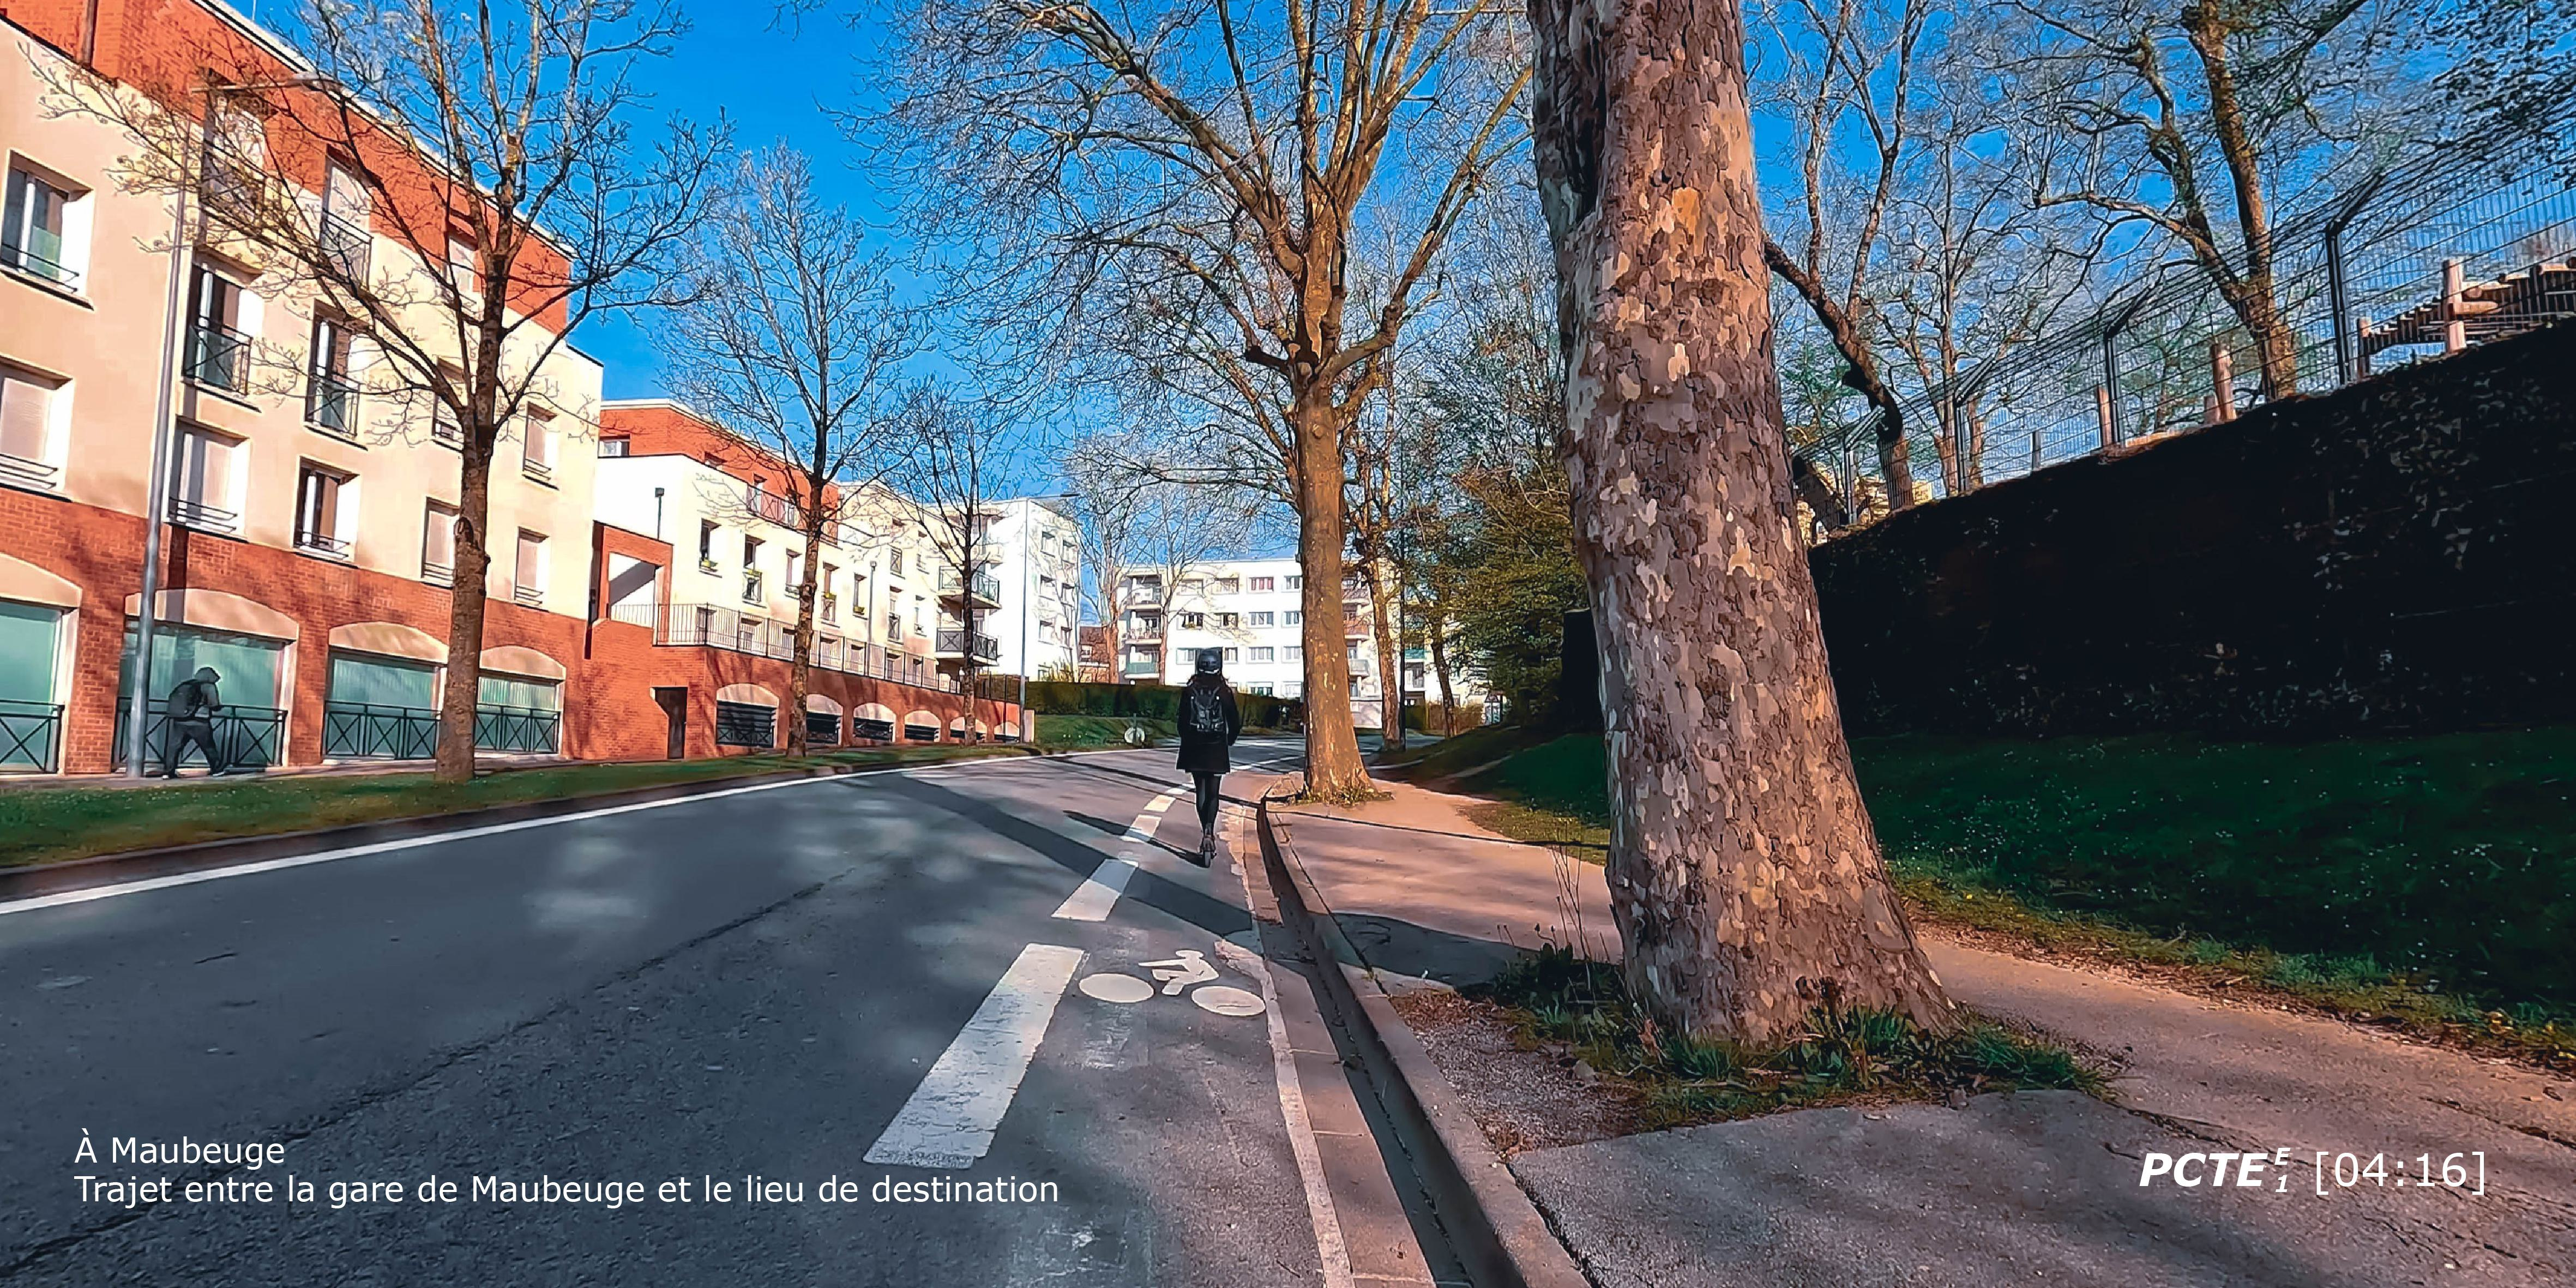
\includegraphics[width=1\columnwidth]{src/Figures/Chap-4/Extrait_Video_PCTE1_Egress_9.jpg}}
        \vspace{5pt}
        \begin{flushright}\scriptsize{
        Auteur~: \textcolor{blue}{Dylan Moinse (2022)}
        }\end{flushright}
    \end{figure}

    %% Discussion littérature
À notre connaissance, le rôle primordial de la masse critique de cyclistes dans la participation féminine à la mobilité individuelle légère n'a pas encore été démontré de manière statistique dans le contexte français, à l'exception de Strasbourg où la part modale du vélo dépasse 17~\% et où les femmes représentent 48~\% des cyclistes \textcolor{blue}{\autocite[42]{certu_usagers_2013}}\index{Certu@\textsl{Certu}|pagebf}. Certaines observations formulées par \textcolor{blue}{Frédéric} \textcolor{blue}{\textcite[187]{heran_retour_2015}}\index{Héran, Frédéric|pagebf} et \textcolor{blue}{Thibaut} \textcolor{blue}{\textcite{schepman_pourquoi_2014}}\index{Schepman, Thibaut|pagebf} suggèrent qu'une forte présence de cyclistes dans une commune a tendance à favoriser un usage du vélo plus équitable, citant des exemples tels que Strasbourg et Copenhague. Ces résultats sont alors en accord avec la comparaison internationale menée par \textcolor{blue}{\textcite[63]{garrard_revolutions_2006}}\index{Garrard, Jan|pagebf}\index{Crawford, Sharyn|pagebf}\index{Hakman, Natalie|pagebf}, qui ont souligné que les pays affichant des taux élevés d'usage du vélo, que ce soit pour les trajets domicile-travail ou les loisirs, ont tendance à connaître des différences de genre réduites en ce qui concerne cette forme de mobilité active. De manière similaire, dans une analyse portant sur dix-sept pays répartis sur six continents, \textcolor{blue}{\textcite[70]{goel_cycling_2022}}\index{Goel, Rahul|pagebf}\index{Goodman, Anna|pagebf}\index{Aldred, Rachel|pagebf}\index{Nakamura, Ryota|pagebf}\index{Tatah, Lambed|pagebf}\index{Garcia, Leandro Martin Totaro|pagebf}\index{Zapata-Diomedi, Belen|pagebf}\index{Sa, Thiago Herick de|pagebf}\index{Tiwari, Geetam|pagebf}\index{Nazelles, Audrey de|pagebf}\index{Tainio, Marko|pagebf}\index{Buehler, Ralph|pagebf}\index{Götschi, Thomas|pagebf}\index{Woodcock, James|pagebf} ont identifié une corrélation positive entre la démocratisation du vélo d'une part, et la propension pour les femmes de se déplacer à vélo d'autre part. De plus, dans les communes et les pays où la part modale du vélo est inférieure à 7~\%, les femmes présentent en moyenne une probabilité de pratiquer le vélo inférieure de 56~\% à celle des hommes, comme l'ont montré \textcolor{blue}{\textcite[70]{goel_cycling_2022}}\index{Goel, Rahul|pagebf}\index{Goodman, Anna|pagebf}\index{Aldred, Rachel|pagebf}\index{Nakamura, Ryota|pagebf}\index{Tatah, Lambed|pagebf}\index{Garcia, Leandro Martin Totaro|pagebf}\index{Zapata-Diomedi, Belen|pagebf}\index{Sa, Thiago Herick de|pagebf}\index{Tiwari, Geetam|pagebf}\index{Nazelles, Audrey de|pagebf}\index{Tainio, Marko|pagebf}\index{Buehler, Ralph|pagebf}\index{Götschi, Thomas|pagebf}\index{Woodcock, James|pagebf}.%%Rédigé%%

    %% Transition
Cette deuxième phase d'analyse statistique a permis d'établir un lien significatif entre la proportion de cyclistes et l'inclination des femmes à adopter le vélo d'un point de vue géographique. Cependant, cette corrélation significative ne fournit pas d'indications sur les relations causales entre ces deux variables. En particulier, il demeure incertain de conclure si l'influence de la masse critique favorise effectivement une plus grande diversité genrée parmi les cyclistes, ou s'il s'agit finalement de la participation accrue des femmes qui tend à augmenter la part modale de ce mode de déplacement, ou encore la réunion des deux facteurs qui opèrent de manière interactive. C'est dans cette perspective et dans le cadre de notre positionnement scientifique concernant le rôle de l'agencement territorial que cette étude a cherché à évaluer le rôle de la cyclabilité.%%Rédigé%%
    
    % 4.3.3.3.
    \needspace{1\baselineskip} % Réserve de l'espace
\subsubsection*{Aborder les inégalités de genre dans la mobilité à la lumière de la cyclabilité
    \label{chap4:cyclabilite-genre}
    }

    %% Associations liées à l'environnement urbain
Au travers de l'approche comparative menée dans les 53 villes centres, le modèle de régression met en avant une association positive entre l'usage genré du vélo et la part d'aménagements cyclables au sein de chaque commune ($\hat{\beta}_{3}$~=~0,60,~$p$~\textless~0,01). En revanche, la corrélation entre la part de zones~30 et la répartition genrée du vélo n'est pas statistiquement significative ($\hat{\beta}_{4}$~=~-0,12,~$p$~\texttt{>}~0,10), de manière similaire à la densité de population, qui ne présente pas de relation discernable ($\hat{\beta}_{2}$~=~-0,17,~$p$~\texttt{>}~0,10). Les résultats confirment dès lors les liens importants entre la part modale du vélo et la cyclabilité objective \textcolor{blue}{\autocite[8]{codina_built_2022}}\index{Codina, Oriol|pagebf}\index{Maciejewska, Monika|pagebf}\index{Nadal, Jordi|pagebf}\index{Marquet, Oriol|pagebf} qui influencent l'usage genré du vélo (voir le \hyperref[table-chap4:regression-genre-barometre-fub]{tableau~\ref{table-chap4:regression-genre-barometre-fub}}, page~\pageref{table-chap4:regression-genre-barometre-fub}).%%Rédigé%%

    % Tableau Résultats de la régression OLS
% Résultats de la régression OLS
%%Rédigé%%
    \begin{table}[h!]
    \centering
    \renewcommand{\arraystretch}{1.5}
    \resizebox{\columnwidth}{!}{
    \begin{tabular}{p{0.07\columnwidth}p{0.39\columnwidth}p{0.09\columnwidth}p{0.07\columnwidth}p{0.08\columnwidth}p{0.07\columnwidth}p{0.07\columnwidth}p{0.09\columnwidth}p{0.07\columnwidth}}
        %\hline
    \rule{0pt}{15pt} \small{\textcolor{blue}{\textbf{ID}}} & \small{\textcolor{blue}{\textbf{Variables indépendantes}}} & \small{\textcolor{blue}{\textbf{$\hat{\beta}$}}} & \small{\textcolor{blue}{\textbf{$\sigma$}}} & \small{\textcolor{blue}{\textbf{\(t_{stat}\)}}} & \small{\textcolor{blue}{\textbf{$p$}}} & \small{\textcolor{blue}{\textbf{\(VIF\)}}} & \small{\textcolor{blue}{\textbf{\(IC_{inf}\)}}} & \small{\textcolor{blue}{\textbf{\(IC_{sup}\)}}}\\
        \hline
\(T_{1}\) & \underline{\small{Part modale du vélo}} & \small{0,37} & \small{0,17} & \small{2,12} & \small{0,04} & \small{4,73} & \small{0,02} & \small{0,72} \\
\(T_{2}\) & \small{Densité de population} & \small{-0,17} & \small{0,14} & \small{-1,16} & \small{0,25} & \small{3,28} & \small{-0,46} & \small{0,13} \\
\(T_{3}\) & \underline{\small{Réseau cyclable}} & \small{0,60} & \small{0,22} & \small{2,72} & \small{0,01} & \small{7,56} & \small{0,15} & \small{1,04} \\
\(T_{4}\) & \small{Proportion de zones~30} & \small{-0,12} & \small{0,16} & \small{-0,76} & \small{0,45} & \small{3,94} & \small{-0,44} & \small{0,20} \\
\(T_{5}\) & \underline{\small{\textsl{Ressenti général}}} & \small{0,96} & \small{0,54} & \small{1,78} & \small{0,05} & \small{5,89} & \small{-0,14} & \small{2,05} \\
\(T_{6}\) & \small{\textsl{Sécurité}} & \small{-0,75} & \small{0,60} & \small{-1,25} & \small{0,22} & \small{6,99} & \small{-1,97} & \small{0,47} \\
\(T_{7}\) & \small{\textsl{Confort}} & \small{-0,65} & \small{0,36} & \small{-1,83} & \small{0,08} & \small{4,03} & \small{-1,37} & \small{0,07} \\
\(T_{8}\) & \underline{\small{\textsl{Efforts de la ville}}} & \small{0,58} & \small{0,26} & \small{2,19} & \small{0,04} & \small{2,94} & \small{0,04} & \small{1,11} \\
\(T_{9}\) & \small{\textsl{Services et stationnement}} & \small{-0,22} & \small{0,34} & \small{-0,65} & \small{0,52} & \small{8,57} & \small{-0,92} & \small{0,47} \\
\(Q_{16}\) & \small{Conflits avec les piéton·ne·s} & \small{-0,31} & \small{0,17} & \small{-1,86} & \small{0,07} & \small{4,35} & \small{-0,65} & \small{0,03} \\
\(Q_{30}\) & \small{Rues cyclables à sens unique} & \small{0,22} & \small{0,20} & \small{1,12} & \small{0,27} & \small{5,97} & \small{-0,18} & \small{0,61} \\
\(Q_{34}\) & \small{Véhicules sur les voies} & \small{0,07} & \small{0,23} & \small{0,29} & \small{0,77} & \small{8,51} & \small{-0,40} & \small{0,54} \\
\(Q_{37}\) & \small{Facilité de location} & \small{0,32} & \small{0,24} & \small{1,36} & \small{0,18} & \small{8,86} & \small{-0,16} & \small{0,80} \\
\(Q_{38}\) & \small{Facilité d'accès à un atelier} & \small{-0,22} & \small{0,19} & \small{-1,20} & \small{0,24} & \small{5,37} & \small{-0,60} & \small{0,15} \\
\(Q_{39}\) & \small{Vols de vélos} & \small{0,07} & \small{0,18} & \small{0,38} & \small{0,70} & \small{5,11} & \small{-0,30} & \small{0,43} \\
        \hline
        \end{tabular}}
    \caption{Caractérisation des relations entre la participation des femmes au vélo et les variables indépendantes définies dans le modèle de régression des moindres carrés ordinaires.}
    \label{table-chap4:regression-genre-barometre-fub}
        \vspace{5pt}
        \begin{flushleft}\scriptsize{
        \textcolor{blue}{Note~:} la colonne~$\hat{\beta}$~représente le coefficient de régression, $\sigma$ l'erreur standard, \(t_{stat}\) la statistique $t$ ($\hat{\beta}/\sigma$), $p$ la valeur~$p$ (\underline{significative} lorsqu'elle est inférieure ou égale à 0,05), \(VIF\) le facteur d'inflation de la variance, \(IC_{inf}\) et \(IC_{sup}\) les intervalles de confiance.
        \\
        \textcolor{blue}{Lecture~:} la modélisation nous permet d'affirmer que la part modale du vélo, la densité du réseau cyclable et les efforts de la ville ont un effet significatif et positif sur la participation féminine au vélo. La sécurité et le confort, dont les coefficients sont non significatifs, suggèrent une influence moins claire sur le choix modal du vélo par les femmes.
        }\end{flushleft}
        \begin{flushright}\scriptsize{
        Jeux de données~: \textsl{Baromètre des Villes Cyclables} \textcolor{blue}{\autocite{fub_barometre_2021}} et \textsl{OpenStreetMap} \textcolor{blue}{\autocite{openstreetmap_openstreetmap_2023}}
        \\
        Auteur~: \textcolor{blue}{Dylan Moinse (2023)}
        }\end{flushright}
        \end{table}%%Rédigé%%

    %% Régression linéaire générale
En parallèle, l'identification d'une corrélation notablement positive entre le score de cyclabilité perçue parmi les cyclistes en France et la pratique féminine du vélo parmi les villes sélectionnées s'avère significative, que ce soit pour les villes centres intégrées au sein d'une Métropole, d'une \acrfull{CU} ou d'une \acrfull{CA}\footnote{
    Ces trois types d'intercommunalité sont liés à la démographie, à la structure administrative et à la gouvernance française, connus sous le nom d'\acrfull{EPCI} à fiscalité propre. Ces entités administratives, conçues pour regrouper plusieurs municipalités, sont principalement catégorisées en fonction de la taille de la population de l'\acrshort{EPCI}. En conséquence, suite à la Réforme territoriale française de 2010, la classification des \acrshort{EPCI} à fiscalité propre comprend la \acrfull{CC} (au moins 15~000 habitant·e·s), la \acrfull{CA} (au moins 50~000 habitant·e·s), la \acrfull{CU} (au moins 250~000 habitant·e·s) et la Métropole (au moins 400~000 habitant·e·s).
}. Ce constat est d'autant plus vérifié pour le \Guillemets{ressenti général} (\(T_{5}\)) qui détient un coefficient de 0,96 ($p$~\textless~0,05), comme l'indique le \hyperref[table-chap4:regression-genre-barometre-fub]{tableau~\ref{table-chap4:regression-genre-barometre-fub}} (page~\pageref{table-chap4:regression-genre-barometre-fub}). Toutes choses égales par ailleurs, il apparaît qu'un usage paritaire du vélo est atteint lorsque la note de cyclabilité perçue d'une ville dépasse la note de 4,3/6, comme le souligne l'\hyperref[fig-chap4:regression-genre-cyclabilite]{illustration~\ref{fig-chap4:regression-genre-cyclabilite}} (page~\pageref{fig-chap4:regression-genre-cyclabilite}). Parmi les trois villes marquées par un usage égalitaire du vélo du point de vue du genre, La Rochelle et Bordeaux obtiennent respectivement des scores de 4,13 et 3,42, tandis qu'Avignon enregistre un score de 3,13, se rapprochant de la note moyenne des 53 villes, qui est de 3,08. Dans un contexte plus large, les sept villes~–~Bordeaux, Avignon, La Rochelle, Strasbourg, Annecy, Grenoble et Tours~–~marquées par un taux de représentation féminine dépassant les 45~\%, affichent une note moyenne de 3,74. En revanche, les dix communes dans lesquelles le vélo est principalement dominé par les hommes, avec une proportion excédant les 70~\%, obtiennent une note moyenne de 2,63.%%Rédigé%%

    %% Figure régression linéaire cyclabilité et genre
    \begin{figure}[h!]\vspace*{4pt}
        \caption{Modèle de régression linéaire entre la proportion de femmes à vélo et en micro-mobilité et la cyclabilité perçue des villes centres françaises.}
        \label{fig-chap4:regression-genre-cyclabilite}
        \centerline{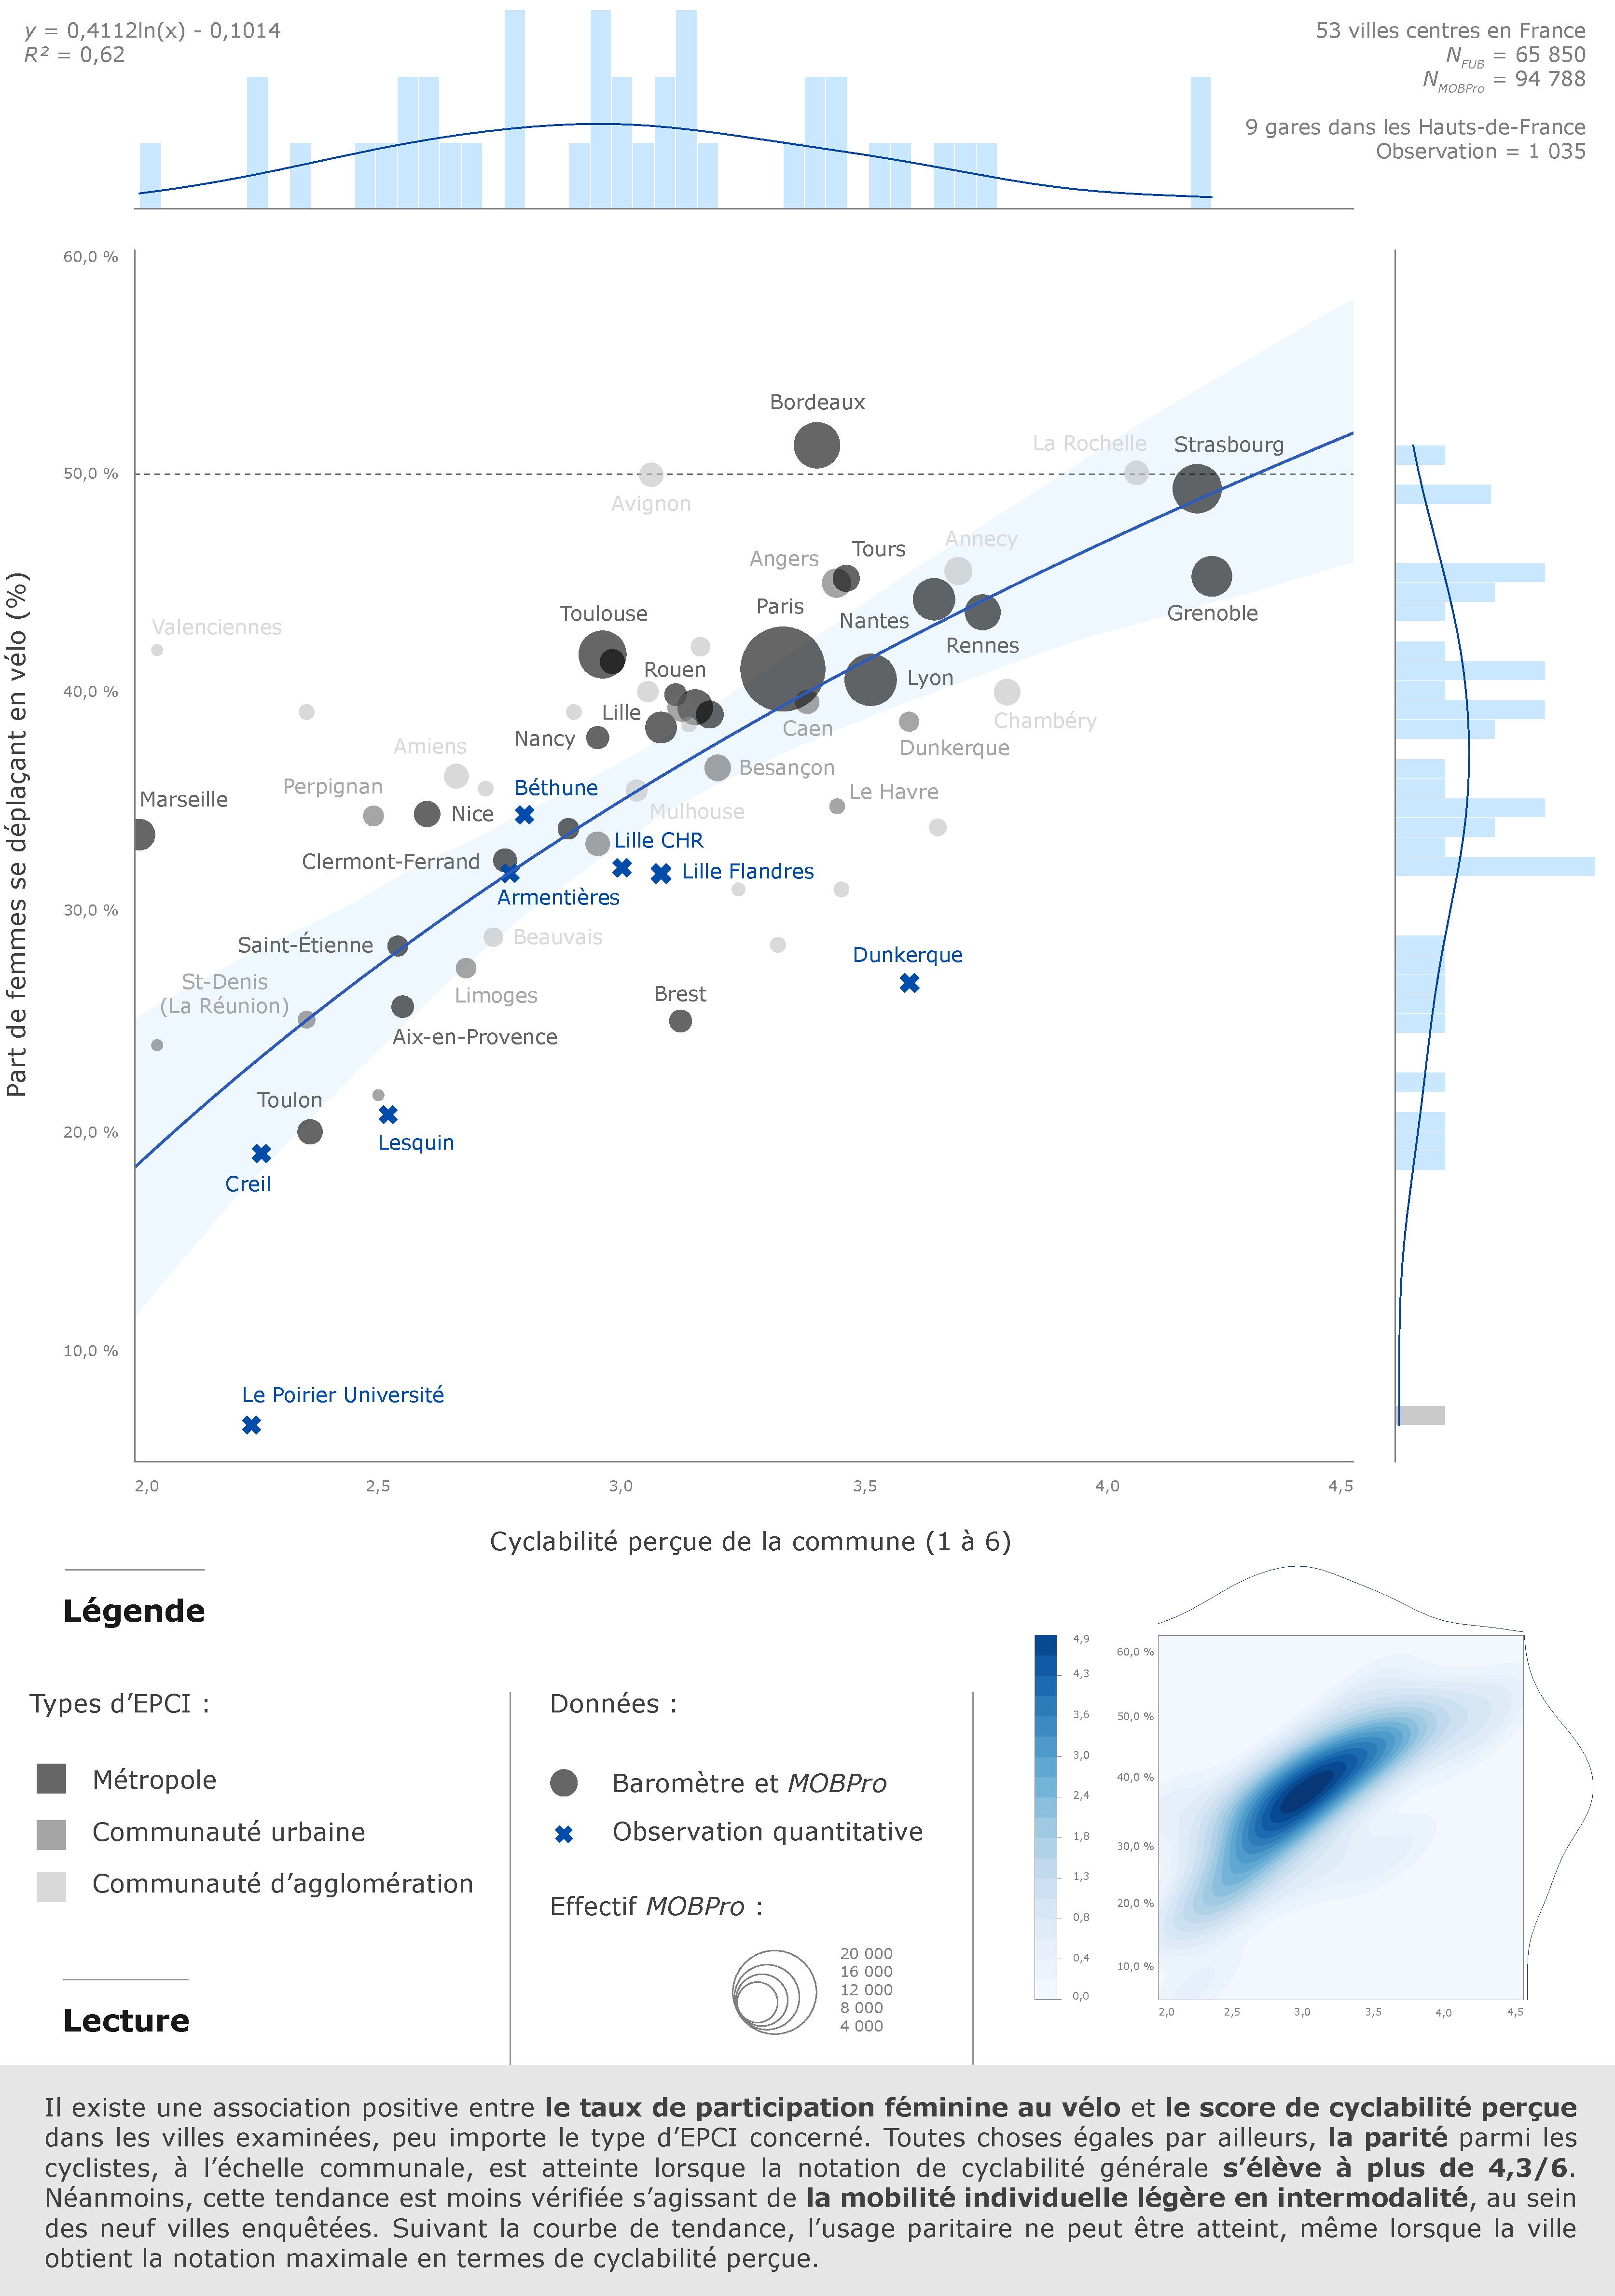
\includegraphics[width=1\columnwidth]{src/Figures/Chap-4/FR_Regression_genre_cyclabilite_OLS.pdf}}
        \vspace{5pt}
        \begin{flushright}\scriptsize{
        Jeux de données~: \textsl{Baromètre des Villes Cyclables} \textcolor{blue}{\autocite{fub_barometre_2021}} et \textsl{MOBPro} \textcolor{blue}{\autocite{insee_documentation_2023}}
        \\
        Auteur~: \textcolor{blue}{Dylan Moinse (2023)}
        %\\
        %Réalisation avec \Marque{Python}~et sur \Marque{Illustrator}
        }\end{flushright}
    \end{figure}

    %% Régression linéaire Observation quantitative
En prenant en considération l'observation quantitative des voyageur·se·s intermodaux·les optant pour le vélo ou des solutions de micro-mobilité dans la région, cette analyse statistique soutient la courbe de régression linéaire explorant l'usage genré du vélo en lien avec la cyclabilité, en particulier au sujet de la \acrshort{TEP} lorsqu'elle est associée avec le train. En guise d'illustration, citons le cas des usager·ère·s ayant recours à la trottinette électrique depuis la halte du Poirier Université, qui sont très rarement des femmes (5~\%, sur 19 observations) et qui font face à un score de cyclabilité de~2,24. Cette tendance se reflète également dans les gares de Lesquin (16~\%, sur 19 observations), Armentières (17~\% sur 58 observations) et Creil (19~\%, sur 54 observations), où les notes de cyclabilité varient de 2,26 à~2,77. \textsl{A contrario}, les disparités liées au genre sont moins accentuées aux gares de Lille Flandres (28~\%, sur 127 observations), Béthune (31~\%, sur 35 observations) et Lille CHR (32~\%, sur 57 observations), où la cyclabilité perçue est comprise entre~2,80 et~3,08.

    % Exception Dunkerque
Cependant, la gare de Dunkerque constitue une exception, caractérisée par une cyclabilité relativement élevée, mais marquée par une utilisation du vélo et de la micro-mobilité encore dominée par les usagers masculins (29~\%, sur 91 observations). Ce phénomène pourrait être lié aux effets des politiques de transport public gratuit depuis 2018 \textcolor{blue}{\autocite{heran_transports_2020}}\index{Héran, Frédéric|pagebf} dont les effets sur les pratiques genrées restent à étudier\footnote{
    Plus généralement, des discussions continuent d'alimenter la communauté scientifique et opérationnelle en ce qui concerne les relations entre les politiques de gratuité du transport public et l'usage du vélo. À Dunkerque, \textcolor{blue}{Claire-Marine} \textcolor{blue}{\textcite[89]{javary_gratuite_2020}}\index{Javary, Claire-Marine|pagebf}\index{Delevoye, Vanessa|pagebf}\index{Hasiak, Sophie|pagebf}\index{Huré, Maxime|pagebf} suggère qu'il n'existe pas d'effet de substitution modale du vélo et propose de dépasser ce débat pour entrevoir un système intermodal qui positionne ces modes de déplacement comme des alliés de la transition mobilitaire.
}. En comparaison avec l'utilisation exclusive du vélo classique, un second résultat qui émerge est néanmoins la réduction de la représentation des femmes parmi les utilisateur·rice·s de la micro-mobilité intermodale au sein de la même ville (voir l'\hyperref[fig-chap4:regression-genre-cyclabilite]{illustration~\ref{fig-chap4:regression-genre-cyclabilite}}, page~\pageref{fig-chap4:regression-genre-cyclabilite}). Cette observation souligne qu'un score de cyclabilité de~4,3/6 ne serait pas suffisant pour atteindre la parité parmi les voyageur·se·s ferroviaires qui optent pour la mobilité individuelle légère. Il faudrait effectivement une notation supérieure à la valeur maximale possible, soit six points, pour que la courbe puisse atteindre un seuil paritaire. Cette tendance suggère dès lors que l'amélioration de la cyclabilité des territoires à elle-seule ne suffirait pas à corriger les inégalités de genre observées concernant l'usage intermodal de la micro-mobilité.%%Rédigé%%

   %% Figure régression linéaire cyclabilité et genre
    \begin{figure}[h!]\vspace*{4pt}
        \caption{Modèle de régression linéaire entre la répartition genrée du vélo et les questions exploitées pour agréger le score de cyclabilité perçue.}
        \label{fig-chap4:regression-genre-cyclabilite-questions-detailees}
        \centerline{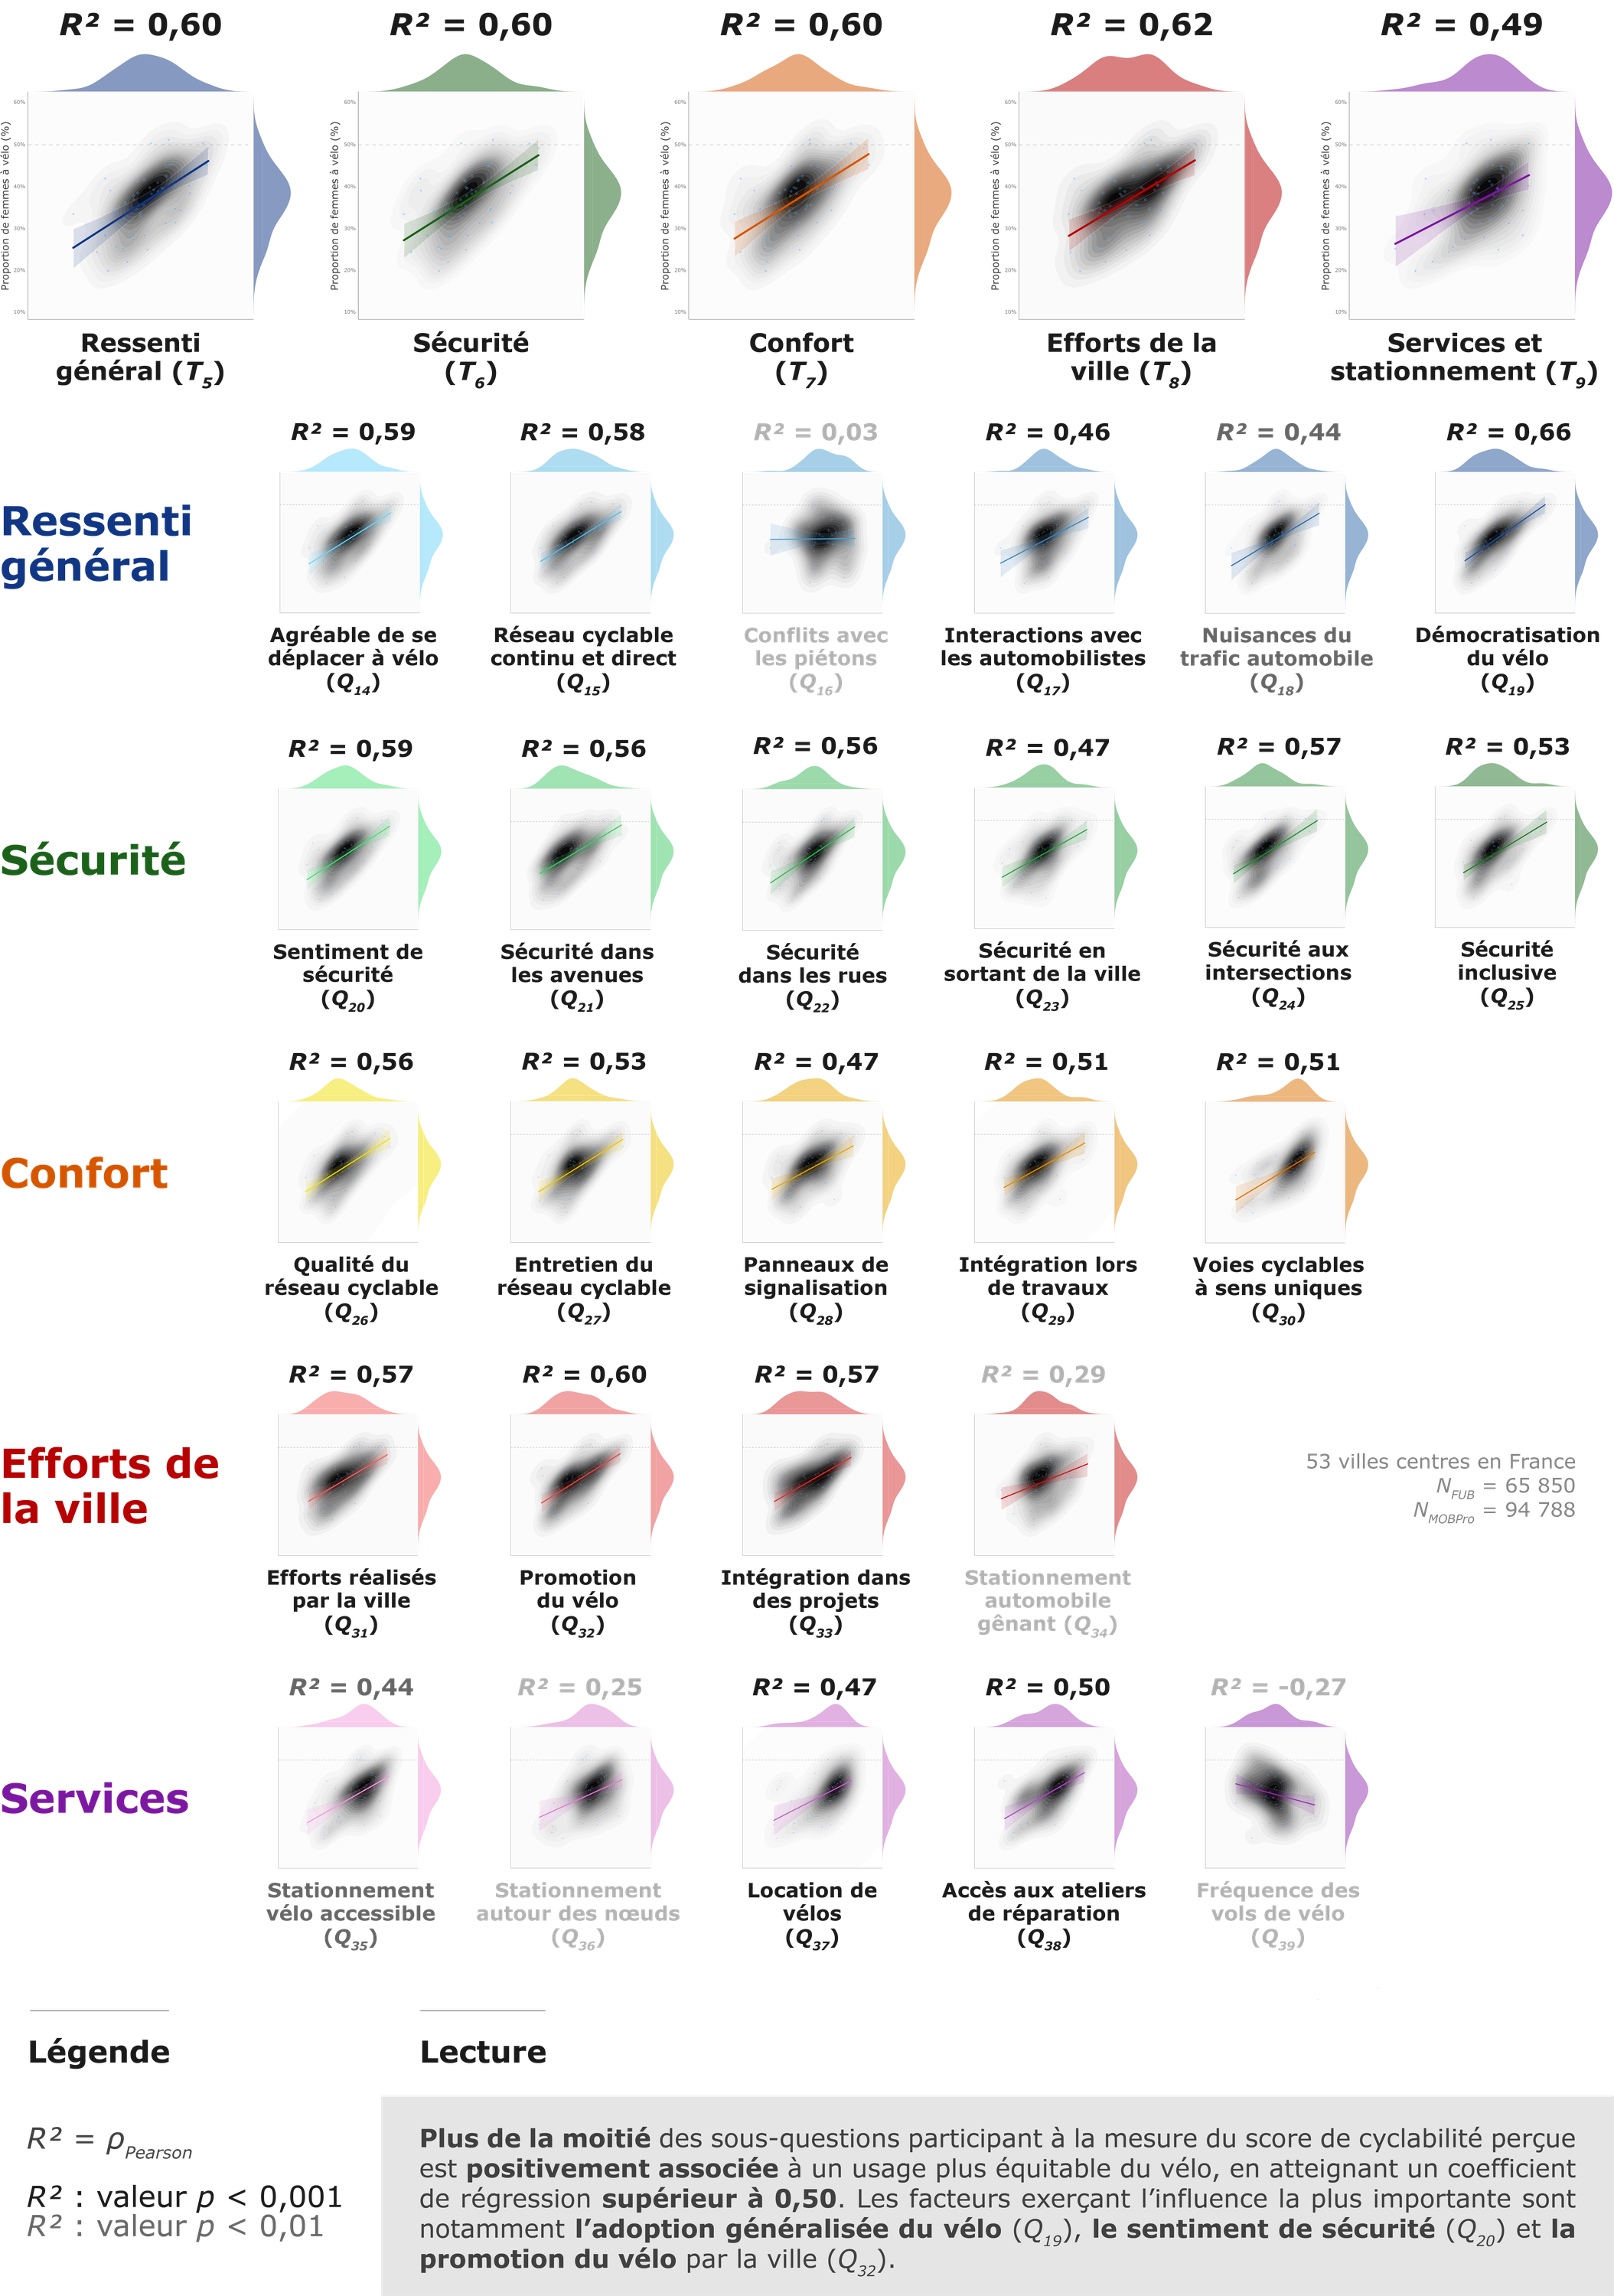
\includegraphics[width=1\columnwidth]{src/Figures/Chap-4/FR_Regression_sous_facteurs_OLS.png}}
        \vspace{5pt}
        \begin{flushright}\scriptsize{
        Jeux de données~: \textsl{Baromètre des Villes Cyclables} \textcolor{blue}{\autocite{fub_barometre_2021}} et \textsl{MOBPro} \textcolor{blue}{\autocite{insee_documentation_2023}}
        \\
        Auteur~: \textcolor{blue}{Dylan Moinse (2023)}
        }\end{flushright}
    \end{figure}

    %% Catégories liées à la cyclabilité
Une fois le lien établi entre les problématiques liées à la cyclabilité perçue et à l'usage inégalitaire de la mobilité individuelle légère au prisme du genre, l'analyse statistique a été affinée pour discerner les sous-facteurs exerçant un certain poids dans cette association positive. L'objectif de cette investigation est d'offrir une perspective qualitative sur la cyclabilité. En réexaminant les cinq thèmes définis dans le cadre du questionnaire conduit par la \textcolor{blue}{\textcite{fub_barometre_2021}}\index{FUB@\textsl{FUB}|pagebf}, il est possible de déterminer l'influence de chaque dimension évaluée par les usager·ère·s du vélo, en conservant les interrelations entre la cyclabilité et le taux de représentation des femmes à vélo. Le premier thème du questionnaire portant sur le \Guillemets{ressenti général} (\(T_{5}\)) de l'environnement cyclable montre une association significativement positive avec l'usage genré du vélo ($\hat{\beta}_{5}$~=~0,96,~$p$~\textless~0,06), révélant une influence nettement plus marquée que celle de la présence d'infrastructures cyclables ou de la démocratisation du vélo dans les zones urbaines. De plus, le score des \Guillemets{efforts de la ville} (\(T_{8}\)) contribue significativement à promouvoir une utilisation plus équitable du vélo ($\hat{\beta}_{8}$~=~0,58,~$p$~\textless~0,05). En revanche, l'indicateur lié au \Guillemets{confort} (\(T_{7}\)) à vélo présente une association négative ($\hat{\beta}_{7}$~=~-0,65,~$p$~\textless~0,08). En contraste, les thèmes relatifs à la \Guillemets{sécurité} (\(T_{6}\)) et aux \Guillemets{services et au stationnement} (\(T_{9}\)) ne montrent pas d'association significative ($\hat{\beta}_{6}$~=~-0,75 et $\hat{\beta}_{9}$~=~-0,22,~$p$~\texttt{>}~0,10). De même, au niveau des sous-questions incluses dans le questionnaire sur la cyclabilité perçue en France, aucune association significative n'est dérivée de la régression multivariée.%%Rédigé%%

    % Influence
Les résultats de la régression \acrshort{OLS} offrent un éclairage sur les relations entre divers indicateurs indépendants et l'usage genré du vélo, à l'échelle nationale. Les données ayant été normalisées, l'écart-type constitue l'unité de mesure. Par conséquent, les coefficients $\hat{\beta}_{i}$ indiquent dans quelle mesure la participation féminine au vélo fluctue en réponse aux variations de chaque indicateur indépendant, toutes choses égales par ailleurs~:
\begin{customitemize}
    \item Une augmentation d'un écart-type du score de \Guillemets{ressenti général} (\(T_{5}\), cyclabilité perçue) est associée à une augmentation de 0,959 fois l'écart-type de la variable dépendante~;
    \item Une augmentation d'un écart-type de la proportion d'itinéraires cyclables sur le réseau viaire (\(T_{3}\), cyclabilité objective) est associée à une augmentation de 0,595 fois l'écart-type de la variable dépendante~;
    \item Une augmentation d'un écart-type du score des \Guillemets{efforts de la ville} (\(T_{8}\), cyclabilité perçue) est associée à une augmentation de 0,578 fois l'écart-type de la variable dépendante~;
    \item Une augmentation d'un écart-type de la part modale du vélo (\(T_{1}\), sécurité par le nombre) est associée à une augmentation de 0,368 fois l'écart-type de la variable dépendante.
\end{customitemize}%%Rédigé%%

    %% Sous-questions sur la cyclabilité
En étudiant en détail chaque question, une série de régressions linéaires de type \textsl{Pearson} \textcolor{blue}{\autocite{pearson_vii_1896}}\index{Pearson, Karl|pagebf}\index{Henrici, Olaus Magnus Friedrich Erdmann|pagebf} révèle quant à elle une corrélation relativement significative dans l'ensemble, avec un coefficient de détermination ($R^2$) dépassant 0,50 pour plus de la moitié des questions, telle que démontrée par l'\hyperref[fig-chap4:regression-genre-cyclabilite-questions-detailees]{illustration~\ref{fig-chap4:regression-genre-cyclabilite-questions-detailees}} (page~\pageref{fig-chap4:regression-genre-cyclabilite-questions-detailees}). Ce sont notamment les facteurs suivants qui exercent une influence conséquente~:
    \begin{customitemize}
\item L'adoption généralisée du vélo (\(Q_{19}\),~$R^2$~=~0,66)~;
\item Le sentiment de sécurité ressenti à vélo (\(Q_{20}\),~$R^2$~=~0,60)~;
\item Le sentiment de sécurité en parcourant les rues résidentielles (\(Q_{22}\),~$R^2$~=~0,60)~;
\item La promotion du vélo par la ville (\(Q_{32}\),~$R^2$~=~0,60)~;
\item L'aspect ludique et agréable du vélo en ville (\(Q_{14}\),~$R^2$~=~0,59)~;
\item La capacité à se déplacer rapidement et directement à travers le réseau cyclable (\(Q_{15}\),~$R^2$~=~0,58)~;
\item L'expérience de sécurité lors de la traversée des intersections (\(Q_{24}\),~$R^2$~=~0,57)~;
\item L'implication des cyclistes dans les projets sur la mobilité et le développement urbain (\(Q_{33}\),~$R^2$~=~0,57)~;
\item Les efforts municipaux visant à renforcer le développement du vélo (\(Q_{31}\),~$R^2$~=~0,57)~;
\item La qualité du réseau cyclable (\(Q_{26}\),~$R^2$~=~0,56)~;
\item Le sentiment de sécurité sur les voies principales (\(Q_{21}\),~$R^2$~=~0,56).
    \end{customitemize}
Seules deux questions ne contribuent pas à la relation entre la cyclabilité et la répartition genrée du vélo~: celles liées aux conflits avec les piéton·ne·s (\(Q_{16}\),~$R^2$~=~0,03) et à la fréquence des vols de vélos (\(Q_{39}\),~$R^2$~=~-0,27).%%Rédigé%%

    %% Synthèse sous-questions
Il ressort que de multiples facteurs jouent un rôle crucial dans la notion de cyclabilité en tant que variable explicative en faveur d'un développement plus inclusif de la mobilité individuelle légère en France. La démocratisation du vélo, associée à sa visibilité, émerge comme une sous-variable essentielle dans cette équation, tout comme les considérations relatives au sentiment de sécurité des cyclistes, la mise en place d'un réseau cyclable continu et direct dans les zones résidentielles ainsi que les rues à double sens cyclable qui jouent un rôle fondamental en faveur d'une expérience considérée comme positive. De plus, les politiques cyclables sous l'impulsion de la ville revêtent une importance égale aux côtés de stratégies de communication efficaces et de concertations de projets urbains faisant participer les cyclistes. En parallèle, il paraît primordial de ne pas sous-estimer les facteurs contribuant à l'amélioration de la cyclabilité au sein des municipalités, notamment le sentiment de sécurité sur les voies principales, aux intersections et aux carrefours giratoires, le développement d'infrastructures sécurisées adaptées aux besoins des populations les plus vulnérables, l'entretien du réseau cyclable et un accès pratique aux services de réparation de vélos (voir l'\hyperref[fig-chap4:regression-genre-cyclabilite-questions-detailees]{illustration~\ref{fig-chap4:regression-genre-cyclabilite-questions-detailees}}, page~\pageref{fig-chap4:regression-genre-cyclabilite-questions-detailees}).%%Rédigé%%

    %% Parcours commentés 1
Dans le cadre de cette section, nous avons interrogé la perception de ces divers éléments qui influencent la qualité de la cyclabilité dans les territoires. Le témoignage de la participante \(PCTE_{1}\) offre un aperçu riche et détaillé de ces aspects. Cette dernière partage sa vision d'un environnement urbain au sein duquel \Guillemets{\textsl{l'aspect} [lié à la] \textsl{sécurité avec des pistes et des bandes cyclables} [et] \textsl{la ville agréable aussi} [\dots] \textsl{une ville apaisée, sans trop de voitures}}~[20:17, \(PCTE^{TC}_{1}\)] sont autant de facteurs priorisés. Le \Guillemets{sentiment de sécurité} (\(Q_{20}\)) est abordé par la participante qui évoque notamment les \Guillemets{interactions} (\(Q_{17}\)) et les \Guillemets{nuisances} (\(Q_{18}\)) liées au trafic automobile en matière de volume et de vitesse, en relatant qu'\Guillemets{\textsl{avec la route en pente, les voitures vont bien plus vite que} [sa] \textsl{trottinette\dots~Et} [qu'elle ne sent pas] \textsl{en sécurité sur cette partie du chemin. On est mélangé avec elles, et} [elle se] \textsl{retrouve coincée entre les voitures qui circulent et celles qui sont garées}}~[\(PCTE^{A}_{1}\)]. Ces situations de vulnérabilité génèrent un sentiment d'inconfort et d'impuissance, venant dégrader le \Guillemets{plaisir} de se déplacer à vélo ou en micro-mobilité (\(Q_{14}\)), comme l'explique la participante~: \Guillemets{\textsl{ce qui est, pas stressant, mais on va dire\dots un peu plus embêtant} [\dots] \textsl{il y a \textsl{beaucoup} de voitures et donc\dots étant donné que ma trottinette roule à 25 km/h maximum, j’ai peur d’embêter les voitures. Du coup, je me positionne sur le côté de la chaussée et j’essaie d’accélérer au max.}}~[00:27, \(PCTE^{TC}_{1}\)].%%Rédigé%%

    %% Figure 2 PCTE1E Maubeuge
    \begin{figure}[h!]\vspace*{4pt}
        \caption{Image extraite de l'itinéraire filmé en rabattement vers la gare Lille Flandres et illustrant la manœuvre d'évitement d'un stationnement obstructif (\(PCTE^{A}_{1}\)).}
        \label{fig-chap4:pcte1a-stationnement-genant}
        \centerline{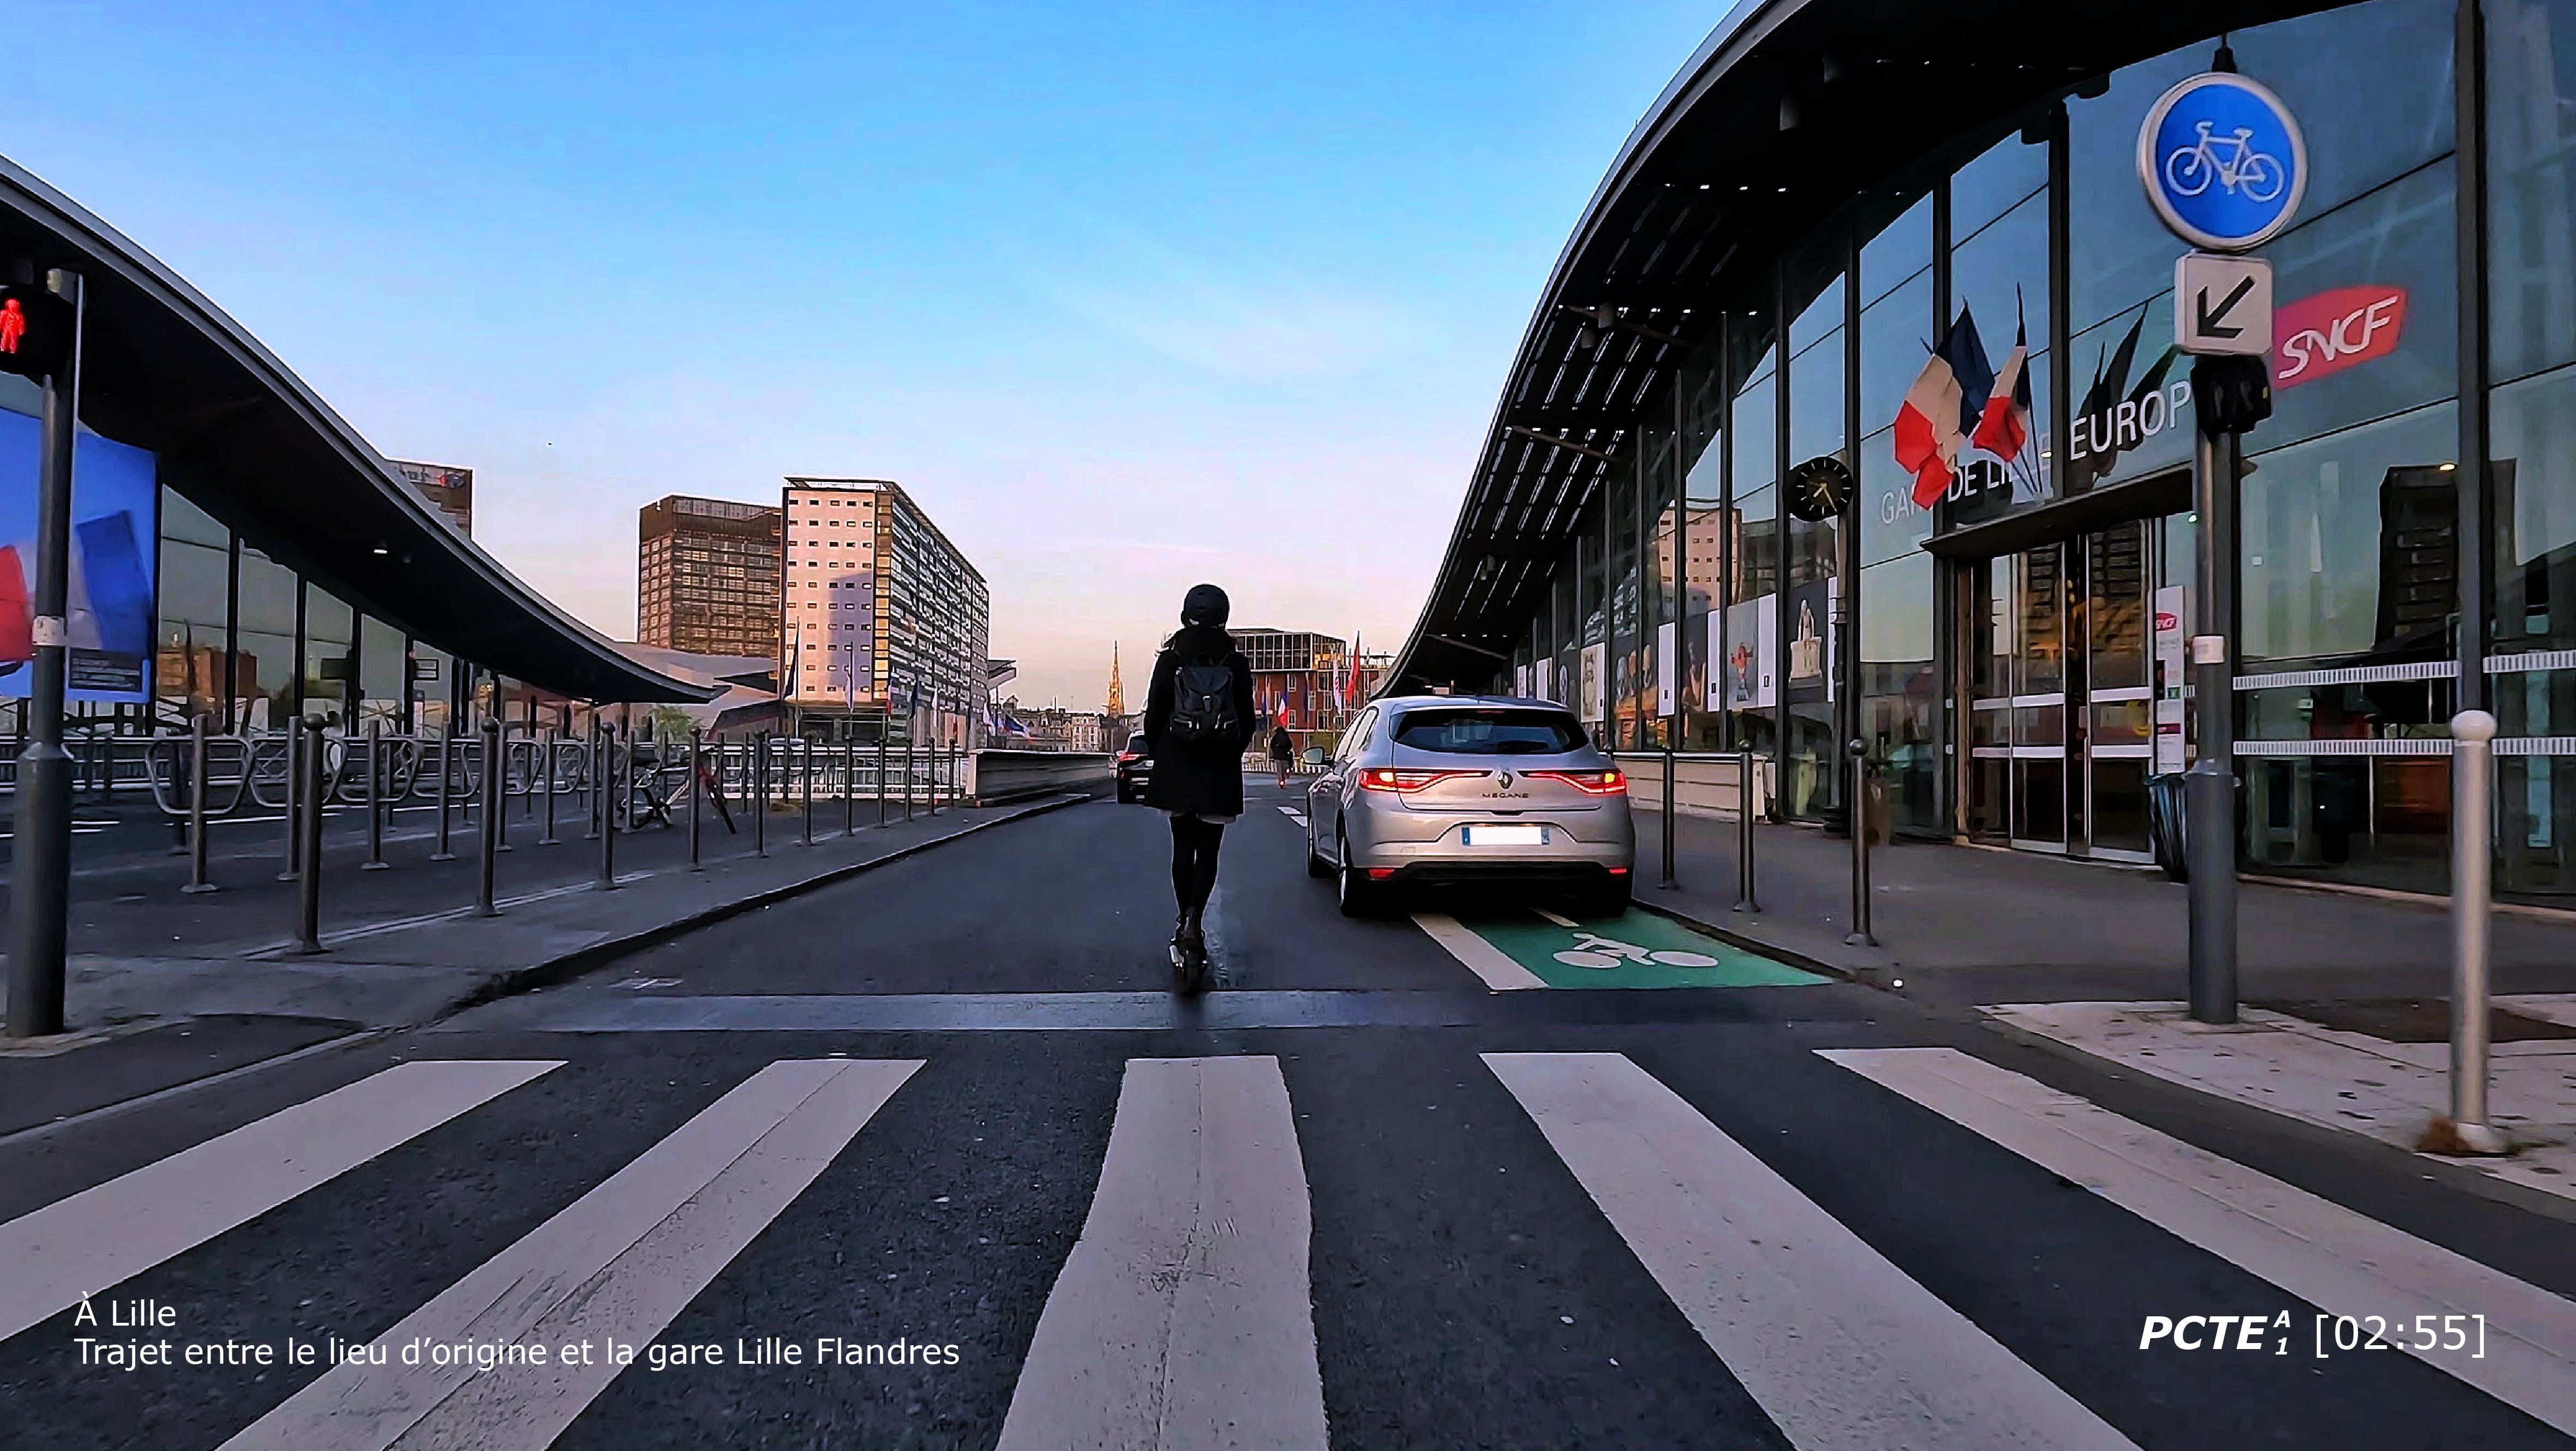
\includegraphics[width=1\columnwidth]{src/Figures/Chap-4/Extrait_Video_PCTE1_Access_8.jpg}}
        \vspace{5pt}
        \begin{flushright}\scriptsize{
        Auteur~: \textcolor{blue}{Dylan Moinse (2022)}
        }\end{flushright}
    \end{figure}

    %% Parcours commentés 2
La gestion des intersections est également un point critique, bien plus décrit par la participante du \(PCTE_{1}\) que le participant du \(PCTE_{2}\). Le traitement des \Guillemets{intersections} (\(Q_{24}\)) intervient dans les difficultés rencontrées dans la pratique cyclable, à l'instar du \Guillemets{\textsl{gros point noir} [qui] \textsl{est le rond-point} [\dots] [où la participante a] \textsl{peur quand} [elle est] \textsl{dans le rond-point, car} [elle ne peut] \textsl{pas trop} [se] \textsl{retourner pour voir ce qu’il se passe derrière étant donné} [qu'elle est] \textsl{moins stable sur une trottinette que sur un vélo}}~[03:04, \(PCTE^{TC}_{1}\)]. Par ailleurs, la \Guillemets{qualité du réseau cyclable} (\(Q_{26}\)) est un facteur déterminant pour une circulation sécurisée en mobilité individuelle légère. La participante exprime une préférence pour les voies réservées aux bus, qu'elle trouve \Guillemets{\textsl{agréables}}, car elle peut \Guillemets{\textsl{circuler assez facilement}} [00:27, \(PCTE^{TC}_{1}\)] et \Guillemets{car c'est beaucoup plus sécurisant, car c'est plus large} [02:16, \(PCTE^{TC}_{1}\)], aussi bien à Lille qu'à Maubeuge. Elle aborde cependant avec moins d'enthousiasme les bandes cyclables, évoquant des situations dans lesquelles elle se sent contrainte d'éviter certains tronçons en raison de l'inattention des automobilistes, étant \Guillemets{\textsl{sur le côté}} [00:27, \(PCTE^{TC}_{1}\)] tandis que les \Guillemets{\textsl{voitures ne} [font] \textsl{pas attention}} [03:04, \(PCTE^{TC}_{1}\)] (voir l'\hyperref[fig-chap4:pcte1a-stationnement-genant]{extrait vidéo~\ref{fig-chap4:pcte1a-stationnement-genant}}, page~\pageref{fig-chap4:pcte1a-stationnement-genant}). Enfin, le parcours commenté réalisé avec l'usagère en \acrshort{TEP} apporte un dernier enseignement sur l'importance de la \Guillemets{signalétique} (\(Q_{28}\)) et de la \Guillemets{communication et de la promotion du vélo} (\(Q_{32}\)) par les autorités publiques. Un réseau cyclable bien conçu et clairement indiqué est essentiel pour éviter les confusions et les conflits d'usage entre cyclistes et automobilistes. La participante pointe du doigt les lacunes dans ces domaines, notamment le manque de visibilité et d'informations claires, le réseau \Guillemets{[manquant] \textsl{de couleurs} [\dots] \textsl{et d'informations}}~[\(PCTE^{E}_{1}\)] (voir l'\hyperref[fig-chap4:pcte1e-voie-bus]{extrait vidéo~\ref{fig-chap4:pcte1e-voie-bus}}, page~\pageref{fig-chap4:pcte1e-voie-bus}).%%Rédigé%%

    %% Figure 3 PCTE1E Maubeuge
    \begin{figure}[h!]\vspace*{4pt}
        \caption{Image extraite de l'itinéraire filmé en diffusion depuis la gare de Maubeuge révélant une voie bus dépourvue de marquage au sol discernable (\(PCTE^{E}_{1}\)).}
        \label{fig-chap4:pcte1e-voie-bus}
        \centerline{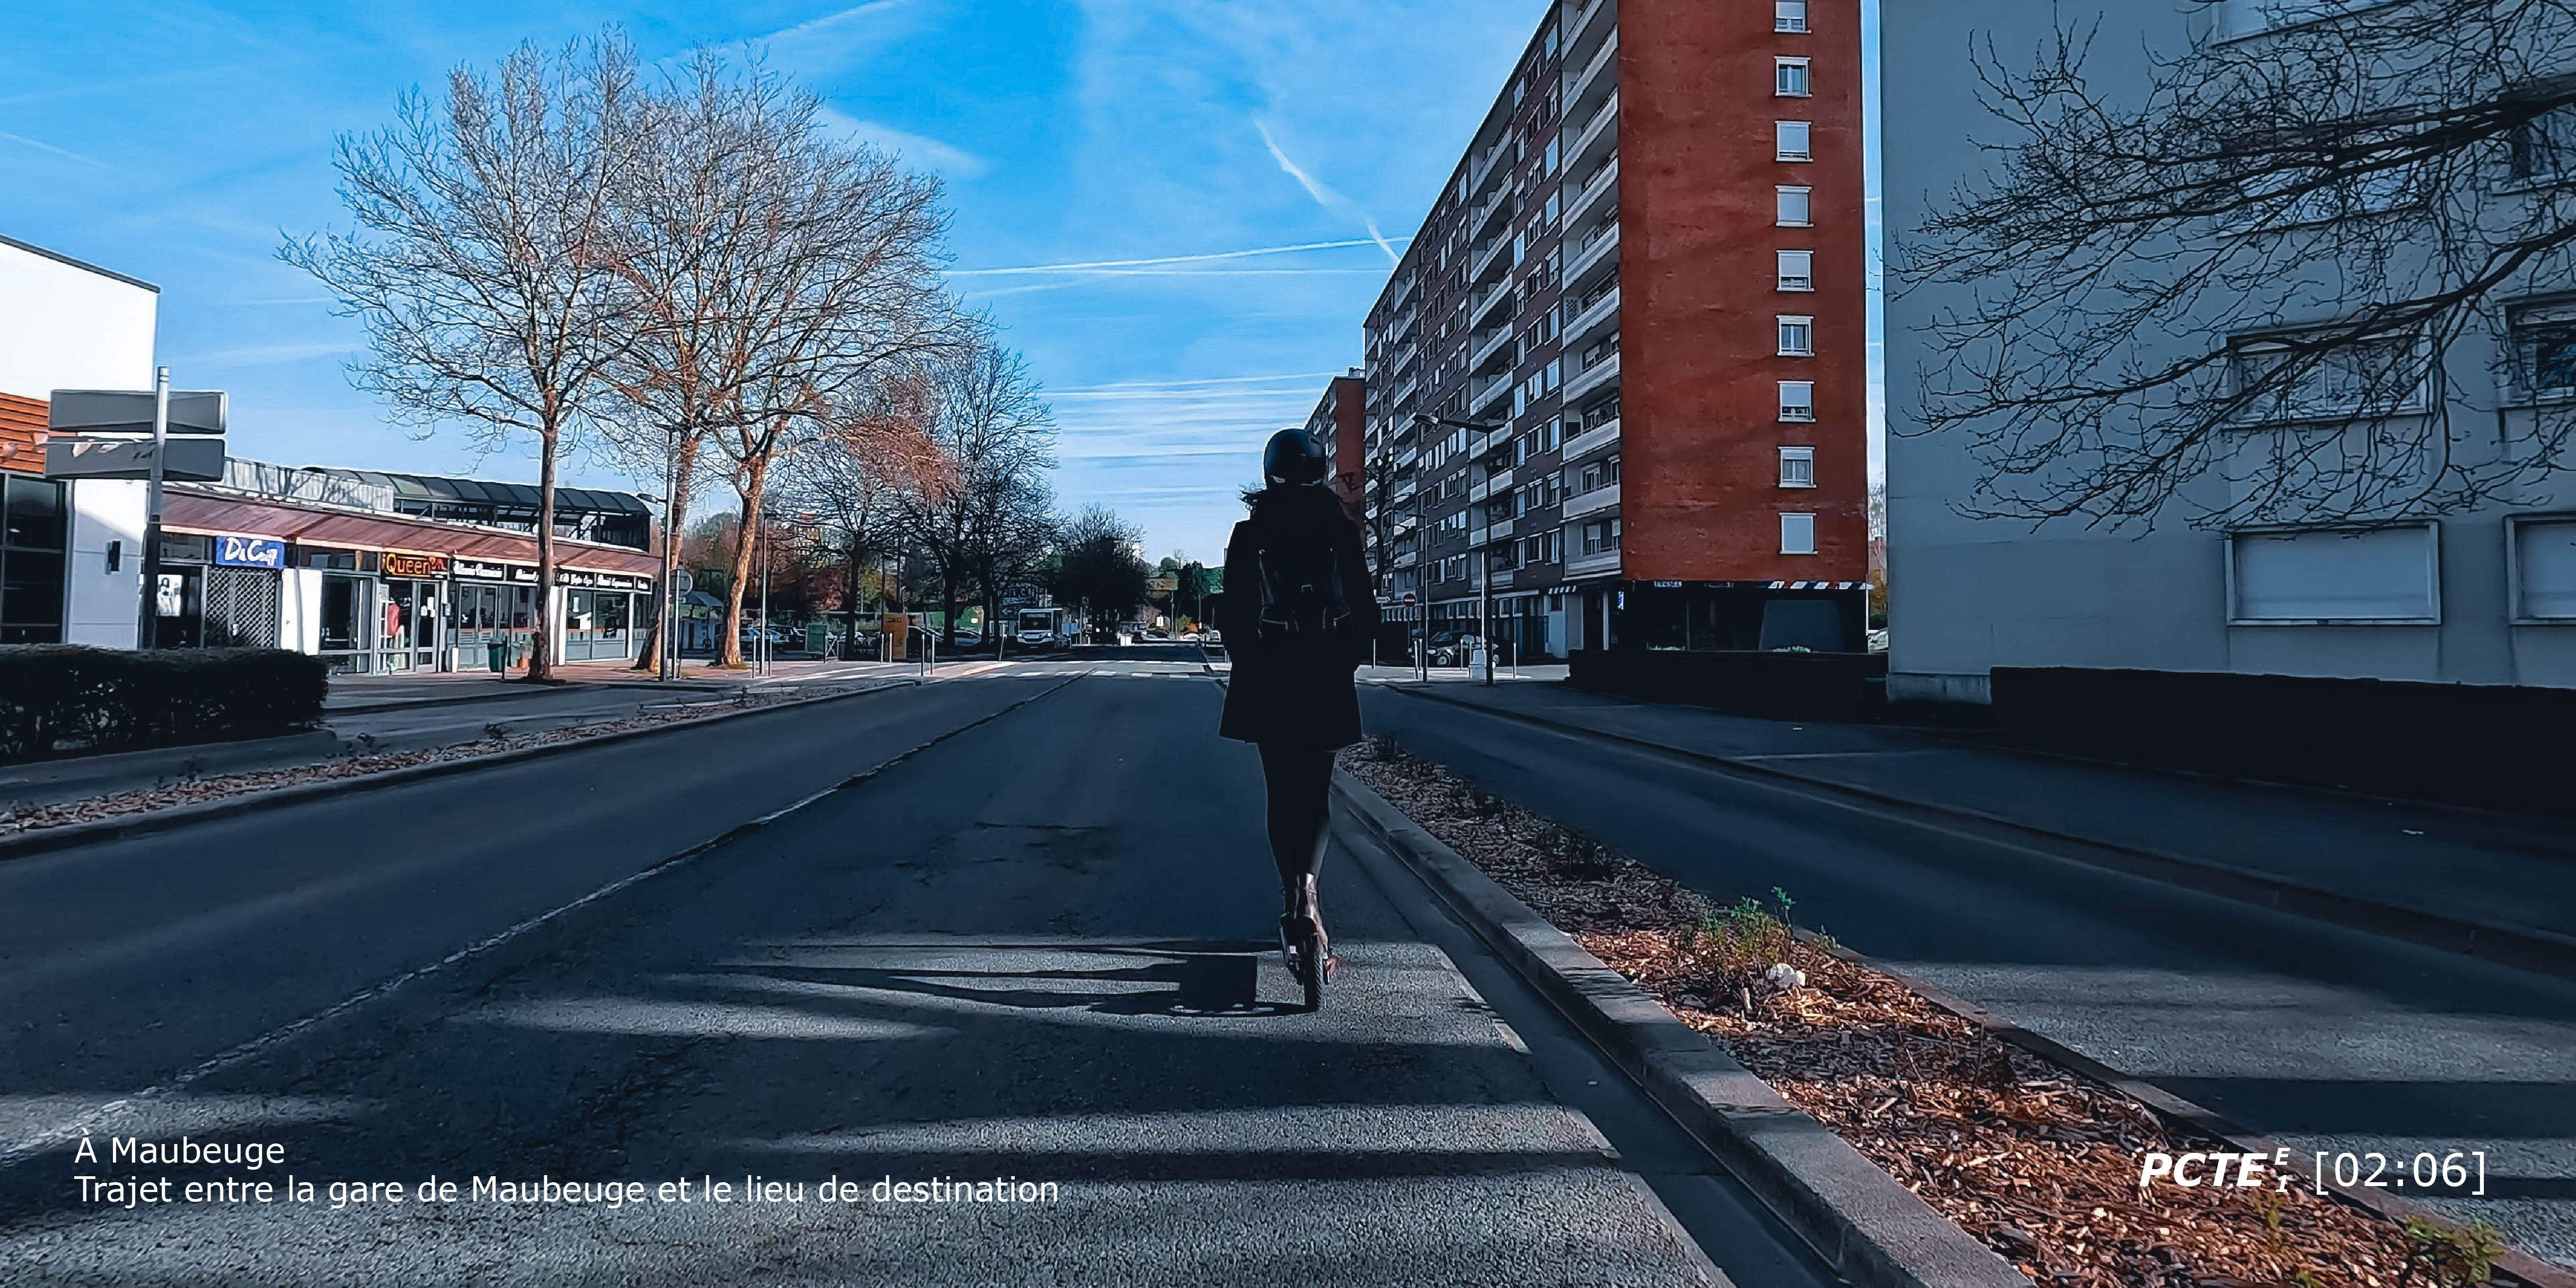
\includegraphics[width=1\columnwidth]{src/Figures/Chap-4/Extrait_Video_PCTE1_Egress_4.jpg}}
        \vspace{5pt}
        \begin{flushright}\scriptsize{
        Auteur~: \textcolor{blue}{Dylan Moinse (2022)}
        }\end{flushright}
    \end{figure}

    % 4.3.3.4.
    \needspace{1\baselineskip} % Réserve de l'espace
\subsubsection*{Photographie des villes françaises enquêtées selon la distribution genrée des cyclistes
    \label{chap4:comparaison-villes-fr-genre}
    }

    %% Classement des villes
Au moyen d'une analyse quantitative des jeux de données fournis par la \textcolor{blue}{\textcite{fub_barometre_2021}}\index{FUB@\textsl{FUB}|pagebf} et l'\textcolor{blue}{\textcite{insee_documentation_2023}}\index{Insee@\textsl{Insee}|pagebf}, cette sous-section vise à classifier les 53 villes françaises en fonction de leurs notations de cyclabilité et du degré de féminisation dans la pratique du vélo. Pour ce faire, la recherche a eu recours à une analyse bivariée\footnote{
    Une analyse bivariée est une méthode statistique qui examine la relation entre deux variables, en caractérisant la manière dont elles interagissent. Cela permet de comprendre s'il existe une corrélation ou une dépendance entre ces deux variables ainsi que la nature positive ou négative de cette relation. Une analyse bivariée peut donner lieu à la production d'une représentation graphique, telle une carte bivariée. Ce type de cartographie met alors en relief les deux variables conjointement, dans l'intérêt de montrer visuellement comment elles se comportent en relation l'une à l'autre.
} afin de mettre en exergue la corrélation positive observée sur le plan géographique. Quatre catégories émergent de cette analyse statistique~: (i) les villes tendant vers la parité et favorables au développement du vélo~; (ii) les villes favorables au développement du vélo, mais présentant des inégalités de genre~; (iii) les villes tendant vers la parité, mais défavorables au développement du vélo~; et (iv) les villes présentant des inégalités de genre et défavorables au vélo (voir la \hyperref[fig-chap4:carte-bivariee-genre-cyclabilite]{carte~\ref{fig-chap4:carte-bivariee-genre-cyclabilite}}, page~\pageref{fig-chap4:carte-bivariee-genre-cyclabilite}).%%Rédigé%%

   %% Figure carte bivariée cyclabilité et usage genré
    \begin{carte}[h!]\vspace*{4pt}
        \caption{Carte bivariée des 53 villes françaises examinées en fonction de la répartition genrée du vélo et de la cyclabilité perçue.}
        \label{fig-chap4:carte-bivariee-genre-cyclabilite}
        \centerline{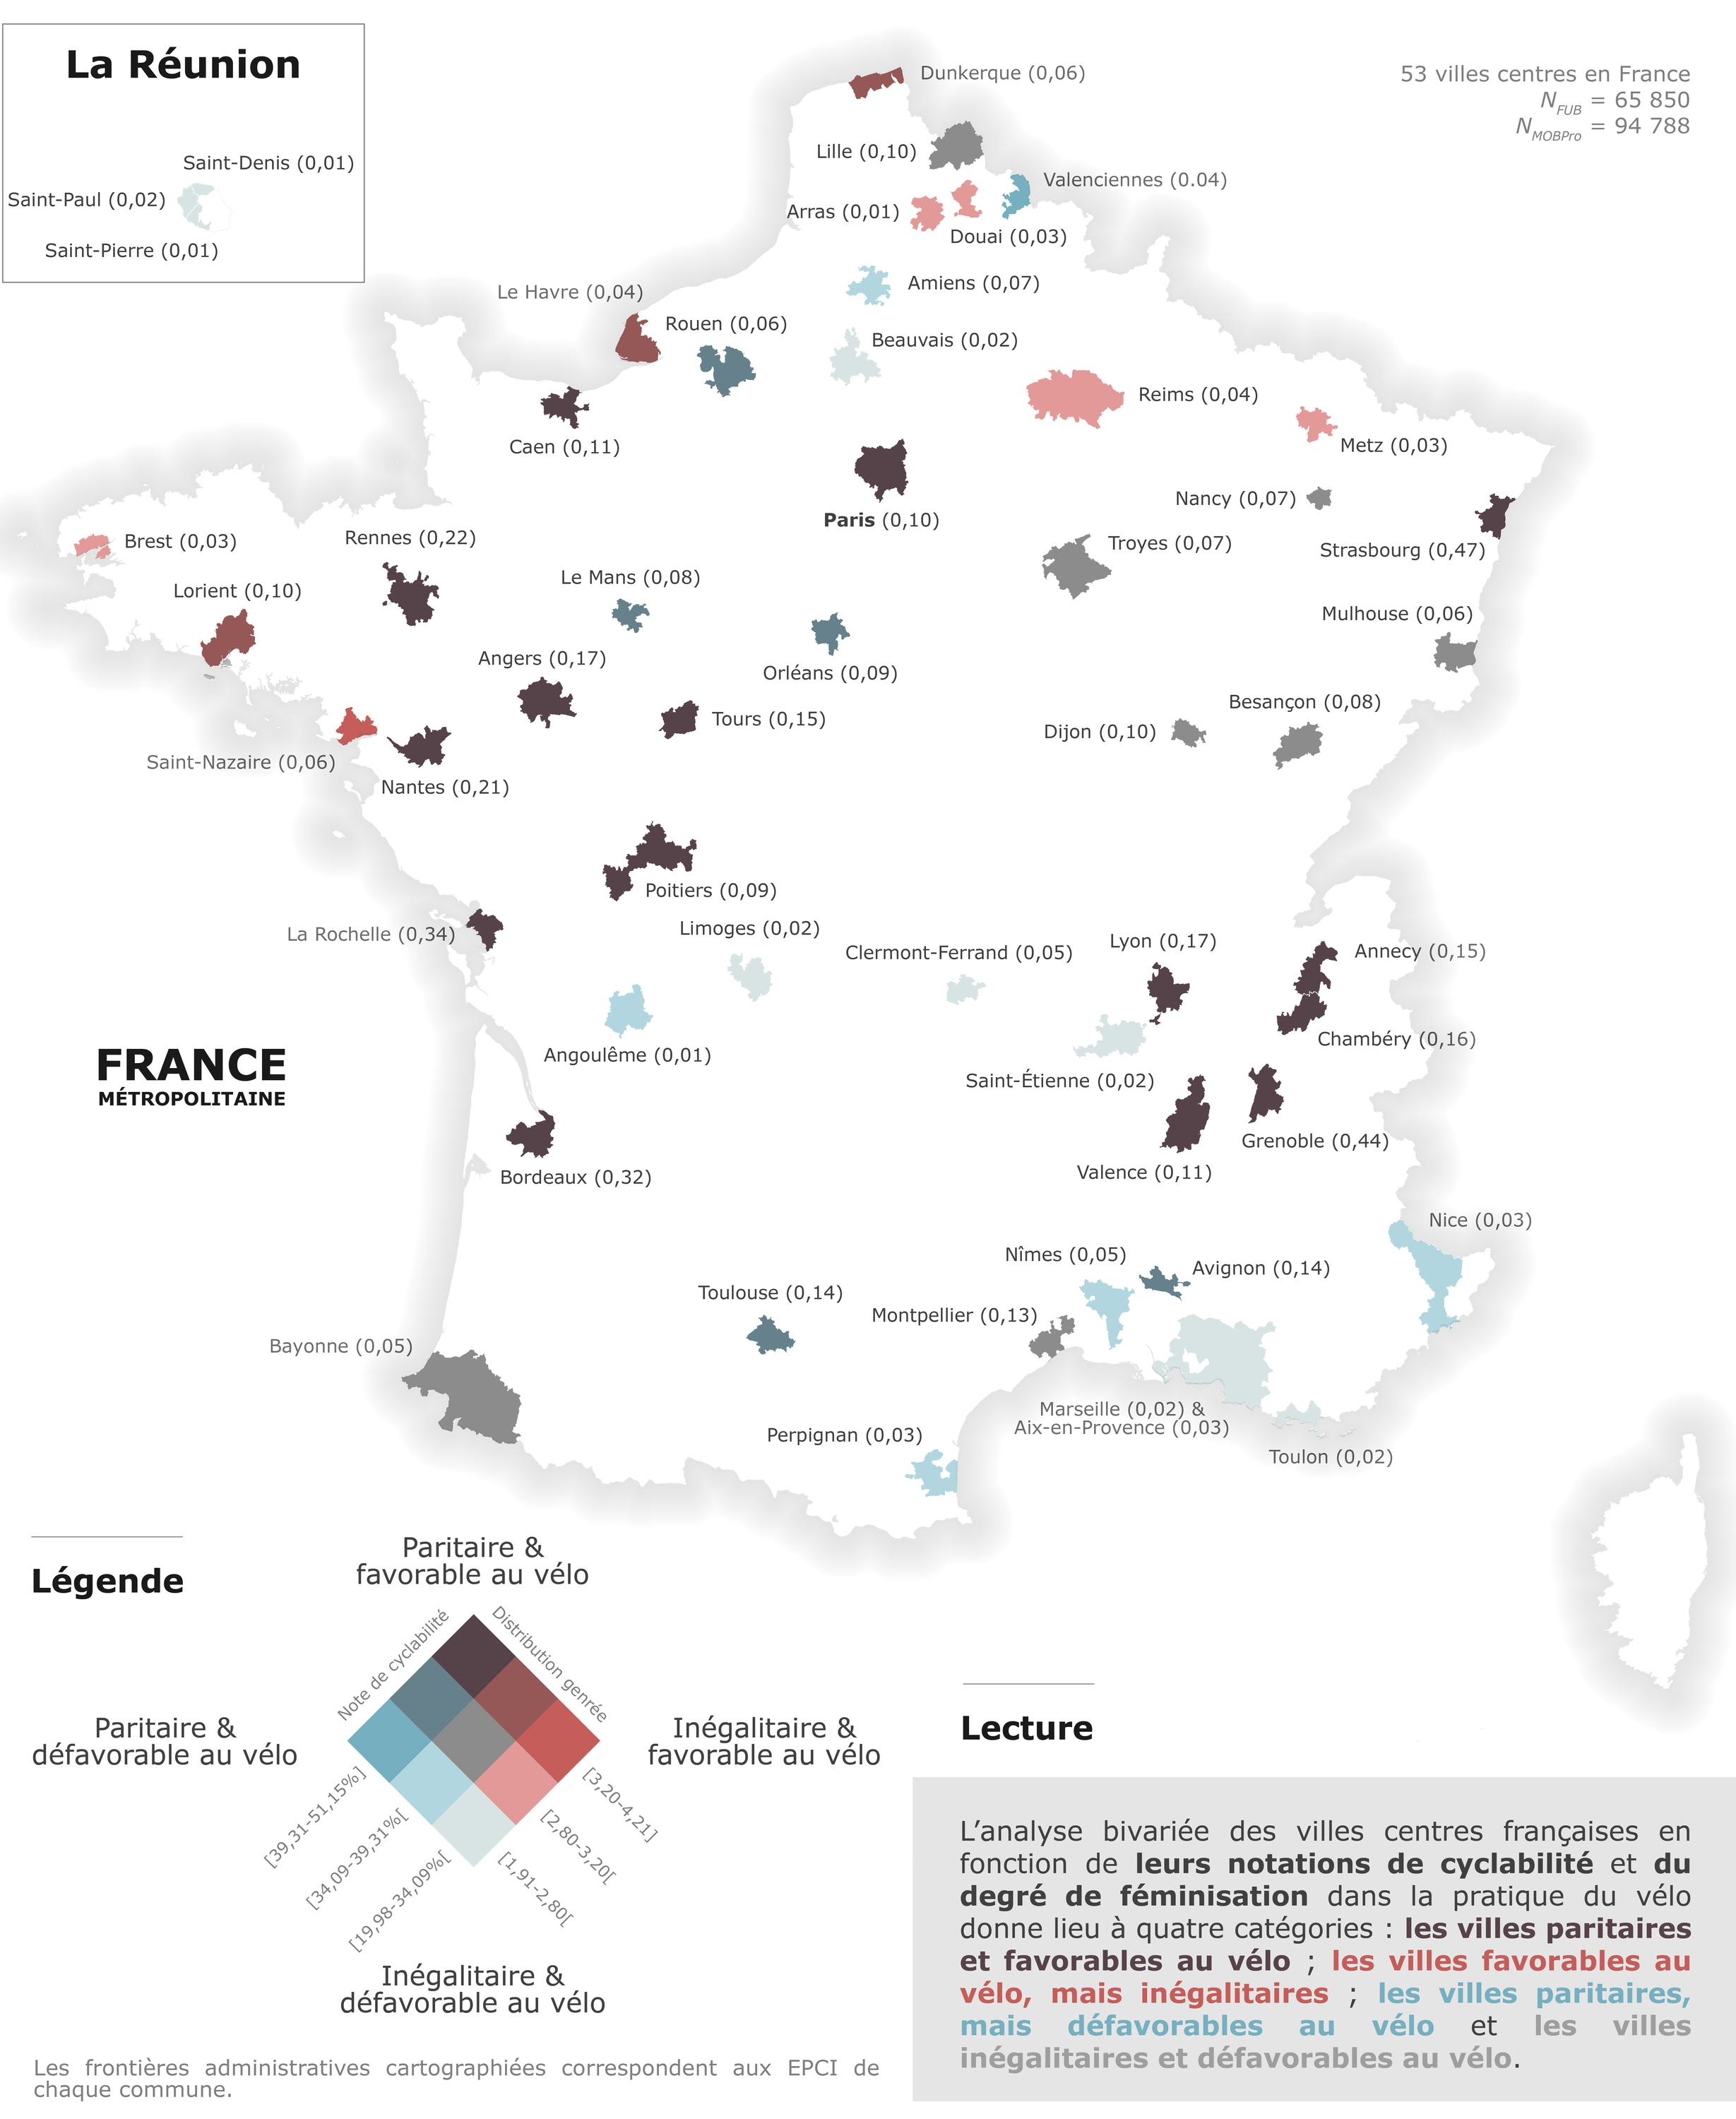
\includegraphics[width=1\columnwidth]{src/Figures/Chap-4/FR_Carte_bivariee_cyclabilite_genre_OLS.jpg}}
        \vspace{5pt}
        \begin{flushright}\scriptsize{
        Jeux de données~: \textsl{Baromètre des Villes Cyclables} \textcolor{blue}{\autocite{fub_barometre_2021}} et \textsl{MOBPro} \textcolor{blue}{\autocite{insee_documentation_2023}}
        \\
        Auteur~: \textcolor{blue}{Dylan Moinse (2023)}
        }\end{flushright}
    \end{carte}

    %% Description de la carte extrêmes
La \hyperref[fig-chap4:carte-bivariee-genre-cyclabilite]{carte~\ref{fig-chap4:carte-bivariee-genre-cyclabilite}} (page~\pageref{fig-chap4:carte-bivariee-genre-cyclabilite}) offre une représentation visuelle replaçant les villes en fonction de la distribution genrée du vélo et de la cyclabilité ressentie par les usager·ère·s, à partir d'intervalles réguliers. La typologie des cinquante-trois villes étudiées met en avant les villes caractérisées par un usage paritaire du vélo et une note de cyclabilité élevée. Ces villes se situent principalement dans l'ouest de la France métropolitaine, à l'exception de la Bretagne, incluant Bordeaux, Nantes, Rennes, Tours, Angers, Poitiers, ainsi que des villes à l'est du pays, telles que Strasbourg, Grenoble, Annecy, Chambéry et Lyon. À l'opposé, les villes recevant des évaluations plus basses pour les deux variables sont principalement situées dans le sud de la France métropolitaine, englobant des lieux tels que Toulon, Marseille, Aix-en-Provence, Saint-Étienne, Limoges et Clermont-Ferrand. C'est également le cas des villes du département de La Réunion, comme Saint-Pierre, Saint-Paul et Saint-Denis qui entrent dans cette catégorie.%%Rédigé%%

    %% Description de la carte nuances
De plus, plusieurs régions qui offrent des conditions favorables à la pratique du vélo, mais qui rencontrent des défis pour parvenir à une distribution genrée équilibrée du vélo, sont principalement situées dans le nord de la France métropolitaine, comprenant des villes comme Dunkerque, Le Havre, Arras, Douai et Reims, ainsi qu'en Bretagne, avec des exemples tels que Lorient, Brest et Saint-Nazaire. En revanche, certaines villes présentent une répartition genrée relativement équilibrée du vélo, mais maintiennent néanmoins des niveaux de cyclabilité relativement faibles. Cette dernière catégorie est illustrée par des villes telles qu'Amiens, Angoulême, Nice, Nîmes et Valenciennes.%%Rédigé%%

    % 4.3.3.5.
    \needspace{1\baselineskip} % Réserve de l'espace
\subsubsection*{Détermination d'un indicateur basé sur le développement inclusif du vélo et de la cyclabilité
    \label{chap4:definition-indicateur-genre}
    }

    %% Indicateur
À partir des trois variables examinées tout au long de cette sous-section, à savoir la répartition des femmes dans la pratique du vélo, la part modale du vélo et le score de cyclabilité d'une commune, le dernier objectif de cette recherche dédiée au genre et à la mobilité est d'introduire un indicateur qui englobe la cyclabilité et l'utilisation de la mobilité individuelle légère, en mettant particulièrement l'accent sur l'inclusion sociale de ces modes de déplacement. L'intérêt d'un tel indice est de développer un outil utile pour évaluer l'interaction entre ces trois aspects dans le contexte des villes françaises. Cet indicateur, désigné par~\(I_{gcb}\) (de 0 à 1), est le résultat d'une combinaison de trois indices~: un indice basé sur la répartition des femmes cyclistes (avec une valeur idéale fixée à 50~\%), noté ~\(I_{g}\)~; un deuxième indice évaluant le développement du vélo (avec une valeur idéale fixée à 25~\%), désigné par~\(I_{c}\)~; et un troisième indice basé sur l'évaluation de la cyclabilité attribuée par les utilisateur·rice·s, identifié sous le nom de~\(I_{b}\). Cet indicateur global est calculé d'après la \hyperref[equation-chap4:indice-equite]{formule~\ref{equation-chap4:indice-equite}} (page~\pageref{equation-chap4:indice-equite})~:%%Rédigé%%

    \begin{equation}
    \label{equation-chap4:indice-equite}
    \begin{aligned}
&I_{g} = \frac{Min(G_{fc}, 50~\%)}{50~\%}
    \\\\
&I_{c} = \frac{Min(C_{ms}, 25~\%)}{25~\%}
    \\\\
&I_{b} = \frac{B_{s}}{6}
    \\\\
&I_{gcb} = I_{g} * I_{c} * I_{b}
    \end{aligned}
    \end{equation}

    \begin{align*}
        &\text{où~:} \\
&G_{fc} \text{ représente la part des femmes se déplaçant à vélo~;} \\
&C_{ms} \text{ représente la part modale du vélo dans la commune~;} \\
&B_{s} \text{ représente l'indice de cyclabilité de la commune~;} \\
&I_{gcb} \text{ agrège }I_{g}\text{ ; }I_{c}\text{ ; et }I_{b}\text{.}
    \end{align*}

    %% Meilleurs scores de l'indicateur
Le développement de cet indicateur factorisant l'usage paritaire de la mobilité individuelle avec le développement de ces modes de déplacement légers et de la cyclabilité de la commune offre une compréhension enrichie du profil des villes étudiées. Avec un score moyen de 0,098 et une médiane de 0,067, les cinquante-trois villes centres sont encore loin d'atteindre un système de mobilité alternatif pouvant être considéré comme durable et inclusif, tant en termes d'urbanisme, de services que de démographie. Il est à noter que les quatre villes qui se démarquent de ce classement sont Strasbourg (\(I_{gcb}\)~=~0,47), Grenoble (\(I_{gcb}\)~=~0,44), La Rochelle (\(I_{gcb}\)~=~0,34) et Bordeaux (\(I_{gcb}\)~=~0,32), comme l'indique l'\hyperref[fig-chap4:carte-bivariee-genre-cyclabilite]{illustration~\ref{fig-chap4:carte-bivariee-genre-cyclabilite}} (page~\pageref{fig-chap4:carte-bivariee-genre-cyclabilite}).%%Rédigé%%

    %% Mauvais scores de l'indicateur
Parmi les villes incluses dans l'étude, 47 d'entre elles obtiennent des scores inférieurs à 0,2, tandis que celles situées en bas du classement incluent Saint-Pierre (\(I_{gcb}\)~=~0,011), Angoulême (\(I_{gcb}\)~=~0,012), Arras (\(I_{gcb}\)~=~0,012), Saint-Denis (\(I_{gcb}\)~=~0,013), Limoges (\(I_{gcb}\)~=~0,015), Marseille (\(I_{gcb}\)~=~0,015) et Saint-Étienne (\(I_{gcb}\)~=~0,015). Il est intéressant de mentionner la position des grandes métropoles françaises au travers de ce classement. Plus précisément, Rennes occupe la 5\textsuperscript{e} position (\(I_{gcb}\)~=~0,22), la 6\textsuperscript{e} pour Nantes (\(I_{gcb}\)~=~0,213), la 8\textsuperscript{e} pour Lyon (\(I_{gcb}\)~=~0,167), la 12\textsuperscript{e} pour Toulouse (\(I_{gcb}\)~=~0,144), la 14\textsuperscript{e} pour Montpellier (\(I_{gcb}\)~=~0,131), la 19\textsuperscript{e} pour Lille (\(I_{gcb}\)~=~0,100), la 20\textsuperscript{e} pour Paris (\(I_{gcb}\)~=~0,099) et la 30\textsuperscript{e} pour Rouen (\(I_{gcb}\)~=~0,061).%%Rédigé%%

    % 4.3.3.6.
    \needspace{1\baselineskip} % Réserve de l'espace
\subsubsection*{L'hospitalité territoriale vue au prisme de la cyclabilité et du genre
    \label{chap4:discussion-cyclabilite-genre}
    }

    % Littérature sur la cyclabilité et le genre
La présence d'une association positive entre l'utilisation inclusive du vélo et sa part modale au sein d'une agglomération, telle qu'elle a été validée dans la littérature scientifique existante \textcolor{blue}{\autocites[70]{goel_cycling_2022}[63]{garrard_revolutions_2006}}\index{Goel, Rahul|pagebf}\index{Goodman, Anna|pagebf}\index{Aldred, Rachel|pagebf}\index{Nakamura, Ryota|pagebf}\index{Tatah, Lambed|pagebf}\index{Garcia, Leandro Martin Totaro|pagebf}\index{Zapata-Diomedi, Belen|pagebf}\index{Sa, Thiago Herick de|pagebf}\index{Tiwari, Geetam|pagebf}\index{Nazelles, Audrey de|pagebf}\index{Tainio, Marko|pagebf}\index{Buehler, Ralph|pagebf}\index{Götschi, Thomas|pagebf}\index{Woodcock, James|pagebf}\index{Garrard, Jan|pagebf}, requiert une perspective renouvelée en prenant davantage en compte l'influence de l'environnement urbain et de l'expérience des cyclistes. Cette relation demeure effectivement indissociable de la cyclabilité des territoires \textcolor{blue}{\autocite{garrard_women_2021}}\index{Garrard, Jan|pagebf}\index{Buehler, Ralph|pagebf}\index{Pucher, John|pagebf}. Les interactions observées, à travers notre étude de cas, entre le genre et des facteurs individuels, tels que la masse critique de cyclistes, ainsi que les initiatives favorisant la pratique du vélo et le développement d'infrastructures cyclables, s'alignent sur les travaux de recherche menés par \textcolor{blue}{\textcite[513]{garrard_women_2012}}\index{Garrard, Jan|pagebf}\index{Handy, Susan~L.|pagebf}\index{Dill, Jennifer|pagebf}. Des pays tels que les Pays-Bas, le Danemark et l'Allemagne, qui ont activement promu le vélo pour les déplacements domicile-travail et les loisirs, parviennent à atteindre un usage paritaire en mettant en place un système sécurisé et démocratisé au cœur de leurs politiques cyclables \textcolor{blue}{\autocite[79]{nelson_if_1997}}\index{Nelson, Arthur~C.|pagebf}\index{Allen, David|pagebf}. Néanmoins, ces résultats sont contestés par certaines études qui mettent en avant la persistance de normes culturelles, même en présence d'un environnement cyclable \Guillemets{favorable aux femmes} (\textsl{female-friendly cycling environment}) \textcolor{blue}{\autocites[8]{aldred_why_2014}[40]{aldred_does_2016}}\index{Aldred, Rachel|pagebf}\index{Jungnickel, Katrina|pagebf}\index{Woodcock, James|pagebf}\index{Goodman, Anna|pagebf}, nécessitant un certain temps d'adaptation pour que des cyclistes féminines dites \Guillemets{pionnières} (\textsl{early-adopters}) parviennent à populariser son utilisation dans une région donnée \textcolor{blue}{\autocites[8]{aldred_why_2014}[40]{aldred_does_2016}}\index{Aldred, Rachel|pagebf}\index{Jungnickel, Katrina|pagebf}\index{Woodcock, James|pagebf}\index{Goodman, Anna|pagebf}.%%Rédigé%%

    % Littérature rôle de la sécurité
La base de données du \textsl{Baromètre des Villes Cyclables} indique que les femmes ont tendance à exprimer des préoccupations plus marquées et à considérer posséder moins d'expérience à vélo, la sécurité étant évaluée en moyenne à 2,75 points contre 2,84 points par les hommes \textcolor{blue}{\autocites[25]{vermeulen_barometre_2022}[37]{caduc_analyse_2022}}\index{Vermeulen, Thibault|pagebf}\index{Kaouane, Carole|pagebf}\index{Caduc, Alexandre|pagebf}. Les conclusions exposées dans cette contribution mettent en évidence le rôle pivot de l'aversion au risque, que les cyclistes féminines ont tendance à ressentir de manière plus aiguë, ce qui pourrait les dissuader d'adopter le vélo. Ceci est souligné par une \acrfull{RSL} sur les géographies féministes, qui identifie l'aversion au risque comme le principal obstacle à la participation des femmes à la pratique du vélo \textcolor{blue}{\autocite[4]{ravensbergen_toward_2019}}\index{Ravensbergen, Léa|pagebf}\index{Buliung, Ron|pagebf}\index{Laliberté, Nicole|pagebf}. L'impact de la sécurité, à la fois réelle et perçue \textcolor{blue}{\autocite[57]{garrard_promoting_2008}}\index{Garrard, Jan|pagebf}\index{Rose, Geoffrey|pagebf}\index{Lo, Sing Kai|pagebf}, peut être attribué à un sentiment accru de prudence socialisé à travers les \Guillemets{rôles traditionnels de genre} (\textsl{traditional gender roles}), où les femmes se voient souvent attribuer des charges de travail quotidiennes associées aux soins et à l'accompagnement \textcolor{blue}{\autocite[5]{prati_gender_2019}}\index{Prati, Gabriele|pagebf}. Par conséquent, l'amélioration de la sécurité des infrastructures cyclables favoriserait non seulement une adoption plus large du vélo vis-à-vis de l'ensemble de la population, mais normalise également le vélo en tant que mode de déplacement légitimé dans l'espace \textcolor{blue}{\autocite[40]{aldred_does_2016}}\index{Aldred, Rachel|pagebf}\index{Woodcock, James|pagebf}\index{Goodman, Anna|pagebf}. Ces principes directeurs englobent la notion de \Guillemets{système vélo} \textcolor{blue}{\autocites[169]{heran_retour_2015}[]{heran_systeme_2001}}\index{Héran, Frédéric|pagebf} en tant que grille de lecture systémique des besoins des utilisateur·rice·s, déclinaison du \Guillemets{système automobile} \textcolor{blue}{\autocite{hall_impact_1988}}\index{Hall, Peter|pagebf} et des \Guillemets{territoires de l'automobile} \textcolor{blue}{\autocite[13]{dupuy_dependance_1999}}\index{Dupuy, Gabriel|pagebf}.%%Rédigé%%

    % Littérature facteurs sécurité
Les facteurs clés mis en avant par les usagères comprennent un sentiment d'insécurité, avec 57~\% d'entre elles exprimant cette préoccupation, contre moins de 46~\% chez les hommes, ainsi que le manque d'infrastructures cyclables selon 57~\% des femmes notant ce problème par rapport à 53~\% des hommes, d'après le \textsl{Baromètre des Villes Cyclables} \textcolor{blue}{\autocite[26]{vermeulen_barometre_2022}}\index{Vermeulen, Thibault|pagebf}\index{Kaouane, Carole|pagebf}. Les facteurs les plus fréquemment mentionnés, qui varient selon le genre, incluent l'absence d'itinéraires cyclables dédiés et de mauvaises conditions de circulation \textcolor{blue}{\autocite[61]{dyck_perceived_2013}}\index{Dyck, Delfien van|pagebf}\index{Cerin, Ester|pagebf}\index{Conway, Terry~L.|pagebf}\index{Bourdeaudhuij, Ilse de|pagebf}\index{Owen, Neville|pagebf}\index{Kerr, Jacqueline|pagebf}\index{Cardon, Greet|pagebf}\index{Frank, Lawrence~D.|pagebf}\index{Saelens, Brian~E.|pagebf}\index{Sallis, James~F.|pagebf}, conduisant à une exposition significative au trafic automobile \textcolor{blue}{\autocites[36]{krizek_gender_2005}[9]{mitra_can_2019}}\index{Krizek, Kevin~J.|pagebf}\index{Johnson, Pamela Jo|pagebf}\index{Tilahun, Nebiyou|pagebf}\index{Mitra, Raktim|pagebf}\index{Nash, Sean|pagebf}, en accord avec les résultats obtenus. Les préoccupations supplémentaires exprimées en matière de sécurité se traduisent par une préférence pour une séparation accrue par rapport à la circulation des véhicules motorisés, comme le souligne la \acrshort{RSL} conduite par \textcolor{blue}{\textcite[35, 49]{aldred_cycling_2017}}\index{Aldred, Rachel|pagebf}\index{Elliott, Bridget|pagebf}\index{Woodcock, James|pagebf}\index{Goodman, Anna|pagebf}. Les entretiens réalisés dans le cadre de la recherche doctorale de \textcolor{blue}{Manon} \textcolor{blue}{\textcite[261]{eskenazi_voir_2022}}\index{Eskenazi, Manon|pagebf} à Hambourg corroborent le fait que la plupart des femmes interrogées expriment une préférence pour des infrastructures séparées le long des trottoirs. Cependant, à mesure que la compétence des usagères progresse, la demande en faveur d'infrastructures cyclables séparées diminuerait \textcolor{blue}{\autocite[261]{eskenazi_voir_2022}}\index{Eskenazi, Manon|pagebf}.%%Rédigé%%

    % Micro-mobilité électrique
Ces observations se manifestent de manière similaire en ce qui concerne l'essor de la micro-mobilité électrique, pour réaliser un déplacement exclusivement par le biais de ces modes de déplacement comme en intermodalité. Par ailleurs, les résultats de ce chapitre suggèrent que l'usage de la trottinette électrique partagée accentue les inégalités de genre par rapport au vélo \textcolor{blue}{\autocite[7]{younes_gender_2023}}\index{Younes, Hannah|pagebf}\index{Noland, Robert~B.|pagebf}\index{Andrews, Clinton~J.|pagebf}. Selon la littérature existante sur ce sujet, la sécurité se distingue d'autant plus comme le principal obstacle à l'adoption de ces nouvelles solutions de mobilité, notamment s'agissant de la \acrshort{TEP} ou de la \acrshort{TEFF}, où les femmes expriment plus fréquemment des préoccupations concernant le risque personnel \textcolor{blue}{\autocite[10]{parnell_gender_2023}}\index{Parnell, Katie~J.|pagebf}\index{Merriman, Siobhan~E.|pagebf}\index{Plant, Katherine~L.|pagebf}. Même si la perception de la sécurité est l'un des principaux facteurs à prendre en compte, le choix modal de la micro-mobilité électrique par les femmes est de plus influencé par les responsabilités domestiques et par divers facteurs sociaux et environnementaux \textcolor{blue}{\autocite[22]{emond_explaining_2009}}\index{Emond, Catherine~R.|pagebf}\index{Tang, Wei|pagebf}\index{Handy, Susan~L.|pagebf}.%%Rédigé%%

    % ___________________________________________
    % 4.*.
    \newpage
    \needspace{1\baselineskip} % Réserve de l'espace
    \addcontentsline{toc}{section}{Conclusion du chapitre~4}
    \sectionheader{Conclusion du chapitre}
\section*{Conclusion du chapitre~4
    \label{chap4:conclusion}
    }
    %\markright{Conclusion du chapitre~4}{}

    % Synthèse
Ce chapitre a mis en exergue le rôle stratégique de la mobilité individuelle légère dans le cadre du concept de \acrshort{TOD}, soulignant ainsi l'intérêt de repenser cette stratégie de planification urbaine à travers un \acrshort{M-TOD} que nous nous employons à définir tout au long de cette recherche doctorale. En raison du caractère émergent de ces pratiques intermodales et de leur développement au sein des gares, tant dans les territoires urbains que périphériques, nous avons entrepris de les caractériser d'abord au prisme d'une approche classique des transports, puis, dans un second temps, au moyen d'une analyse d'une mobilité davantage centrée sur les usager·ère·s et les ressources dont iels disposent.%%Rédigé%%

    % 4.*.*
    \needspace{1\baselineskip} % Réserve de l'espace
\subsection*{Renouvellement et émergence de pratiques intermodales associées à l'usage du rail
    \label{chap4:principaux-enseignements-1}
    }

    % Part modale de la MIL
Nous avons, dans un premier temps, déterminé que le vélo et la micro-mobilité, en tant que modes de transfert, représentent une part modale de 8~\% des flux de voyageur·se·s observables en gare en France, et plus particulièrement dans les Hauts-de-France. Le principal élément contribuant à cette proportion plus élevée que dans les études antérieures est la \acrshort{TEP}, avec une part de 3~\%, un véhicule électrique qui a connu un développement notable ces dernières années dans le paysage de la mobilité. Il apparaît ensuite que le vélo classique détient une part similaire, en regroupant le vélo embarqué et stationné à proximité des nœuds de transport en commun. Enfin, les autres véhicules intégrant le corpus de la mobilité individuelle légère, principalement la trottinette mécanique, le vélo pliant et la mobilité partagée, comptent ensemble pour environ 2~\% des flux.%%Rédigé%%

    % Urbain VS Périurbain
L'approche comparative des parts modales renseignées a révélé à son tour l'intérêt croissant de la mobilité individuelle légère à destination des territoires périurbains, dans la mesure où les parts modales y sont plus importantes que dans les pôles d'échange situés dans les principales villes de la région. Plus précisément, nous avons constaté que ces parts modales tendent à augmenter conjointement à mesure que les gares sont implantées dans des territoires excentrés, pourvu que celles-ci bénéficient d'un niveau de service minimal. Néanmoins, les résultats statistiques issus du questionnaire viennent nuancer ces observations en démontrant que la très grande majorité de ces déplacements intermodaux relient ces gares de pôles intermédiaires à des gares centrales.%%Rédigé%%

    % Expérience intermodale
L'hypothèse selon laquelle ces pratiques intermodales sont effectivement bien présentes et émergentes, a pu être validée en identifiant plus d'un tiers des cyclo-voyageur·se·s ayant adopté ces combinaisons modales depuis moins d'un an. Une proportion qui excède même la moitié lorsqu'il s'agit des \gls{micro-véhicules} électriques, du vélo pliant et des systèmes de partage. Cependant, nous ne sommes pas en mesure d'affirmer qu'un haut taux de fidélisation existe pour ces utilisateur·rice·s récent·e·s. Pour autant, d'après un modèle élaboré dans le contexte néo-zélandais par \textcolor{blue}{\textcite[]{ensor_mode_2021}}\index{Ensor, Matt|pagebf}\index{Maxwell,~O.|pagebf}\index{Bruce, Oliver|pagebf}, il est attendu que l'association de la mobilité individuelle légère et du transport public connaisse une croissance prometteuse, avec une part modale atteignant 9~\% en 2030. Précisons que l'introduction récente des services en libre-service sans station dans une multitude de communes de l'agglomération lilloise pourrait également avoir un effet stimulant sur la part modale mesurée. À moins que l'usage intermodal escompté ne remplace, par exemple, l'utilisation existante du service de \acrshort{VLS} de \Marque{V'Lille}, auquel cas la part modale demeurerait la même dans un scénario de substitution modale indésirable, car ne favorisant pas l'activité dans la mobilité.%%Rédigé%%

    % Substitution modale
À cet effet, il a été démontré que l'usage intermodal de la mobilité individuelle légère tend à remplacer le bus de transfert et l'automobile. Parallèlement, quasiment aucun trajet réalisé à vélo ou en micro-mobilité ne se substitue à la marche combinée. Les changements de mobilité des usager·ère·s depuis l'adoption de ces déplacements indiquent que ces dernier·ère·s ont notamment renoncé à l'usage de l'automobile, que ce soit en tant que conducteur·rice ou passager·ère, aussi bien dans une voiture particulière que partagée. De plus, notre enquête a mis en évidence l'opportunité que représentent ces micro-véhicules pour les systèmes de transport en commun, considérant qu'une partie intéressante de ces usager·ère·s renoncerait complètement au déplacement en train si leur vélo ou leur option de micro-mobilité était indisponible. Cette observation est étayée par le rapport d'étude de \textcolor{blue}{\textcite[]{enov_enquete_2021}}\index{Enov@\textsl{Enov}|pagebf} qui indique que l'usage de micro-véhicules dans les trains augmente, avec le concours de la trottinette, remplaçant progressivement celui de la voiture entre le domicile et la gare.%%Rédigé%%

    % Rabattement VS Diffusion et hiérarchisation des raisons
Une distinction a pu être établie entre les différents véhicules composant la mobilité individuelle légère. Les véhicules pliants, tels que le vélo pliant et la trottinette, présentent des avantages comparatifs en ce qu'ils sont bien plus fréquemment utilisés tant en pré-acheminement qu'en post-acheminement. Cela se reflète dans les motivations sous-jacentes aux choix modaux énoncés, ces voyageur·se·s étant davantage animé·e·s par un besoin accru de flexibilité. Iels se montrent également plus sensibles aux coûts et aux contraintes que représente l'usage de l'automobile. En revanche, le vélo est davantage porteur de valeurs liées à la sensibilité environnementale et au sentiment de liberté.%%RédigéMM

    % Fréquence et motifs
L'examen des caractéristiques principales des comportements de mobilité des usager·ère·s intermodaux·les laisse ressortir que plus de la moitié d'entre elleux se déplace de cette manière quasi quotidiennement, proportion qui s'élève à plus des deux tiers pour la \acrshort{TEP}. Par ailleurs, les trois quarts des cyclo-voyageur·se·s utilisent principalement ces combinaisons modales à des fins professionnelles ou scolaires, proportion qui atteint presque la totalité des répondant·e·s pour la \acrshort{TEP}, pouvant faire écho à l'expression \Guillemets{vélotaf}\footnote{
   Le terme \Guillemets{vélotaf}, issu de la combinaison du mot \Guillemets{vélo} et de l'argot \Guillemets{taf}~–~qui fait référence au travail~–~ désigne la pratique consistant à se rendre à son lieu de travail à vélo.
}. Aussi, l'usage utilitaire, plutôt que récréatif, des déplacements intermodaux intégrant la \acrshort{TEP} a été validé à la suite de nos publications, une tendance similaire ayant été relevée à Barcelone par \textcolor{blue}{\textcite[9]{roig-costa_disrupted_2024}}\index{Roig-Costa, Oriol|pagebf}\index{Miralles-Guasch, Carme|pagebf}\index{Marquet, Oriol|pagebf}. Toutefois, en termes de kilomètres parcourus selon le motif évoqué, les déplacements motivés par une activité de loisir sont généralement deux à trois fois plus longs que les déplacements pendulaires.%%Rédigé%%

    % 4.*.*
    \needspace{1\baselineskip} % Réserve de l'espace
\subsection*{Vers un M-TOD plus inclusif~: le rôle du \Guillemets{système vélo}
    \label{chap4:principaux-enseignements-2}
    }

    % Introduction
La caractérisation du profil socio-économique et démographique des usager·ère·s, ainsi que l'analyse de leurs habitudes de déplacement, contribue à enrichir l'\Guillemets{idéal-type}\footnote{
    Notion centrale dans la sociologie webérienne, l'\Guillemets{idéal-type} est un modèle de référence, formé par l'accentuation de certains éléments d'un phénomène social donné, afin d'analyser et de comparer la réalité tel un instrument pour en saisir les principaux mécanismes. Bien que tous les individus ne répondent pas exactement aux critères définis, l'idéal-type d'un groupe social rejoint les caractéristiques idéales, ce qui permet d'expliquer le phénomène.
} du·de la cyclo-voyageur·se combinant l'usage du train et de la mobilité individuelle légère. Partant de ce constat, nous avons pu saisir les traits caractéristiques de ce groupe social en soulignant une surreprésentation d'hommes, adultes, occupant des emplois de cadres supérieur·e·s et étant hautement qualifié·e·s ainsi qu'aux revenus relativement élevés et aux pratiques multimodales. Ces deux sections portant sur l'inclusivité sociale de la mobilité quotidienne et occasionnelle nous ont permis de valider l'hypothèse selon laquelle ces pratiques de mobilité sont exclusives, adoptées principalement par ces catégories de population.%%Rédigé%%

    % Chiffres
De manière plus détaillée, nous avons pu souligner que les trois quarts des cyclistes intermodaux·les occupent un emploi et que leur revenu médian, s'élevant à 2~850~\euro, est supérieur à la moyenne nationale. Ces dernier·ère·s disposent pour la quasi-totalité d'un diplôme de niveau supérieur, la moitié d'entre elleux étant titulaires d'au moins un Master. Les femmes ne représentent qu'un quart des usager·ère·s, notamment en ce qui concerne le vélo et la \acrshort{TEP}, tandis que la moitié des répondant·e·s a moins de 33 ans. Par ailleurs, un double effet d'âge et de genre est observé, avec un creusement des inégalités de genre à mesure que l'âge augmente. En ce qui concerne l'équipement de mobilité, le vélo est également possédé par environ la moitié des cyclo-voyageur·se·s se déplaçant en micro-mobilité, tandis que la quasi-totalité des sondé·e·s détient un permis de conduire. Néanmoins, les deux tiers des utilisateur·rice·s sont motorisé·e·s, des valeurs se rapprochant de celles à l'échelle nationale. Il s'agit de voyageur·se·s particulièrement multimodaux·les, pratiquant régulièrement la marche, mais mobilisant également la voiture pour un cinquième d'entre elleux.%%Rédigé%%

    %% Relation positive
En confortant l'existence d'inégalités de genre dans l'usage du vélo et de la micro-mobilité en France, ce chapitre détermine une association statistiquement significative entre la part modale du vélo, la cyclabilité perçue et la proportion de femmes ayant adopté la mobilité individuelle légère au sein des cinquante-trois villes centres françaises examinées. Cette corrélation positive reste constante tant pour le vélo classique que pour les nouvelles options de micro-mobilité, telles que la trottinette électrique, et tant pour les déplacements monomodaux qu'intermodaux. Les perspectives divergentes dans la littérature concernant la \Guillemets{sécurité par le nombre} et son impact potentiel sur l'équité de genre nous ont permis de démontrer que la cyclabilité, au même titre que la temporalité, sont deux facteurs cruciaux à prendre en compte. La cyclabilité perçue peut être considérée comme le maillon manquant dans une chaîne de cause à effet hypothétique~: une amélioration de la cyclabilité normaliserait et stimulerait l'utilisation de la mobilité individuelle légère, légitimant ainsi les efforts en cours pour améliorer l'hospitalité des territoires vis-à-vis du vélo et concevoir des \Guillemets{villes amènes} \textcolor{blue}{\autocite[10]{bourdeau-lepage_reveler_2022}}\index{Bourdeau-Lepage, Lise|pagebf}. En conséquence, les femmes sont alors en capacité d'adopter le vélo au fil du temps en raison de la sécurisation, de la démocratisation et de la présence généralisée du vélo dans les espaces publics, composant de ce fait un cercle vertueux. À ce titre, \textcolor{blue}{\textcite[64]{garrard_revolutions_2006}}\index{Garrard, Jan|pagebf}\index{Crawford, Sharyn|pagebf}\index{Hakman, Natalie|pagebf} considèrent que la participation des femmes au vélo se révèle comme un indicateur pertinent capable de photographier la qualité de l'environnement urbain en rapport avec le développement du vélo, ces éléments se renforçant mutuellement.%%Rédigé%%

    %% Facteurs
Cette recherche souligne que l'atteinte d'un usage paritaire du vélo va au-delà de simples considérations liées à la masse critique de cyclistes ou de la présence d'itinéraires cyclables du point de vue de l'environnement urbain. Au contraire, le principal moteur réside dans la cyclabilité perçue par les cyclistes. En d'autres termes, il s'agit principalement d'améliorer le \Guillemets{système vélo}, théorisé en France par \textcolor{blue}{Frédéric} \textcolor{blue}{\textcite[169]{heran_retour_2015}}\index{Héran, Frédéric|pagebf} à travers une multitude de facteurs urbains. D'après notre analyse statistique, les divers éléments englobent certes, la normalisation du vélo, et la création d'un réseau cyclable sécurisé, de haute qualité et direct, mais également la réduction de la circulation automobile dans les rues résidentielles et les voies principales, l'aspect ludique dans la pratique du vélo, et l'engagement proactif des autorités publiques, caractérisé par une promotion transparente du vélo et ancré dans les principes de la démocratie participative \textcolor{blue}{\autocite{heran_systeme_2001}}\index{Héran, Frédéric|pagebf}. Par conséquent, l'équation pour atteindre théoriquement une répartition par genre plus équitable dans le vélo intègre non seulement la proportion d'infrastructures cyclables, mais aussi des variables liées aux efforts de la ville en matière de développement cyclable, au \textsl{ressenti global}, au niveau de \textsl{confort}, à la \textsl{sécurité} et à la disponibilité de \textsl{services et de stationnement}. Notre analyse indique que ces éléments sont à même de favoriser une boucle proactive, favorisant l'adoption généralisée du vélo, y compris parmi les femmes. En revanche, les facteurs liés aux zones~30 et à la densité de population ne semblent pas agir en faveur d'une adoption plus équitable du vélo.%%Rédigé%%

    %% Catégorisation
Les deux derniers objectifs de cette recherche ont visé à classer les contextes géographiques étudiés en fonction de leur score de cyclabilité et de la proportion de cyclistes féminines, à travers une analyse bivariée, et à mobiliser un indicateur capturant l'usage genré du vélo en relation avec la part modale du vélo et la cyclabilité. Cette analyse cartographique a mis en avant les principales villes centres bénéficiant d'un environnement urbain propice au développement inclusif de la micro-mobilité, à savoir Strasbourg, Grenoble, La Rochelle et Bordeaux. De façon similaire, cette typologie a révélé les villes les moins propices à la pratique inclusive de la mobilité légère individuelle, principalement Saint-Pierre, Angoulême, Arras, Saint-Denis, Limoges, Marseille et Saint-Étienne. La réalisation de ce classement révisé sert alors de guide de lecture à l'intention des autorités locales pour élaborer des stratégies urbaines et inclusives visant à améliorer l'utilisation du vélo en milieu urbain.%%Rédigé%%

    %% Conclusion  
En guise de conclusion, cette contribution appuie l'intérêt de promouvoir à la fois la cyclabilité objective et perçue en tant qu'outil analytique et en tant que stratégie urbaine. Valoriser la conception de territoires adaptés à un usage sécurisé et démocratisé de la micro-mobilité revient à répondre indirectement à la problématique liée à la mobilité, au genre et aux enjeux socio-économiques et environnementaux. En ce sens, ce chapitre défend la déclinaison d'un modèle de développement urbain conciliant l'inclusivité sociale et la promotion des transports en commun et de la micro-mobilité, que nous proposons de nommer \textsl{Inclusive and Micromobility-friendly Transit-Oriented Development} (\textsl{Inclusive \acrshort{M-TOD}}). Conscients que cette réinterprétation du concept de \acrshort{TOD}, telle qu'exposée dans ce chapitre, ne constitue pas l'unique moyen d'action en faveur de l'égalité des genres, il convient de conclure en soulignant que l'exploration de la participation des femmes au vélo dépasse la simple réduction des inégalités de genre en matière de mobilité. En effet, elle initie un dialogue plus vaste sur les disparités de genre \textcolor{blue}{\autocite{sammito_closing_2023}}\index{Sammito, Chiara|pagebf} et sur l'impératif de soutien de l'inclusivité sociale dans l'agencement des territoires.%%Rédigé%%

% ___________________________________________
     \newpage
     
% Valorisation scientifique
    \begin{tcolorbox}[colback=white!5!white,
                      colframe=blue!75!blue,
                      title=Valorisation scientifique
                      \\
                      Chapitre~4]
\Large{\textcolor{blue}{\textbf{Publications dans des revues avec comité de lecture~:}}}
    \\\\
\small{\textcolor{blue}{\textcite{moinse_exploring_2025}}. Exploring the Relationship between Perceived Bikeability and Gender-inclusive Micromobility Usage: A Study across 53 French Cities, \textsl{Transportation Research Part~A: Policy and Practice}, 193, 24~p.
\\
\footnotesize{\url{https://doi.org/10/g83329}} (\textbf{ACL})}
    \\\\
\small{\textcolor{blue}{\textcite{moinse_intermodal_2022}}. Intermodal Use of (e-)Scooters with Train in the Provence-Alpes-Côte d’Azur Region: Towards Extended Train Stations Areas? \textsl{Environmental Economics and Policy Studies}, 34~p. 
\\
\footnotesize{\url{https://doi.org/10/gqpz86}} (\textbf{ACL})}
    \\\\
\Large{\textcolor{blue}{\textbf{Chapitre d'ouvrage collectif~:}}}
    \\\\
\small{\textcolor{blue}{\textcite{moinse_lemergence_2022}}. L'émergence de pratiques intermodales en trottinette électrique~: une approche par l'observation quantitative dans la région Hauts-de-France, 13~p.
\\
\footnotesize{\url{https://hal.science/hal-03857489}} (\textbf{OS})}
    \\\\
\Large{\textcolor{blue}{\textbf{Congrès internationaux~:}}}
    \\\\
\small{\textcolor{blue}{\textcite{moinse_combination_2022}}. The Combination of Collective and Individual Modes in the Hauts-de-France Region: A Quantitative Observation of On-board Small Vehicles. \textsl{International Geographical Union} (IGU), \Guillemets{La Neutralité Climatique Des Transports Individuels : Quelles Organisations Territoriales ?}, Paris. 
\\
\footnotesize{\url{https://shs.hal.science/halshs-03735732}} (\textbf{C-COM})}
    \\\\
\Large{\textcolor{blue}{\textbf{Manifestations scientifiques~:}}}
    \\\\
\small{\textcolor{blue}{\textcite{moinse_intermodalitat_2022}}. La intermodalitat entre el transport públic i els modes individuals. Une observació quantitativa de vehicles petits a bord. \textit{Vermuts de la Mobilitat}, Institut d'Estudis Regionals i Metropolitans de Barcelona, Barcelone (IERMB).
\\
\footnotesize{\url{https://shs.hal.science/halshs-03814933}} (\textbf{C-COM})}
    \end{tcolorbox}

    % ___________________________________________
    % Sous-bibliographie
    \newpage
    \sectionheader{Sous-bibliographie du chapitre~4}
    \begingroup
    \renewcommand{\bibfont}{\scriptsize}
\printbibliography[segment=\therefsegment, heading=subbibintoc, title={Sous-bibliographie du chapitre~4}, label=chap4:bibliographie]
    \endgroup
    \end{refsegment}